\section{Swiss Fleckvieh: Milk Yield}
\subsection{Full Period: 1984-2023}\label{model:sf_milk_full}
\paragraph{Model Summary} \quad \\

    \begin{table}[H]
    \centering
    \begin{tabular}{lrrrr}
    \textbf{A. parametric coefficients} & Estimate & Std. Error & t-value & p-value \\ 
       \hline
       \hline
      (Intercept) & 17.0242 & 1.8212 & 9.3480 & $<$ 0.0001 \\ 
      parityprimiparous & -2.9419 & 0.0129 & -228.3771 & $<$ 0.0001 \\ 
      year1985 & 0.3712 & 1.8309 & 0.2028 & 0.8393 \\ 
      year1986 & 0.2268 & 1.8300 & 0.1240 & 0.9013 \\ 
      year1987 & 0.1271 & 1.8312 & 0.0694 & 0.9447 \\ 
      year1988 & -0.1437 & 1.8381 & -0.0782 & 0.9377 \\ 
      year1989 & 0.6052 & 1.8388 & 0.3291 & 0.7421 \\ 
      year1990 & 0.9507 & 1.8377 & 0.5173 & 0.6049 \\ 
      year1991 & 1.1556 & 1.8380 & 0.6287 & 0.5295 \\ 
      year1992 & 1.3538 & 1.8344 & 0.7380 & 0.4605 \\ 
      year1993 & 1.3283 & 1.8344 & 0.7241 & 0.4690 \\ 
      year1994 & 1.3716 & 1.8349 & 0.7475 & 0.4548 \\ 
      year1995 & 1.5775 & 1.8387 & 0.8579 & 0.3909 \\ 
      year1996 & 1.7338 & 1.8380 & 0.9433 & 0.3455 \\ 
      year1997 & 2.1730 & 1.8387 & 1.1818 & 0.2373 \\ 
      year1998 & 3.0236 & 1.8388 & 1.6443 & 0.1001 \\ 
      year1999 & 3.1711 & 1.8415 & 1.7220 & 0.0851 \\ 
      year2000 & 3.2774 & 1.8430 & 1.7783 & 0.0754 \\ 
      year2001 & 3.5746 & 1.8569 & 1.9250 & 0.0542 \\ 
      year2002 & 3.8156 & 1.8496 & 2.0629 & 0.0391 \\ 
      year2003 & 4.3135 & 1.8487 & 2.3332 & 0.0196 \\ 
      year2004 & 4.7284 & 1.8491 & 2.5572 & 0.0106 \\ 
      year2005 & 4.9766 & 1.8513 & 2.6881 & 0.0072 \\ 
      year2006 & 4.9384 & 1.8503 & 2.6690 & 0.0076 \\ 
      year2007 & 4.6488 & 1.8505 & 2.5122 & 0.0120 \\ 
      year2008 & 4.8172 & 1.8494 & 2.6048 & 0.0092 \\ 
      year2009 & 5.0181 & 1.8479 & 2.7156 & 0.0066 \\ 
      year2010 & 5.4518 & 1.8460 & 2.9533 & 0.0031 \\ 
      year2011 & 5.4583 & 1.8432 & 2.9613 & 0.0031 \\ 
      year2012 & 5.2552 & 1.8426 & 2.8520 & 0.0043 \\ 
      year2013 & 5.1818 & 1.8422 & 2.8128 & 0.0049 \\ 
      year2014 & 5.7797 & 1.8426 & 3.1367 & 0.0017 \\ 
      year2015 & 6.1539 & 1.8427 & 3.3396 & 0.0008 \\ 
      year2016 & 6.2885 & 1.8426 & 3.4128 & 0.0006 \\ 
      year2017 & 6.5053 & 1.8430 & 3.5297 & 0.0004 \\ 
      year2018 & 7.1383 & 1.8434 & 3.8723 & 0.0001 \\ 
      year2019 & 7.1780 & 1.8443 & 3.8920 & 0.0001 \\ 
      year2020 & 7.5655 & 1.8485 & 4.0929 & $<$ 0.0001 \\ 
      year2021 & 7.6204 & 1.8511 & 4.1166 & $<$ 0.0001 \\ 
      year2022 & 7.4968 & 1.8561 & 4.0390 & 0.0001 \\ 
      year2023 & 7.9525 & 1.8595 & 4.2767 & $<$ 0.0001 \\ 
       \hline
    \textbf{B. smooth terms} & edf & Ref.df & F-value & p-value \\ 
    \hline
    \hline
      s(thi\_mean\_t0\_3d):paritymultiparous & 8.5313 & 8.5313 & 818.9814 & $<$ 0.0001 \\ 
      s(thi\_mean\_t0\_3d):parityprimiparous & 6.5854 & 6.5854 & 43.0074 & $<$ 0.0001 \\ 
      s(days\_in\_milk\_t):paritymultiparous & 14.3606 & 14.3606 & 132550.4282 & $<$ 0.0001 \\ 
      s(days\_in\_milk\_t):parityprimiparous & 13.2311 & 13.2311 & 13978.4516 & $<$ 0.0001 \\  
       \hline
    \end{tabular}
    \caption[]{Swiss Fleckvieh: Milk Yield - 1984-2023 - GAMM model summary without random effect terms.}
    \end{table}

\newpage
\begin{table}[H]
\centering
\begin{tabular}
{l | r | r | r | r}
\textbf{Smooth Term Fixed Effect} & Est. & SE & z & p\\
\hline
\hline
s(thi\_mean\_t0\_3d):multiFx1 & 0.2331 & 0.0891 & 2.62 & 0.0089\\
s(thi\_mean\_t0\_3d):primiFx1 & 0.3444 & 0.1052 & 3.27 & 0.0011\\
s(days\_in\_milk\_):multiFx1 & 1.7043 & 0.5298 & 3.22 & 0.0013\\
s(days\_in\_milk\_):primiFx1 & 0.5335 & 0.5824 & 0.92 & 0.3596\\
\hline
\textbf{Variance Component} & Estimated $\sigma$ & & & \\
\hline
\hline
$\sigma_\alpha$ & 2.6926 & & & \\
$\sigma_\iota$ & 0.8616 & & & \\
$\sigma_\phi$ & 2.8181 & & & \\
s(thi\_mean\_t0\_3d):multi &  2.2342 & & & \\
s(days\_in\_milk\_):primi & 5.7610 & & & \\
s(days\_in\_milk\_):multi & 8.3967 & & & \\
s(thi\_mean\_t0\_3d):primi & 1.1497 & & & \\
Residual & 3.1180 & & & \\
\end{tabular}
\caption[]{Swiss Fleckvieh: Milk Yield - 1984-2023 - Mixed Model Summary - Smooth Terms and Random Effects.}
\end{table}

\paragraph{Model Diagnostics} \quad \\
\begin{figure}[H]
    \centering
    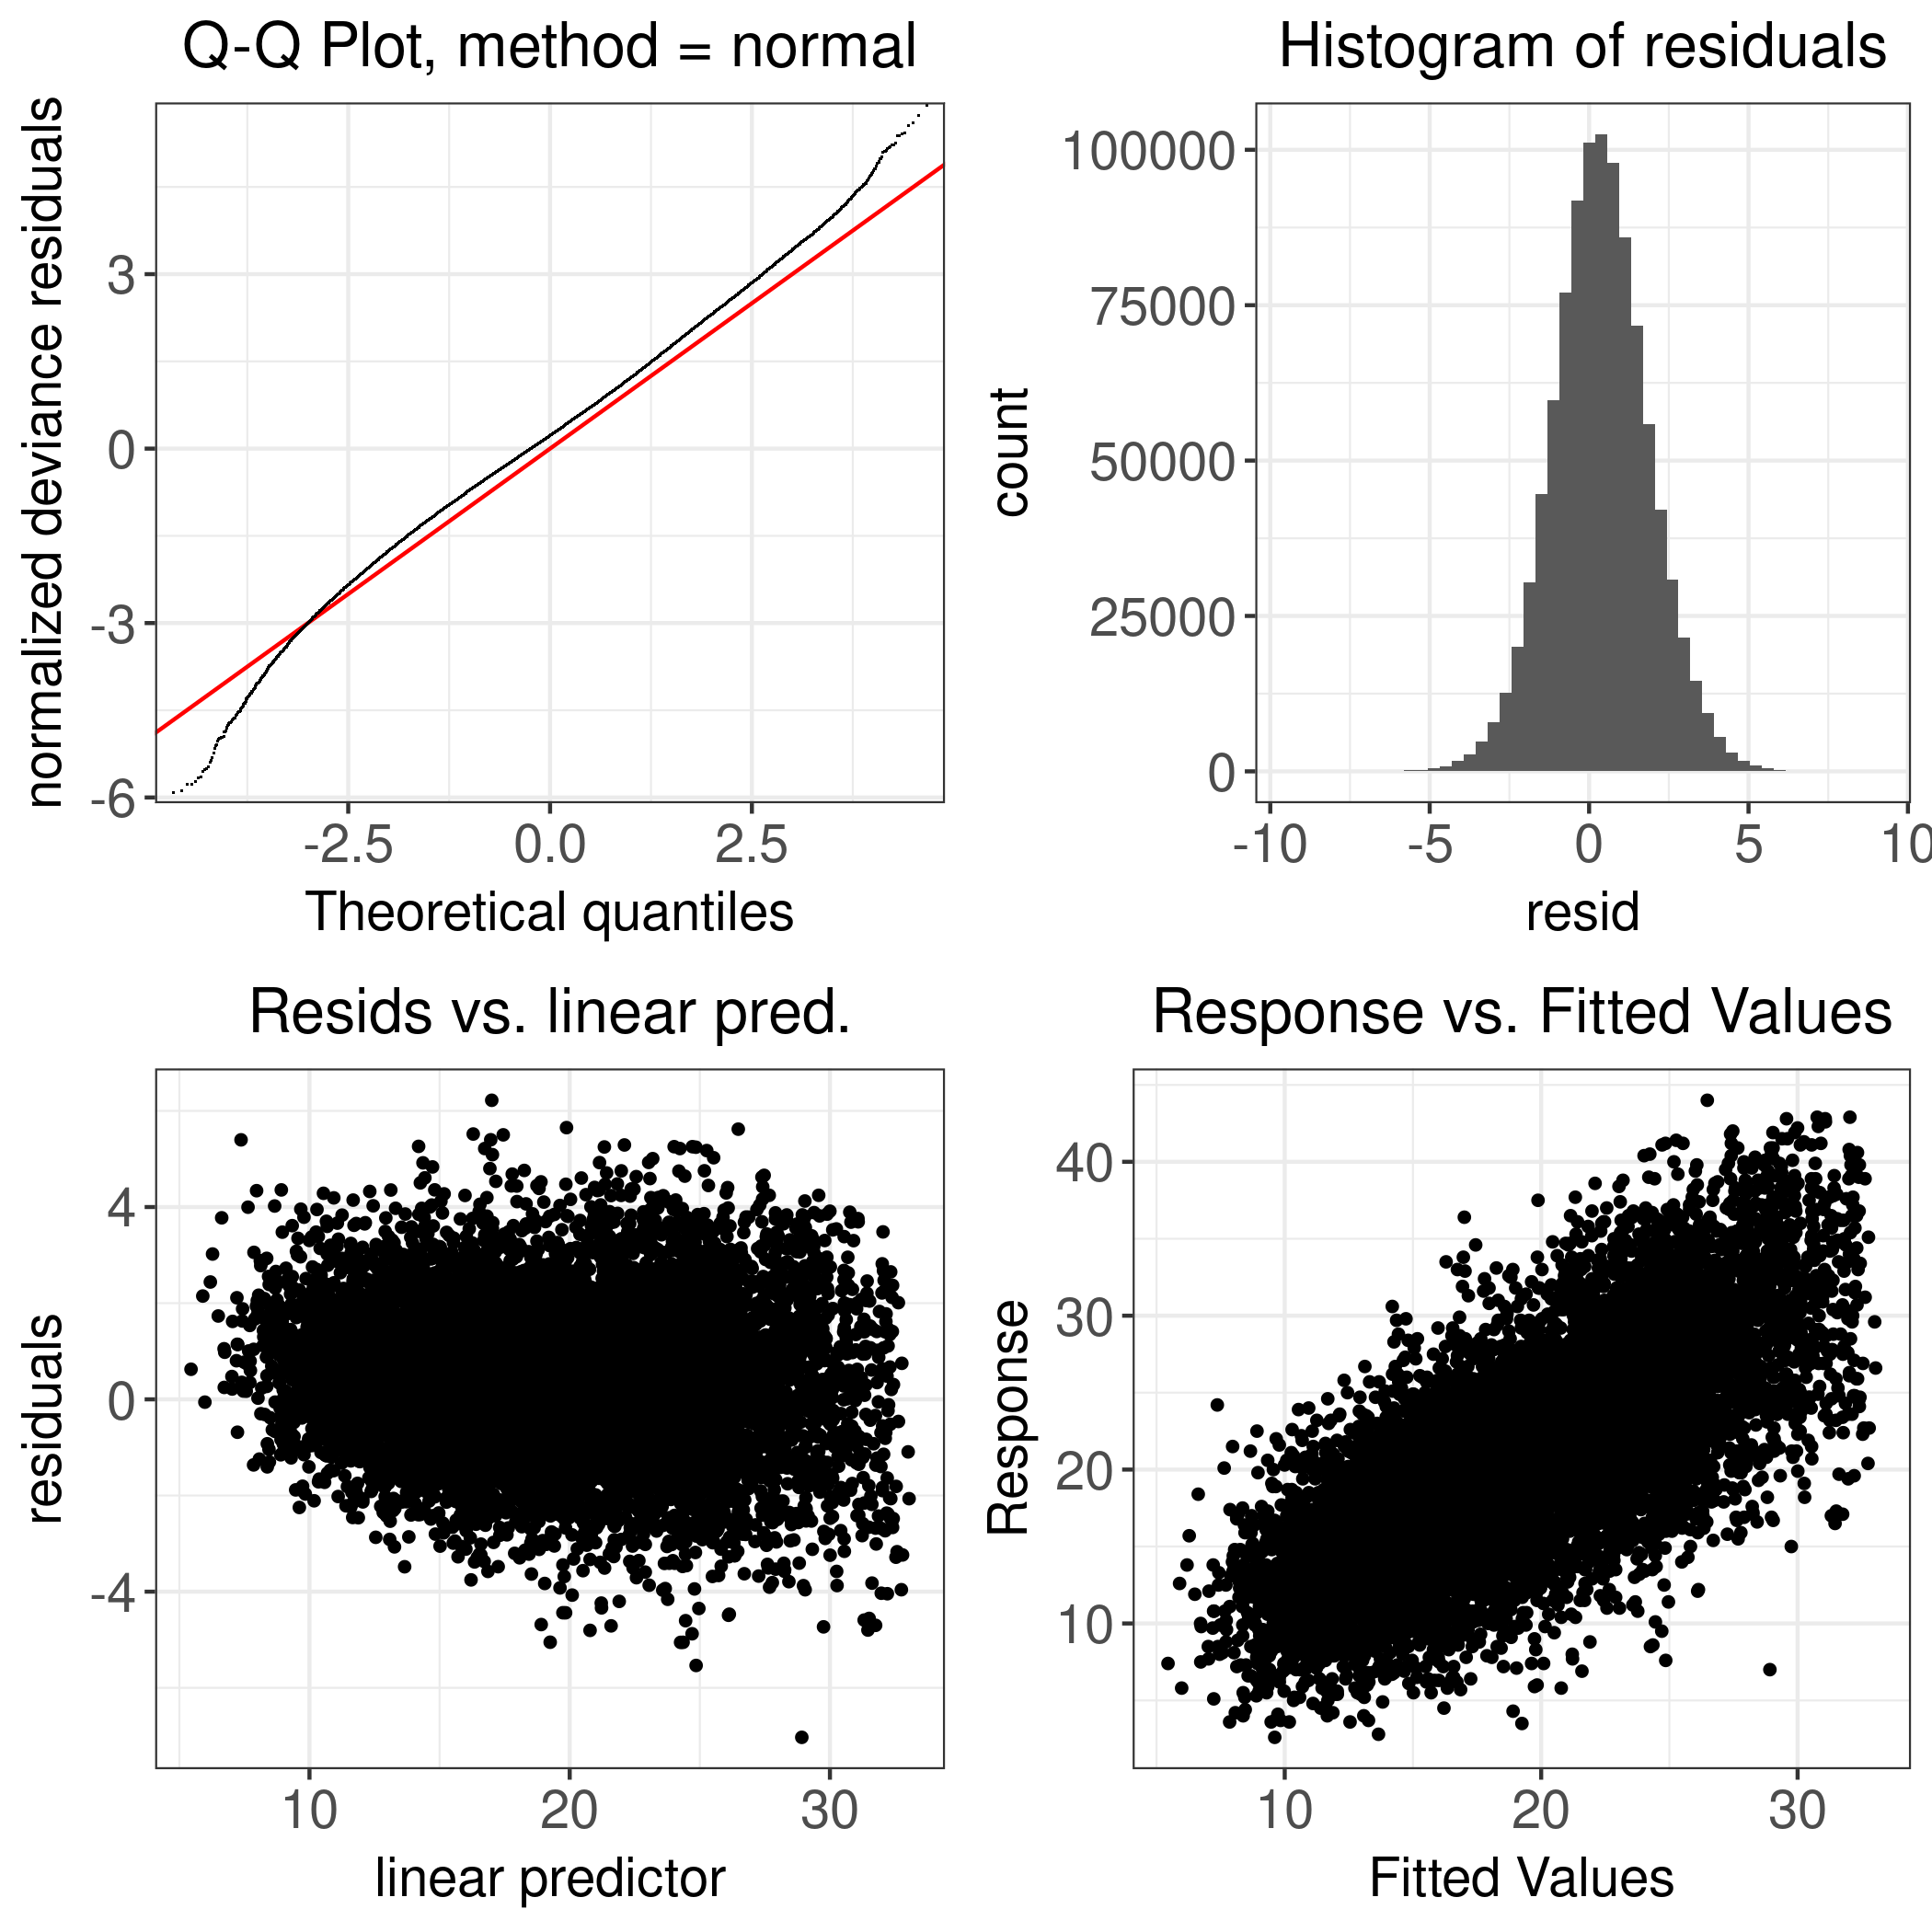
\includegraphics[width=0.6\textwidth]{thesis/figures/models/milk/full/sf_milk_full/sf_milk_full_diagnostics.png}
    \caption[]{Swiss Fleckvieh: Milk Yield - 1984-2023 - Diagnostic Plot}
\end{figure}

\newpage
\paragraph{THI Effect and Lactation Curve} \quad \\
\begin{figure}[H]
    \centering
    \begin{subfigure}[b]{0.45\textwidth}
        \centering
        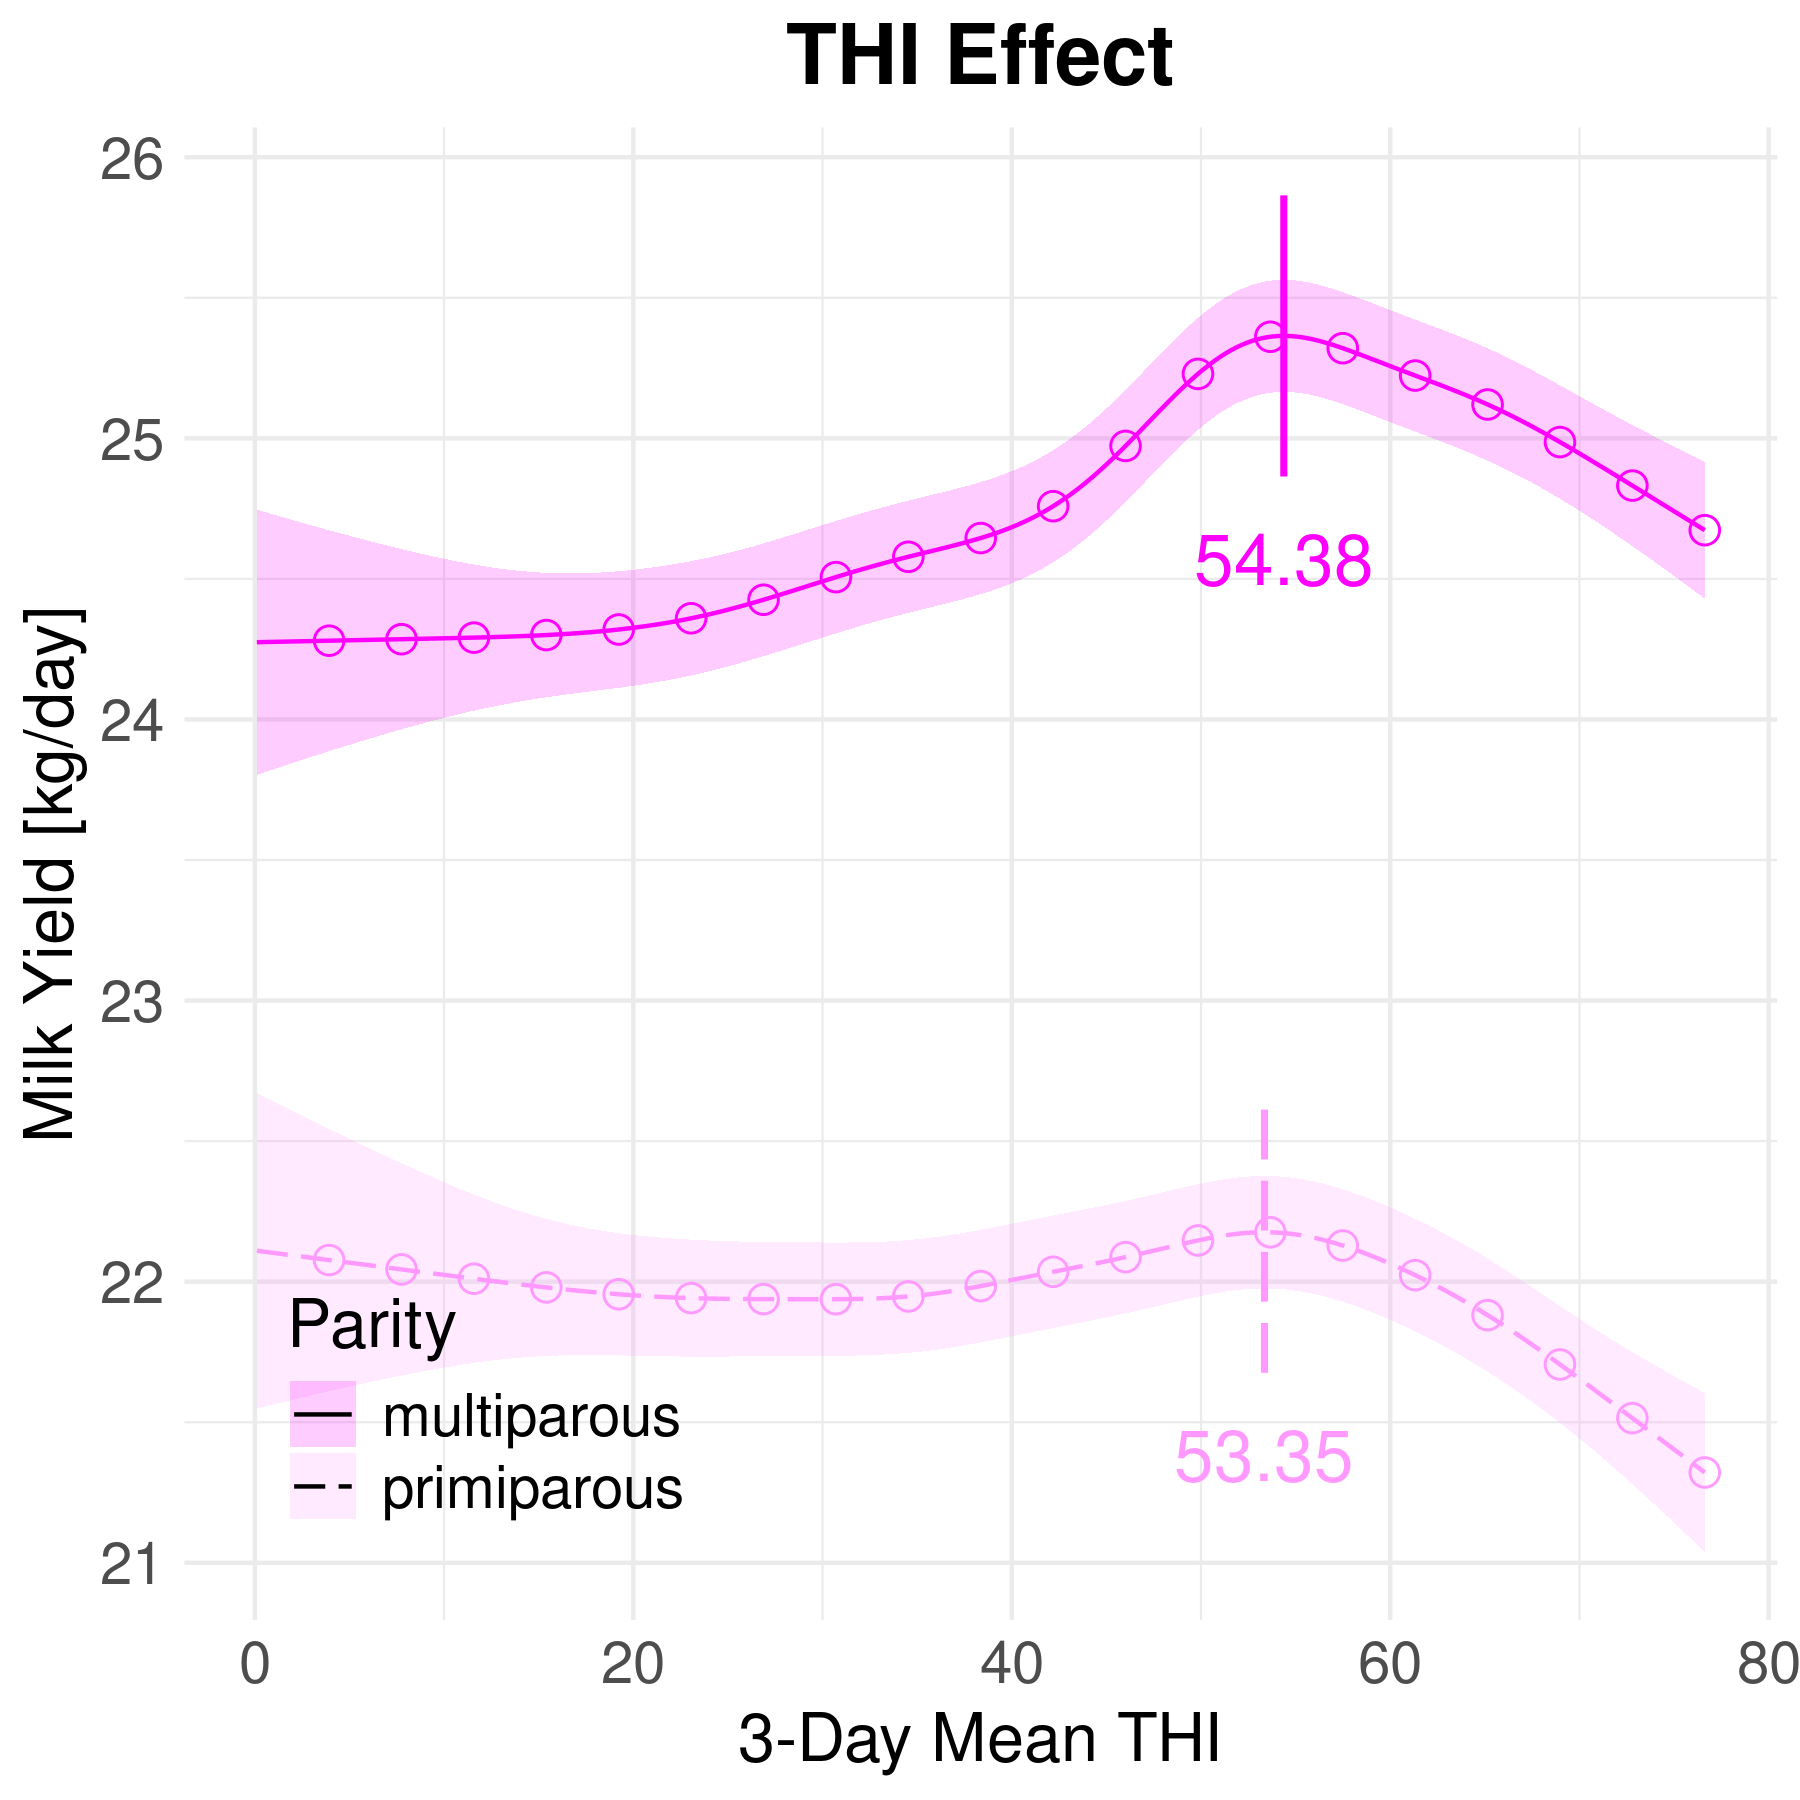
\includegraphics[width=\textwidth]{thesis/figures/models/milk/full/sf_milk_full/sf_milk_full_marginal_thi_milk_combined.png}
    \end{subfigure}
    \hspace{0.05\textwidth} % Optional space between the figures
    \begin{subfigure}[b]{0.45\textwidth}
        \centering
        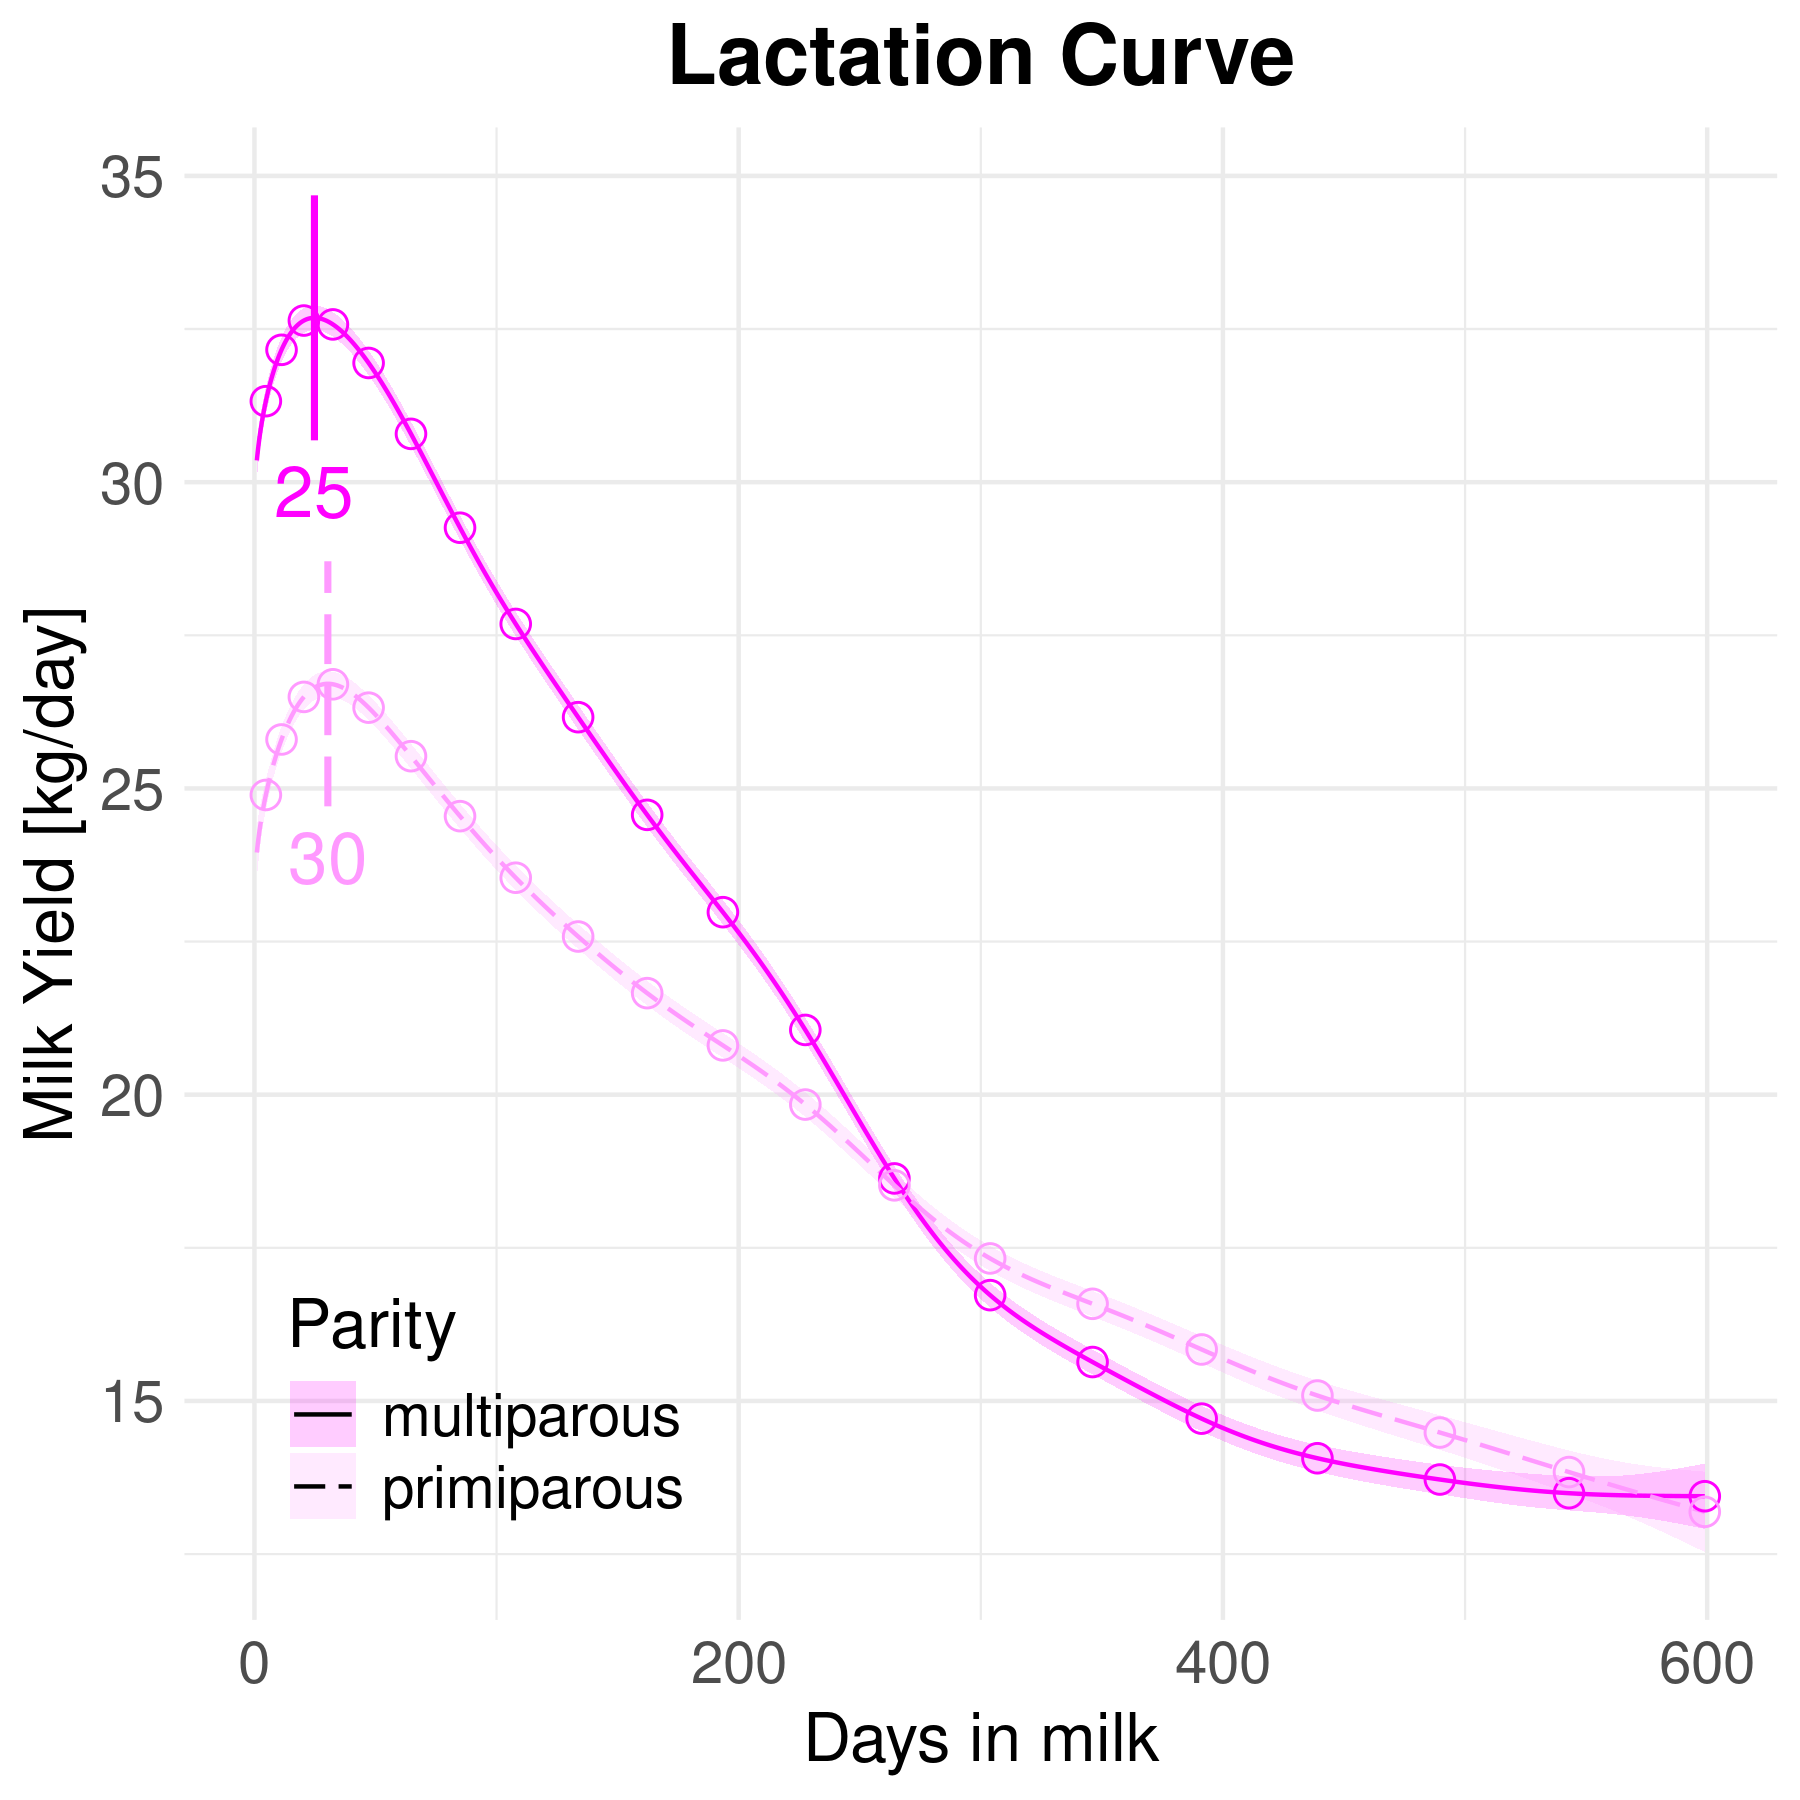
\includegraphics[width=\textwidth]{thesis/figures/models/milk/full/sf_milk_full/sf_milk_full_marginal_dim_milk_combined.png}
    \end{subfigure}
    \begin{subfigure}[b]{0.45\textwidth}
        \centering
        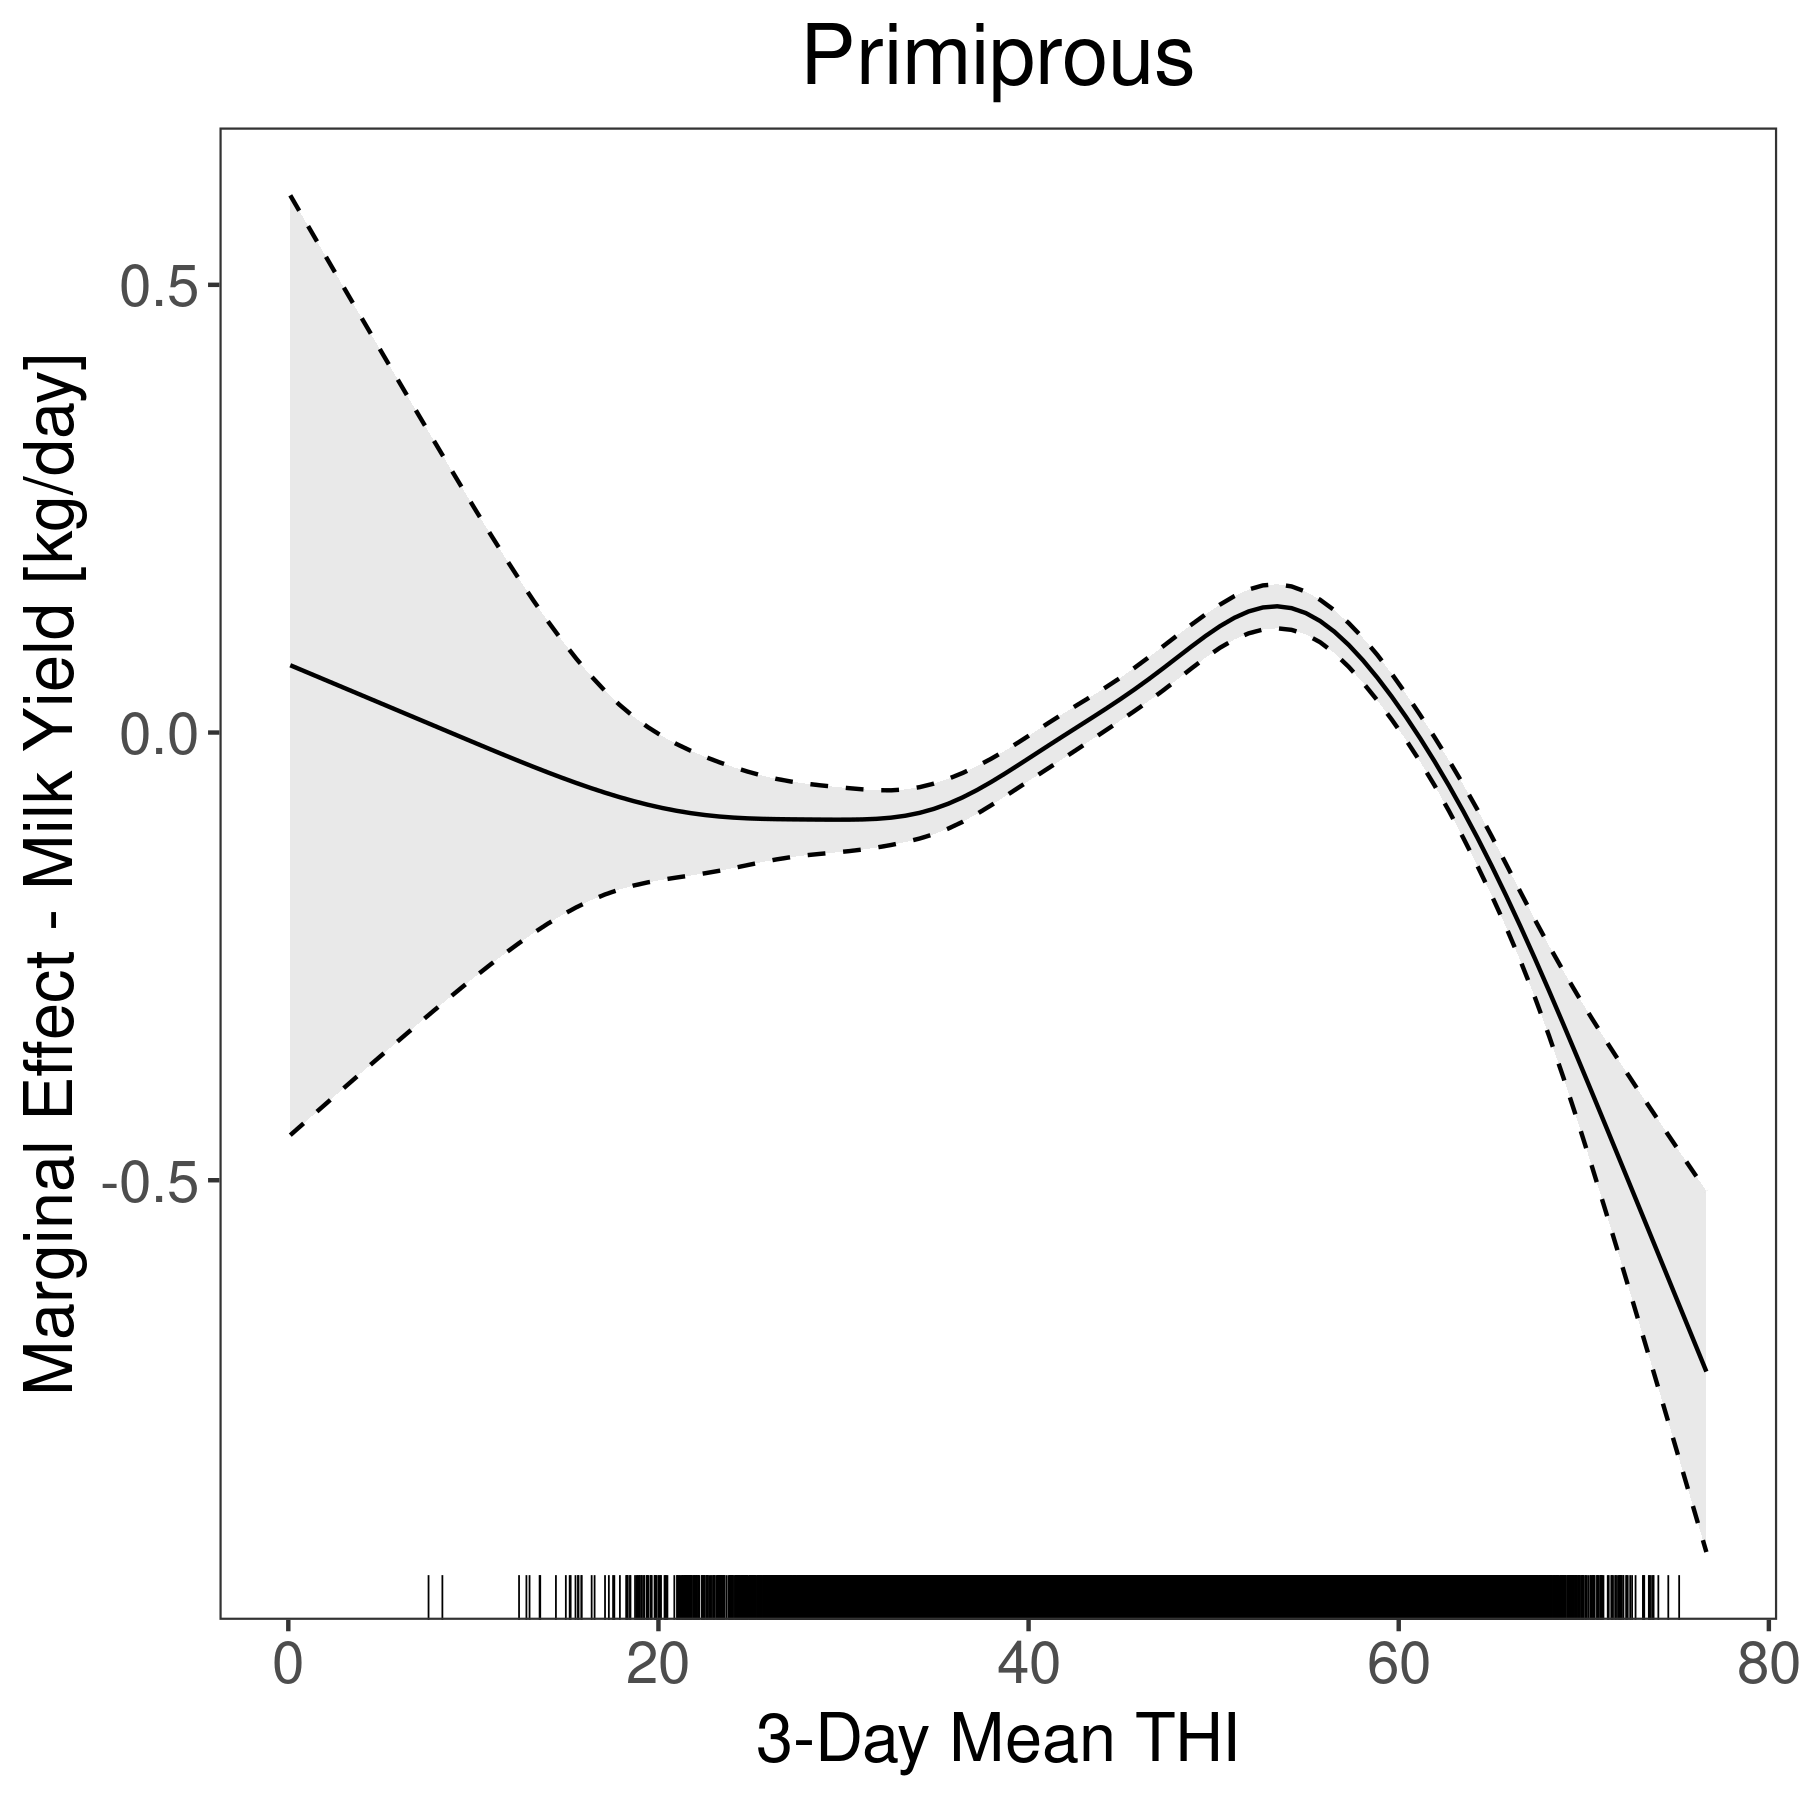
\includegraphics[width=\textwidth]{thesis/figures/models/milk/full/sf_milk_full/sf_milk_full_marginal_thi_milk_primi.png}
    \end{subfigure}
    \hspace{0.05\textwidth} % Optional space between the figures
    \begin{subfigure}[b]{0.45\textwidth}
        \centering
        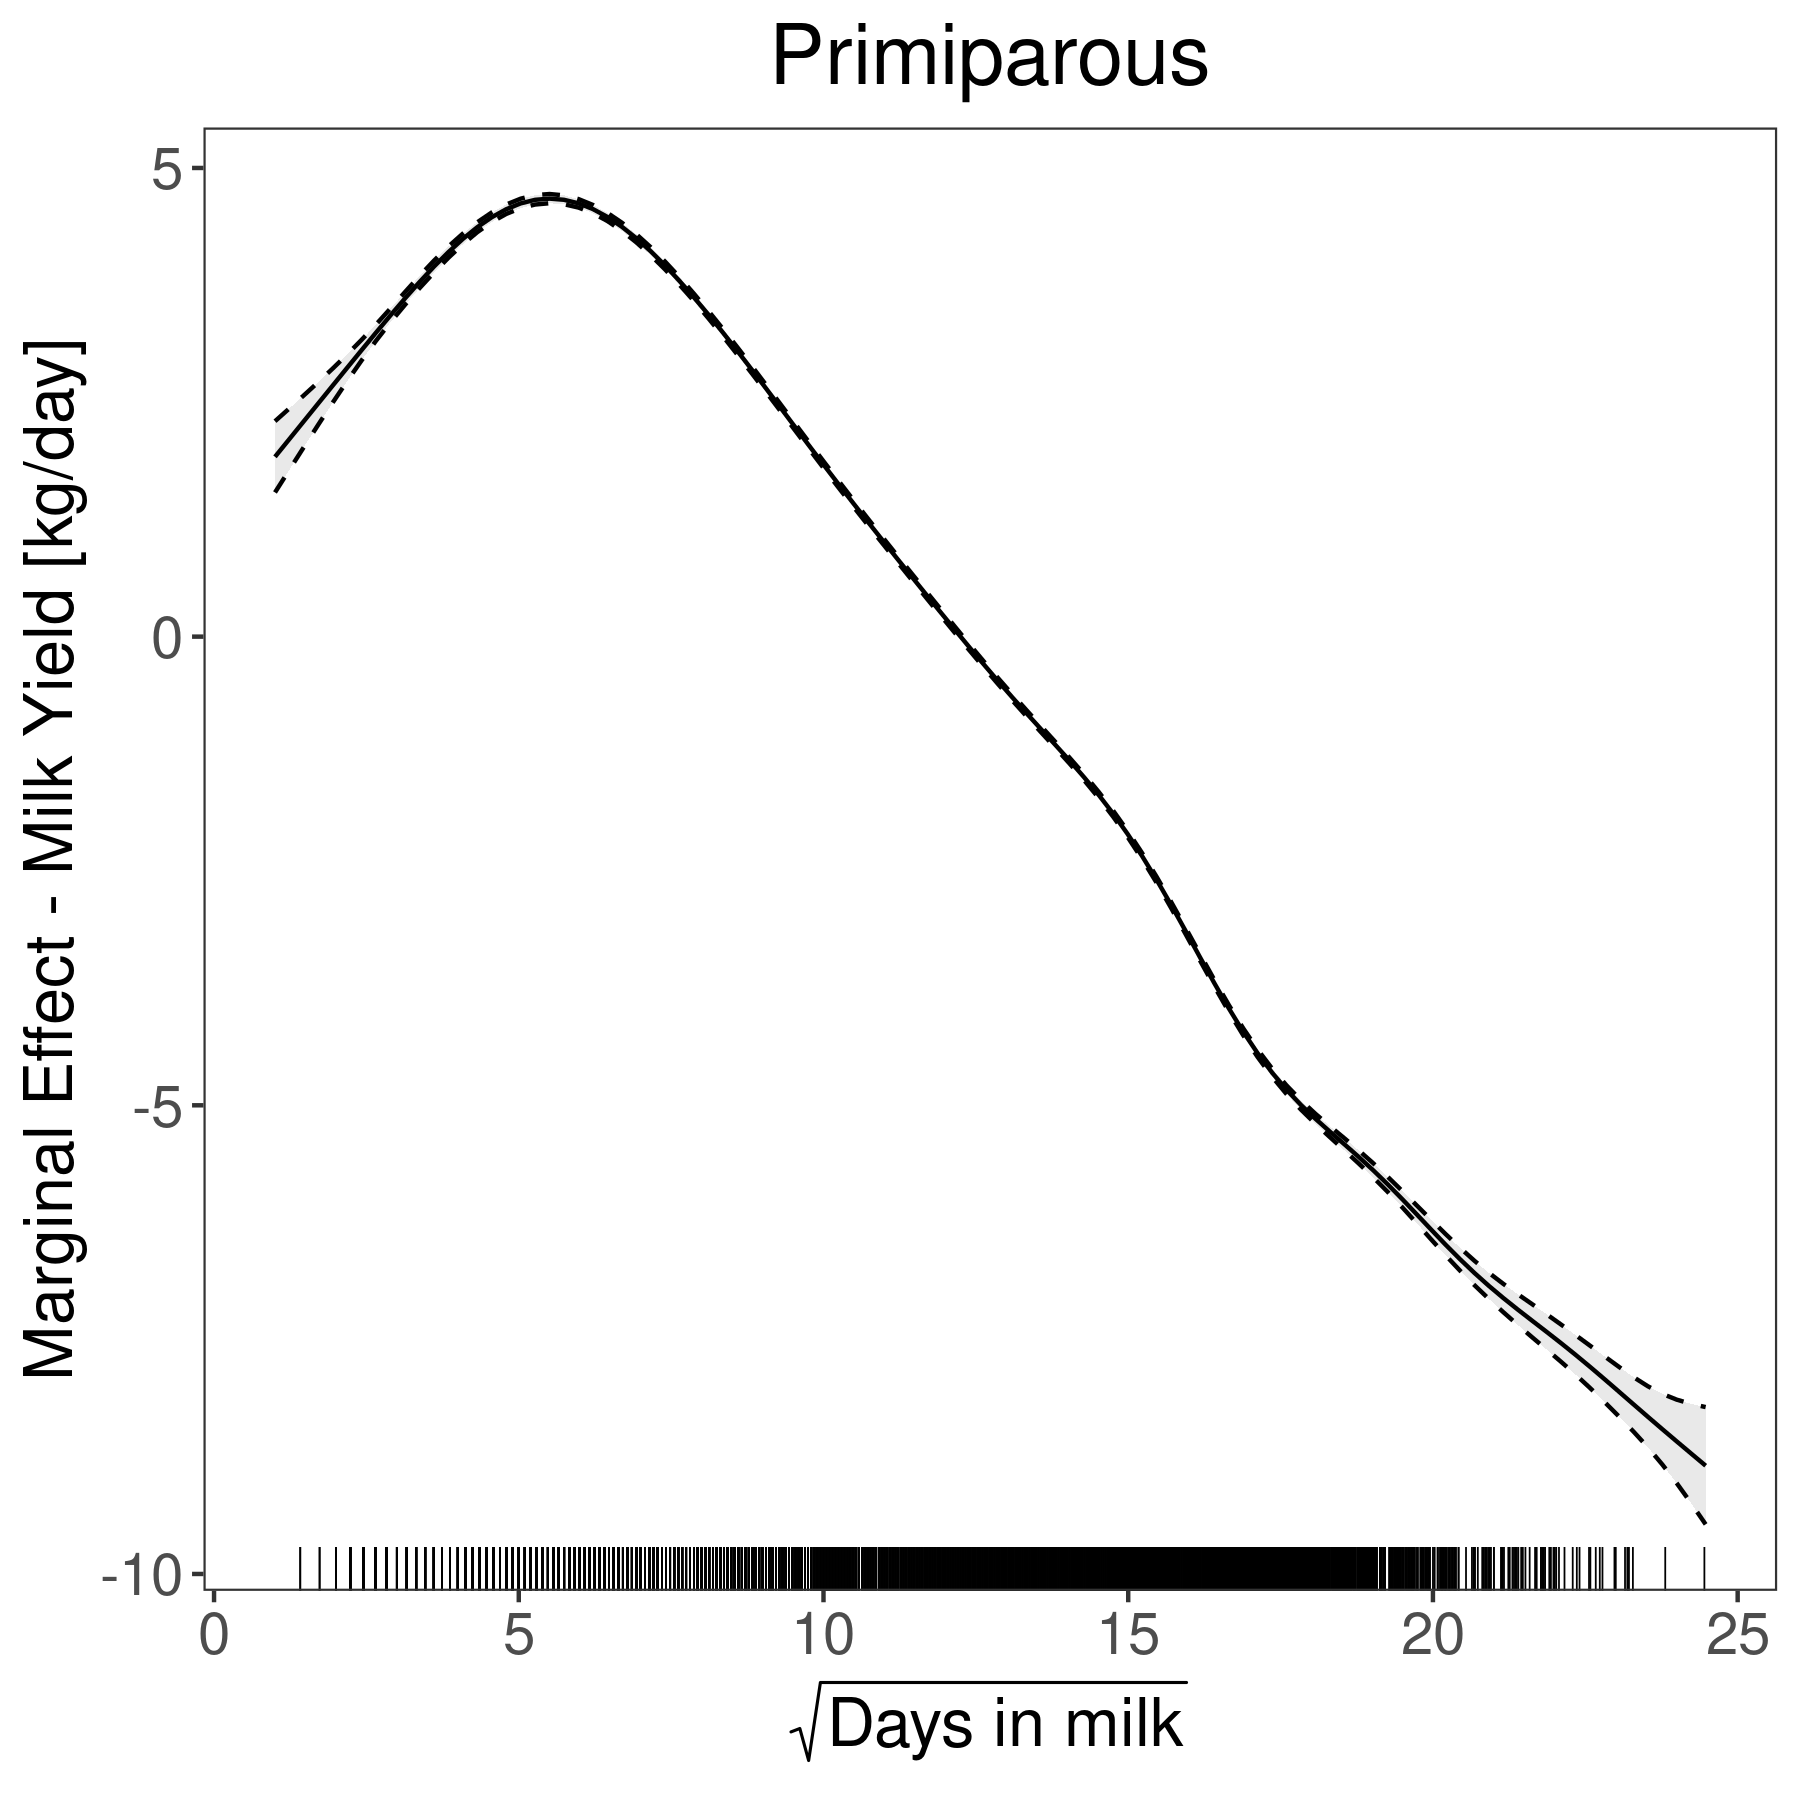
\includegraphics[width=\textwidth]{thesis/figures/models/milk/full/sf_milk_full/sf_milk_full_marginal_dim_milk_primi.png}
    \end{subfigure}
    \begin{subfigure}[b]{0.45\textwidth}
        \centering
        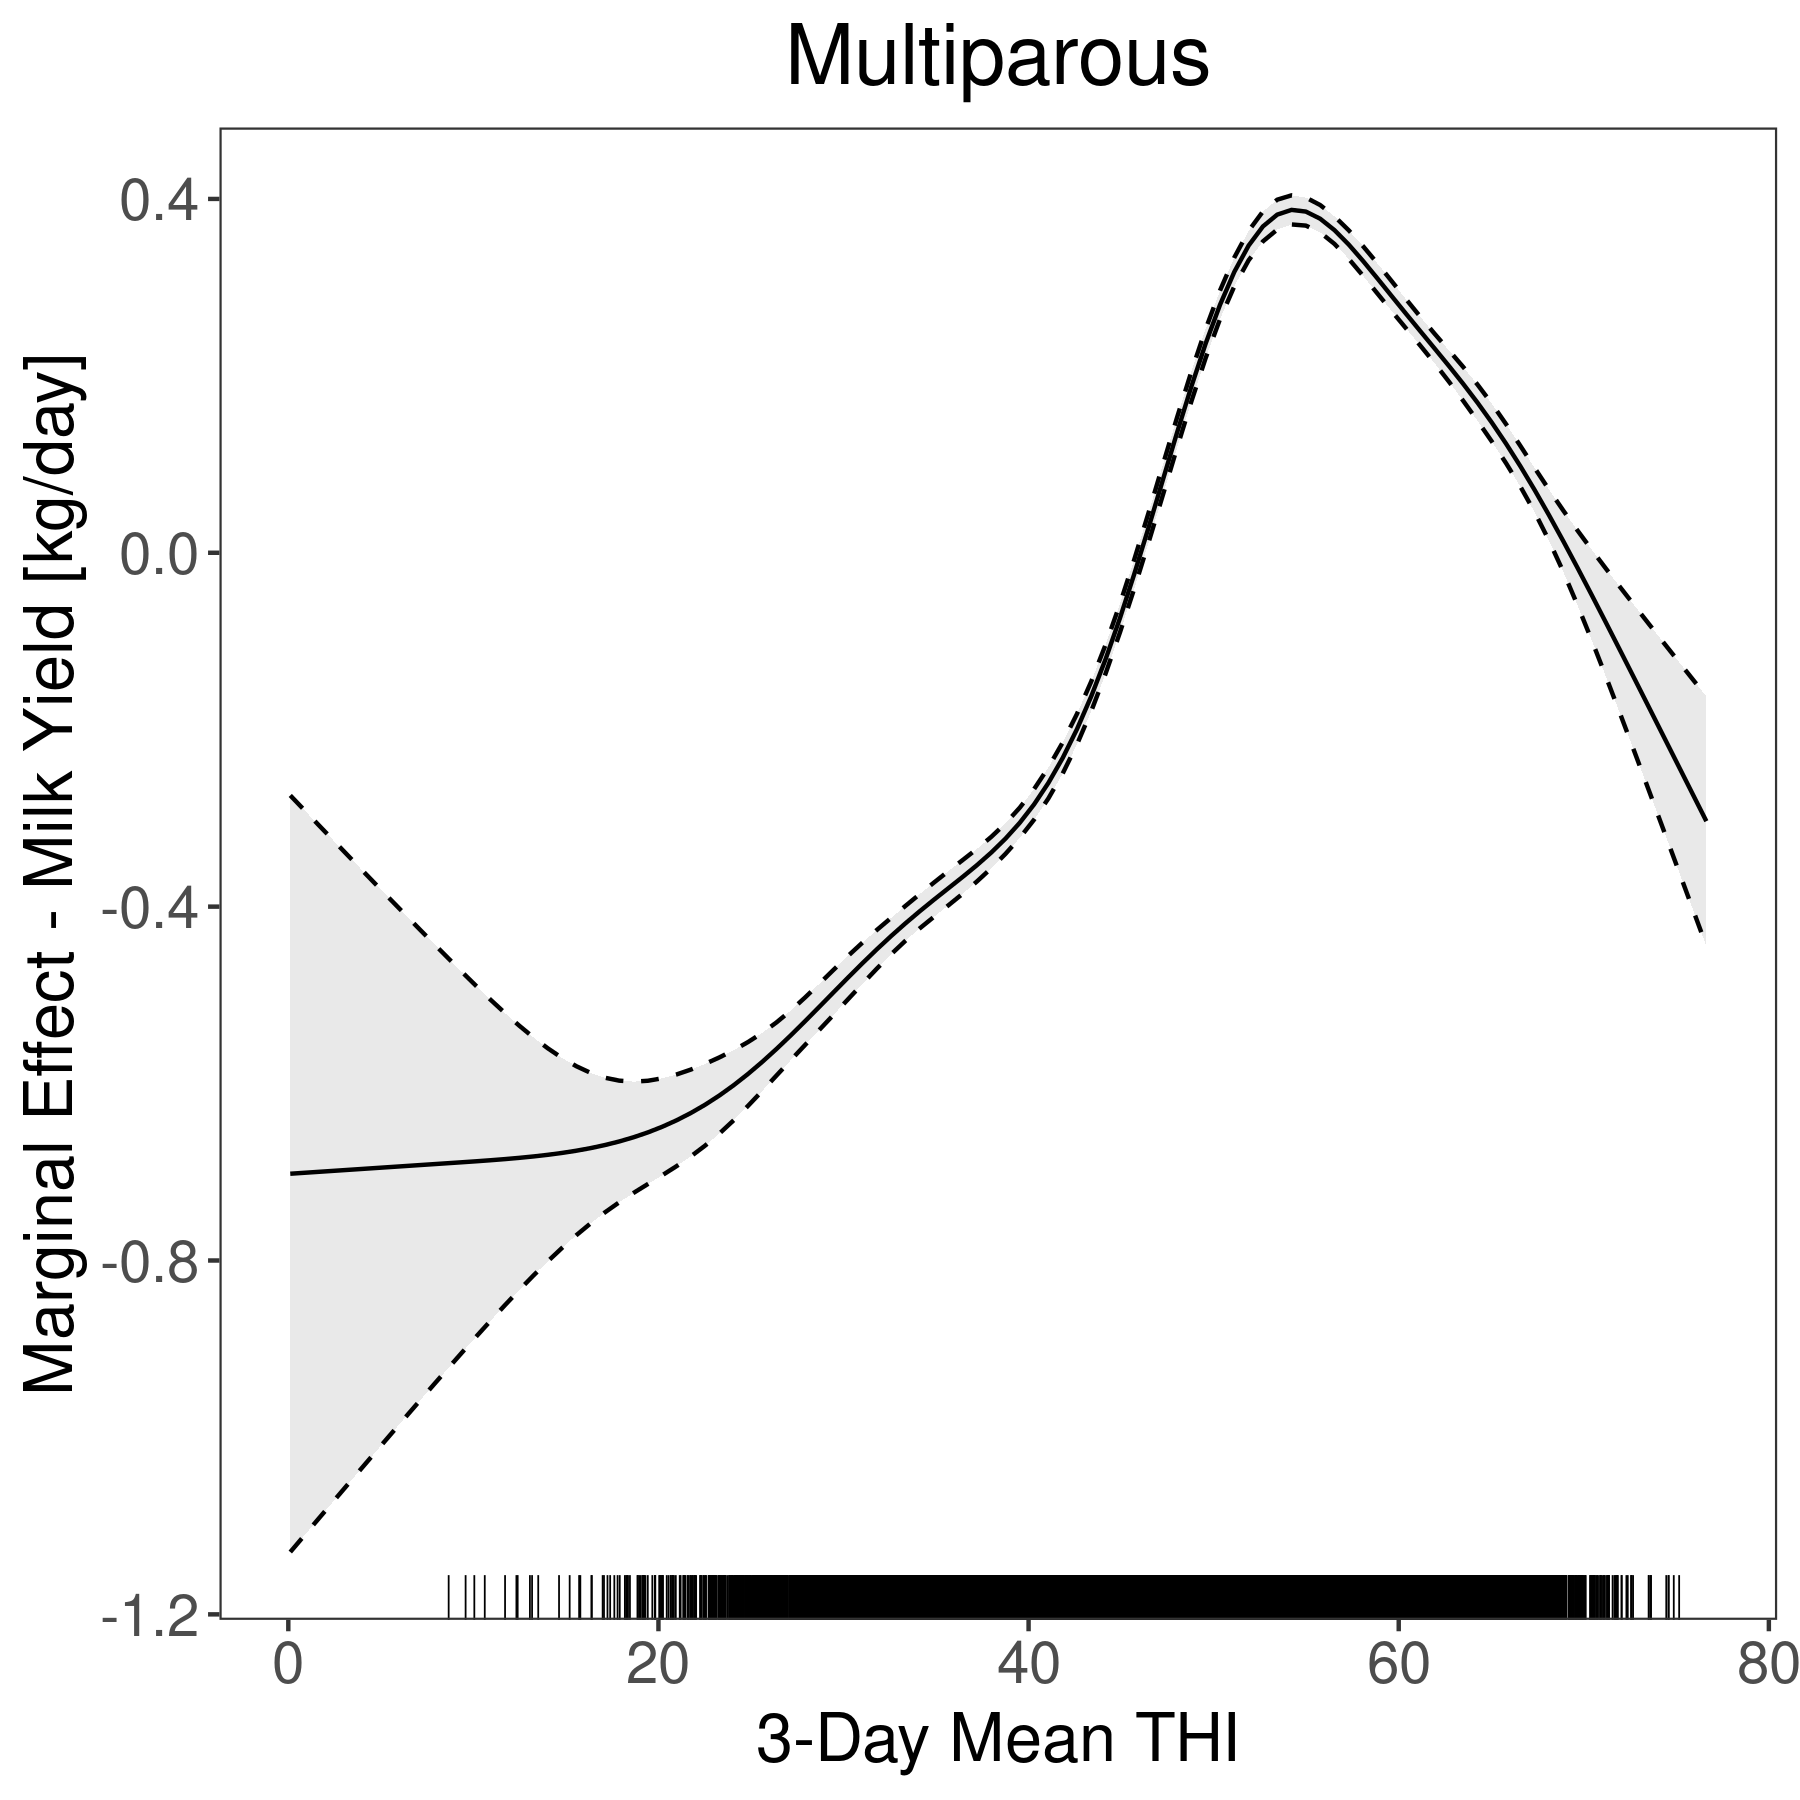
\includegraphics[width=\textwidth]{thesis/figures/models/milk/full/sf_milk_full/sf_milk_full_marginal_thi_milk_multi.png}
    \end{subfigure}
    \hspace{0.05\textwidth} % Optional space between the figures
    \begin{subfigure}[b]{0.45\textwidth}
        \centering
        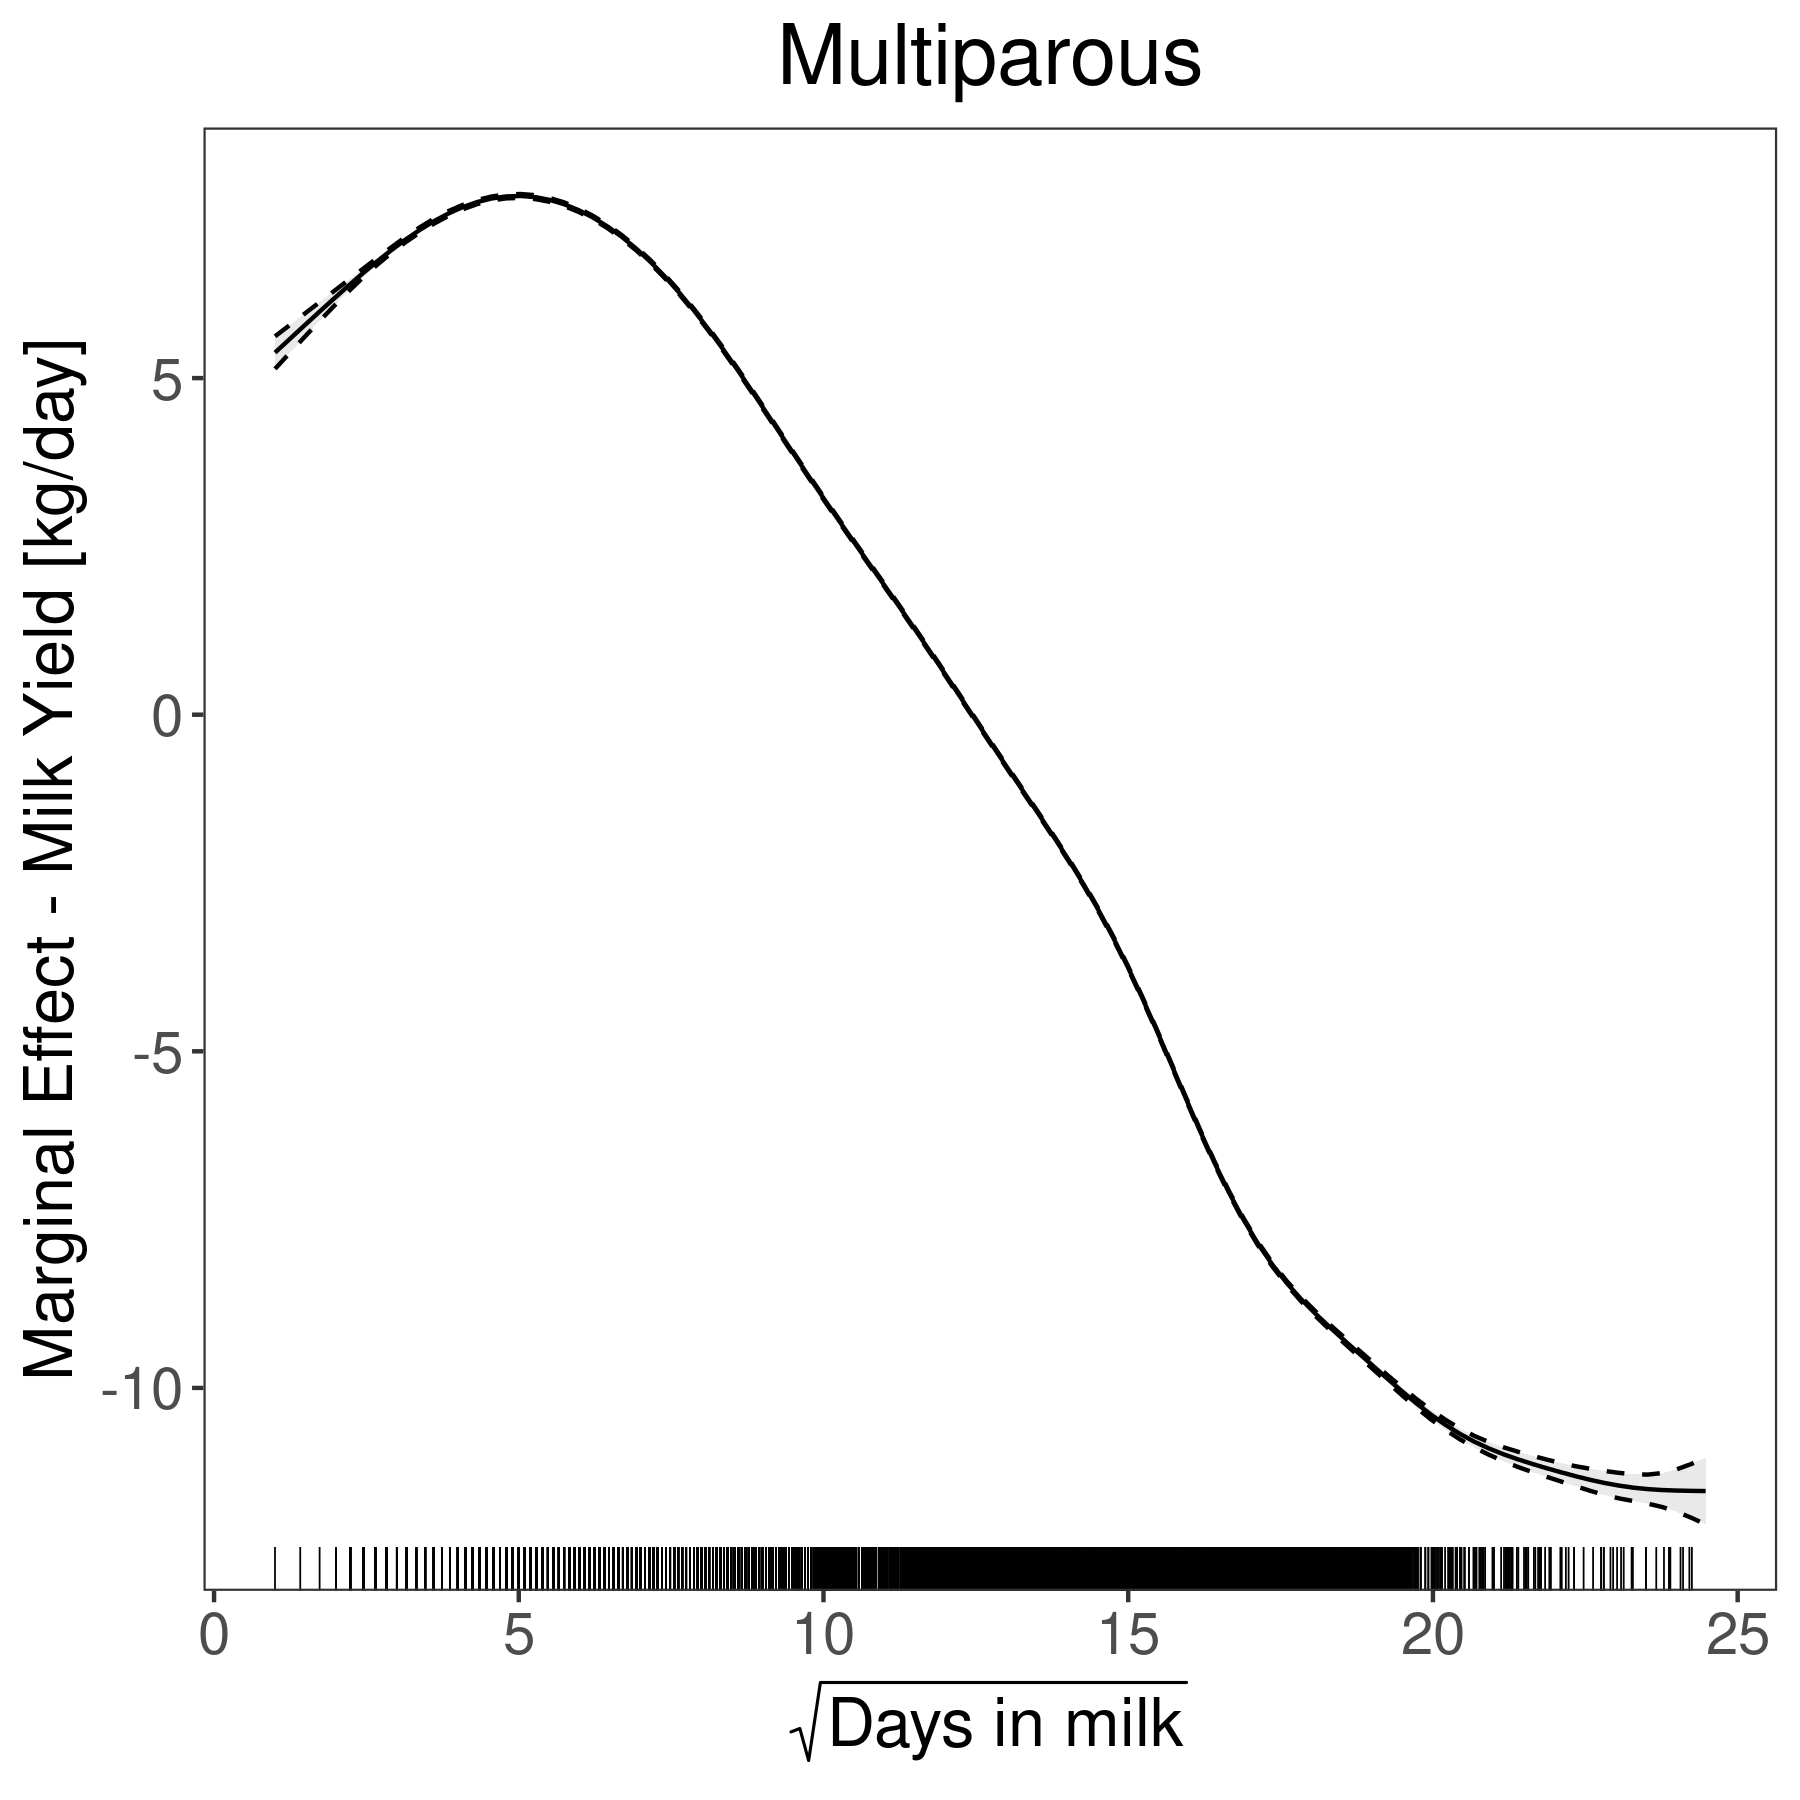
\includegraphics[width=\textwidth]{thesis/figures/models/milk/full/sf_milk_full/sf_milk_full_marginal_dim_milk_multi.png}
    \end{subfigure}
    \caption[]{Swiss Fleckvieh: Milk Yield - 1984 - 2023 - THI Effect and Lactation Curve}
    \label{fig:main}
\end{figure}

\subsection{Split Period: Until 2010 - After 2010}
\addtocontents{toc}{\protect\setcounter{tocdepth}{-1}}
\subsubsection{Split Period: 1984 - 2010}\label{model:sf_milk_before}
\paragraph{Model Summary} \quad \\

    \begin{table}[H]
    \centering
    \begin{tabular}{lrrrr}
    \textbf{A. parametric coefficients} & Estimate & Std. Error & t-value & p-value \\ 
       \hline
       \hline
      (Intercept) & 16.9035 & 0.3658 & 46.2066 & $<$ 0.0001 \\ 
      parityprimiparous & -2.7346 & 0.0138 & -198.6779 & $<$ 0.0001 \\ 
      year1985 & 0.4515 & 0.2804 & 1.6103 & 0.1073 \\ 
      year1986 & 0.3178 & 0.3341 & 0.9510 & 0.3416 \\ 
      year1987 & 0.2380 & 0.3534 & 0.6736 & 0.5006 \\ 
      year1988 & 0.0232 & 0.3872 & 0.0600 & 0.9522 \\ 
      year1989 & 0.7996 & 0.3910 & 2.0451 & 0.0408 \\ 
      year1990 & 1.1652 & 0.3833 & 3.0397 & 0.0024 \\ 
      year1991 & 1.4053 & 0.3711 & 3.7868 & 0.0002 \\ 
      year1992 & 1.6217 & 0.3462 & 4.6846 & $<$ 0.0001 \\ 
      year1993 & 1.6209 & 0.3497 & 4.6347 & $<$ 0.0001 \\ 
      year1994 & 1.6641 & 0.3651 & 4.5578 & $<$ 0.0001 \\ 
      year1995 & 1.9199 & 0.4094 & 4.6900 & $<$ 0.0001 \\ 
      year1996 & 2.1351 & 0.4138 & 5.1595 & $<$ 0.0001 \\ 
      year1997 & 2.5677 & 0.4256 & 6.0334 & $<$ 0.0001 \\ 
      year1998 & 3.4175 & 0.4545 & 7.5191 & $<$ 0.0001 \\ 
      year1999 & 3.5626 & 0.4510 & 7.9000 & $<$ 0.0001 \\ 
      year2000 & 3.7240 & 0.4591 & 8.1121 & $<$ 0.0001 \\ 
      year2001 & 4.0732 & 0.4673 & 8.7165 & $<$ 0.0001 \\ 
      year2002 & 4.3548 & 0.4508 & 9.6605 & $<$ 0.0001 \\ 
      year2003 & 4.8981 & 0.4394 & 11.1471 & $<$ 0.0001 \\ 
      year2004 & 5.4440 & 0.4520 & 12.0437 & $<$ 0.0001 \\ 
      year2005 & 5.7965 & 0.4626 & 12.5311 & $<$ 0.0001 \\ 
      year2006 & 5.8531 & 0.4836 & 12.1040 & $<$ 0.0001 \\ 
      year2007 & 5.6656 & 0.4880 & 11.6103 & $<$ 0.0001 \\ 
      year2008 & 5.9522 & 0.4987 & 11.9352 & $<$ 0.0001 \\ 
      year2009 & 6.4429 & 0.5211 & 12.3638 & $<$ 0.0001 \\ 
      year2010 & 7.0430 & 0.5707 & 12.3418 & $<$ 0.0001 \\ 
       \hline
    \textbf{B. smooth terms} & edf & Ref.df & F-value & p-value \\ 
    \hline
    \hline
      s(thi\_mean\_t0\_3d):paritymultiparous & 8.8565 & 8.8565 & 828.8023 & $<$ 0.0001 \\ 
      s(thi\_mean\_t0\_3d):parityprimiparous & 6.8104 & 6.8104 & 36.0865 & $<$ 0.0001 \\ 
      s(days\_in\_milk\_t):paritymultiparous & 14.2457 & 14.2457 & 139197.9545 & $<$ 0.0001 \\ 
      s(days\_in\_milk\_t):parityprimiparous & 13.2024 & 13.2024 & 14397.4338 & $<$ 0.0001 \\  
       \hline
    \end{tabular}
    \caption[]{Swiss Fleckvieh: Milk Yield - 1984-2010 - GAMM model summary without random effect terms.}
    \end{table}

\newpage
\begin{table}[H]
\centering
\begin{tabular}
{l | r | r | r | r}
\textbf{Smooth Term Fixed Effect} & Est. & SE & z & p\\
\hline
\hline
s(thi\_mean\_t0\_3d):multiFx1 & 0.2333 & 0.0852 & 2.74 & 0.0062\\
s(thi\_mean\_t0\_3d):primiFx1 & 0.2388 & 0.0987 & 2.42 & 0.0155\\
s(days\_in\_milk\_):multiFx1 & 1.3398 & 0.5299 & 2.53 & 0.0114\\
s(days\_in\_milk\_):primiFx1 & 0.3073 & 0.5533 & 0.56 & 0.5786\\
\hline
\textbf{Variance Component} & Estimated $\sigma$ & & & \\
\hline
\hline
$\sigma_\alpha$ & 2.5865 & & & \\
$\sigma_\iota$ & 0.8711 & & & \\
$\sigma_\phi$ & 2.5999 & & & \\
s(thi\_mean\_t0\_3d):multi &  3.8918 & & & \\
s(days\_in\_milk\_):primi & 5.4281 & & & \\
s(days\_in\_milk\_):multi & 7.5874 & & & \\
s(thi\_mean\_t0\_3d):primi & 1.1463 & & & \\
Residual & 2.9720 & & & \\
\end{tabular}
\caption[]{Swiss Fleckvieh: Milk Yield - 1984-2010 - Mixed Model Summary - Smooth Terms and Random Effects.}
\end{table}


\paragraph{Model Diagnostics} \quad \\
\begin{figure}[H]
    \centering
    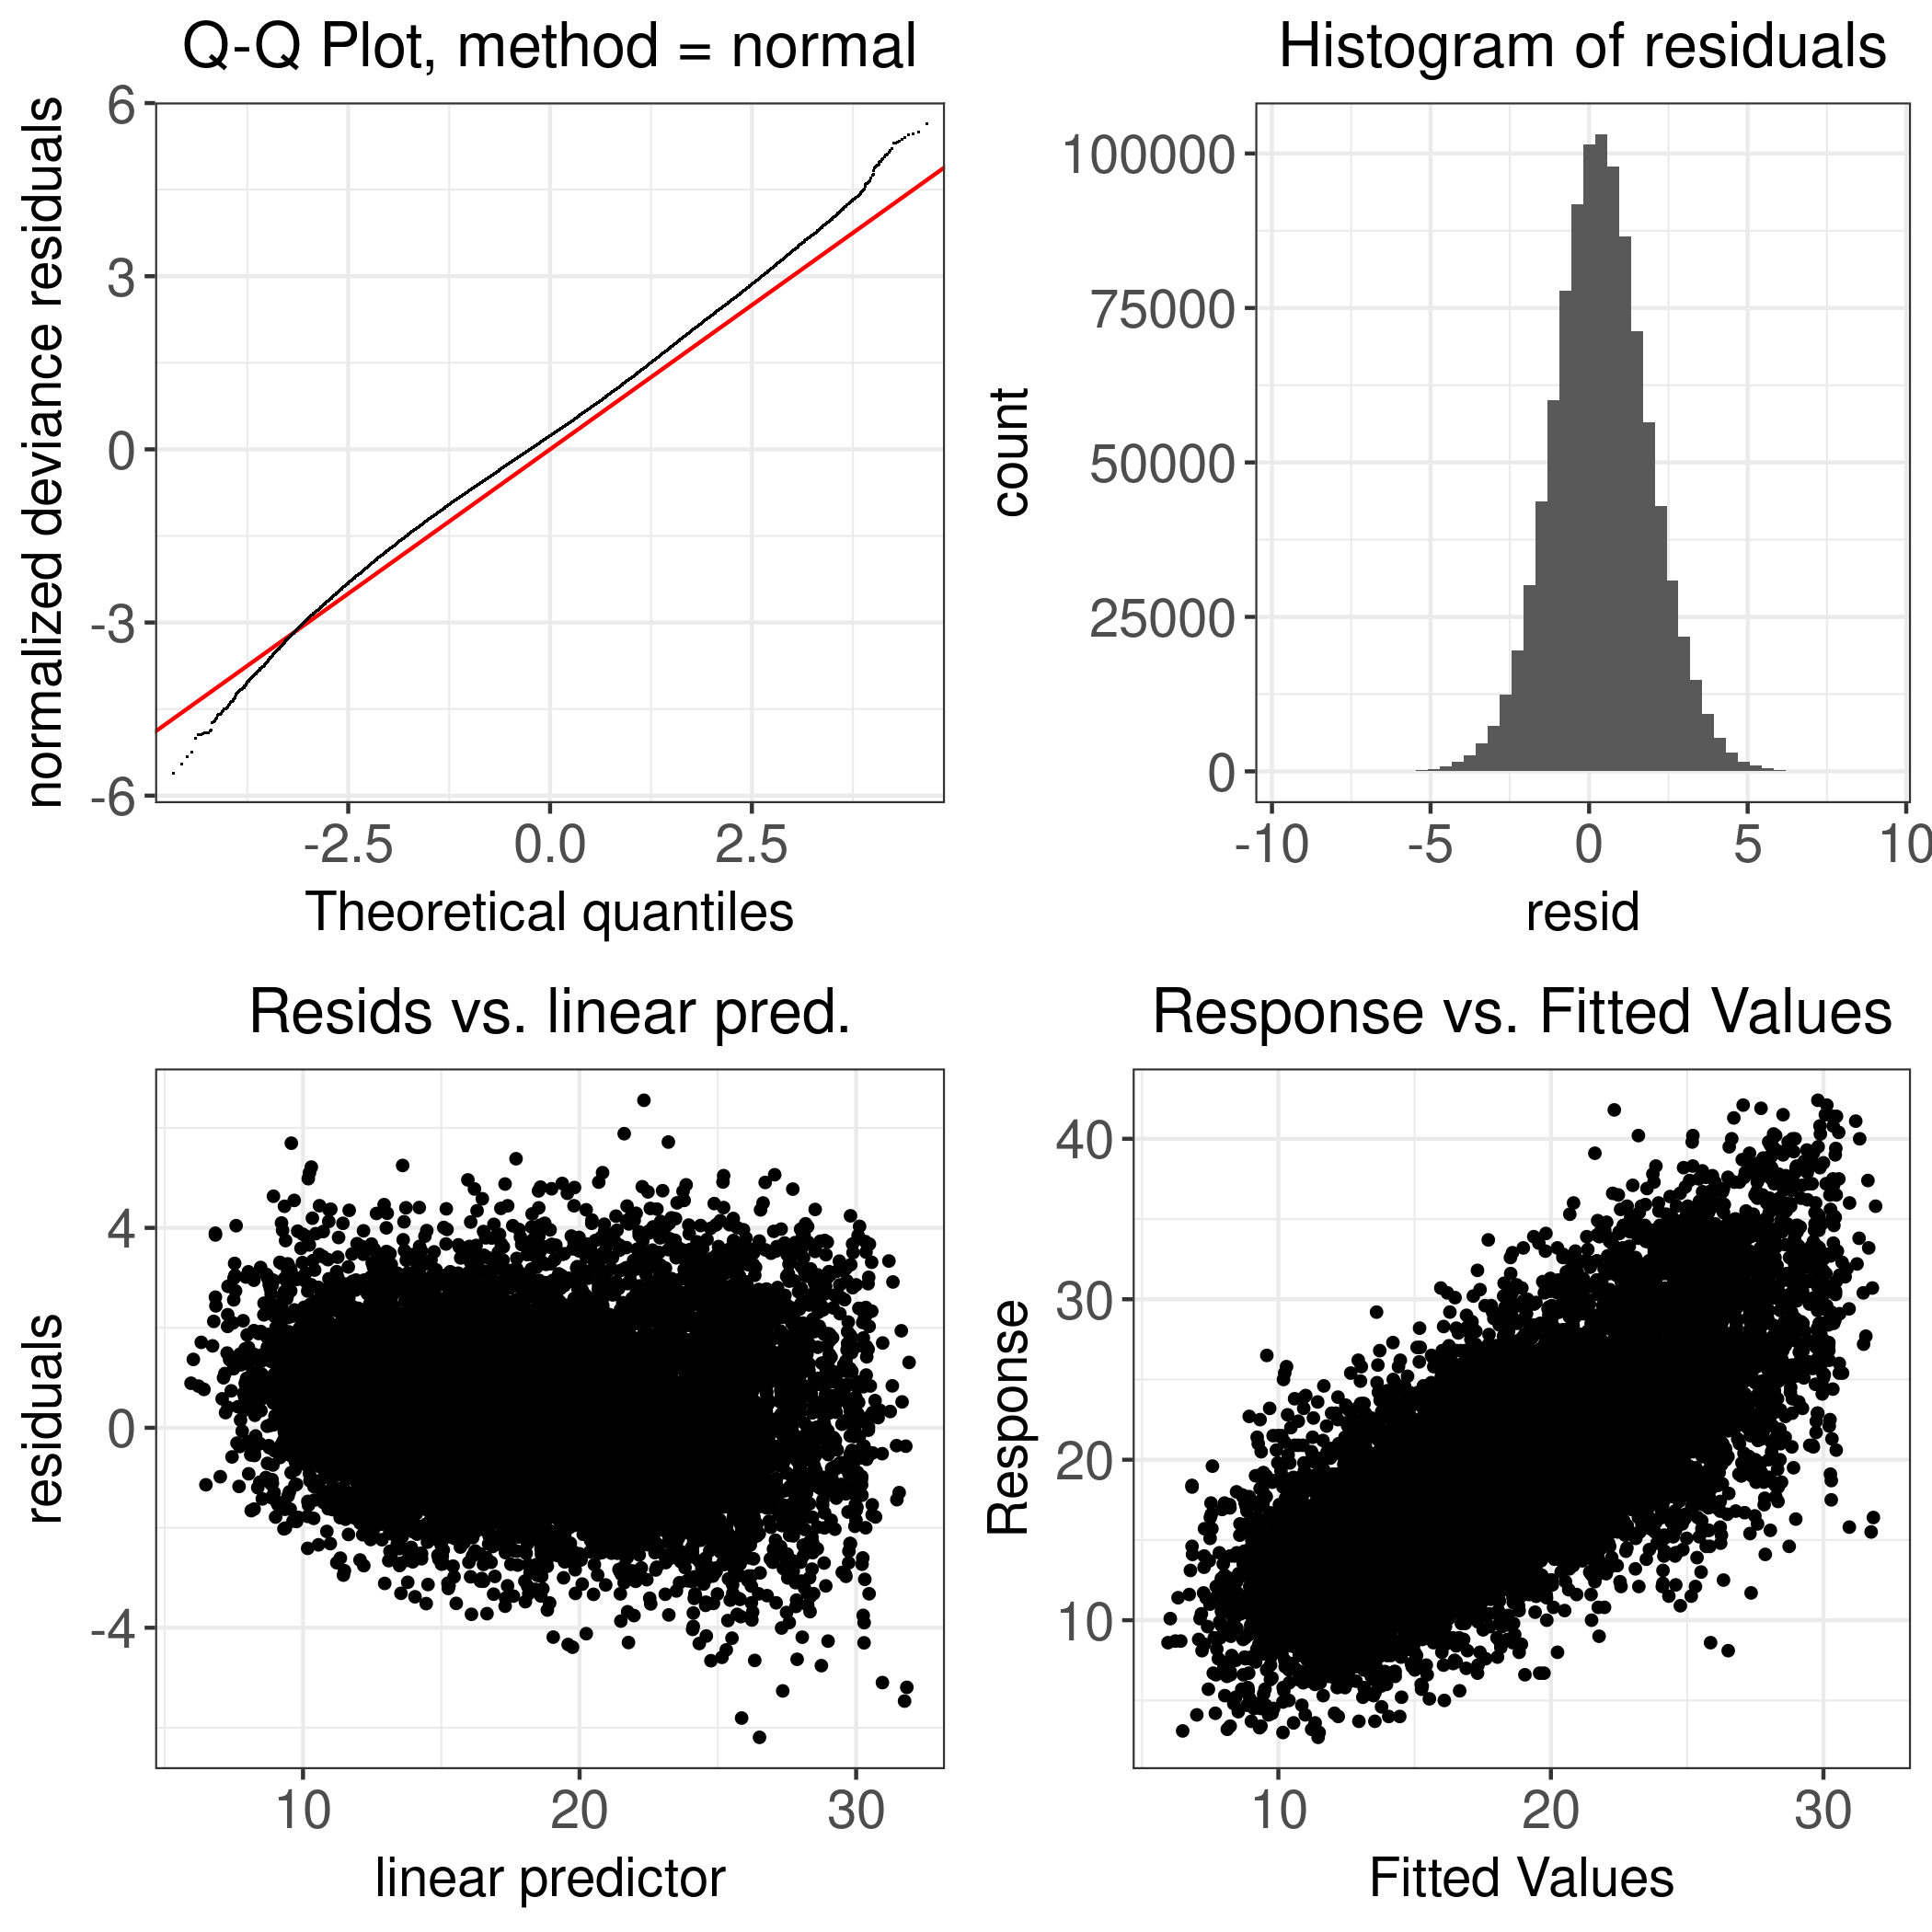
\includegraphics[width=0.6\textwidth]{thesis/figures/models/milk/before2010/sf_milk_before2010/sf_milk_before2010_diagnostics.png}
    \caption[]{Swiss Fleckvieh: Milk Yield - 1984-2010 - Diagnostic Plot}
\end{figure}

\newpage
\paragraph{THI Effect and Lactation Curve} \quad \\
\begin{figure}[H]
    \centering
    \begin{subfigure}[b]{0.45\textwidth}
        \centering
        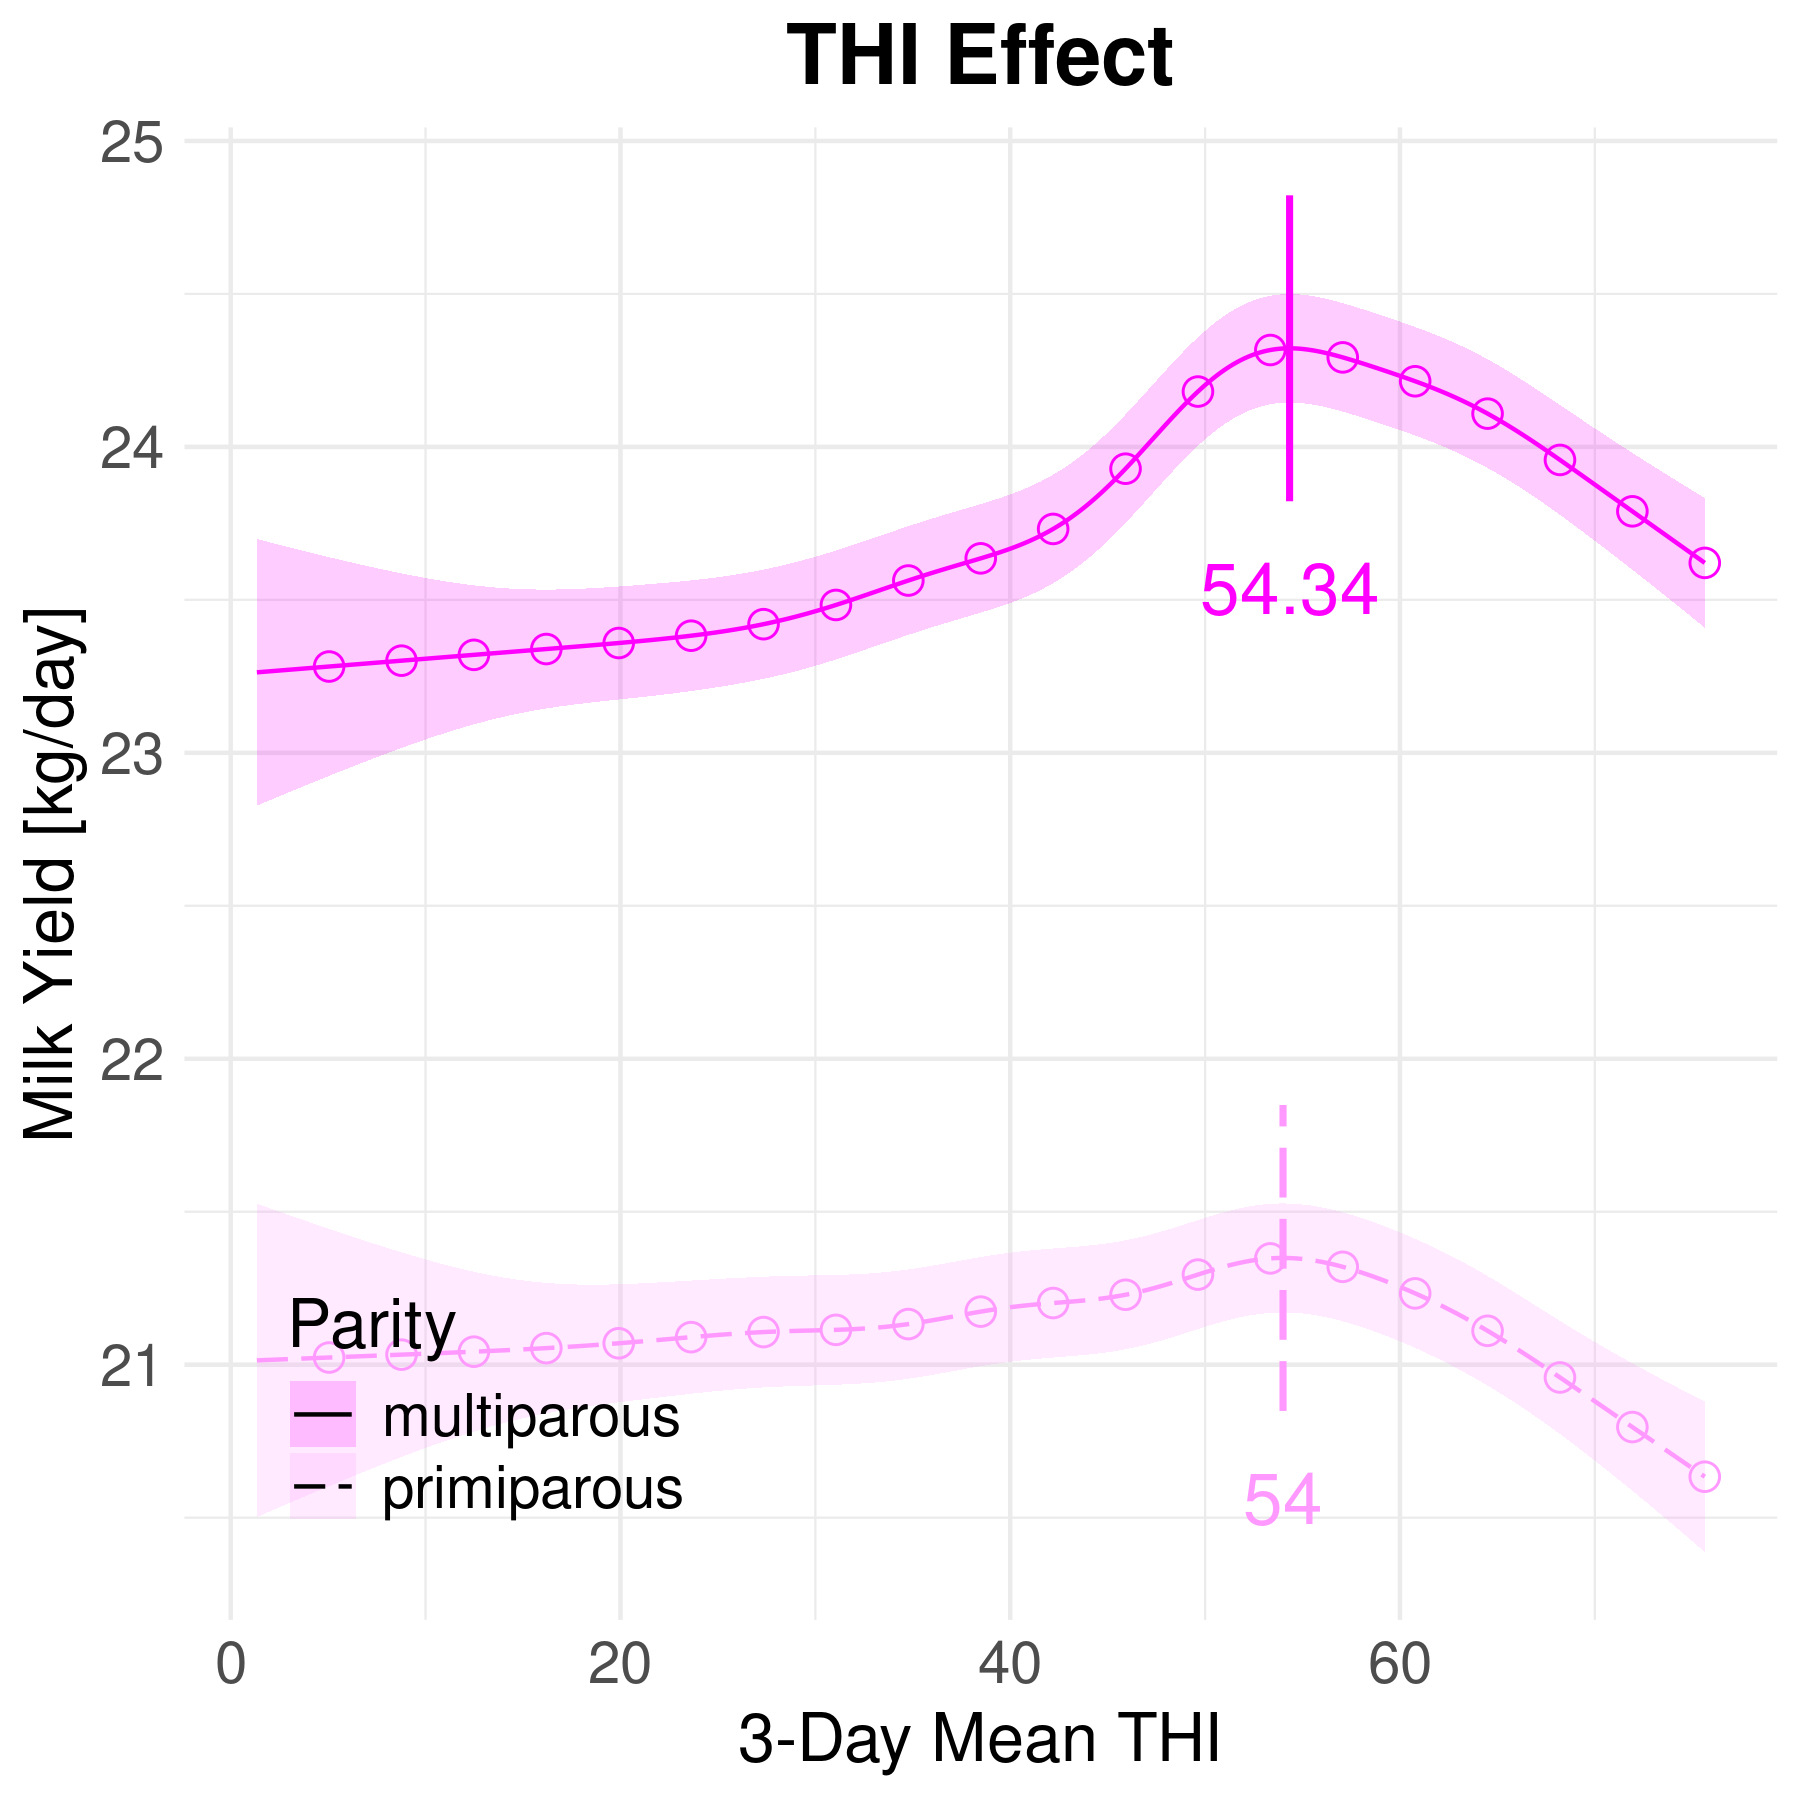
\includegraphics[width=\textwidth]{thesis/figures/models/milk/before2010/sf_milk_before2010/sf_milk_before2010_marginal_thi_milk_combined.png}
    \end{subfigure}
    \hspace{0.05\textwidth} % Optional space between the figures
    \begin{subfigure}[b]{0.45\textwidth}
        \centering
        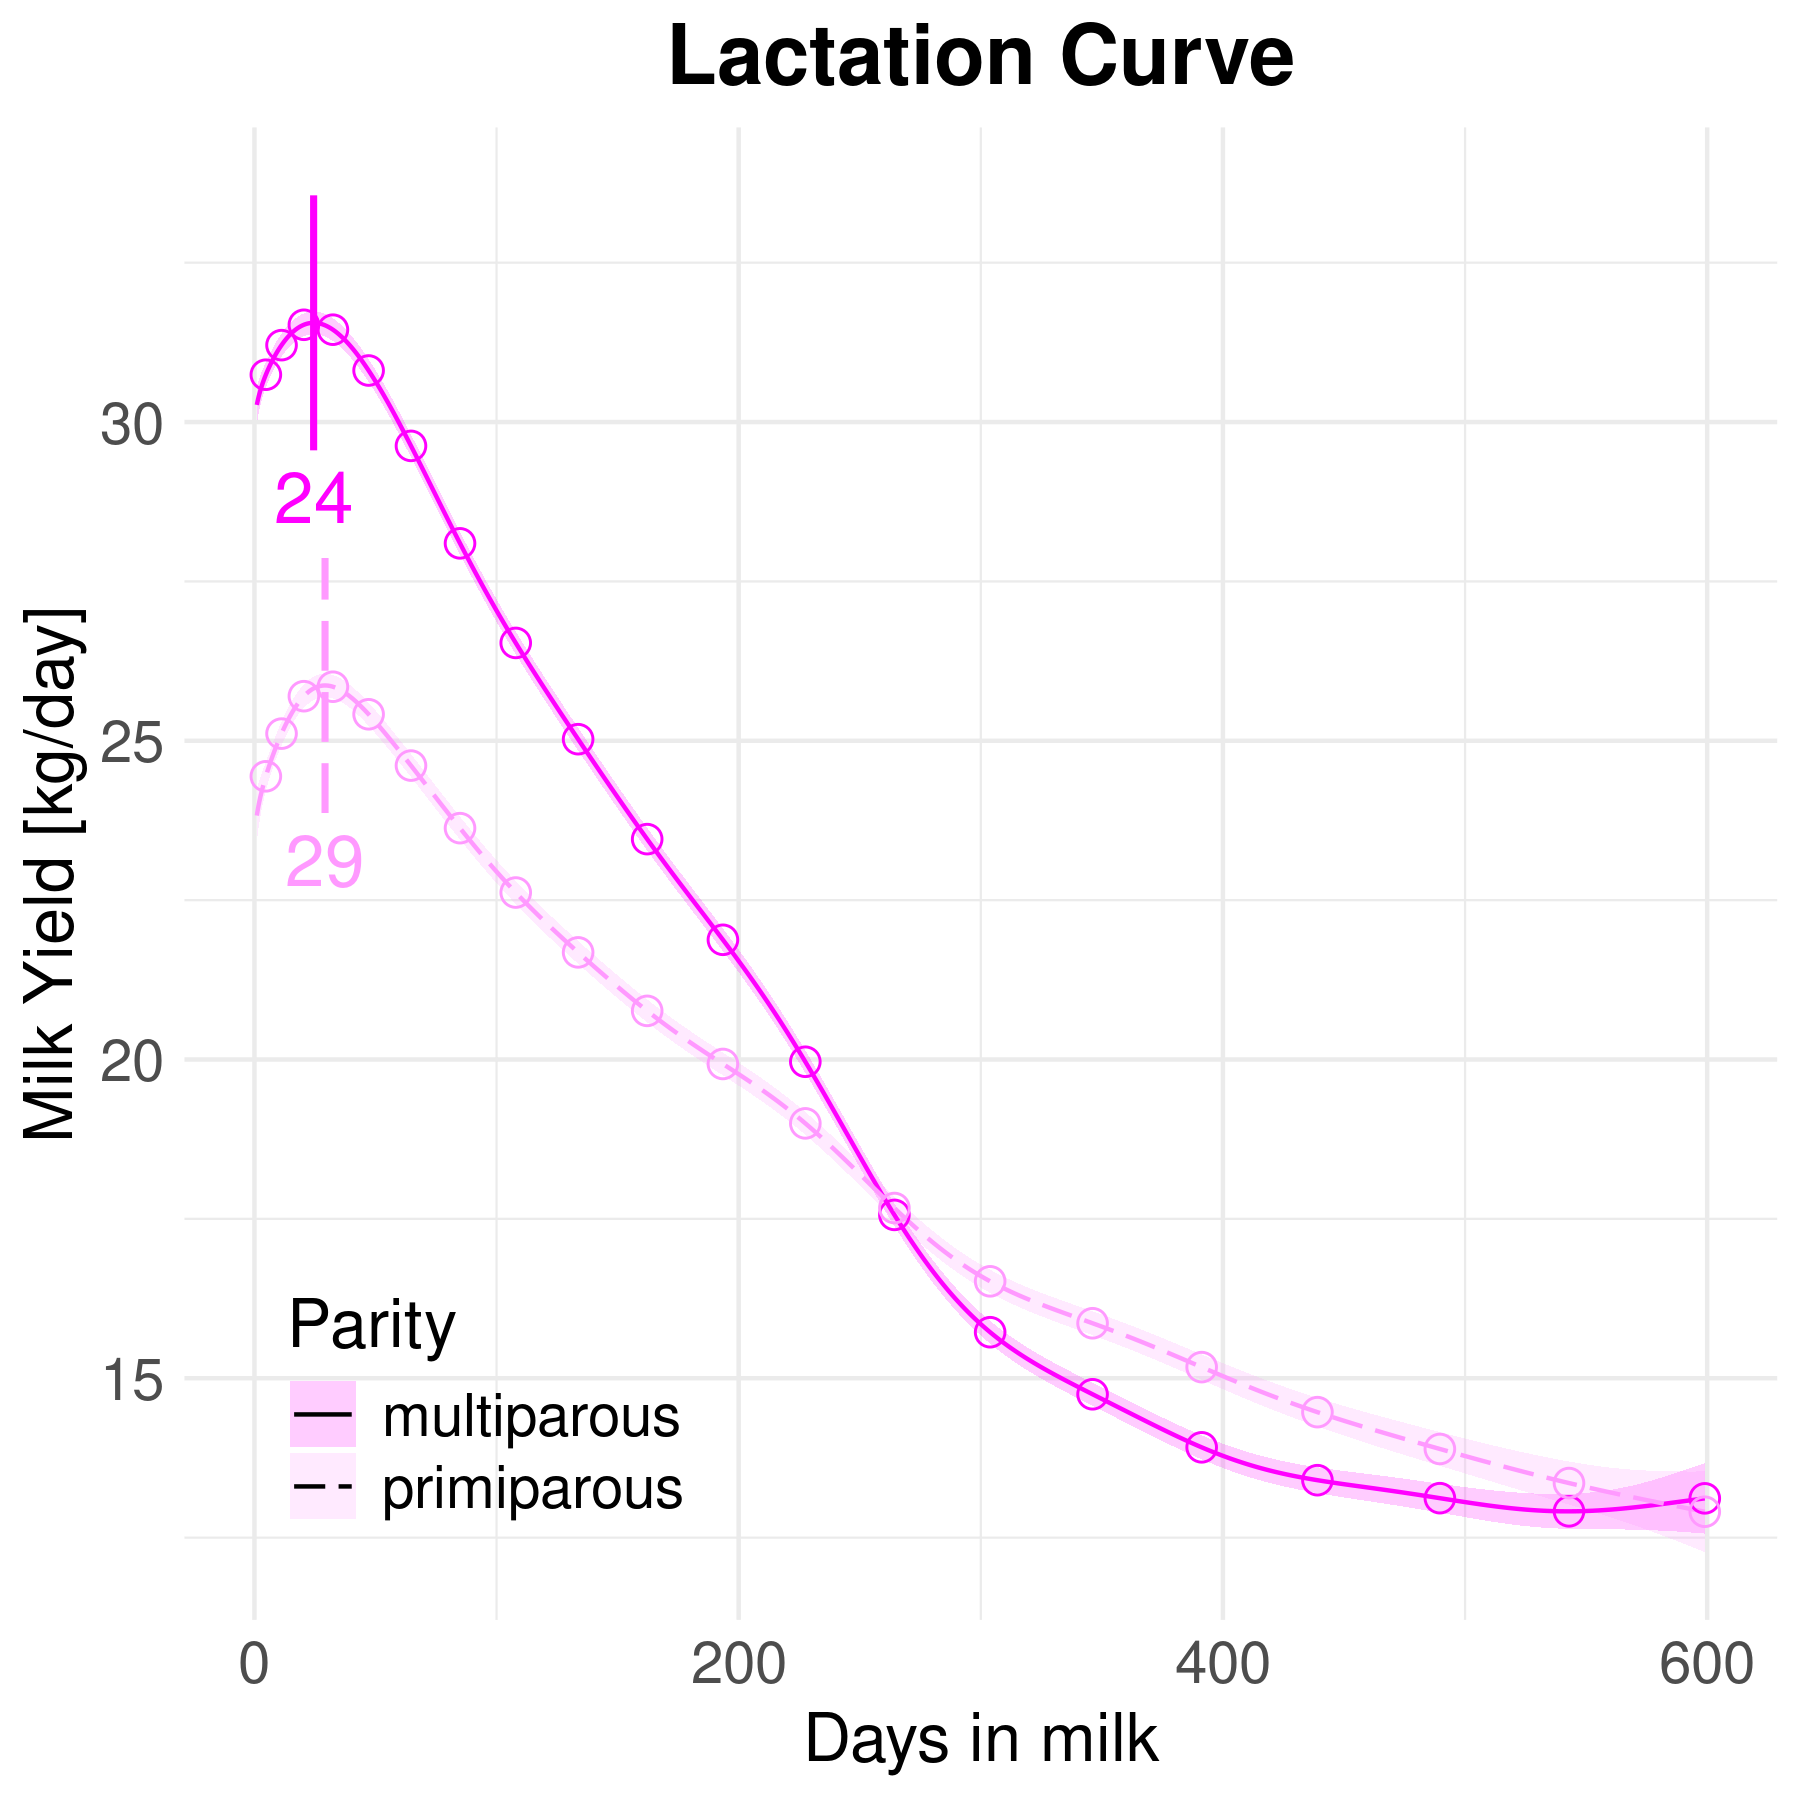
\includegraphics[width=\textwidth]{thesis/figures/models/milk/before2010/sf_milk_before2010/sf_milk_before2010_marginal_dim_milk_combined.png}
    \end{subfigure}
    \begin{subfigure}[b]{0.45\textwidth}
        \centering
        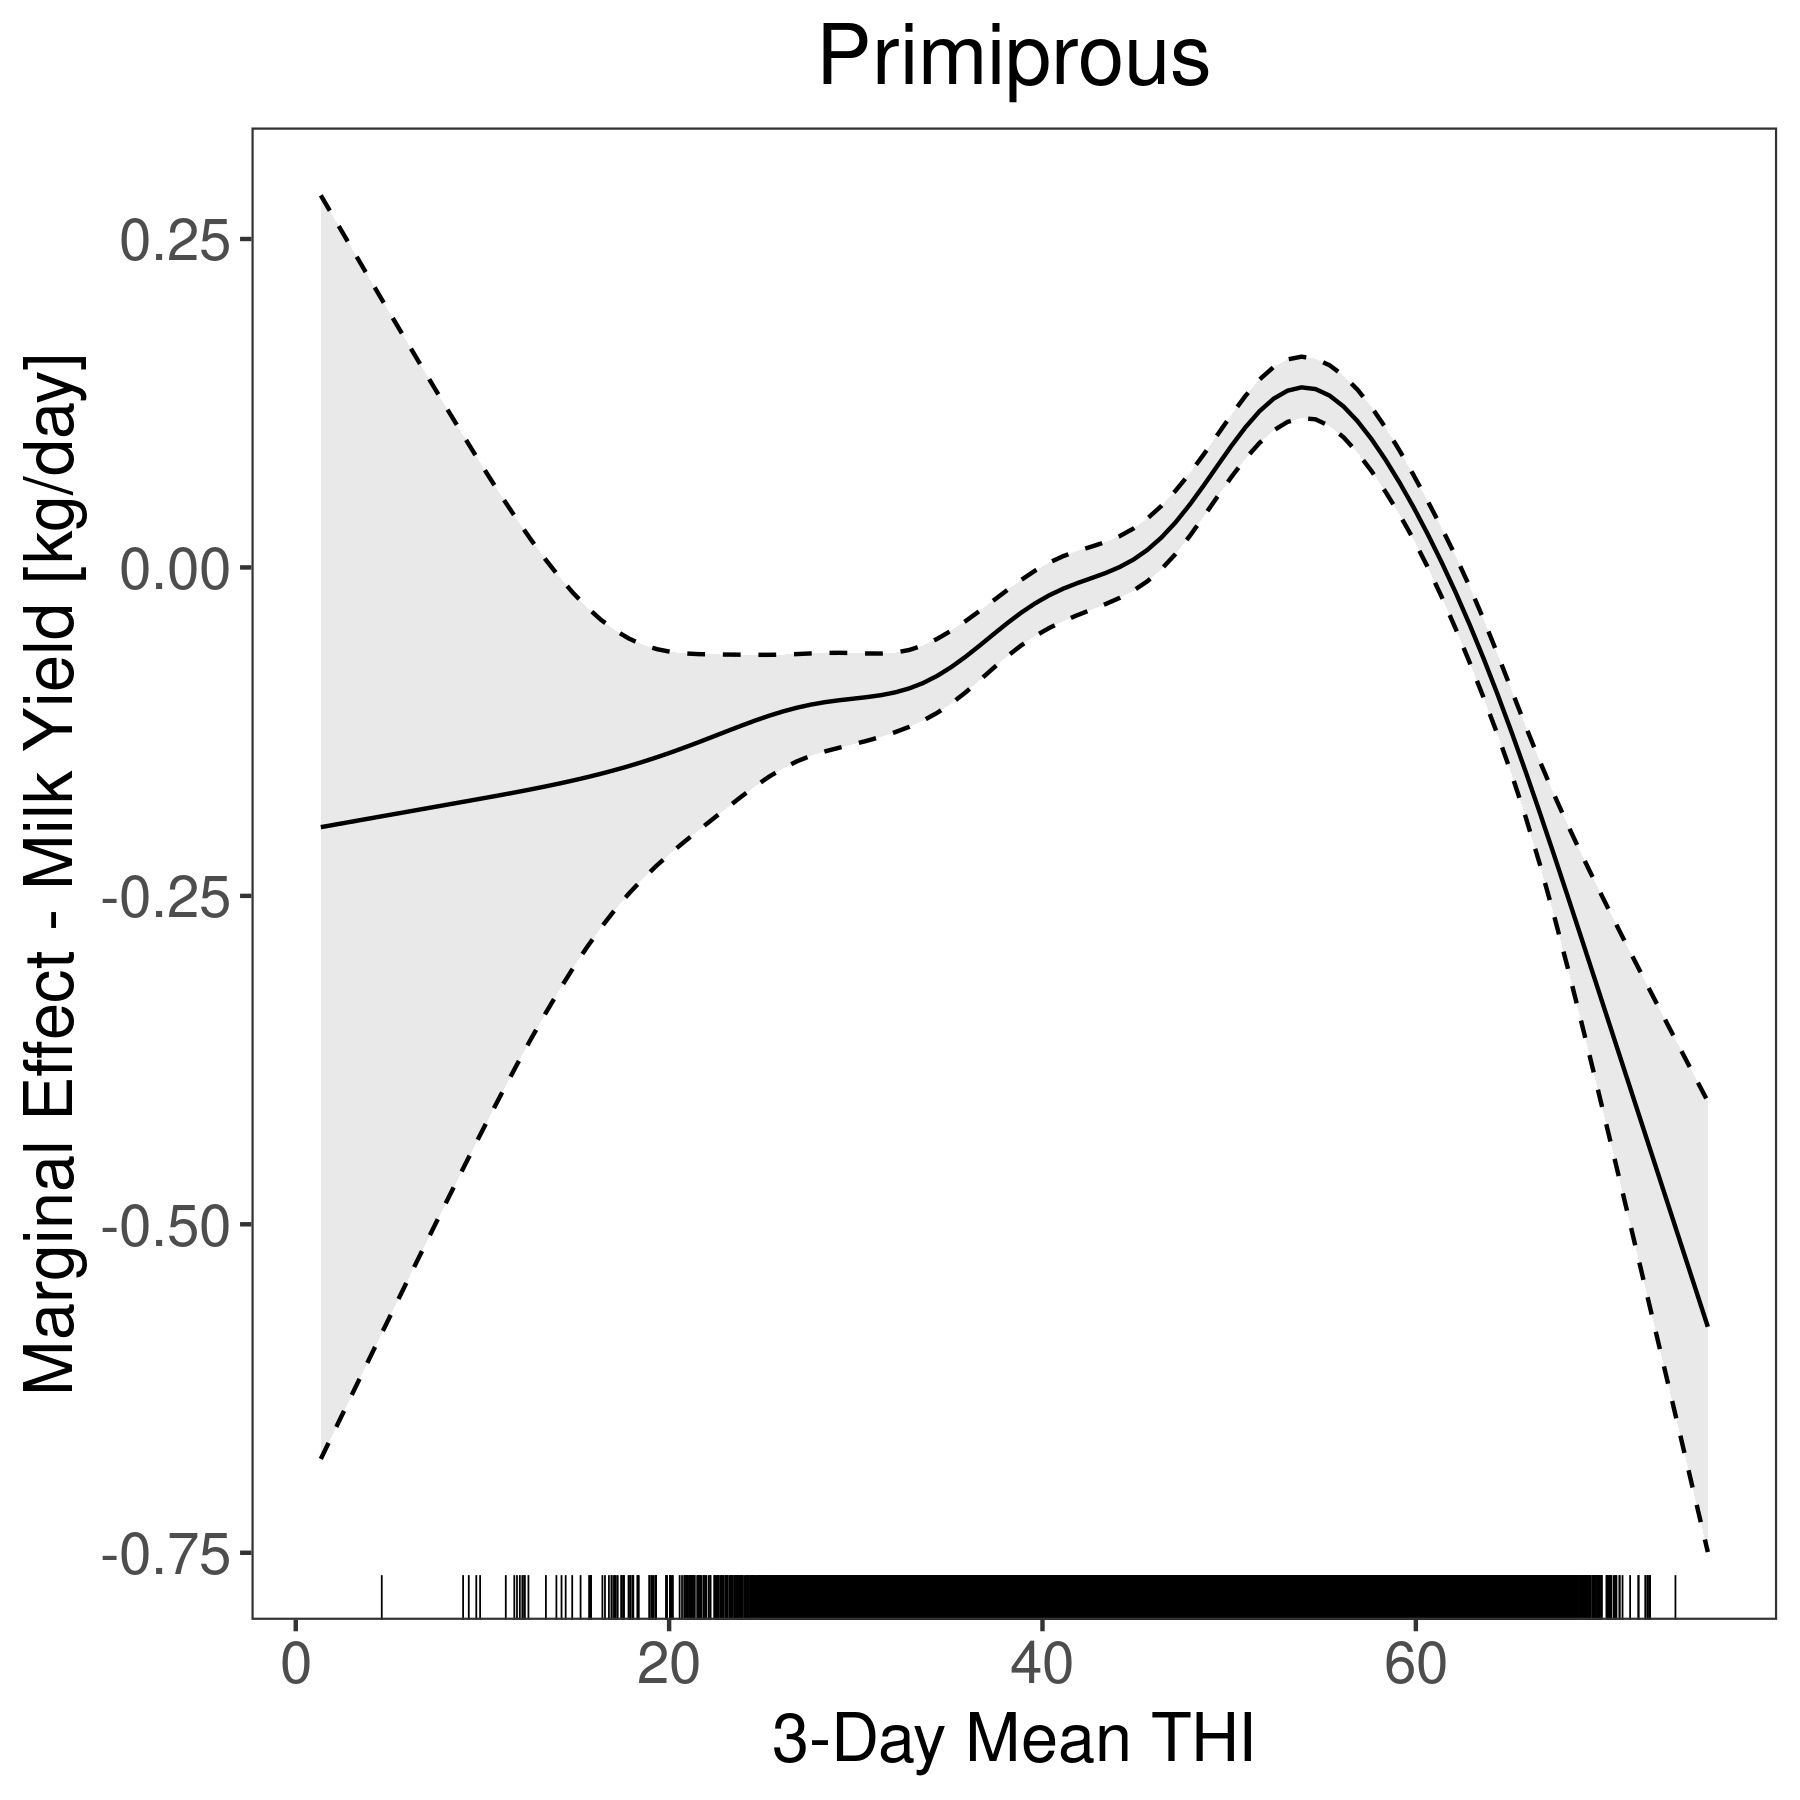
\includegraphics[width=\textwidth]{thesis/figures/models/milk/before2010/sf_milk_before2010/sf_milk_before2010_marginal_thi_milk_primi.png}
    \end{subfigure}
    \hspace{0.05\textwidth} % Optional space between the figures
    \begin{subfigure}[b]{0.45\textwidth}
        \centering
        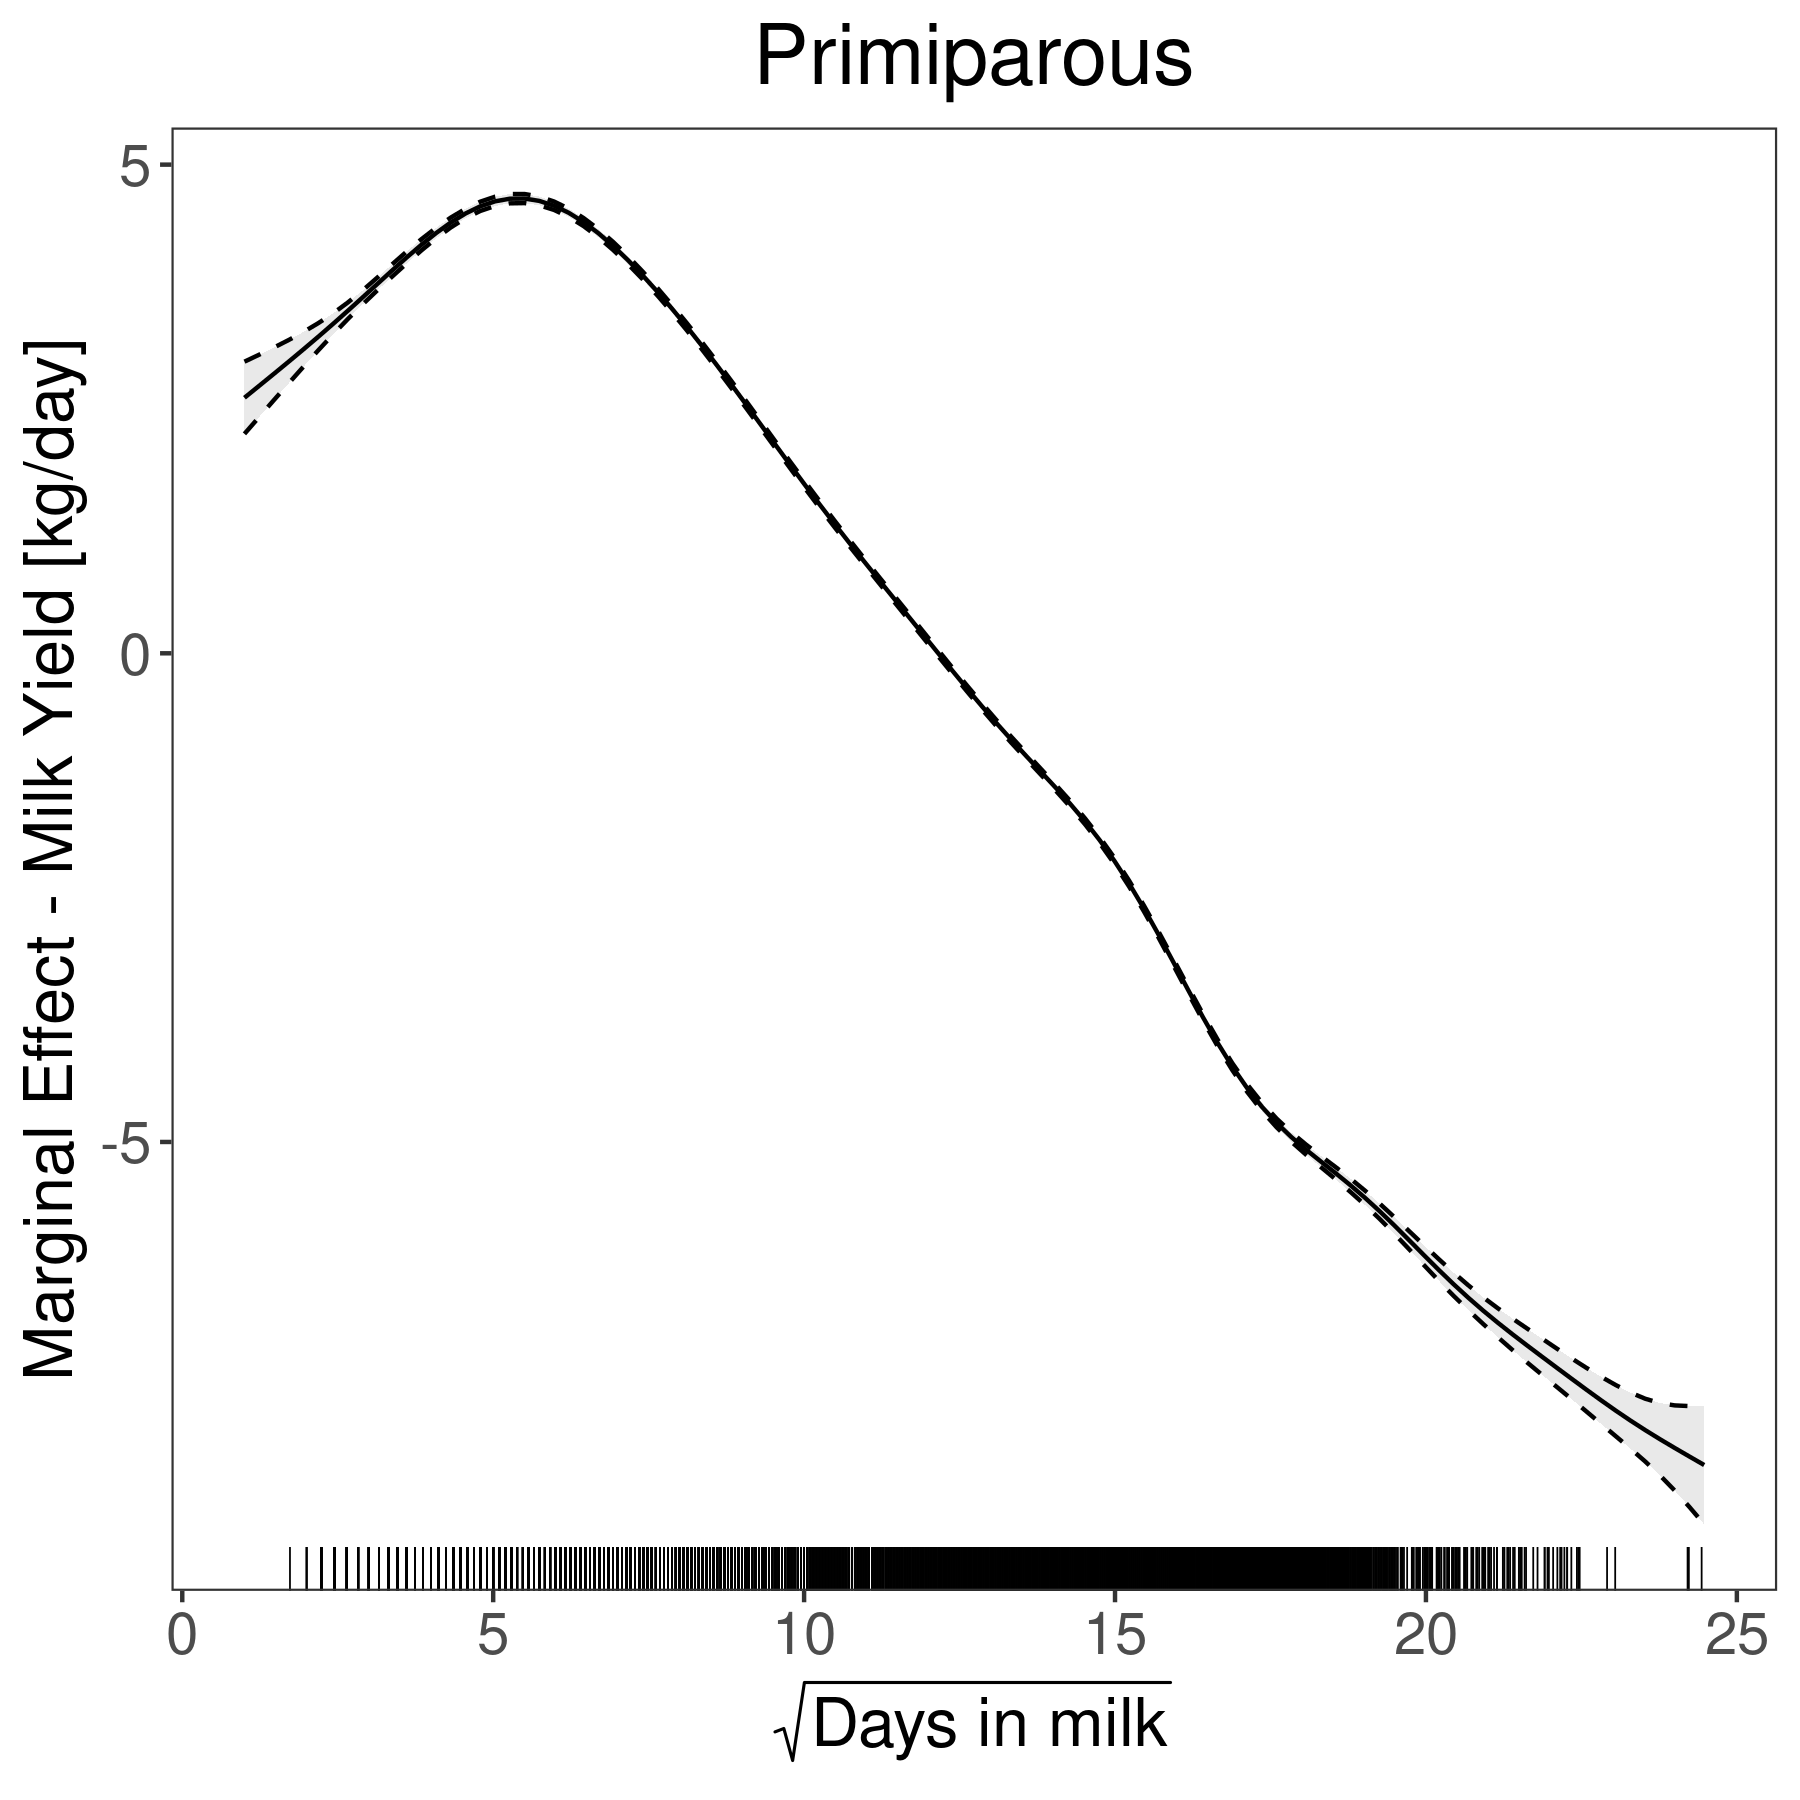
\includegraphics[width=\textwidth]{thesis/figures/models/milk/before2010/sf_milk_before2010/sf_milk_before2010_marginal_dim_milk_primi.png}
    \end{subfigure}
    \begin{subfigure}[b]{0.45\textwidth}
        \centering
        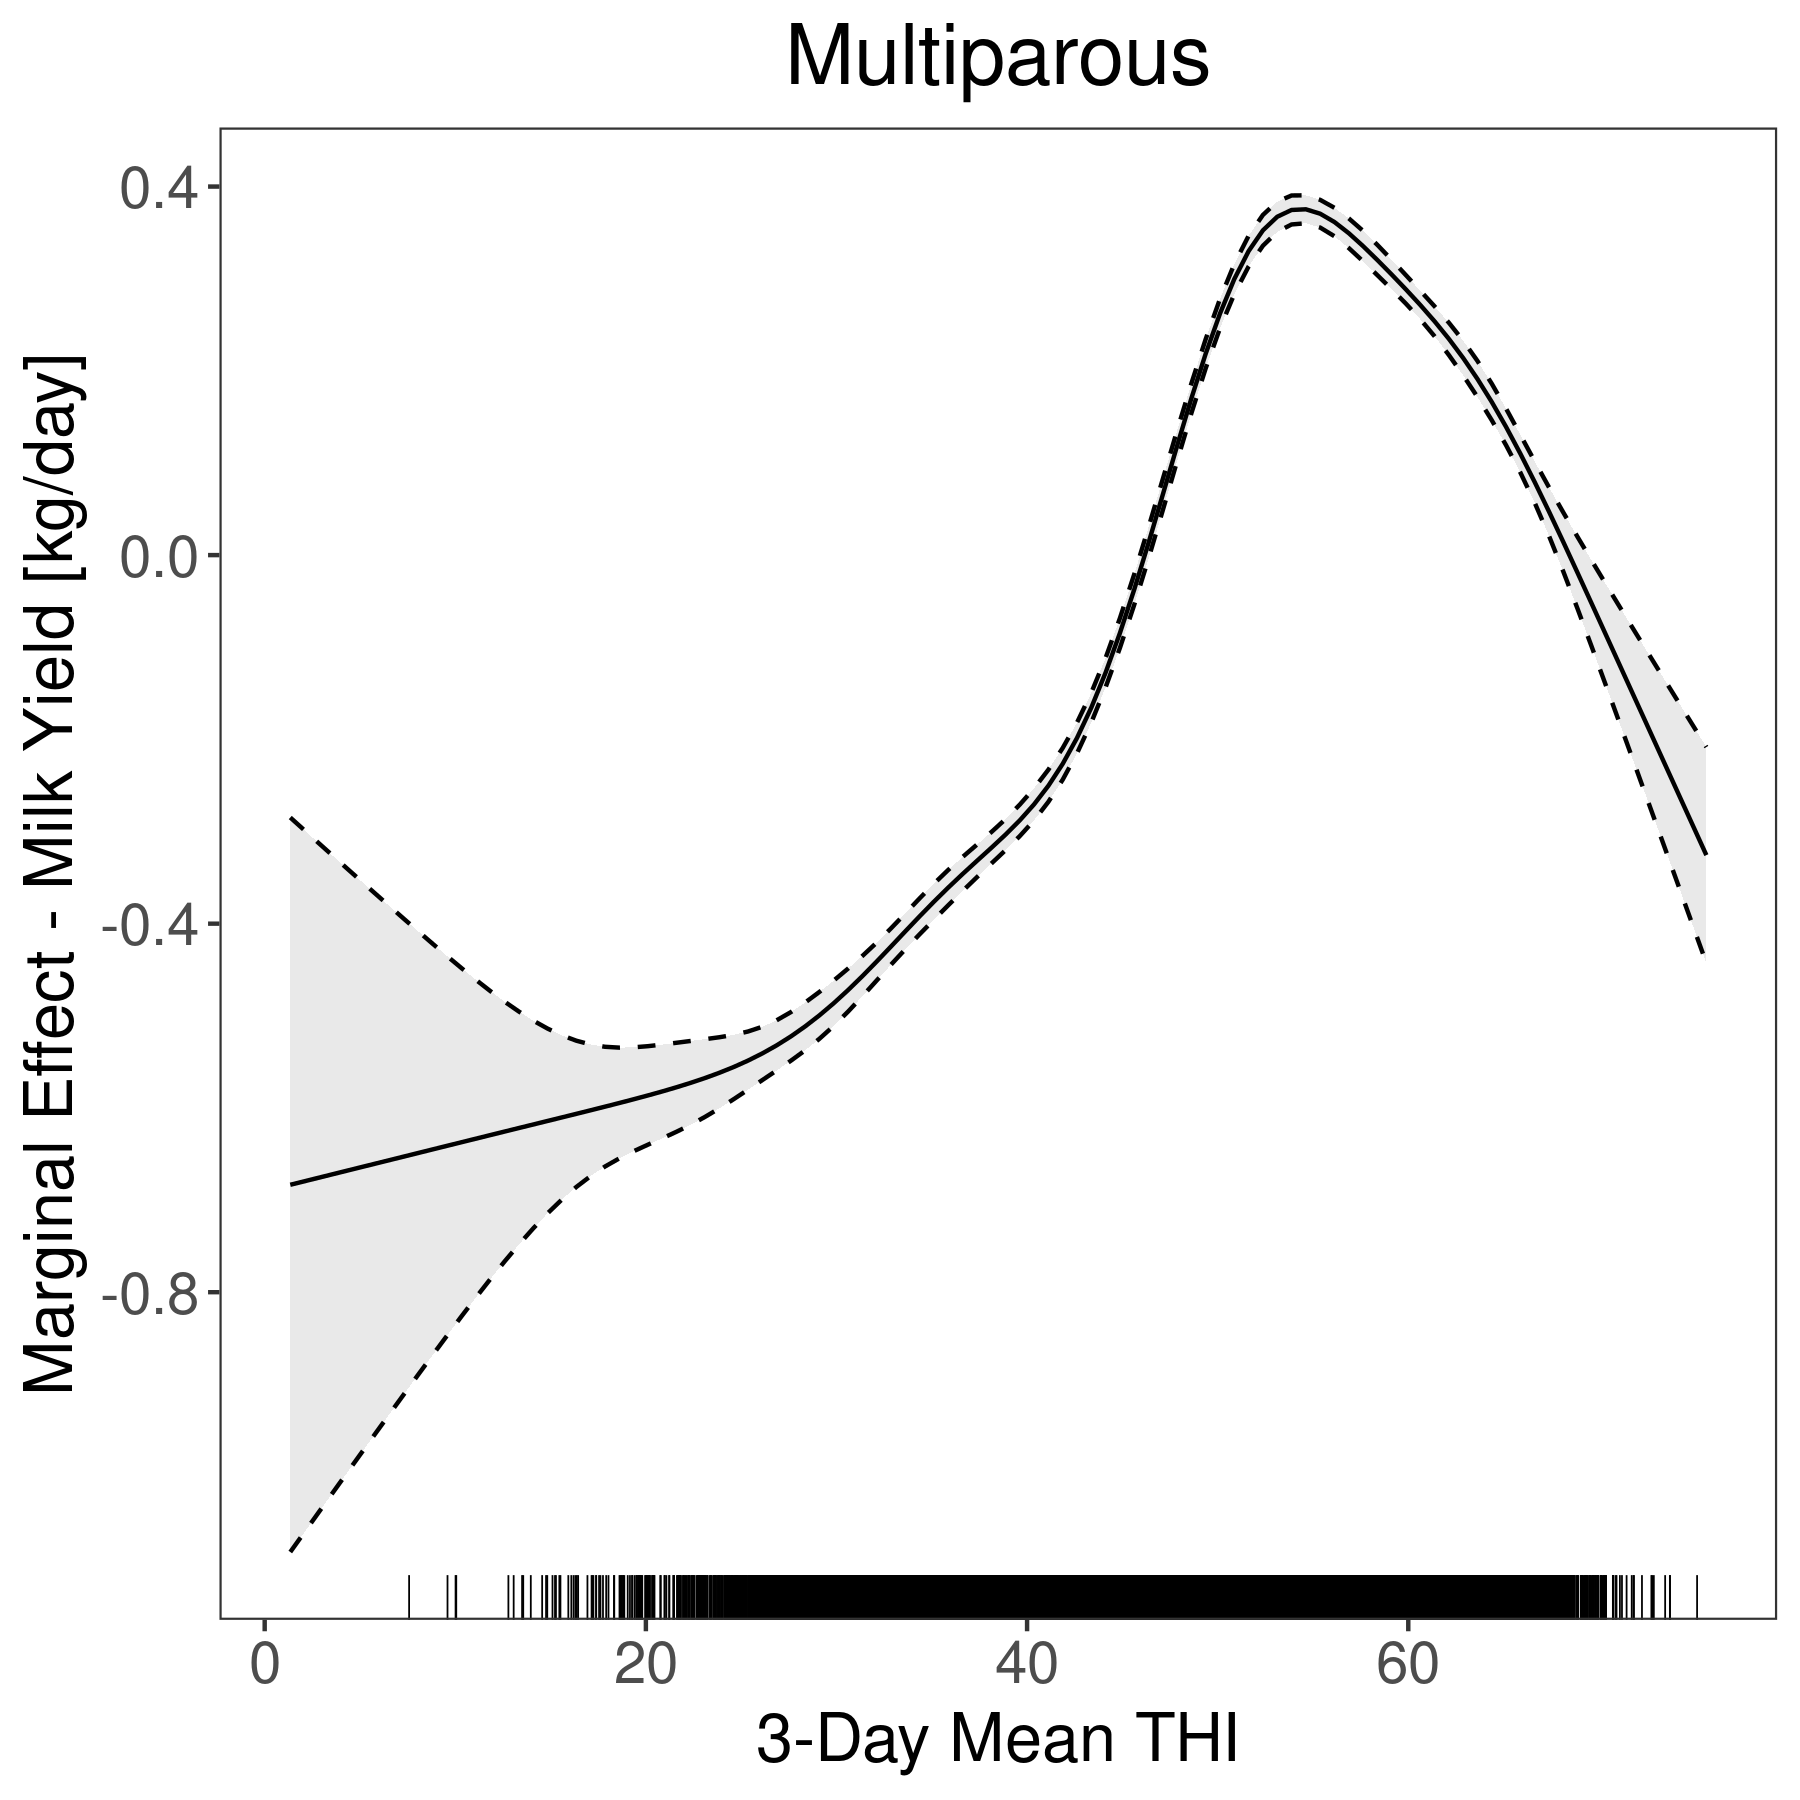
\includegraphics[width=\textwidth]{thesis/figures/models/milk/before2010/sf_milk_before2010/sf_milk_before2010_marginal_thi_milk_multi.png}
    \end{subfigure}
    \hspace{0.05\textwidth} % Optional space between the figures
    \begin{subfigure}[b]{0.45\textwidth}
        \centering
        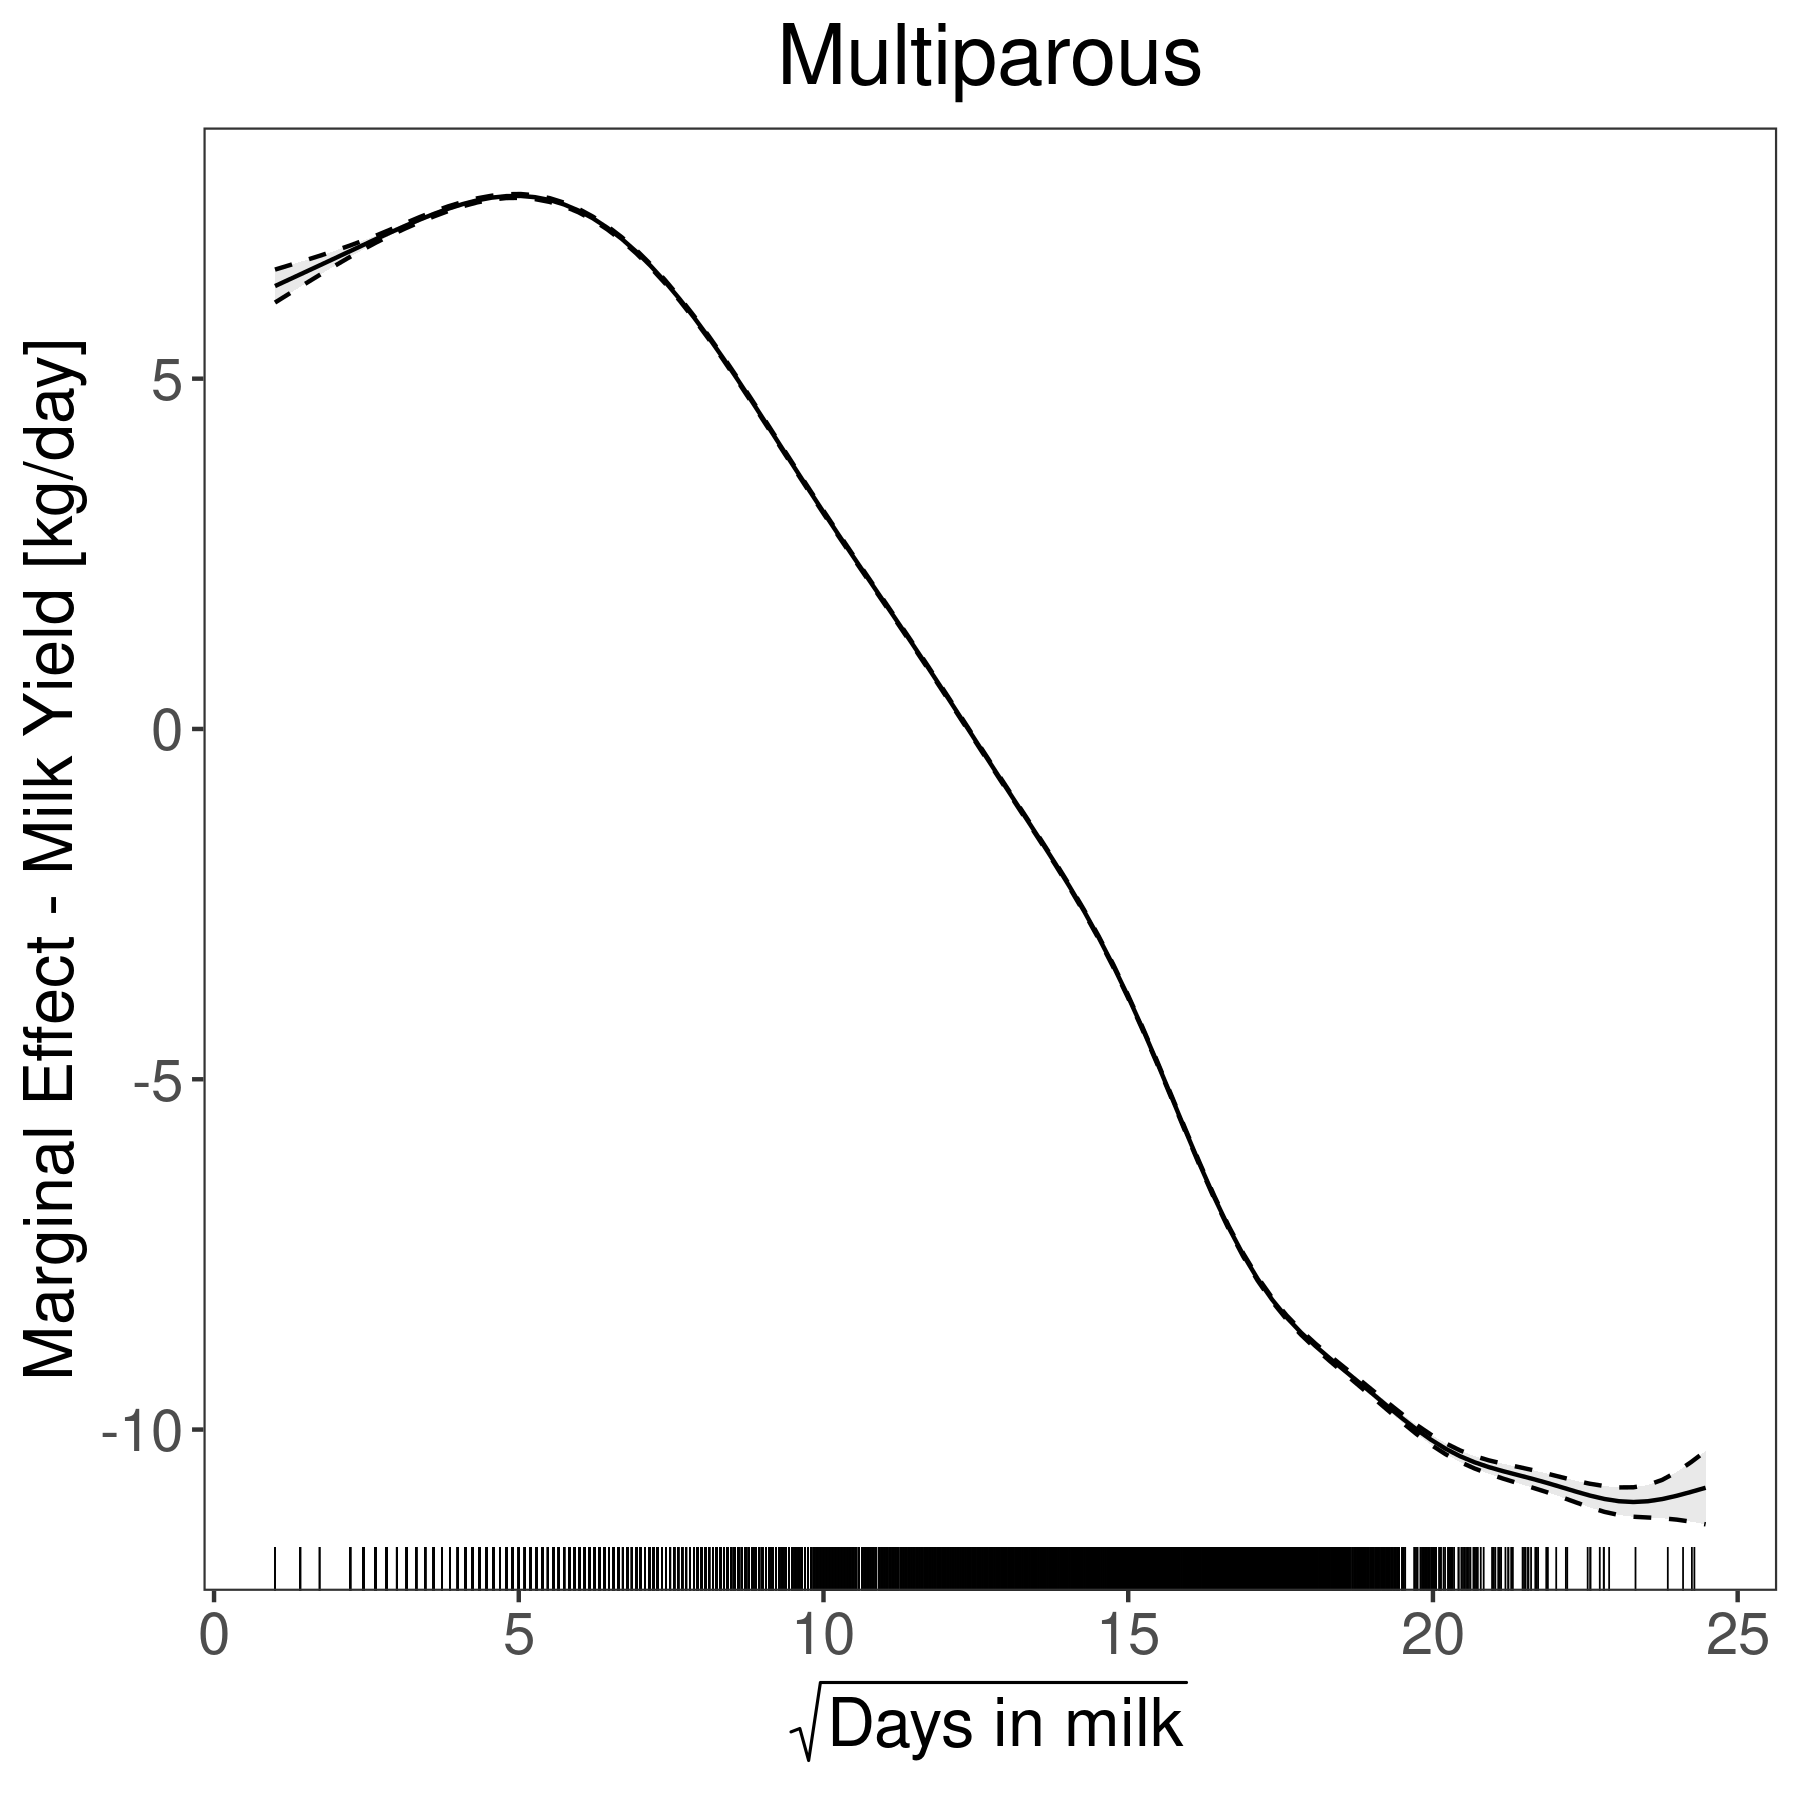
\includegraphics[width=\textwidth]{thesis/figures/models/milk/before2010/sf_milk_before2010/sf_milk_before2010_marginal_dim_milk_multi.png}
    \end{subfigure}
    \caption[]{Swiss Fleckvieh: Milk Yield - 1984 - 2010 - THI Effect and Lactation Curve}
    \label{fig:main}
\end{figure}

\subsubsection{Split Period: 2010 - 2023}\label{model:sf_milk_after}

\paragraph{Model Summary} \quad \\

    \begin{table}[H]
    \centering
    \begin{tabular}{lrrrr}
    \textbf{A. parametric coefficients} & Estimate & Std. Error & t-value & p-value \\ 
       \hline
       \hline
      (Intercept) & 21.7530 & 0.2595 & 83.8176 & $<$ 0.0001 \\ 
      parityprimiparous & -3.3595 & 0.0149 & -224.7296 & $<$ 0.0001 \\ 
      year2012 & -0.1631 & 0.3056 & -0.5337 & 0.5936 \\ 
      year2013 & -0.3339 & 0.2926 & -1.1414 & 0.2537 \\ 
      year2014 & 0.2384 & 0.2906 & 0.8203 & 0.4121 \\ 
      year2015 & 0.4961 & 0.2957 & 1.6777 & 0.0934 \\ 
      year2016 & 0.8626 & 0.2984 & 2.8910 & 0.0038 \\ 
      year2017 & 1.2313 & 0.2939 & 4.1894 & $<$ 0.0001 \\ 
      year2018 & 1.6165 & 0.2967 & 5.4488 & $<$ 0.0001 \\ 
      year2019 & 1.7695 & 0.2943 & 6.0121 & $<$ 0.0001 \\ 
      year2020 & 2.0975 & 0.3029 & 6.9248 & $<$ 0.0001 \\ 
      year2021 & 2.3398 & 0.2847 & 8.2183 & $<$ 0.0001 \\ 
      year2022 & 2.1729 & 0.3008 & 7.2243 & $<$ 0.0001 \\ 
      year2023 & 2.3855 & 0.2954 & 8.0764 & $<$ 0.0001 \\ 
       \hline
    \textbf{B. smooth terms} & edf & Ref.df & F-value & p-value \\ 
    \hline
    \hline
      s(thi\_mean\_t0\_3d):paritymultiparous & 8.1653 & 8.1653 & 699.8806 & $<$ 0.0001 \\ 
      s(thi\_mean\_t0\_3d):parityprimiparous & 6.5967 & 6.5967 & 37.1793 & $<$ 0.0001 \\ 
      s(days\_in\_milk\_t):paritymultiparous & 14.5202 & 14.5202 & 113726.1561 & $<$ 0.0001 \\ 
      s(days\_in\_milk\_t):parityprimiparous & 13.5621 & 13.5621 & 11375.9787 & $<$ 0.0001 \\  
       \hline
    \end{tabular}
    \caption[]{Swiss Fleckvieh: Milk Yield - 2011-2023 - GAMM model summary without random effect terms.}
    \end{table}

\newpage
\begin{table}[H]
\centering
\begin{tabular}
{l | r | r | r | r}
\textbf{Smooth Term Fixed Effect} & Est. & SE & z & p\\
\hline
\hline
s(thi\_mean\_t0\_3d):multiFx1 & 0.1716 & 0.0901 & 1.91 & 0.0568\\
s(thi\_mean\_t0\_3d):primiFx1 & -0.2638 & 0.1058 & -2.49 & 0.0126\\
s(days\_in\_milk\_):multiFx1 & 3.0173 & 0.4977 & 6.06 & $<$ 1e-08\\
s(days\_in\_milk\_):primiFx1 & 3.2102 & 0.6274 & 5.12 & $<$ 1e-06\\
\hline
\textbf{Variance Component} & Estimated $\sigma$ & & & \\
\hline
\hline
$\sigma_\alpha$ & 2.7938 & & & \\
$\sigma_\iota$ & 1.0653 & & & \\
$\sigma_\phi$ & 3.2540 & & & \\
s(thi\_mean\_t0\_3d):multi &  1.8095 & & & \\
s(days\_in\_milk\_):primi & 7.0409 & & & \\
s(days\_in\_milk\_):multi & 9.4413 & & & \\
s(thi\_mean\_t0\_3d):primi & 1.2895 & & & \\
Residual & 3.4929 & & & \\
\end{tabular}
\caption[]{Swiss Fleckvieh: Milk Yield - 2011-2023 - Mixed Model Summary - Smooth Terms and Random Effects.}
\end{table}



\paragraph{Model Diagnostics} \quad \\
\begin{figure}[H]
    \centering
    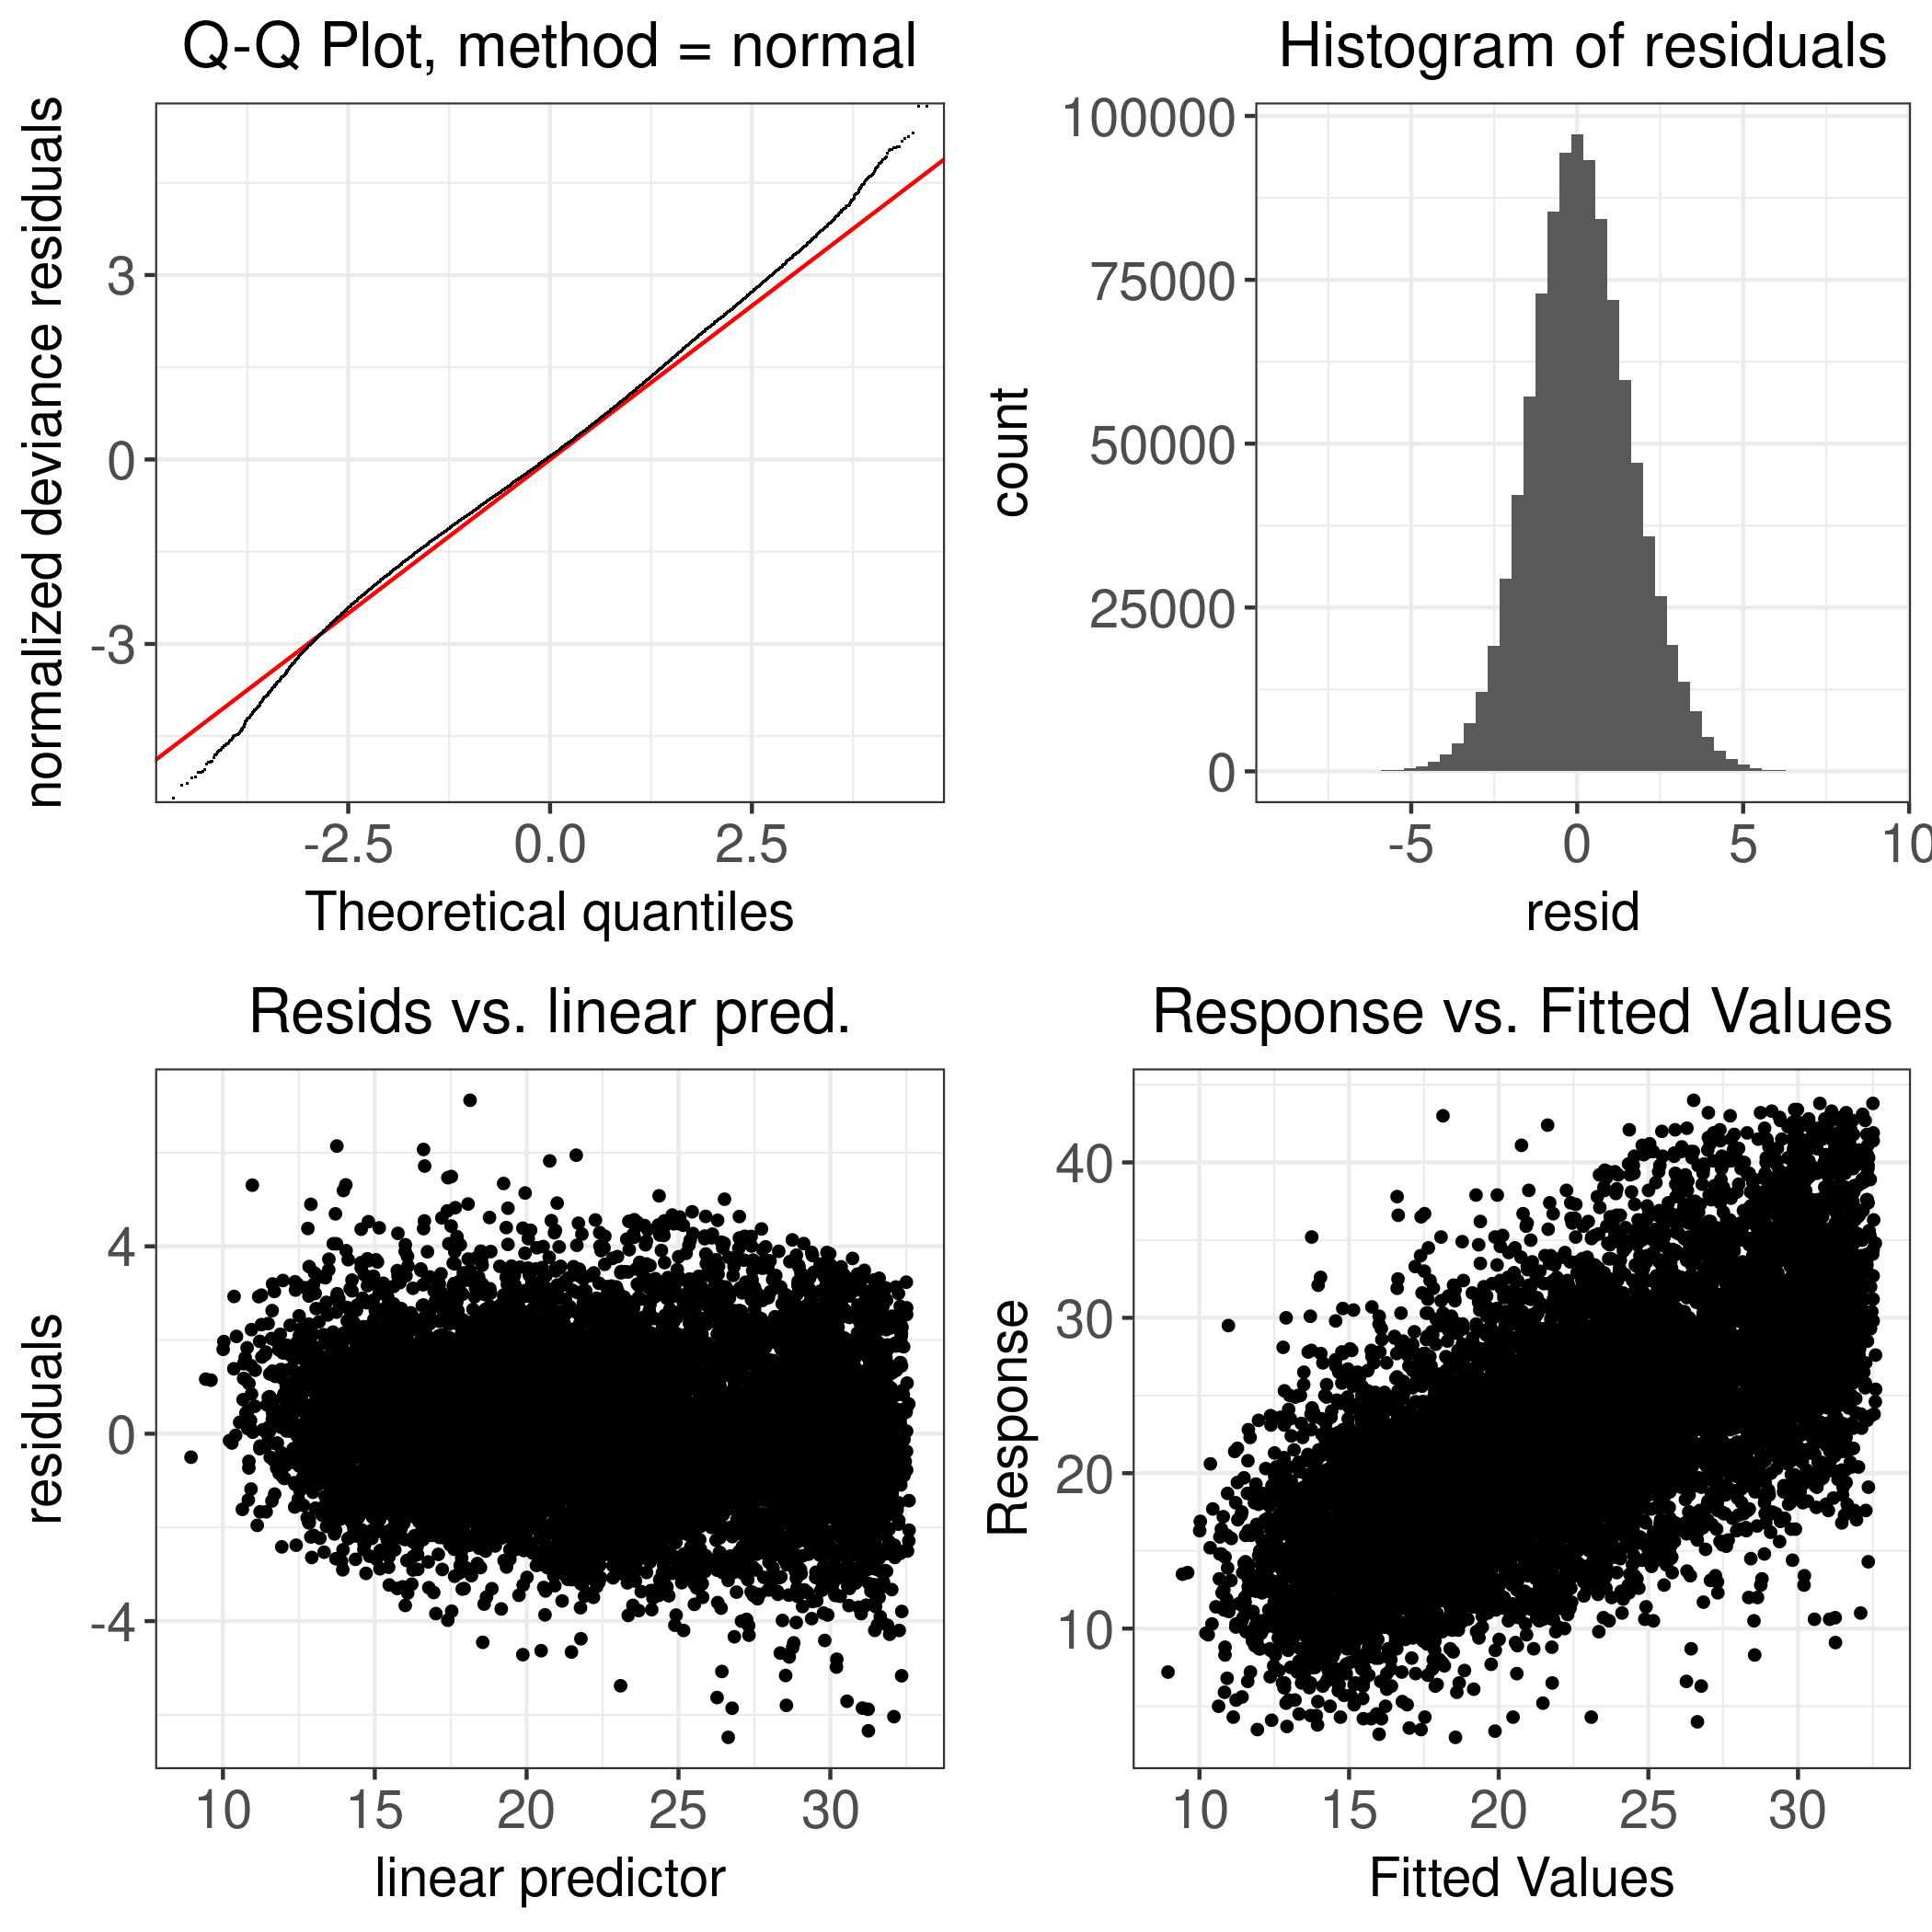
\includegraphics[width=0.6\textwidth]{thesis/figures/models/milk/after2010/sf_milk_after2010/sf_milk_after2010_diagnostics.png}
    \caption[]{Swiss Fleckvieh: Milk Yield - 2011-2023 - Diagnostic Plot}
\end{figure}

\newpage
\paragraph{THI Effect and Lactation Curve} \quad \\
\begin{figure}[H]
    \centering
    \begin{subfigure}[b]{0.45\textwidth}
        \centering
        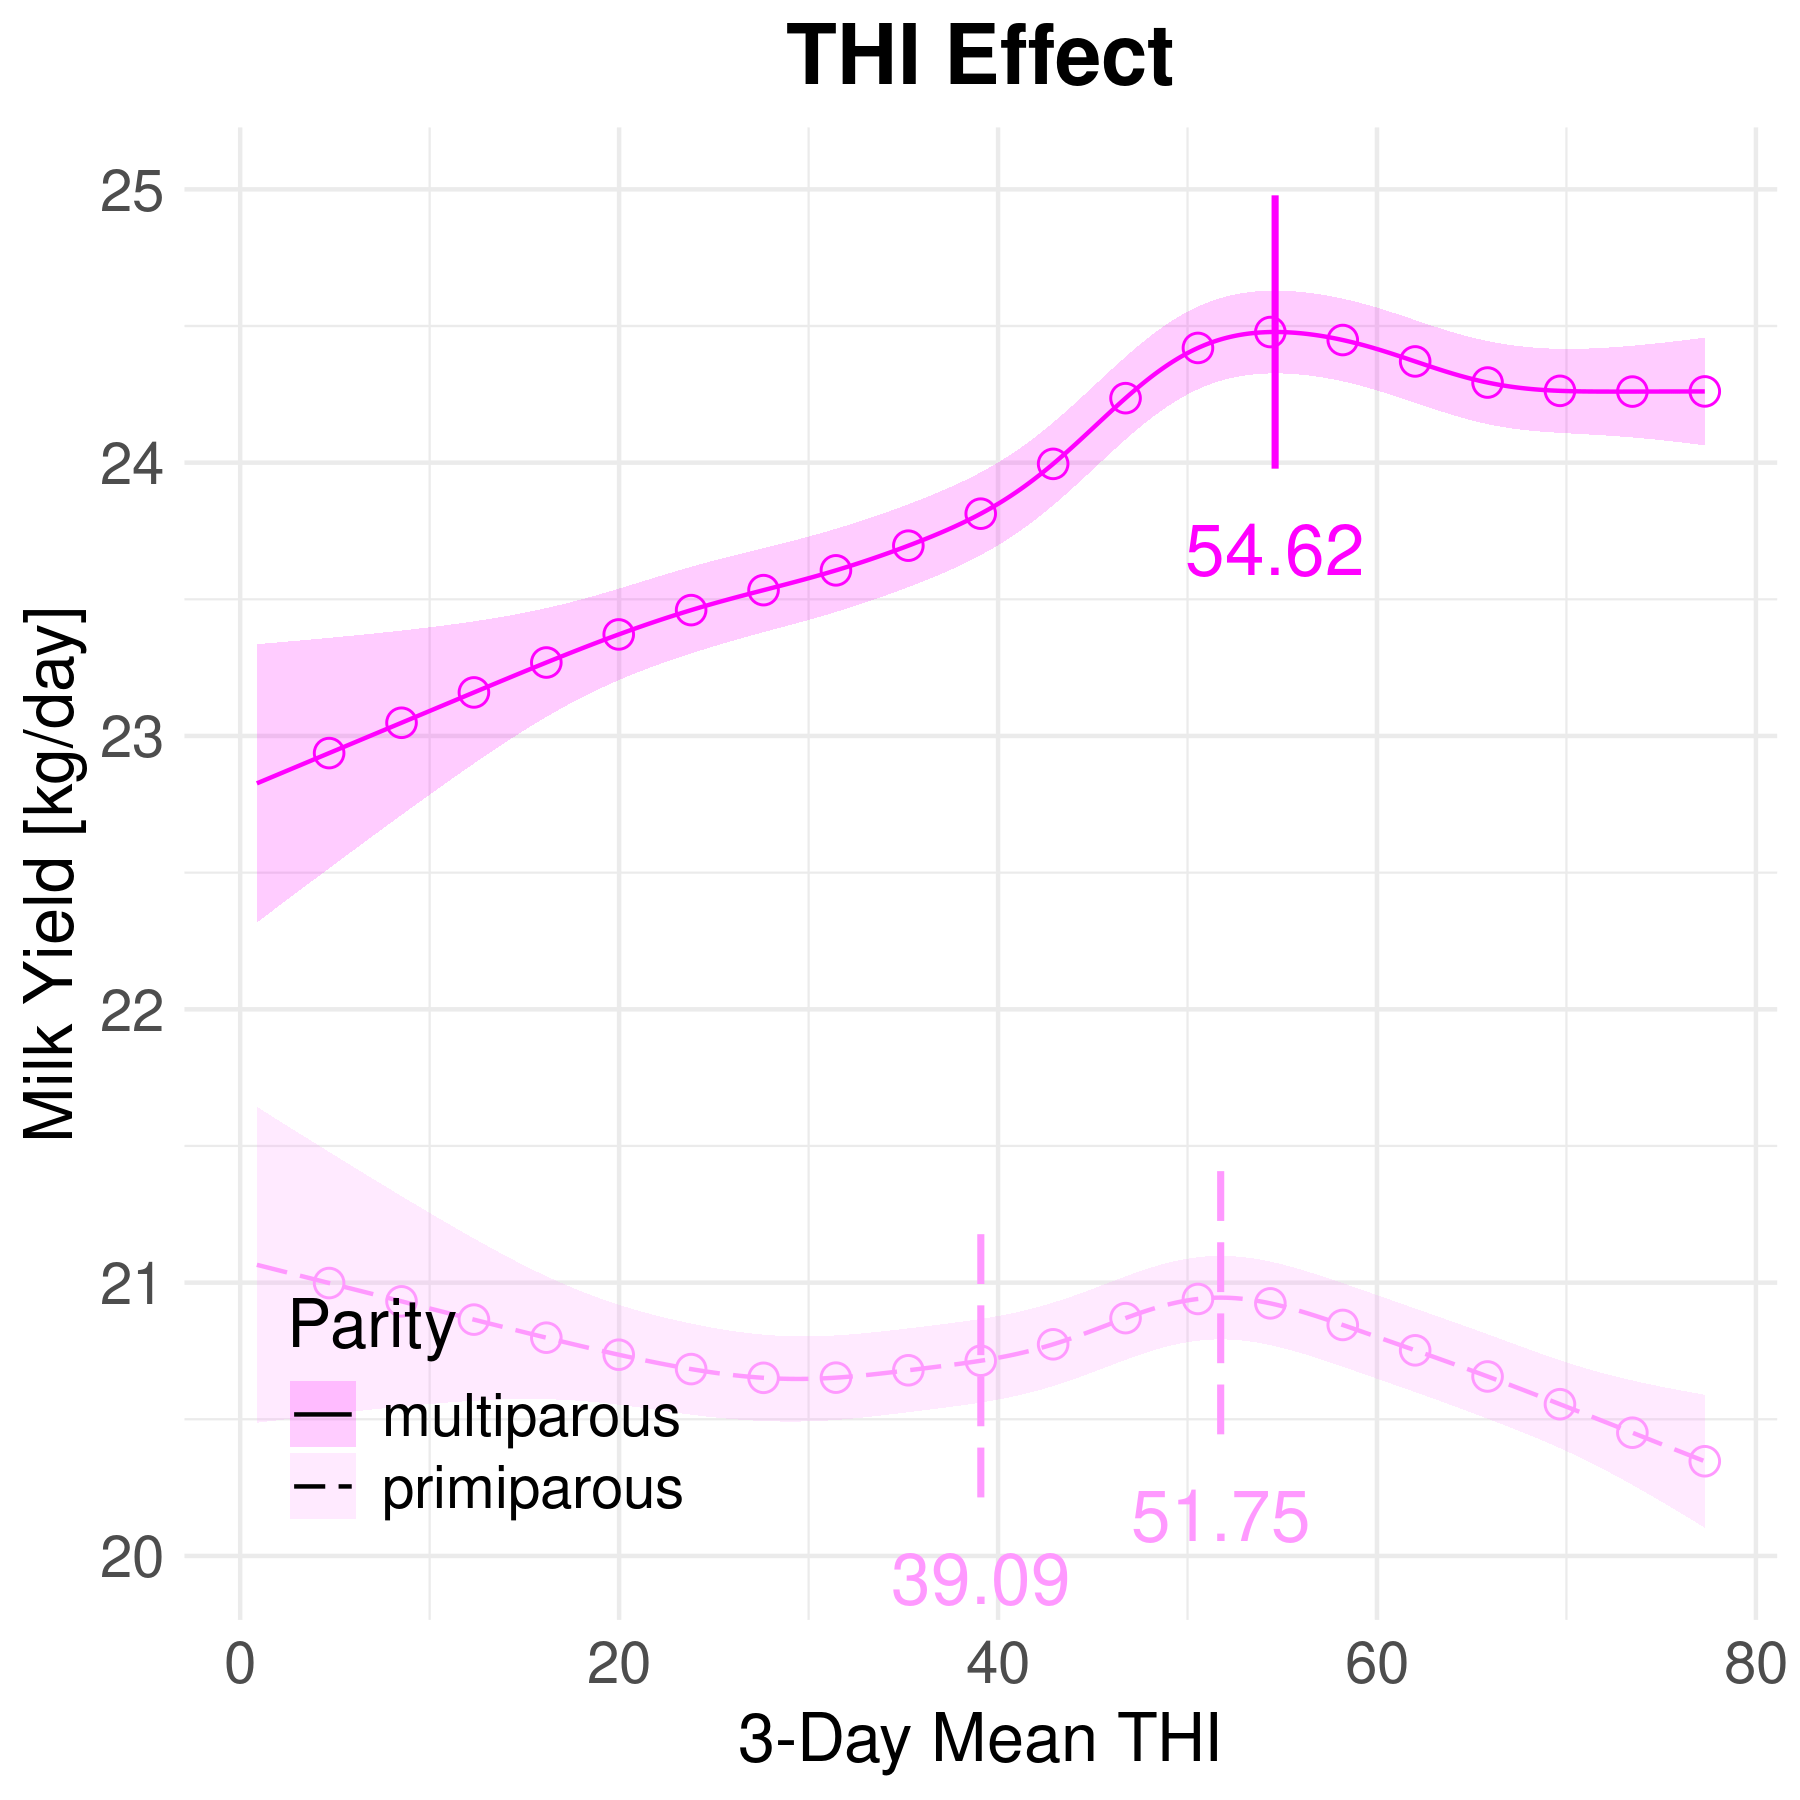
\includegraphics[width=\textwidth]{thesis/figures/models/milk/after2010/sf_milk_after2010/sf_milk_after2010_marginal_thi_milk_combined.png}
    \end{subfigure}
    \hspace{0.05\textwidth} % Optional space between the figures
    \begin{subfigure}[b]{0.45\textwidth}
        \centering
        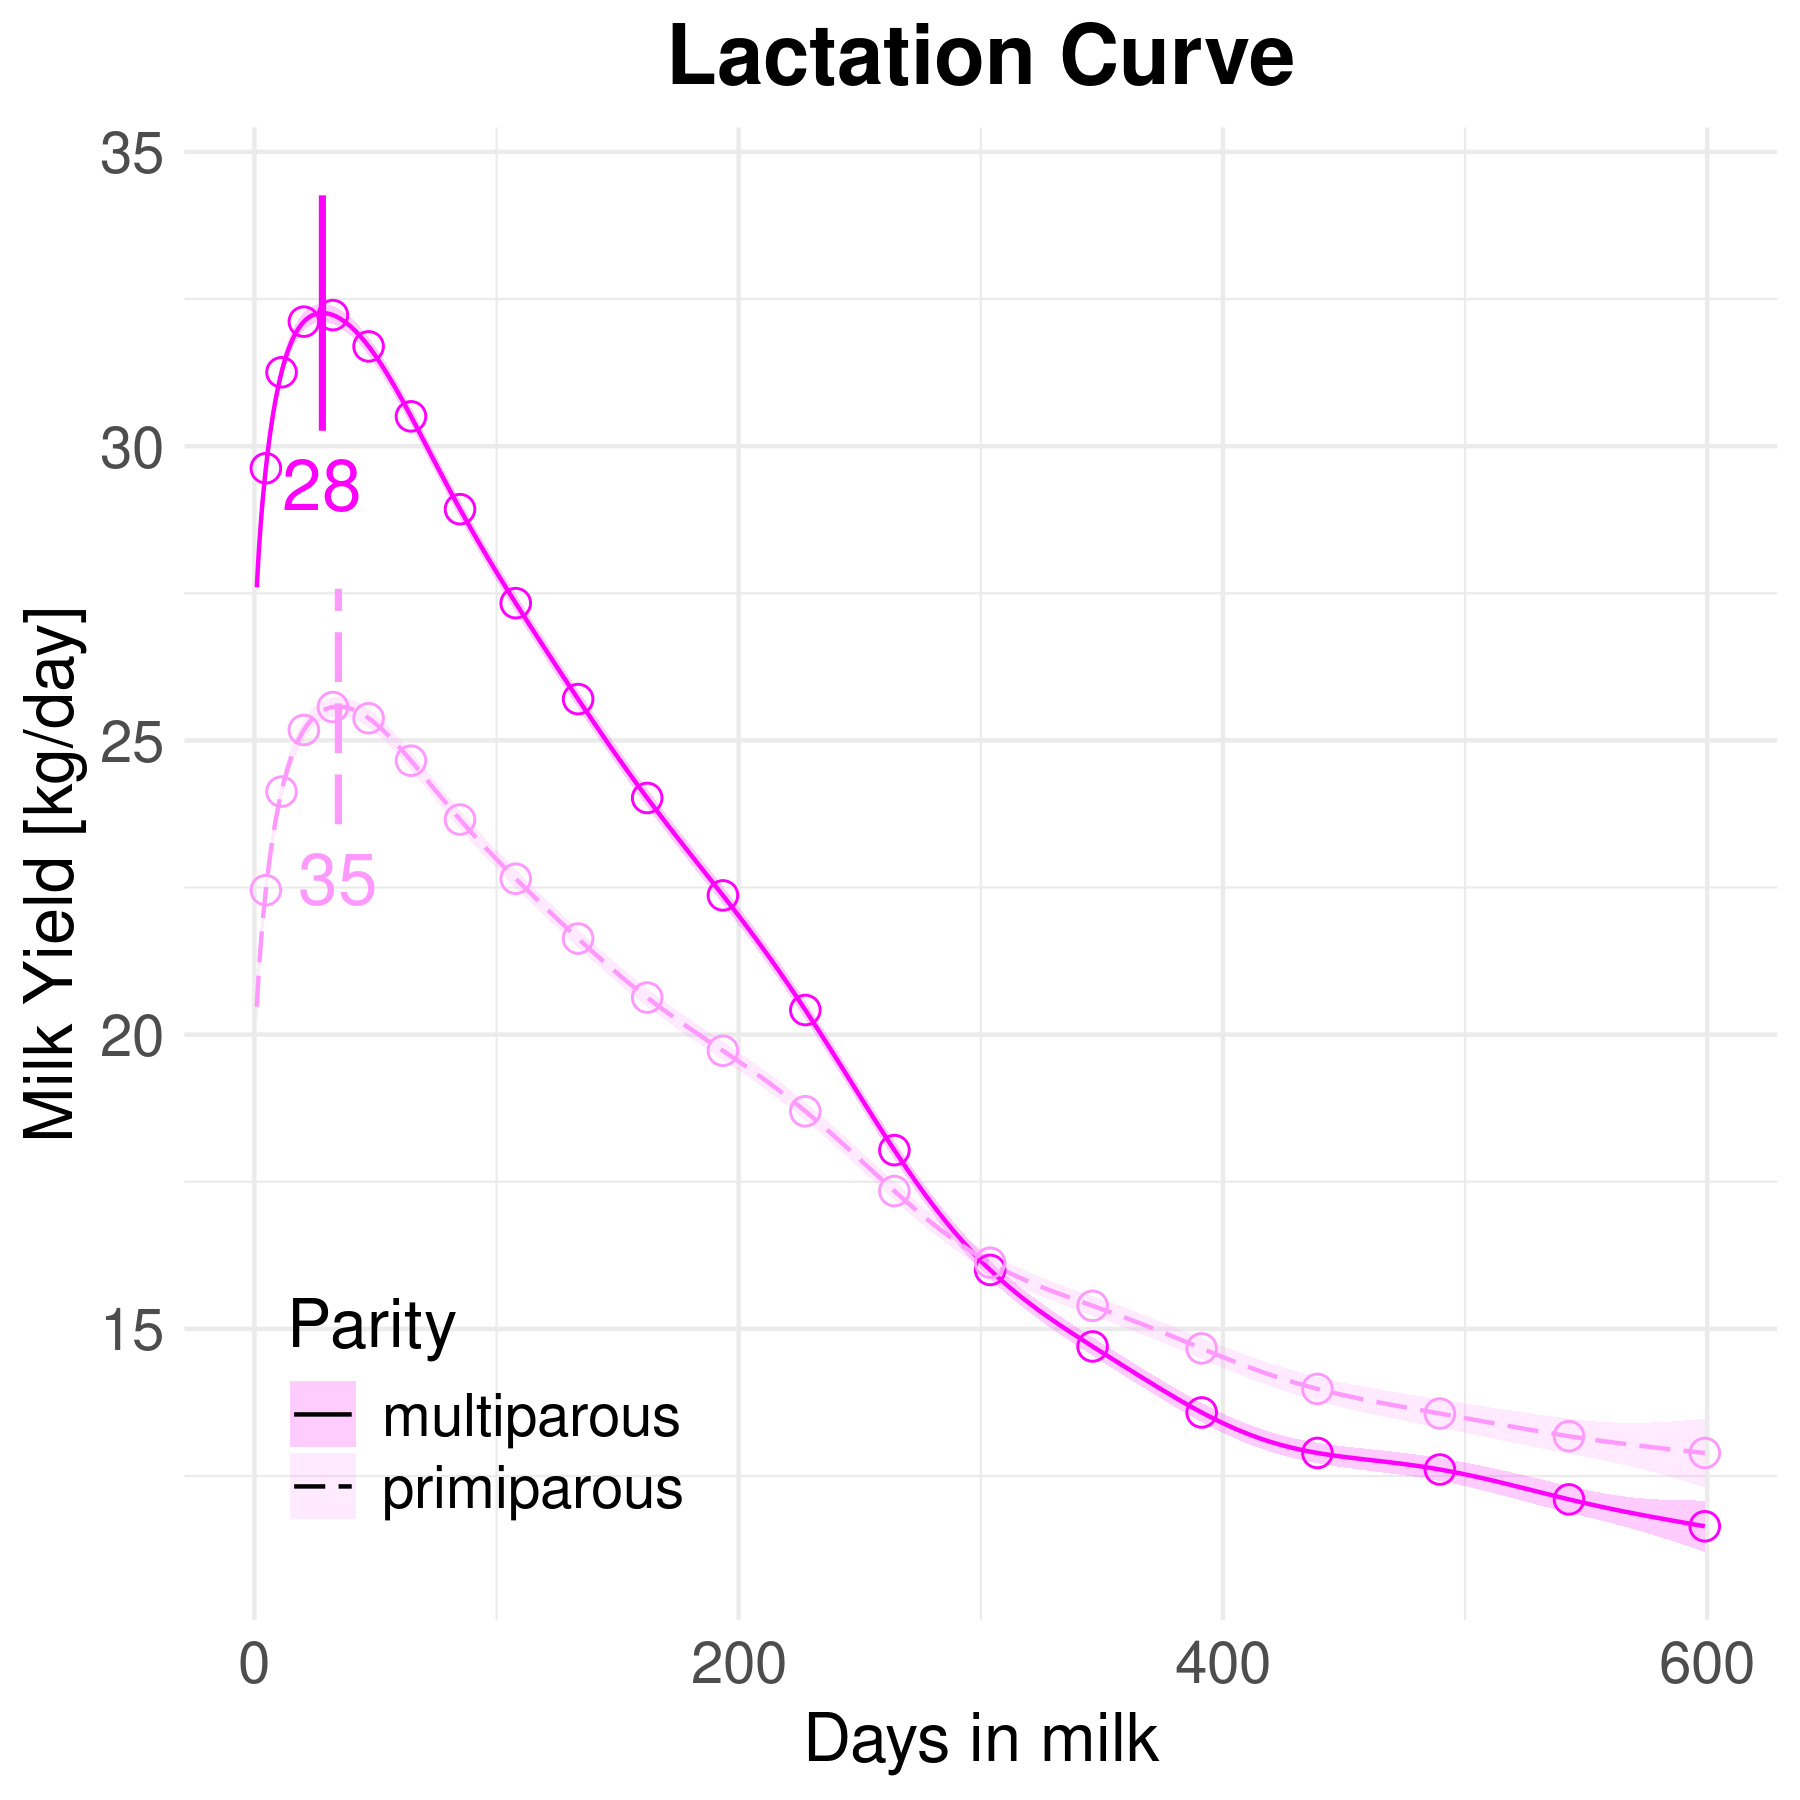
\includegraphics[width=\textwidth]{thesis/figures/models/milk/after2010/sf_milk_after2010/sf_milk_after2010_marginal_dim_milk_combined.png}
    \end{subfigure}
    \begin{subfigure}[b]{0.45\textwidth}
        \centering
        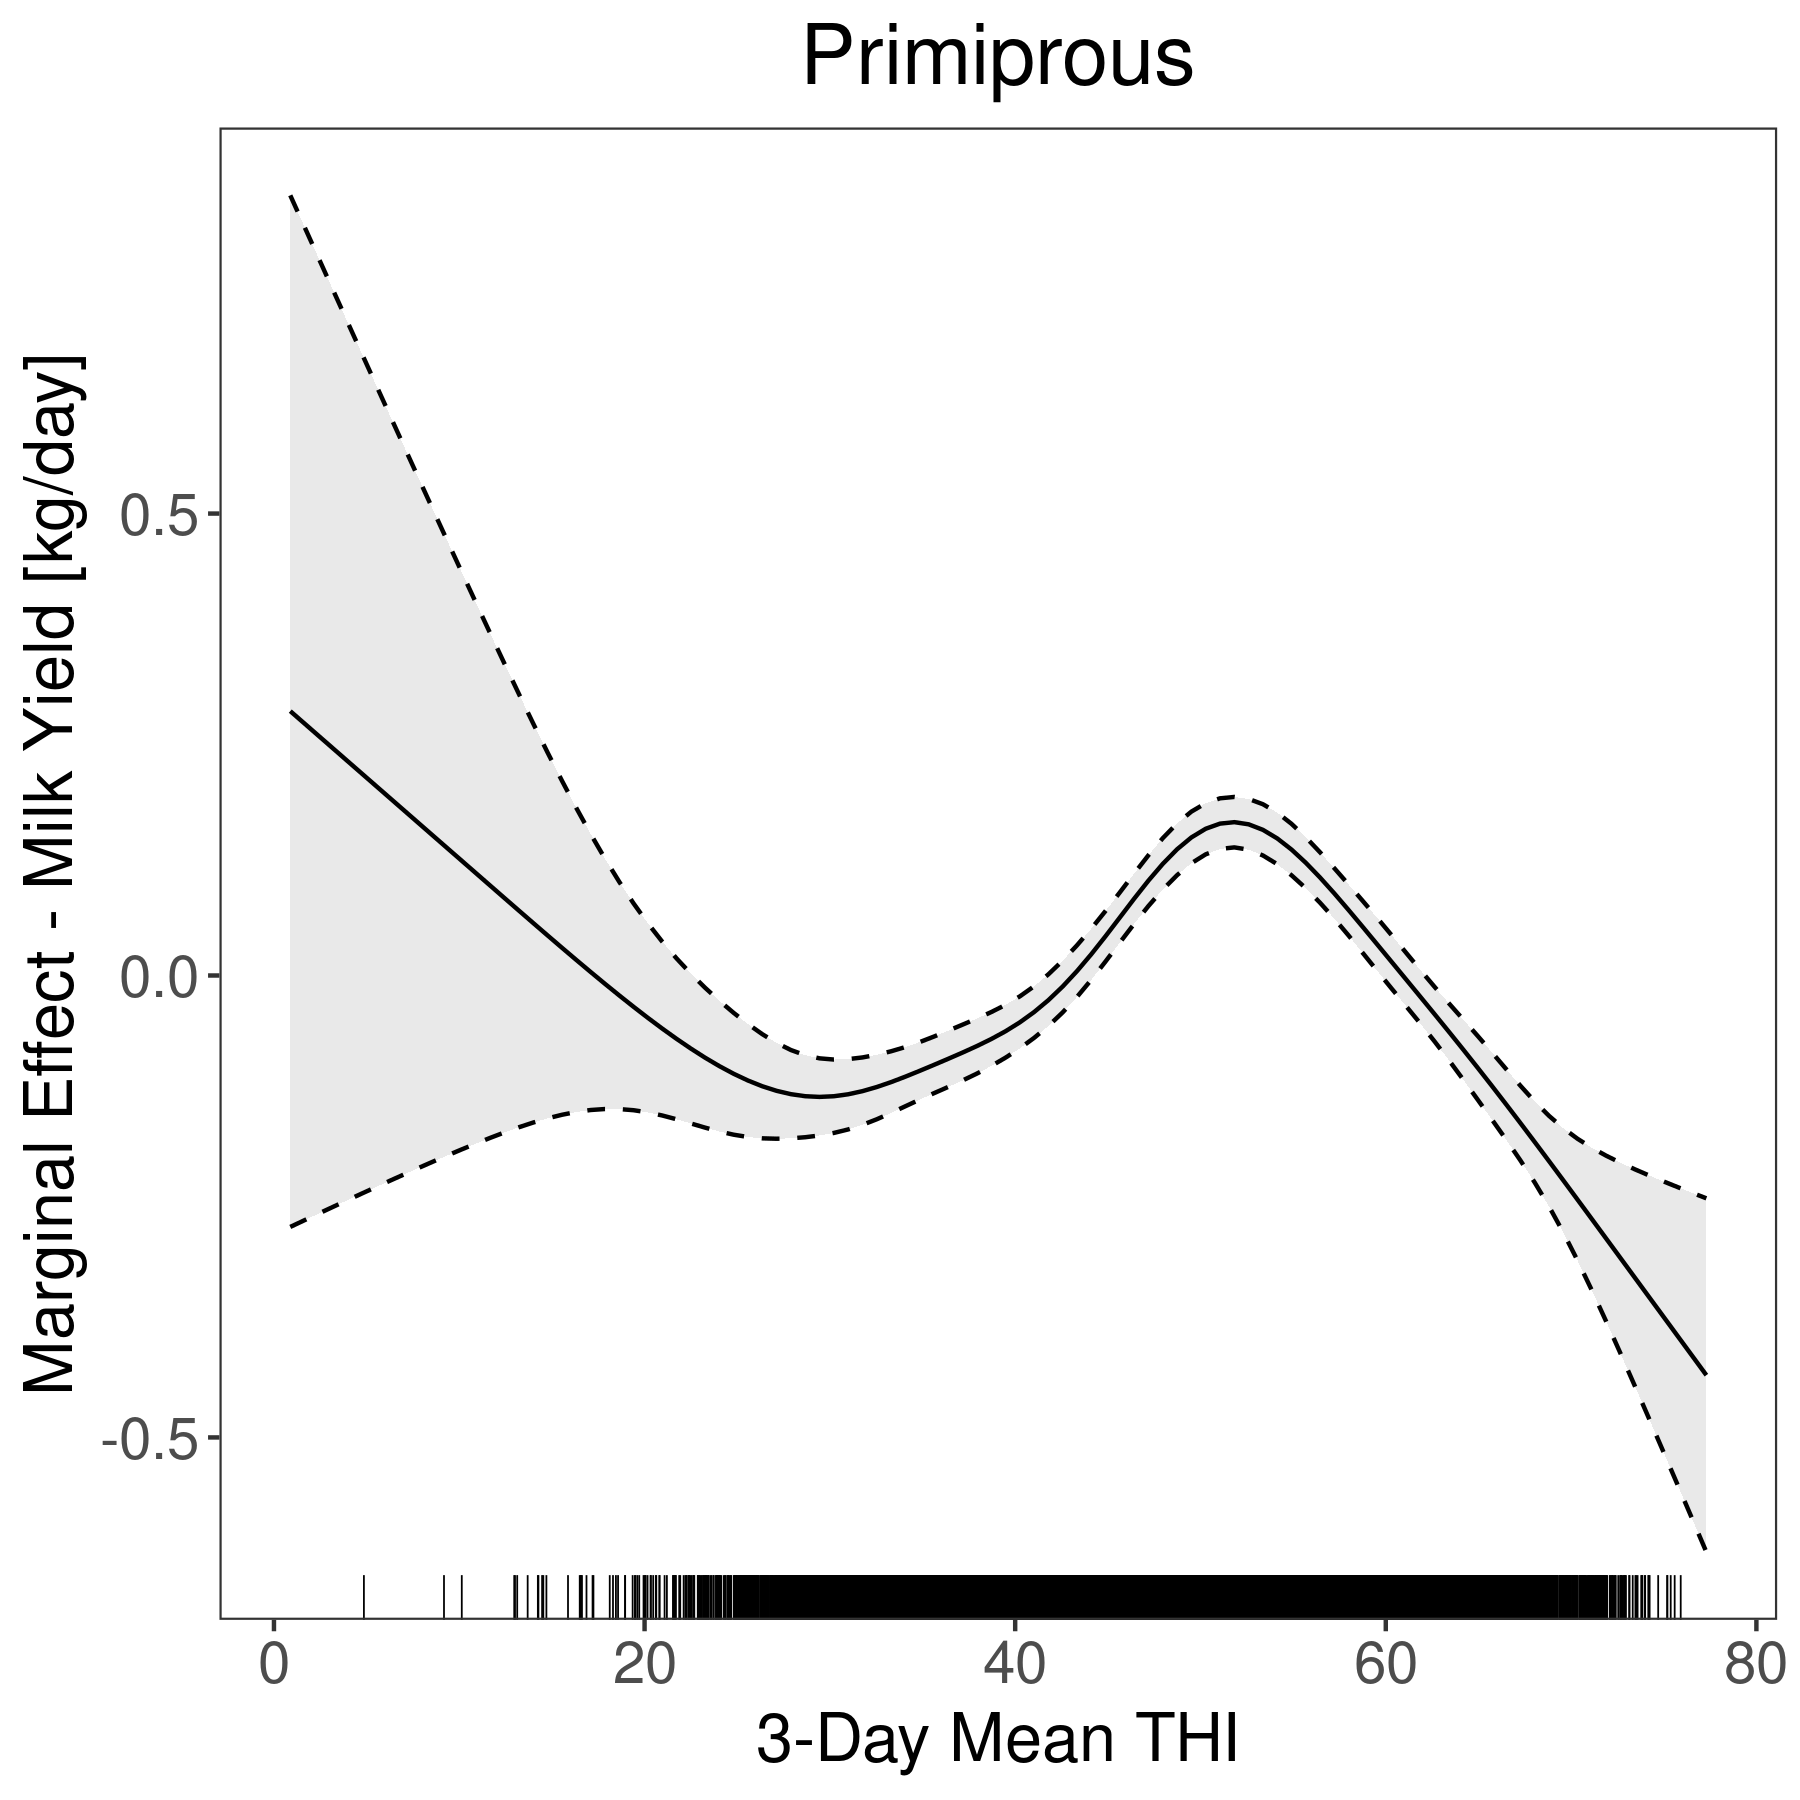
\includegraphics[width=\textwidth]{thesis/figures/models/milk/after2010/sf_milk_after2010/sf_milk_after2010_marginal_thi_milk_primi.png}
    \end{subfigure}
    \hspace{0.05\textwidth} % Optional space between the figures
    \begin{subfigure}[b]{0.45\textwidth}
        \centering
        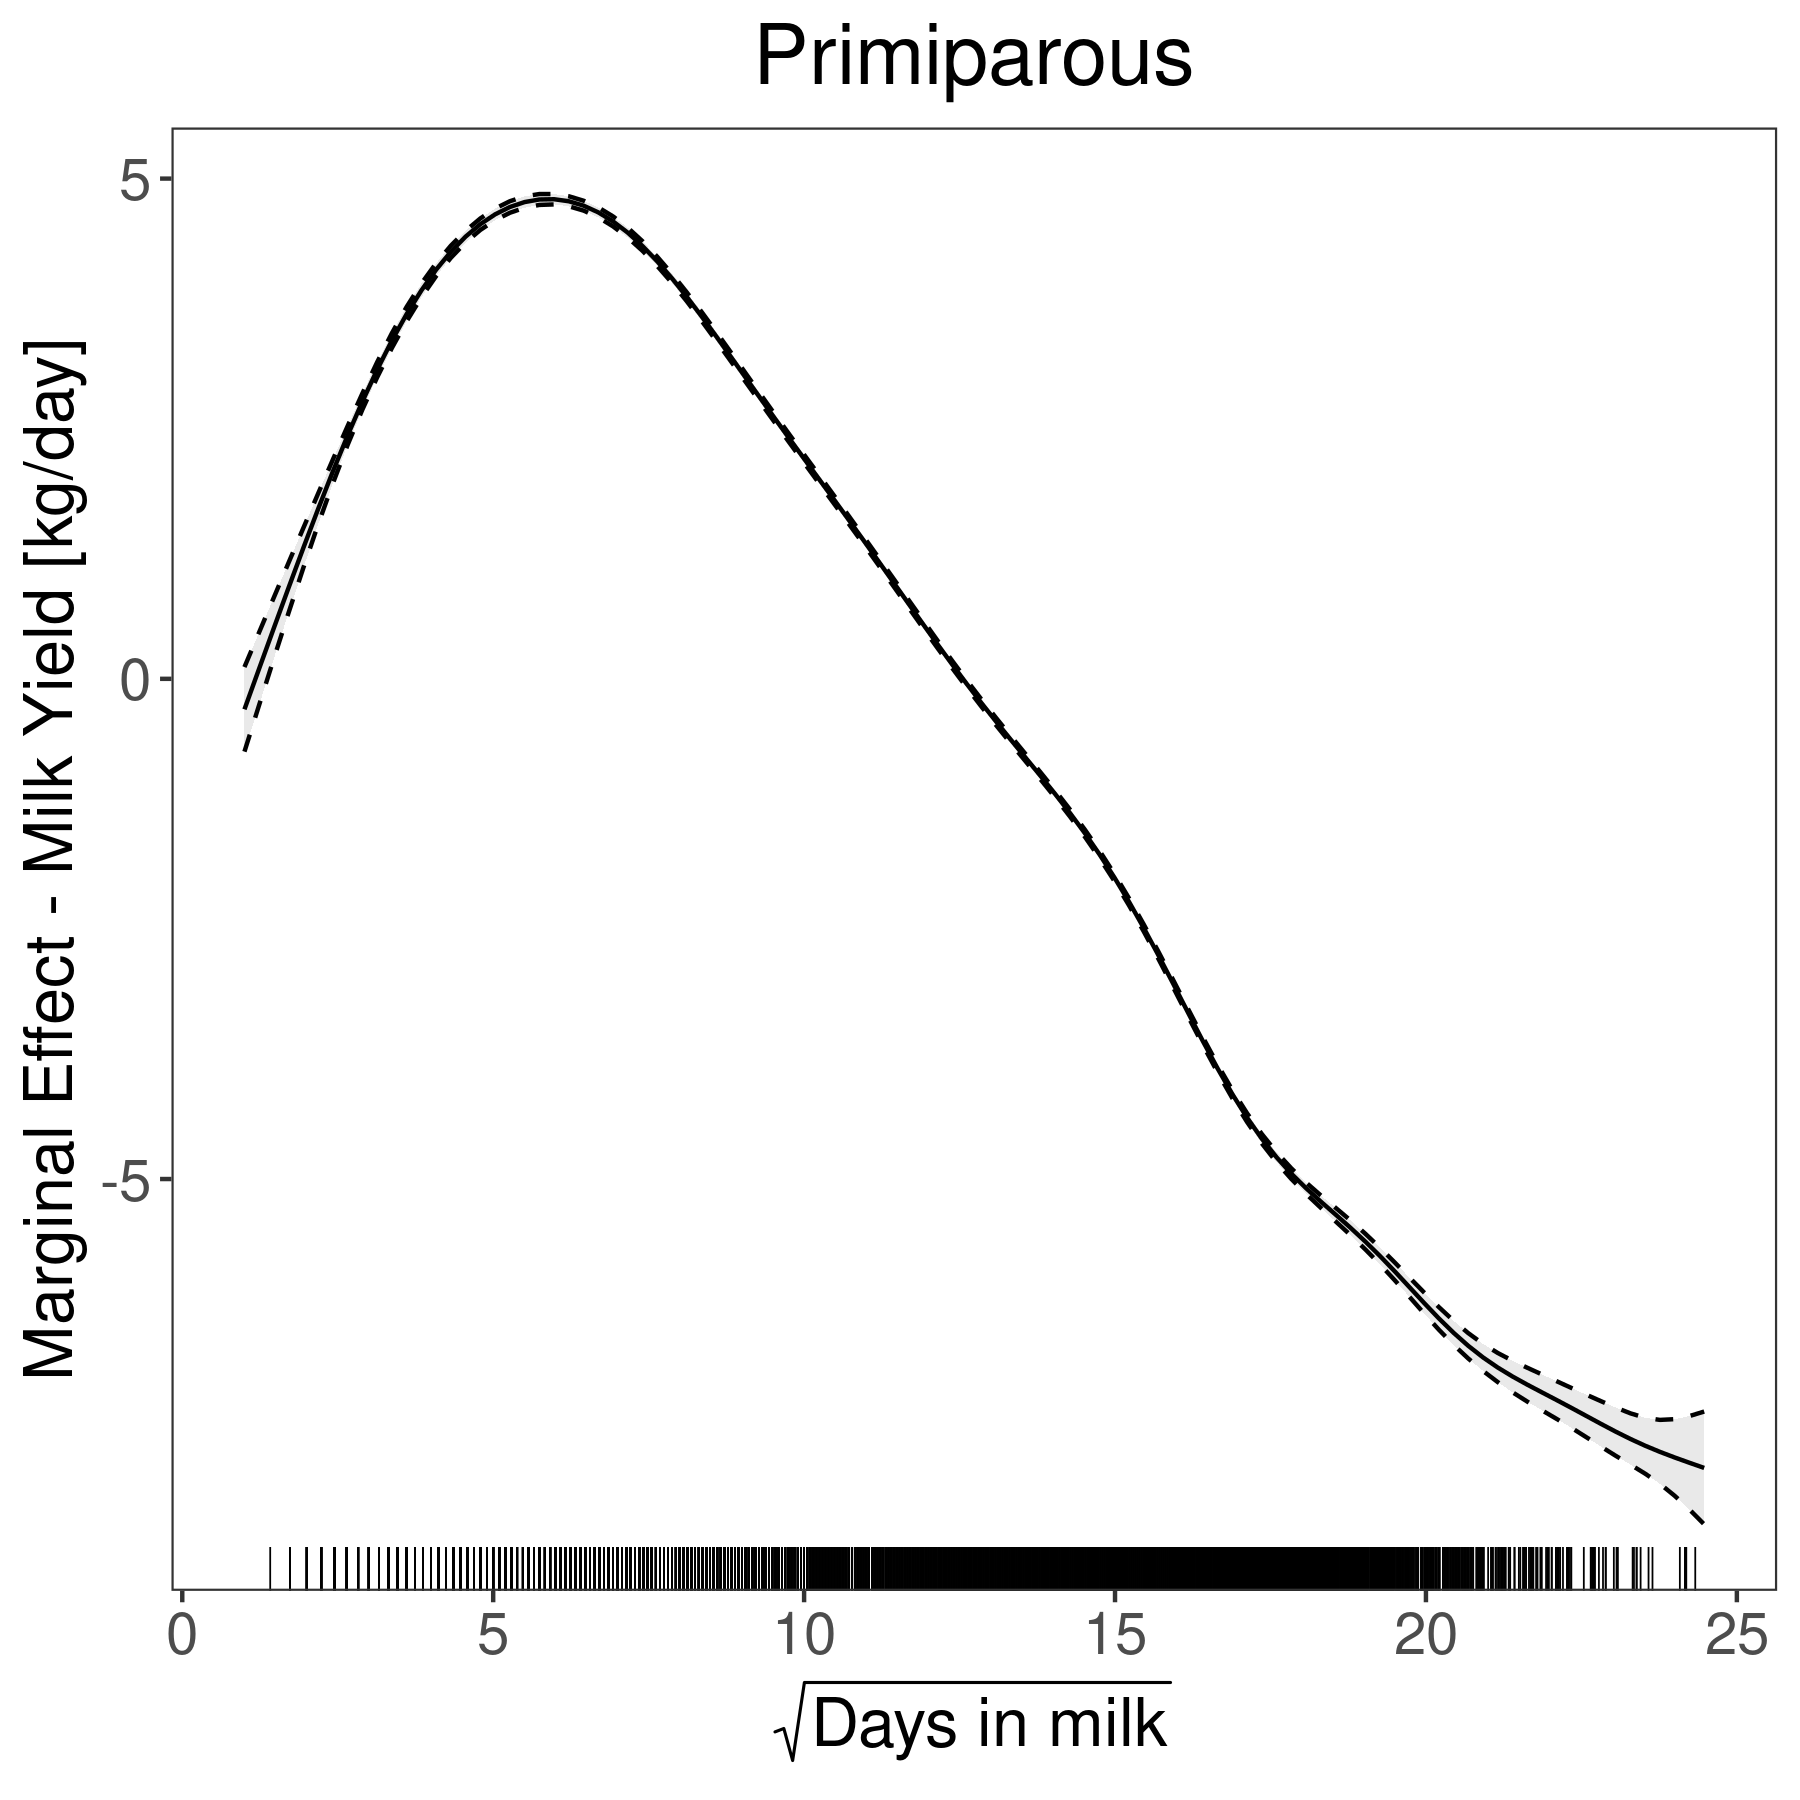
\includegraphics[width=\textwidth]{thesis/figures/models/milk/after2010/sf_milk_after2010/sf_milk_after2010_marginal_dim_milk_primi.png}
    \end{subfigure}
    \begin{subfigure}[b]{0.45\textwidth}
        \centering
        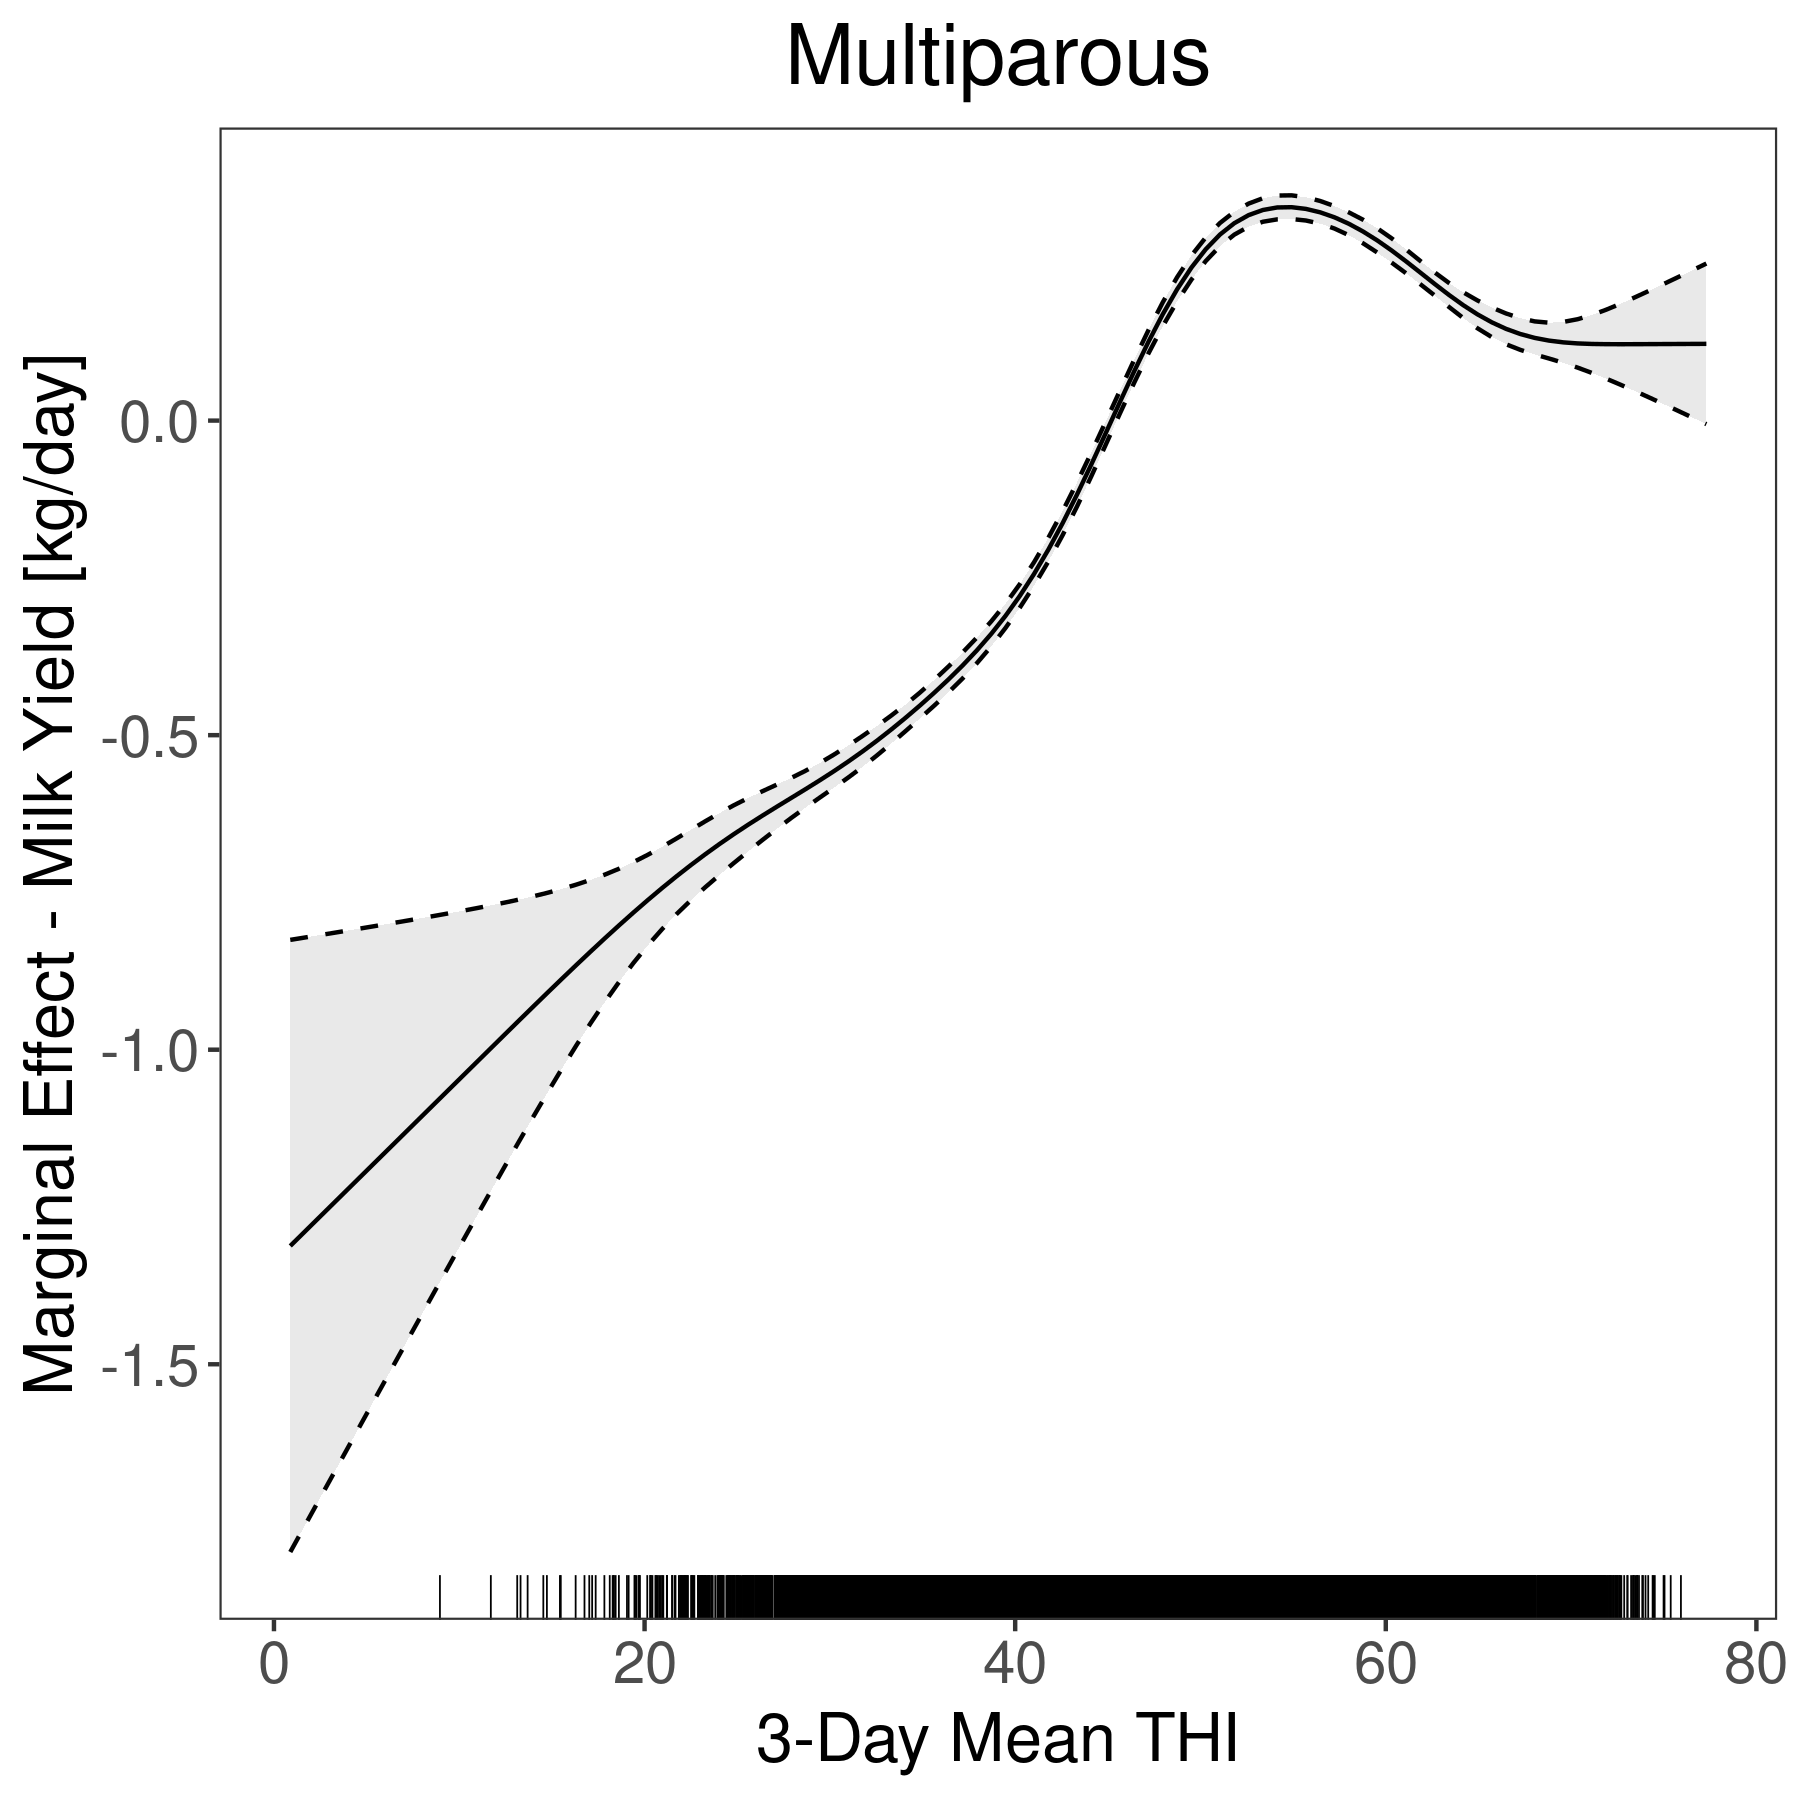
\includegraphics[width=\textwidth]{thesis/figures/models/milk/after2010/sf_milk_after2010/sf_milk_after2010_marginal_thi_milk_multi.png}
    \end{subfigure}
    \hspace{0.05\textwidth} % Optional space between the figures
    \begin{subfigure}[b]{0.45\textwidth}
        \centering
        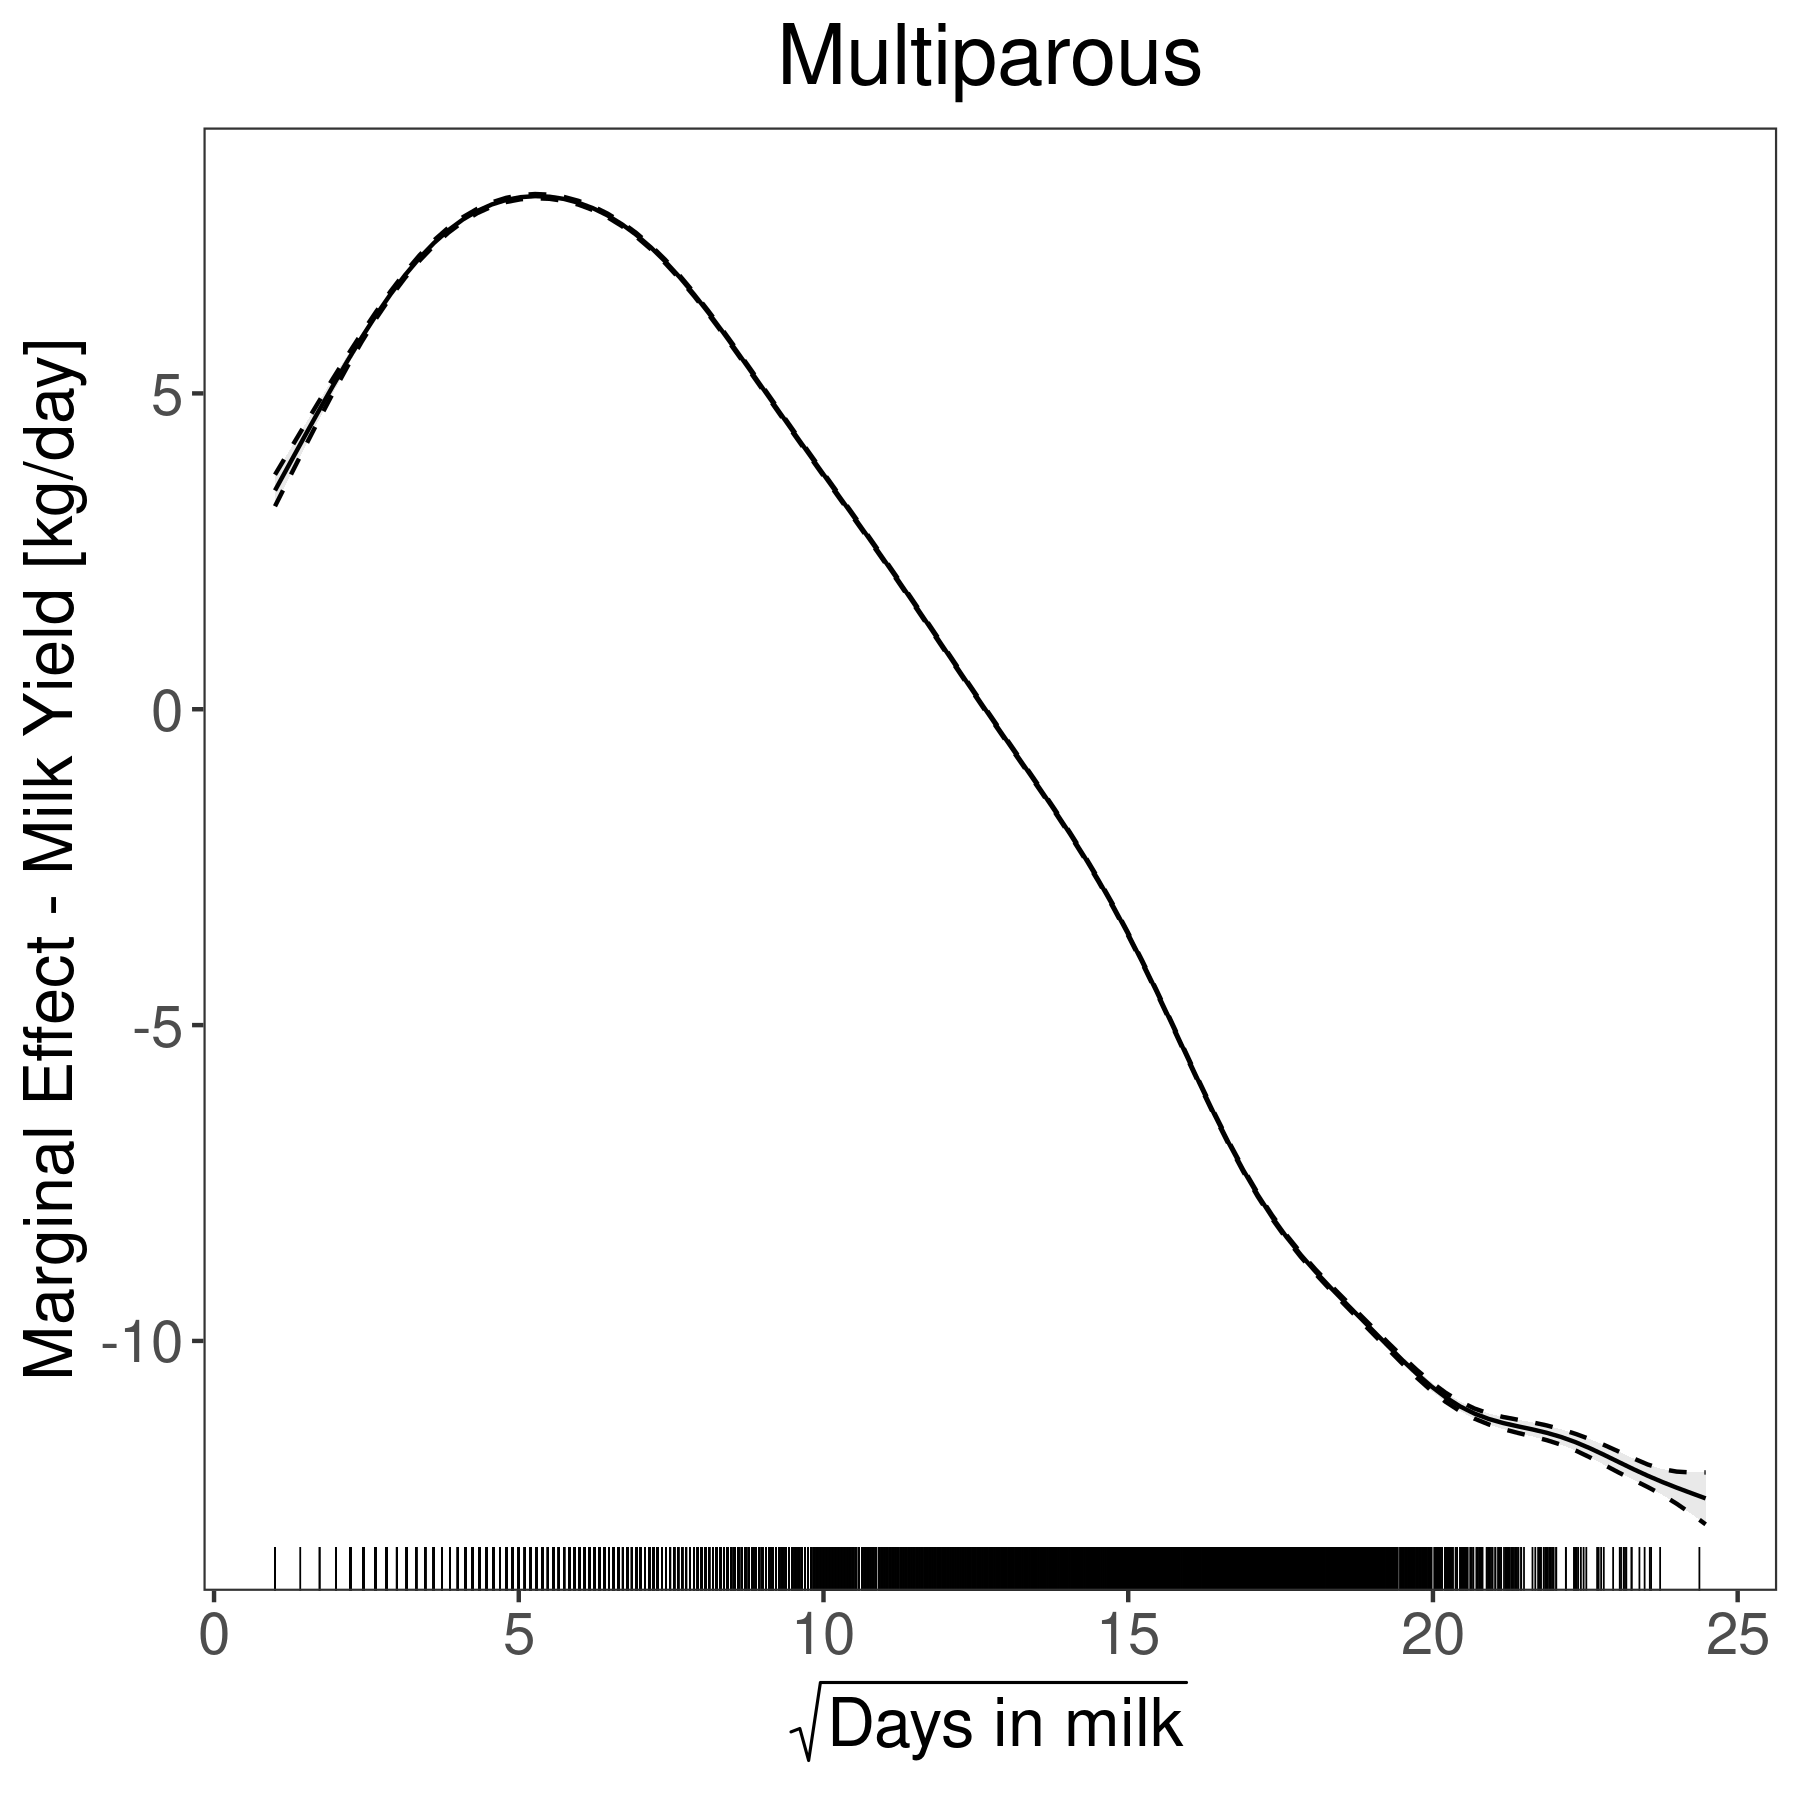
\includegraphics[width=\textwidth]{thesis/figures/models/milk/after2010/sf_milk_after2010/sf_milk_after2010_marginal_dim_milk_multi.png}
    \end{subfigure}
    \caption[]{Swiss Fleckvieh: Milk Yield - 2011 - 2023 - THI Effect and Lactation Curve}
    \label{fig:main}
\end{figure}
\addtocontents{toc}{\protect\setcounter{tocdepth}{2}}

\section{Swiss Fleckvieh: ECM Yield}
\subsection{Full Period: 1984-2023}\label{model:sf_ecm_full}
\paragraph{Model Summary} \quad \\

    \begin{table}[H]
    \centering
    \begin{tabular}{lrrrr}
    \textbf{A. parametric coefficients} & Estimate & Std. Error & t-value & p-value \\ 
       \hline
       \hline
      (Intercept) & 18.9428 & 2.0368 & 9.3002 & $<$ 0.0001 \\ 
      parityprimiparous & -3.3689 & 0.0142 & -236.8632 & $<$ 0.0001 \\ 
      year1985 & 0.4371 & 2.0474 & 0.2135 & 0.8309 \\ 
      year1986 & 0.3102 & 2.0464 & 0.1516 & 0.8795 \\ 
      year1987 & 0.0716 & 2.0478 & 0.0349 & 0.9721 \\ 
      year1988 & -0.3584 & 2.0554 & -0.1744 & 0.8616 \\ 
      year1989 & 0.4960 & 2.0565 & 0.2412 & 0.8094 \\ 
      year1990 & 0.9176 & 2.0553 & 0.4464 & 0.6553 \\ 
      year1991 & 1.1455 & 2.0556 & 0.5572 & 0.5774 \\ 
      year1992 & 1.4593 & 2.0517 & 0.7113 & 0.4769 \\ 
      year1993 & 1.3829 & 2.0517 & 0.6740 & 0.5003 \\ 
      year1994 & 1.2177 & 2.0522 & 0.5933 & 0.5530 \\ 
      year1995 & 1.5433 & 2.0564 & 0.7505 & 0.4530 \\ 
      year1996 & 1.7761 & 2.0557 & 0.8640 & 0.3876 \\ 
      year1997 & 2.2786 & 2.0564 & 1.1081 & 0.2678 \\ 
      year1998 & 3.1880 & 2.0566 & 1.5502 & 0.1211 \\ 
      year1999 & 3.1331 & 2.0596 & 1.5212 & 0.1282 \\ 
      year2000 & 3.0081 & 2.0612 & 1.4594 & 0.1445 \\ 
      year2001 & 3.3840 & 2.0762 & 1.6299 & 0.1031 \\ 
      year2002 & 3.4445 & 2.0684 & 1.6653 & 0.0959 \\ 
      year2003 & 3.9752 & 2.0675 & 1.9227 & 0.0545 \\ 
      year2004 & 4.4635 & 2.0679 & 2.1585 & 0.0309 \\ 
      year2005 & 4.8537 & 2.0704 & 2.3444 & 0.0191 \\ 
      year2006 & 4.7686 & 2.0692 & 2.3046 & 0.0212 \\ 
      year2007 & 4.4191 & 2.0694 & 2.1354 & 0.0327 \\ 
      year2008 & 4.6589 & 2.0682 & 2.2526 & 0.0243 \\ 
      year2009 & 4.8424 & 2.0665 & 2.3433 & 0.0191 \\ 
      year2010 & 5.3358 & 2.0644 & 2.5847 & 0.0097 \\ 
      year2011 & 5.2852 & 2.0614 & 2.5639 & 0.0104 \\ 
      year2012 & 5.2468 & 2.0608 & 2.5460 & 0.0109 \\ 
      year2013 & 5.0911 & 2.0603 & 2.4711 & 0.0135 \\ 
      year2014 & 5.6526 & 2.0607 & 2.7430 & 0.0061 \\ 
      year2015 & 6.1039 & 2.0609 & 2.9618 & 0.0031 \\ 
      year2016 & 6.3861 & 2.0608 & 3.0989 & 0.0019 \\ 
      year2017 & 6.4411 & 2.0613 & 3.1249 & 0.0018 \\ 
      year2018 & 7.2593 & 2.0617 & 3.5210 & 0.0004 \\ 
      year2019 & 7.3393 & 2.0627 & 3.5581 & 0.0004 \\ 
      year2020 & 7.8516 & 2.0673 & 3.7979 & 0.0001 \\ 
      year2021 & 8.0252 & 2.0703 & 3.8763 & 0.0001 \\ 
      year2022 & 7.7722 & 2.0760 & 3.7437 & 0.0002 \\ 
      year2023 & 8.3910 & 2.0798 & 4.0346 & 0.0001 \\ 
       \hline
    \textbf{B. smooth terms} & edf & Ref.df & F-value & p-value \\ 
    \hline
    \hline
      s(thi\_mean\_t0\_3d):paritymultiparous & 8.5041 & 8.5041 & 234.1182 & $<$ 0.0001 \\ 
      s(thi\_mean\_t0\_3d):parityprimiparous & 6.4177 & 6.4177 & 140.2851 & $<$ 0.0001 \\ 
      s(days\_in\_milk\_t):paritymultiparous & 14.1442 & 14.1442 & 103387.1413 & $<$ 0.0001 \\ 
      s(days\_in\_milk\_t):parityprimiparous & 12.3534 & 12.3534 & 9446.9365 & $<$ 0.0001 \\ 
       \hline
    \end{tabular}
    \caption[]{Swiss Fleckvieh: ECM Yield - 1984-2023 - GAMM model summary without random effect terms.}
    \end{table}

\newpage
\begin{table}[H]
\centering
\begin{tabular}
{l | r | r | r | r}
\textbf{Smooth Term Fixed Effect} & Est. & SE & z & p\\
\hline
\hline
s(thi\_mean\_t0\_3d):multiFx1 & 0.4379 & 0.0980 & 4.47 & $<$ 1e-05\\
s(thi\_mean\_t0\_3d):primiFx1 & 0.5091 & 0.1123 & 4.53 & $<$ 1e-05\\
s(days\_in\_milk\_):multiFx1 & 0.1549 & 0.5426 & 0.29 & 0.7752\\
s(days\_in\_milk\_):primiFx1 & -0.4183 & 0.5123 & -0.82 & 0.4142\\
\hline
\textbf{Variance Component} & Estimated $\sigma$ & & & \\
\hline
\hline
$\sigma_\alpha$ & 2.7441 & & & \\
$\sigma_\iota$ & 0.9269 & & & \\
$\sigma_\phi$ & 3.2102 & & & \\
s(thi\_mean\_t0\_3d):multi &  2.3885 & & & \\
s(days\_in\_milk\_):primi & 4.1628 & & & \\
s(days\_in\_milk\_):multi & 7.4804 & & & \\
s(thi\_mean\_t0\_3d):primi & 1.1828 & & & \\
Residual & 3.4443 & & & \\
\end{tabular}
\caption[]{Swiss Fleckvieh: ECM Yield - 1984-2023 - Mixed Model Summary - Smooth Terms and Random Effects.}
\end{table}


\paragraph{Model Diagnostics} \quad \\
\begin{figure}[H]
    \centering
    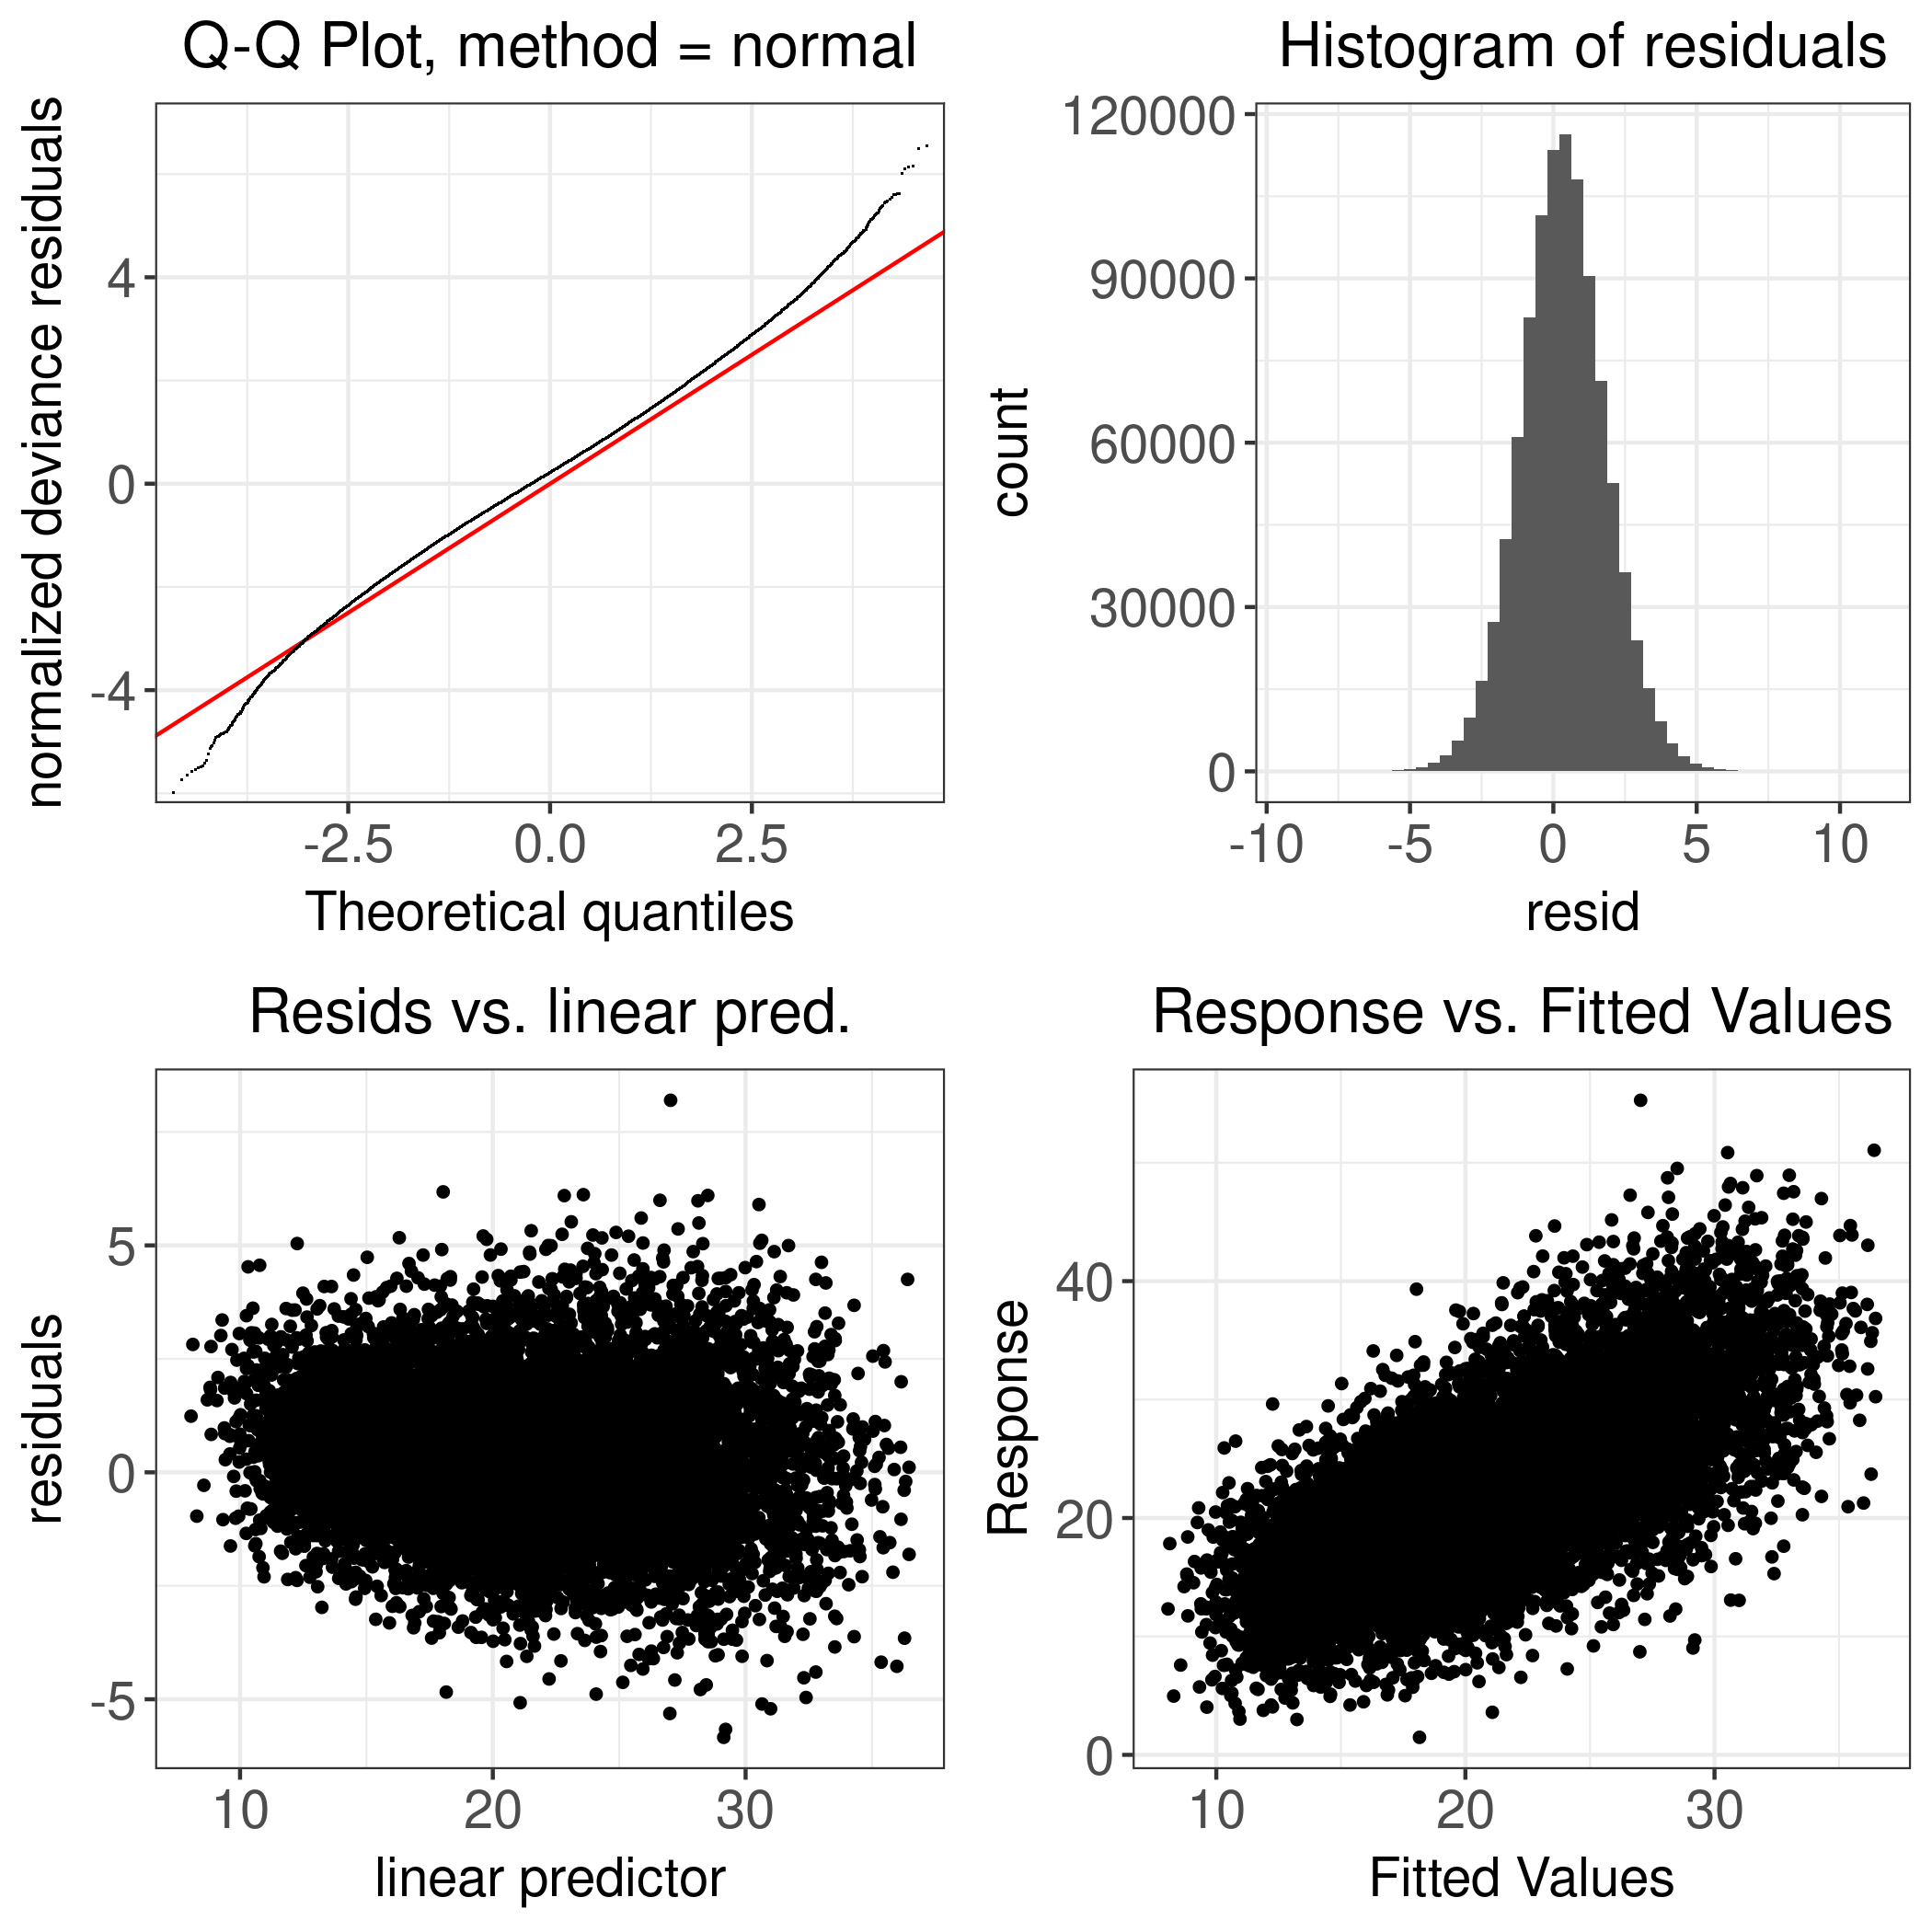
\includegraphics[width=0.6\textwidth]{thesis/figures/models/ecm/full/sf_ecm_full/sf_ecm_full_diagnostics.png}
    \caption[]{Swiss Fleckvieh: ECM Yield - 1984-2023 - Diagnostic Plot}
\end{figure}

\newpage
\paragraph{THI Effect and Lactation Curve} \quad \\
\begin{figure}[H]
    \centering
    \begin{subfigure}[b]{0.45\textwidth}
        \centering
        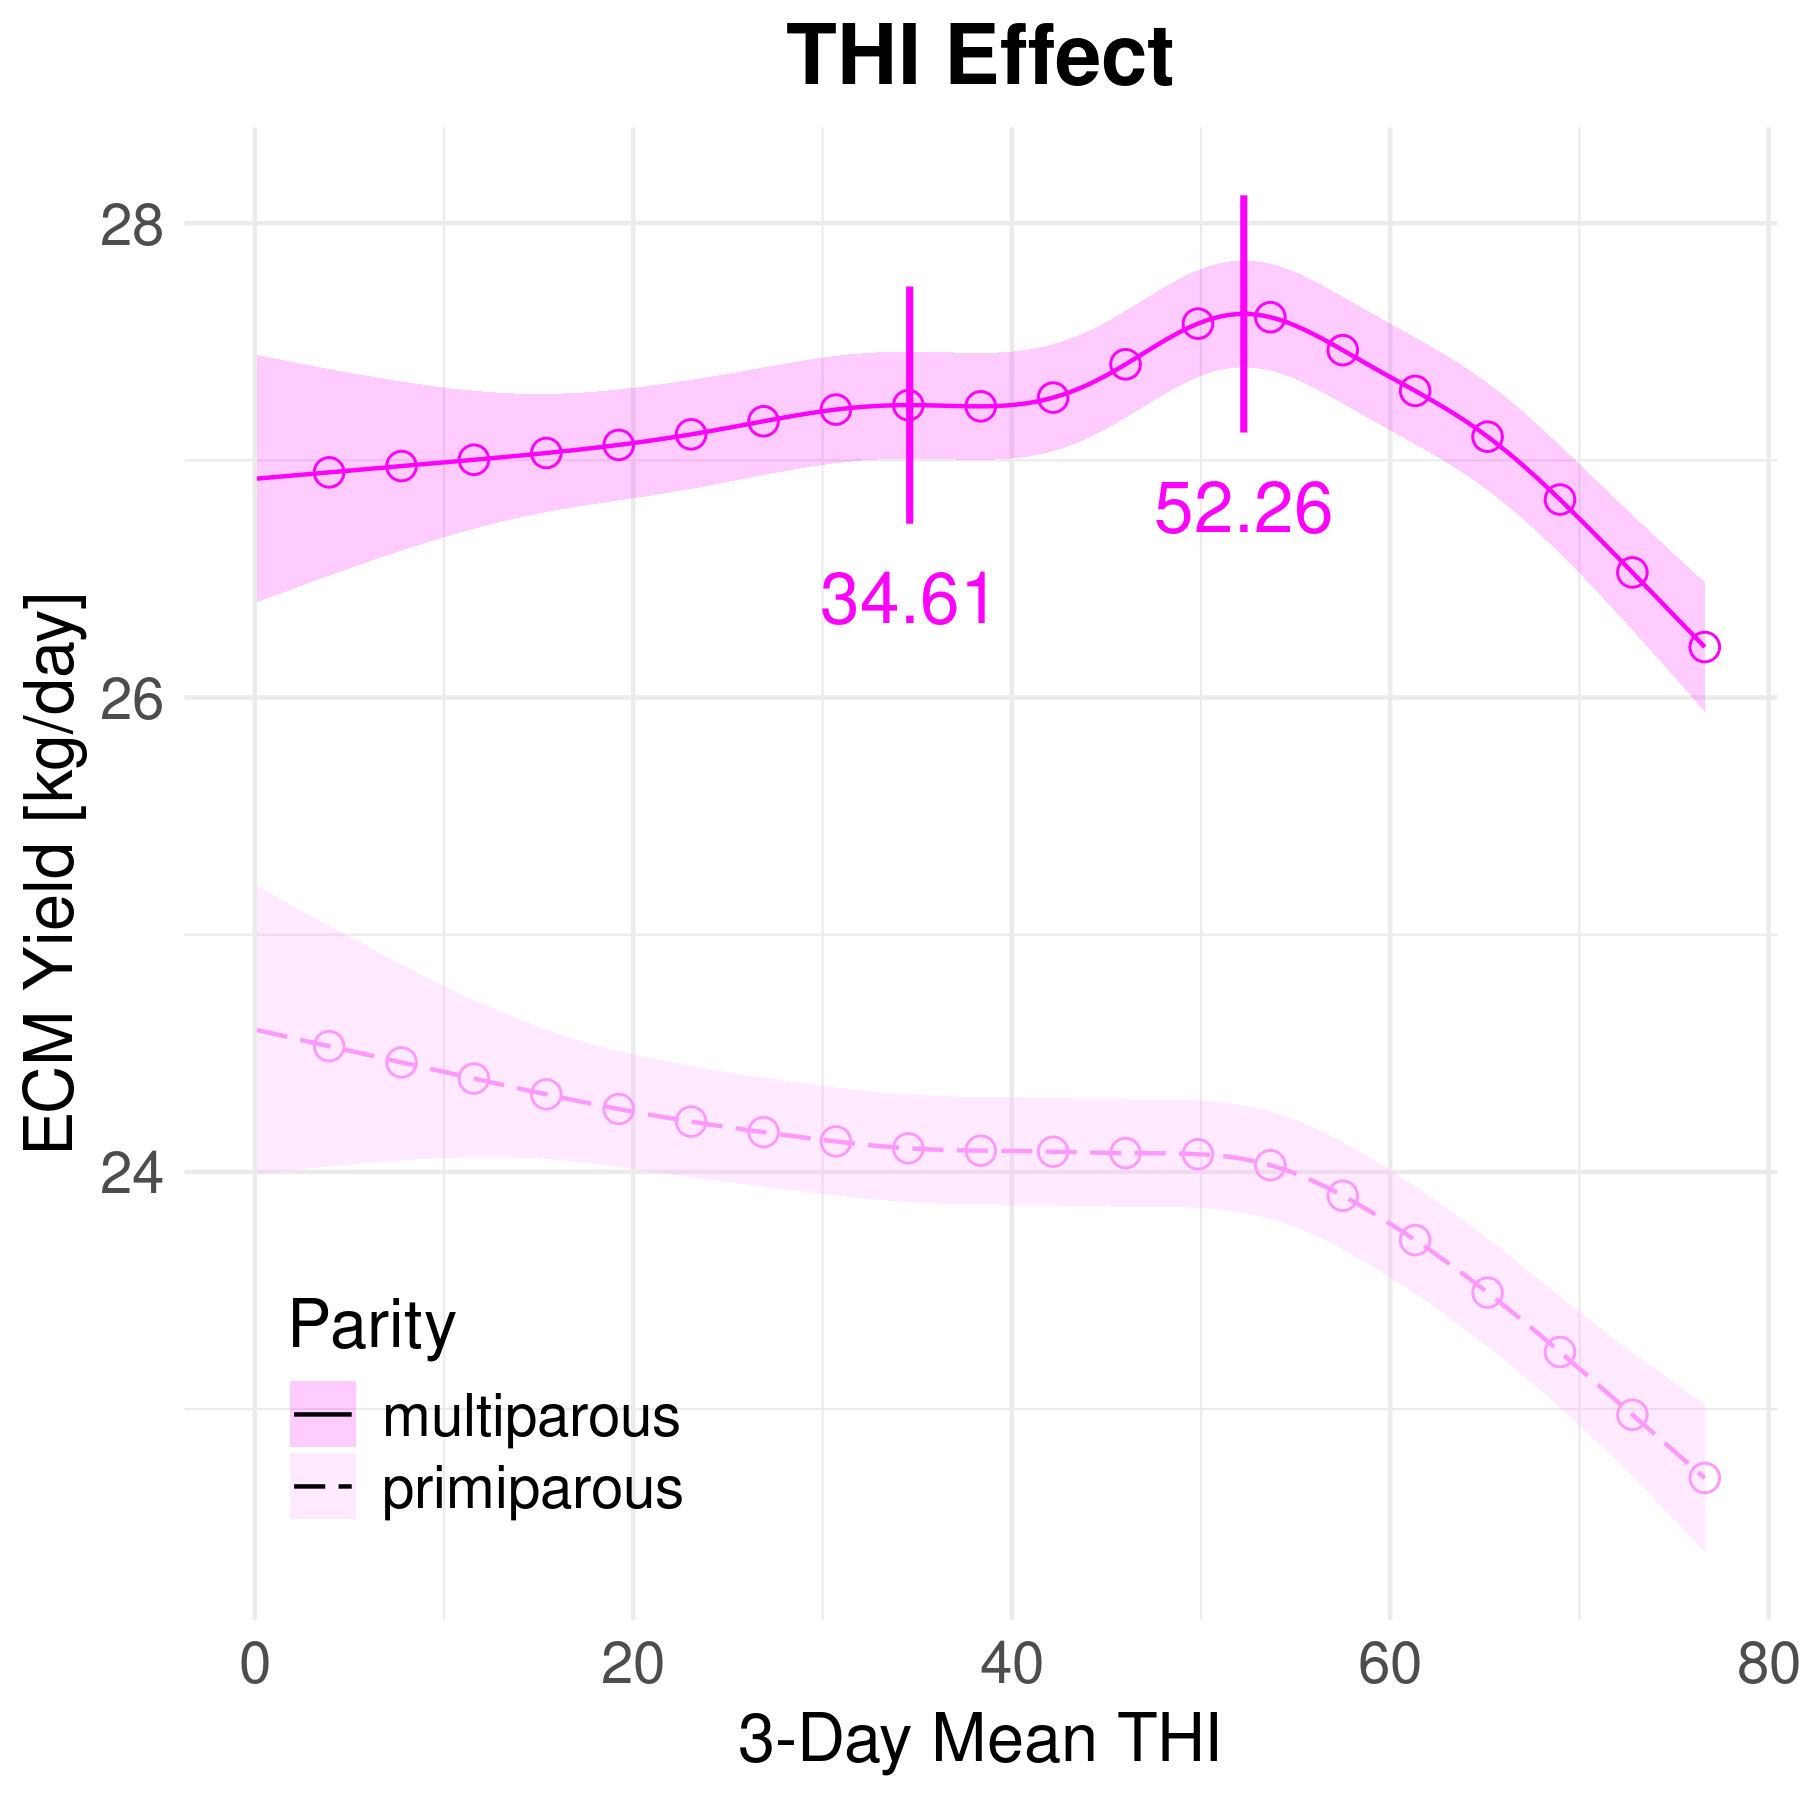
\includegraphics[width=\textwidth]{thesis/figures/models/ecm/full/sf_ecm_full/sf_ecm_full_marginal_thi_milk_combined.png}
    \end{subfigure}
    \hspace{0.05\textwidth} % Optional space between the figures
    \begin{subfigure}[b]{0.45\textwidth}
        \centering
        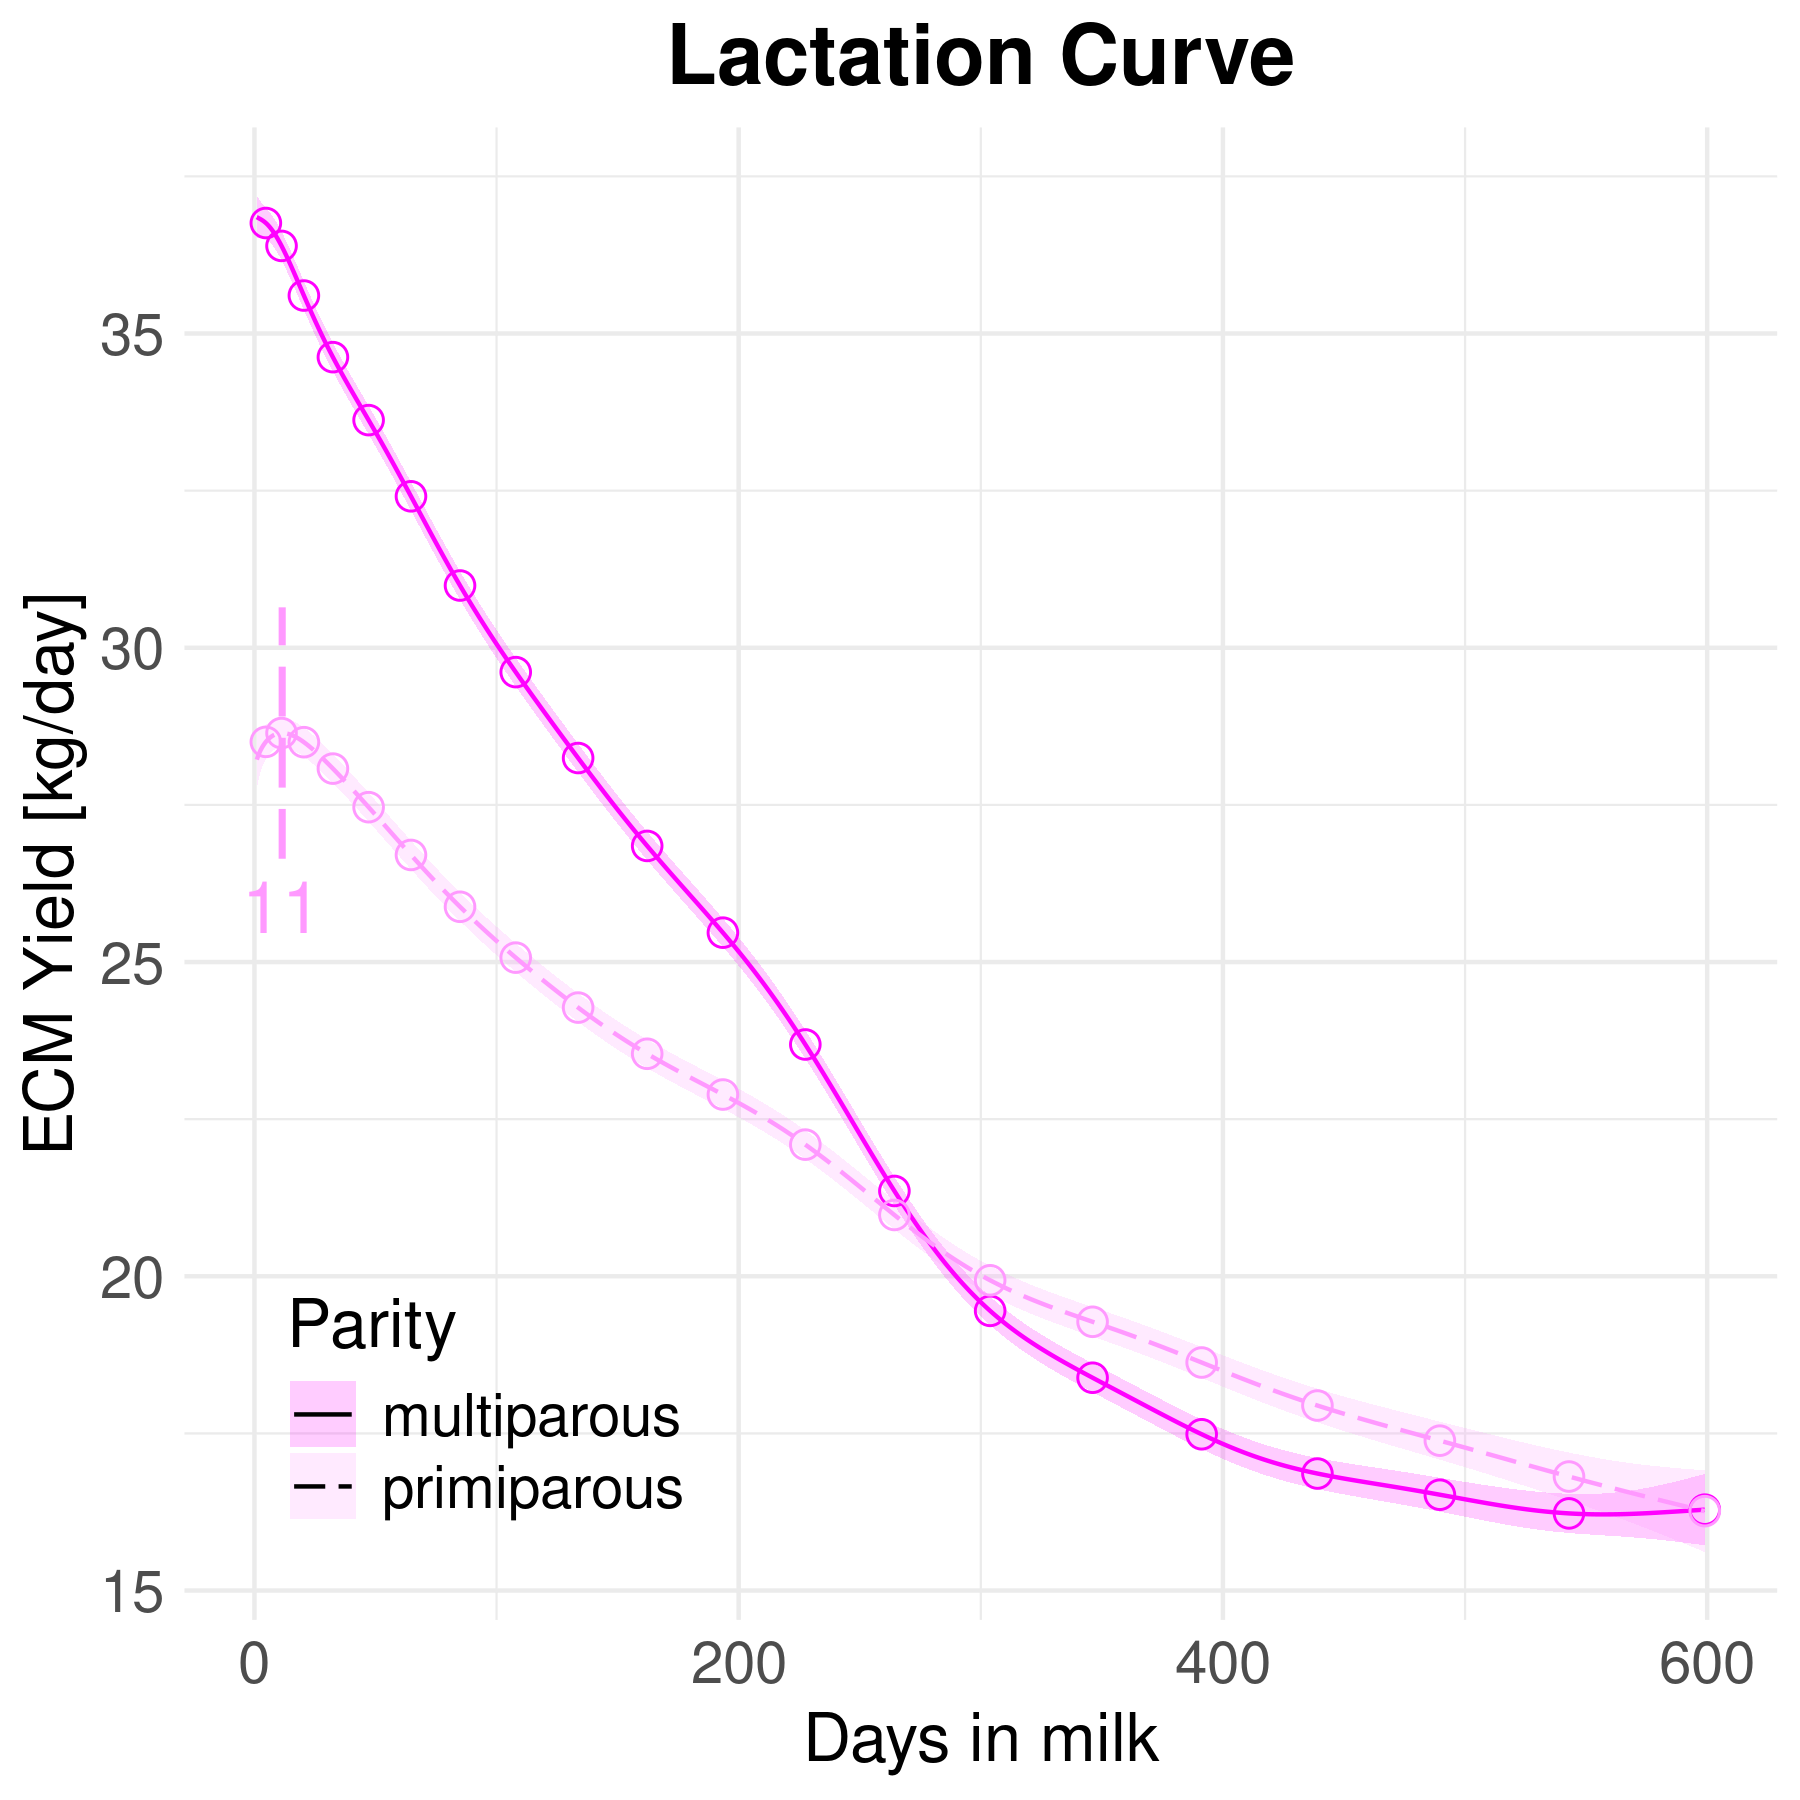
\includegraphics[width=\textwidth]{thesis/figures/models/ecm/full/sf_ecm_full/sf_ecm_full_marginal_dim_milk_combined.png}
    \end{subfigure}
    \begin{subfigure}[b]{0.45\textwidth}
        \centering
        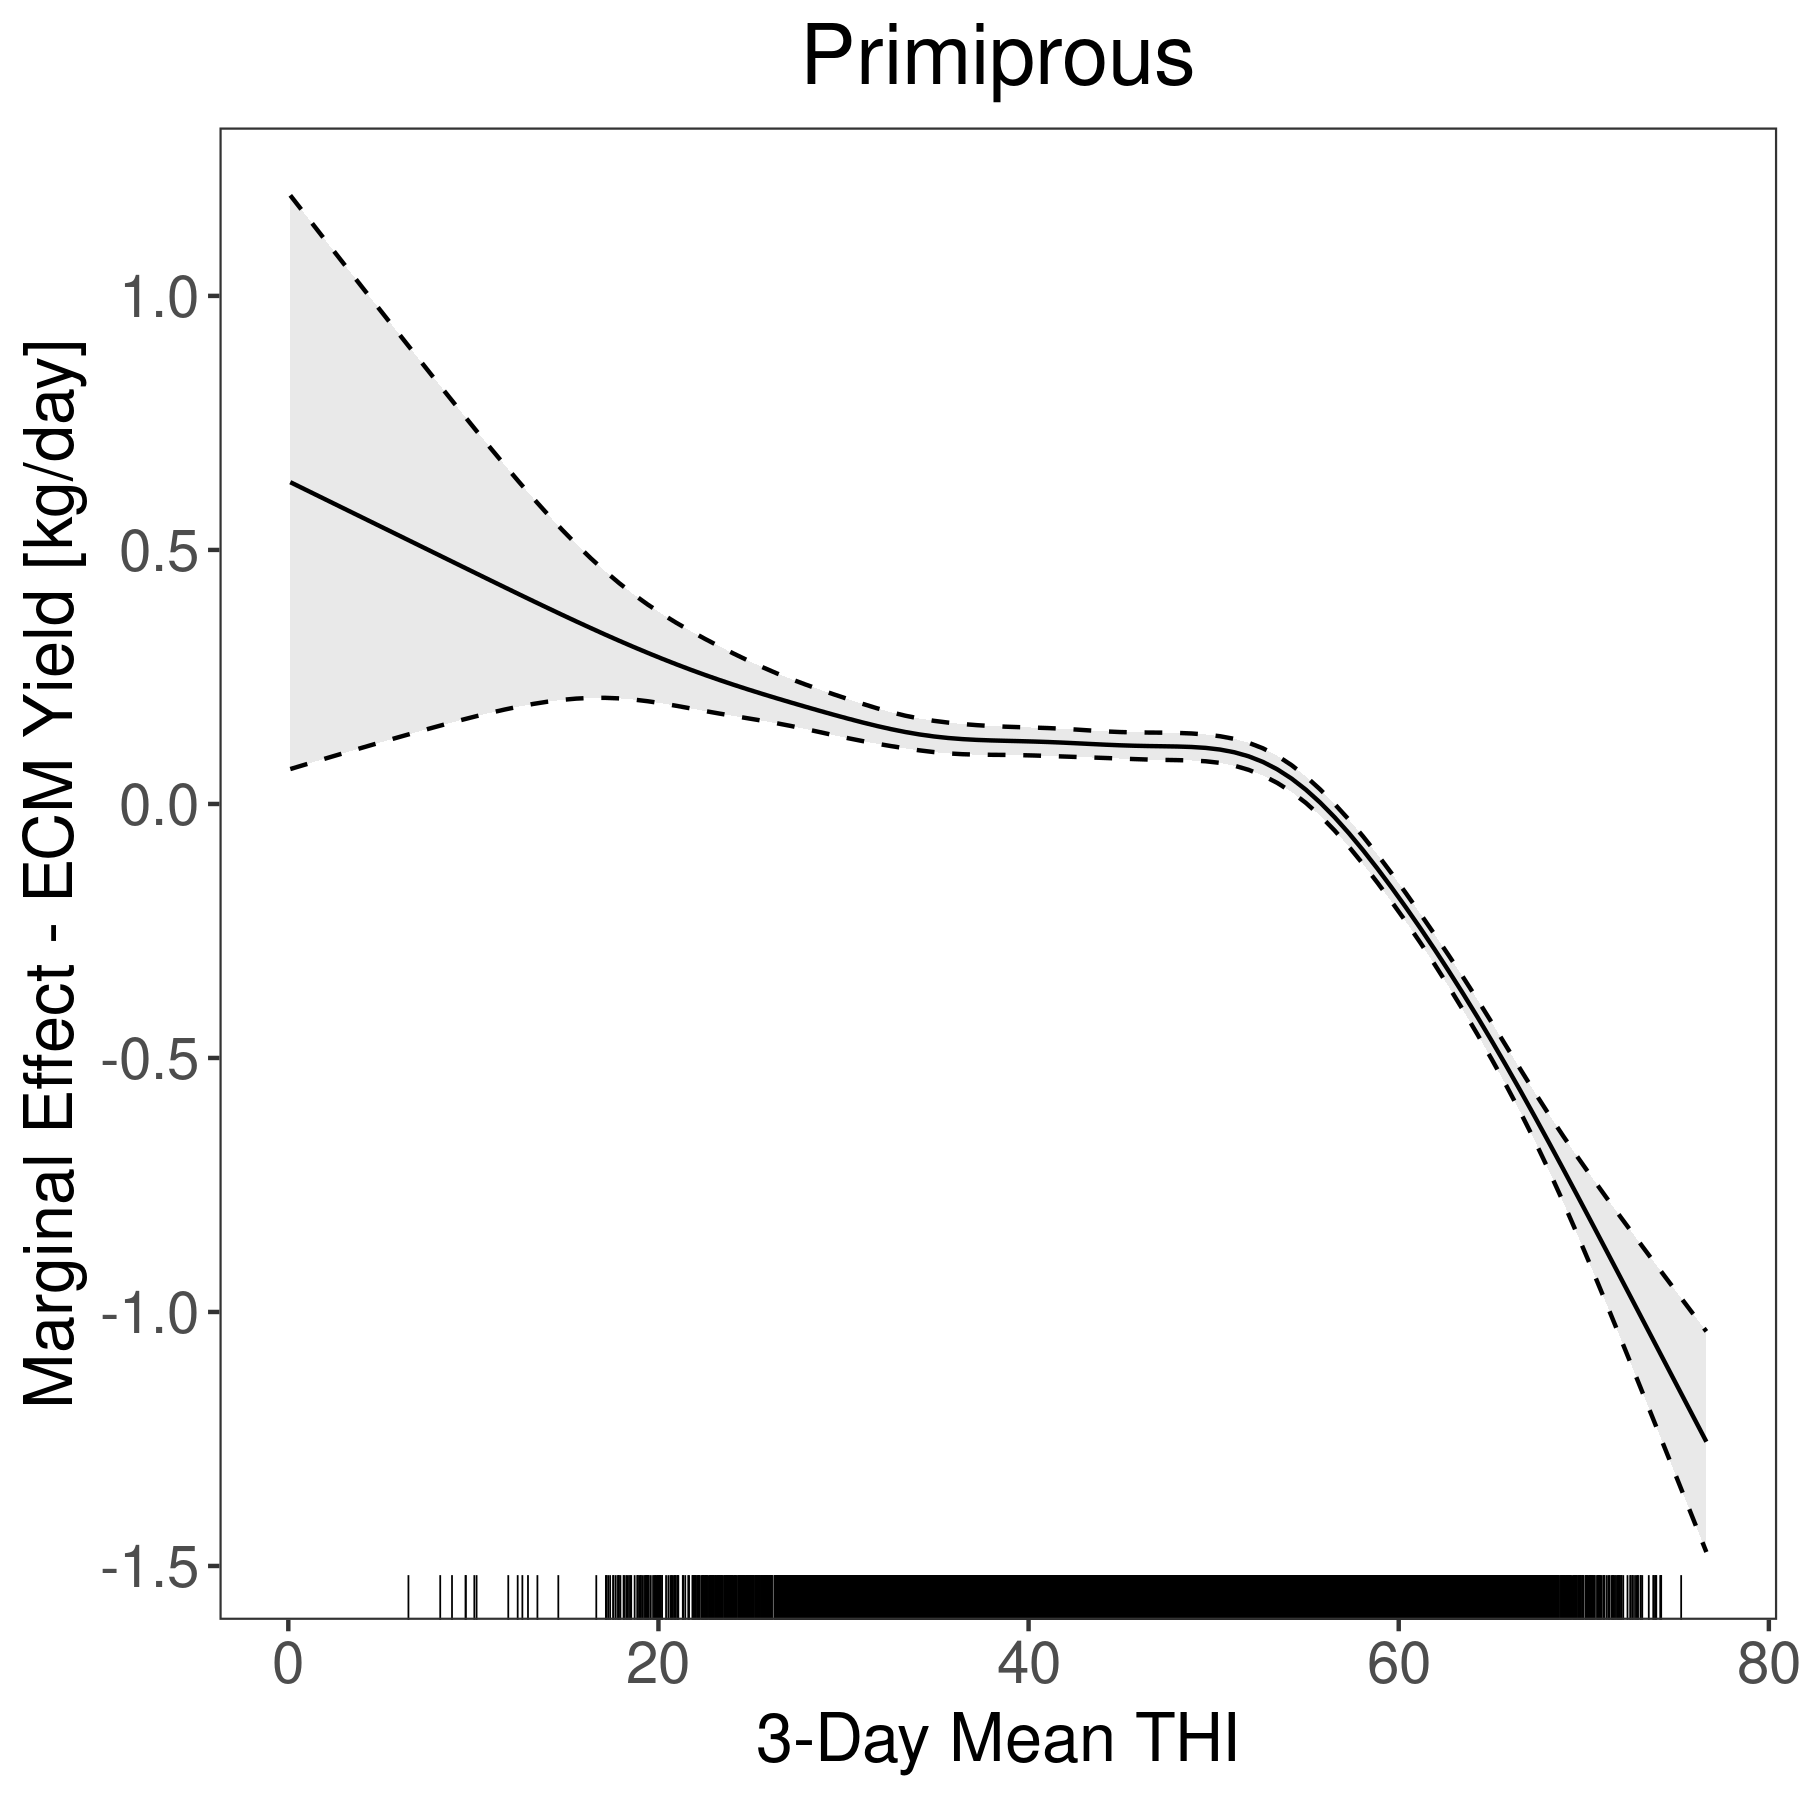
\includegraphics[width=\textwidth]{thesis/figures/models/ecm/full/sf_ecm_full/sf_ecm_full_marginal_thi_milk_primi.png}
    \end{subfigure}
    \hspace{0.05\textwidth} % Optional space between the figures
    \begin{subfigure}[b]{0.45\textwidth}
        \centering
        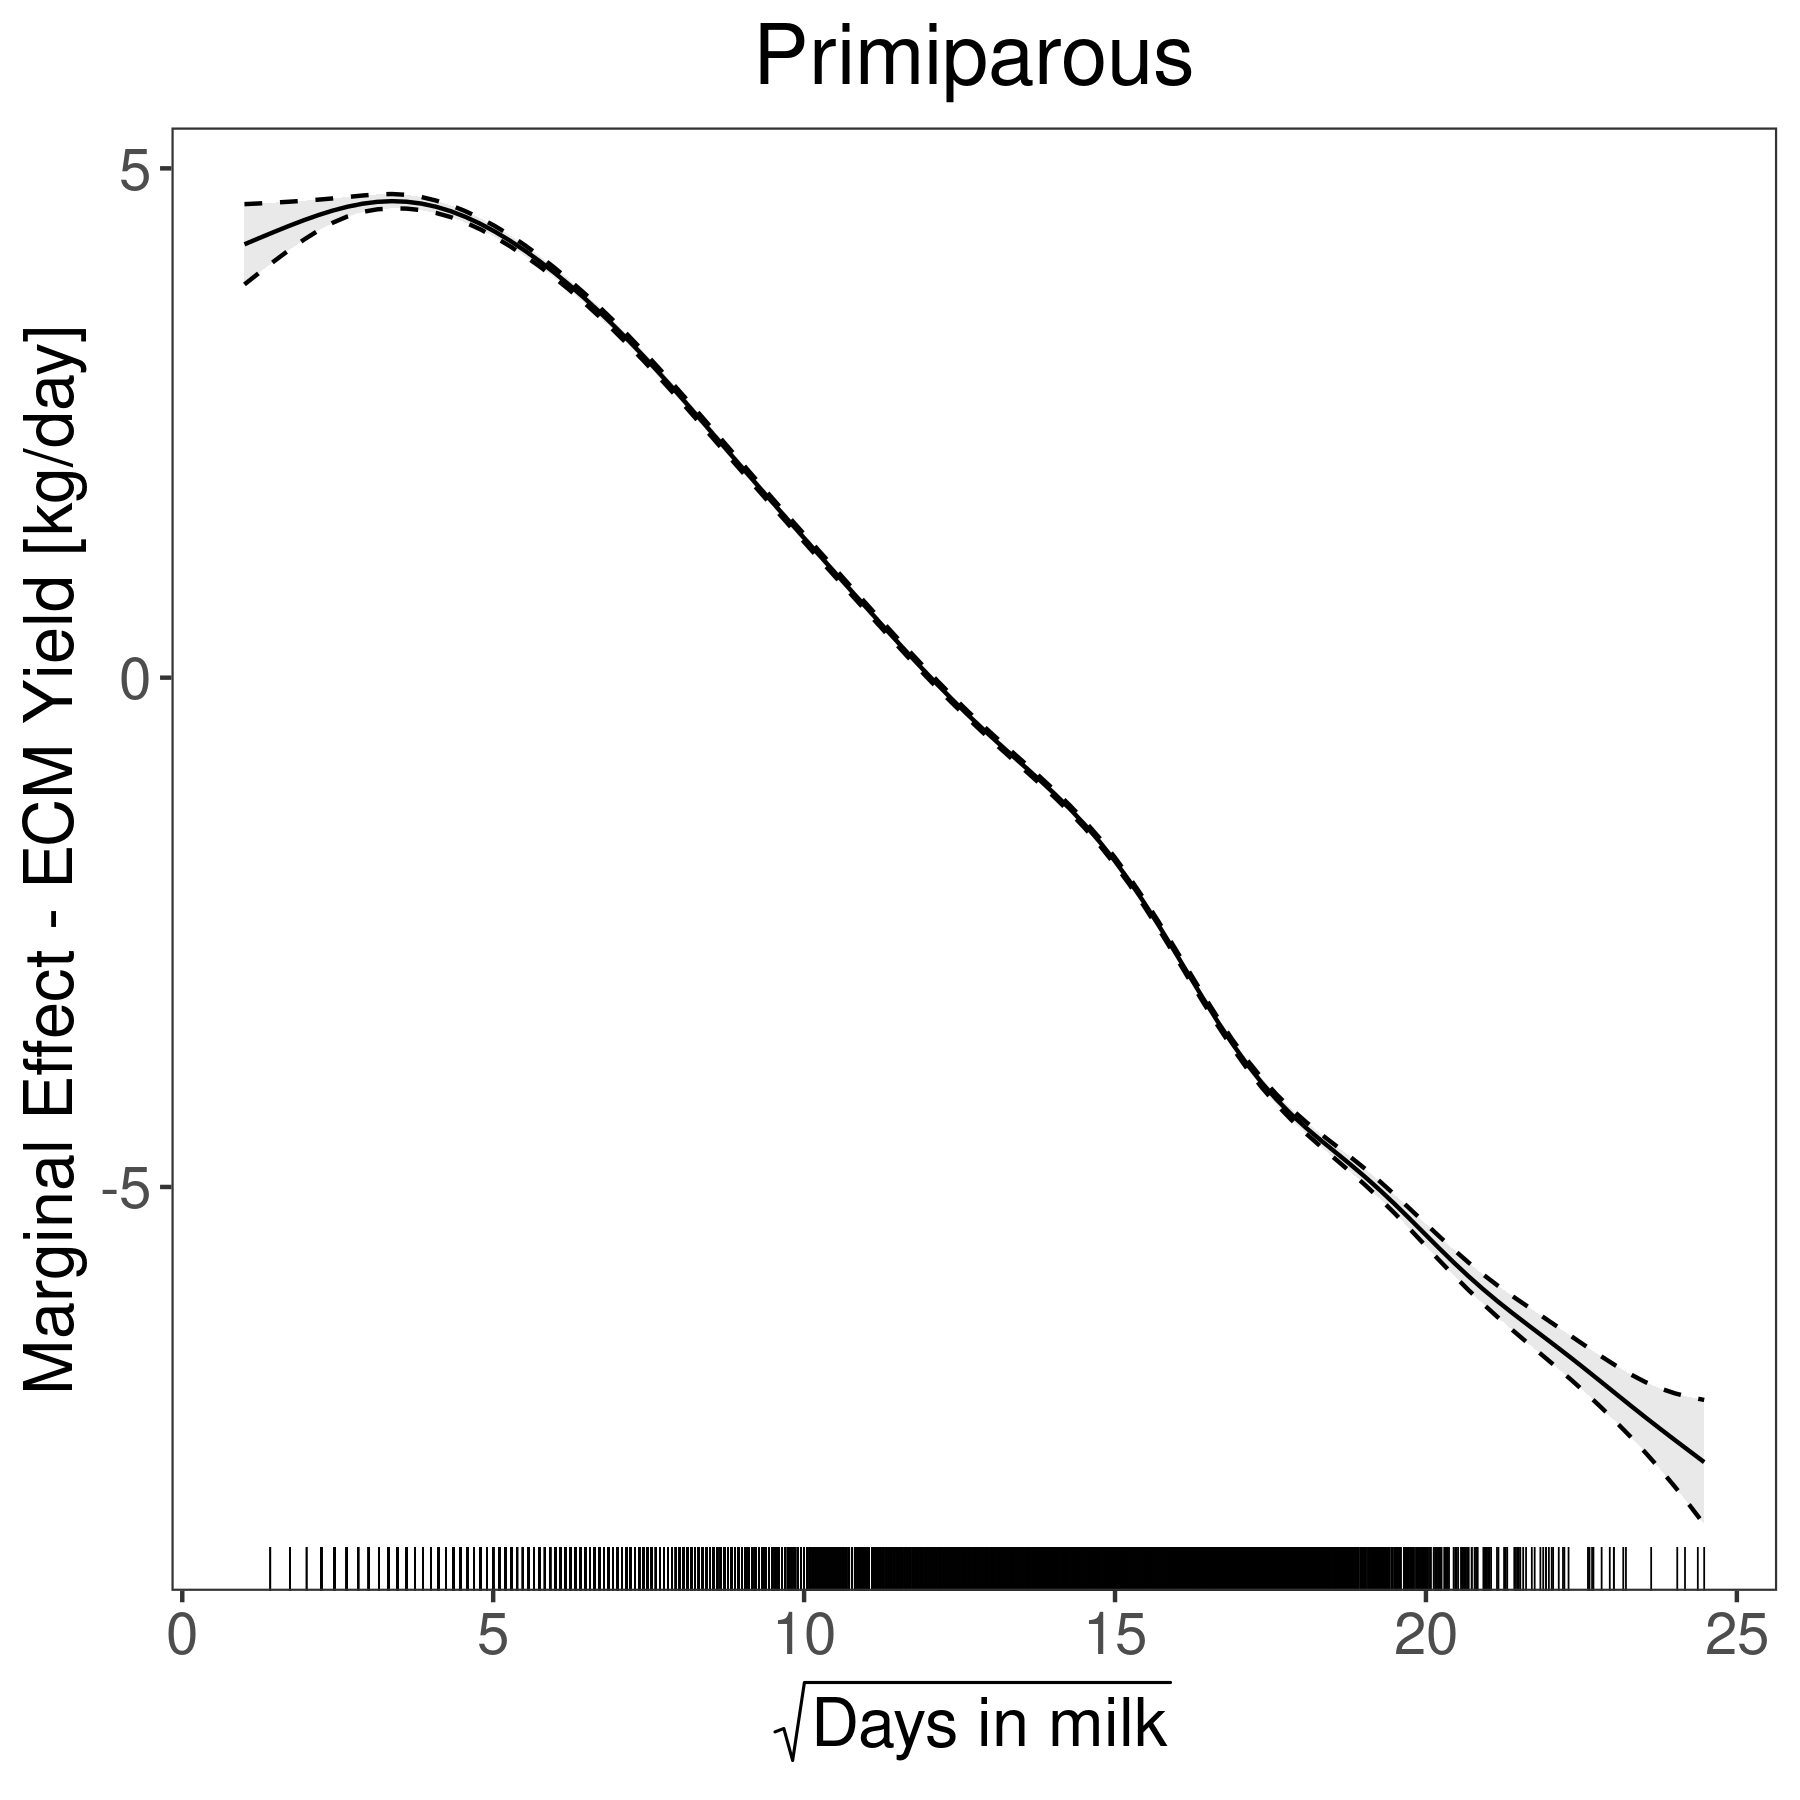
\includegraphics[width=\textwidth]{thesis/figures/models/ecm/full/sf_ecm_full/sf_ecm_full_marginal_dim_milk_primi.png}
    \end{subfigure}
    \begin{subfigure}[b]{0.45\textwidth}
        \centering
        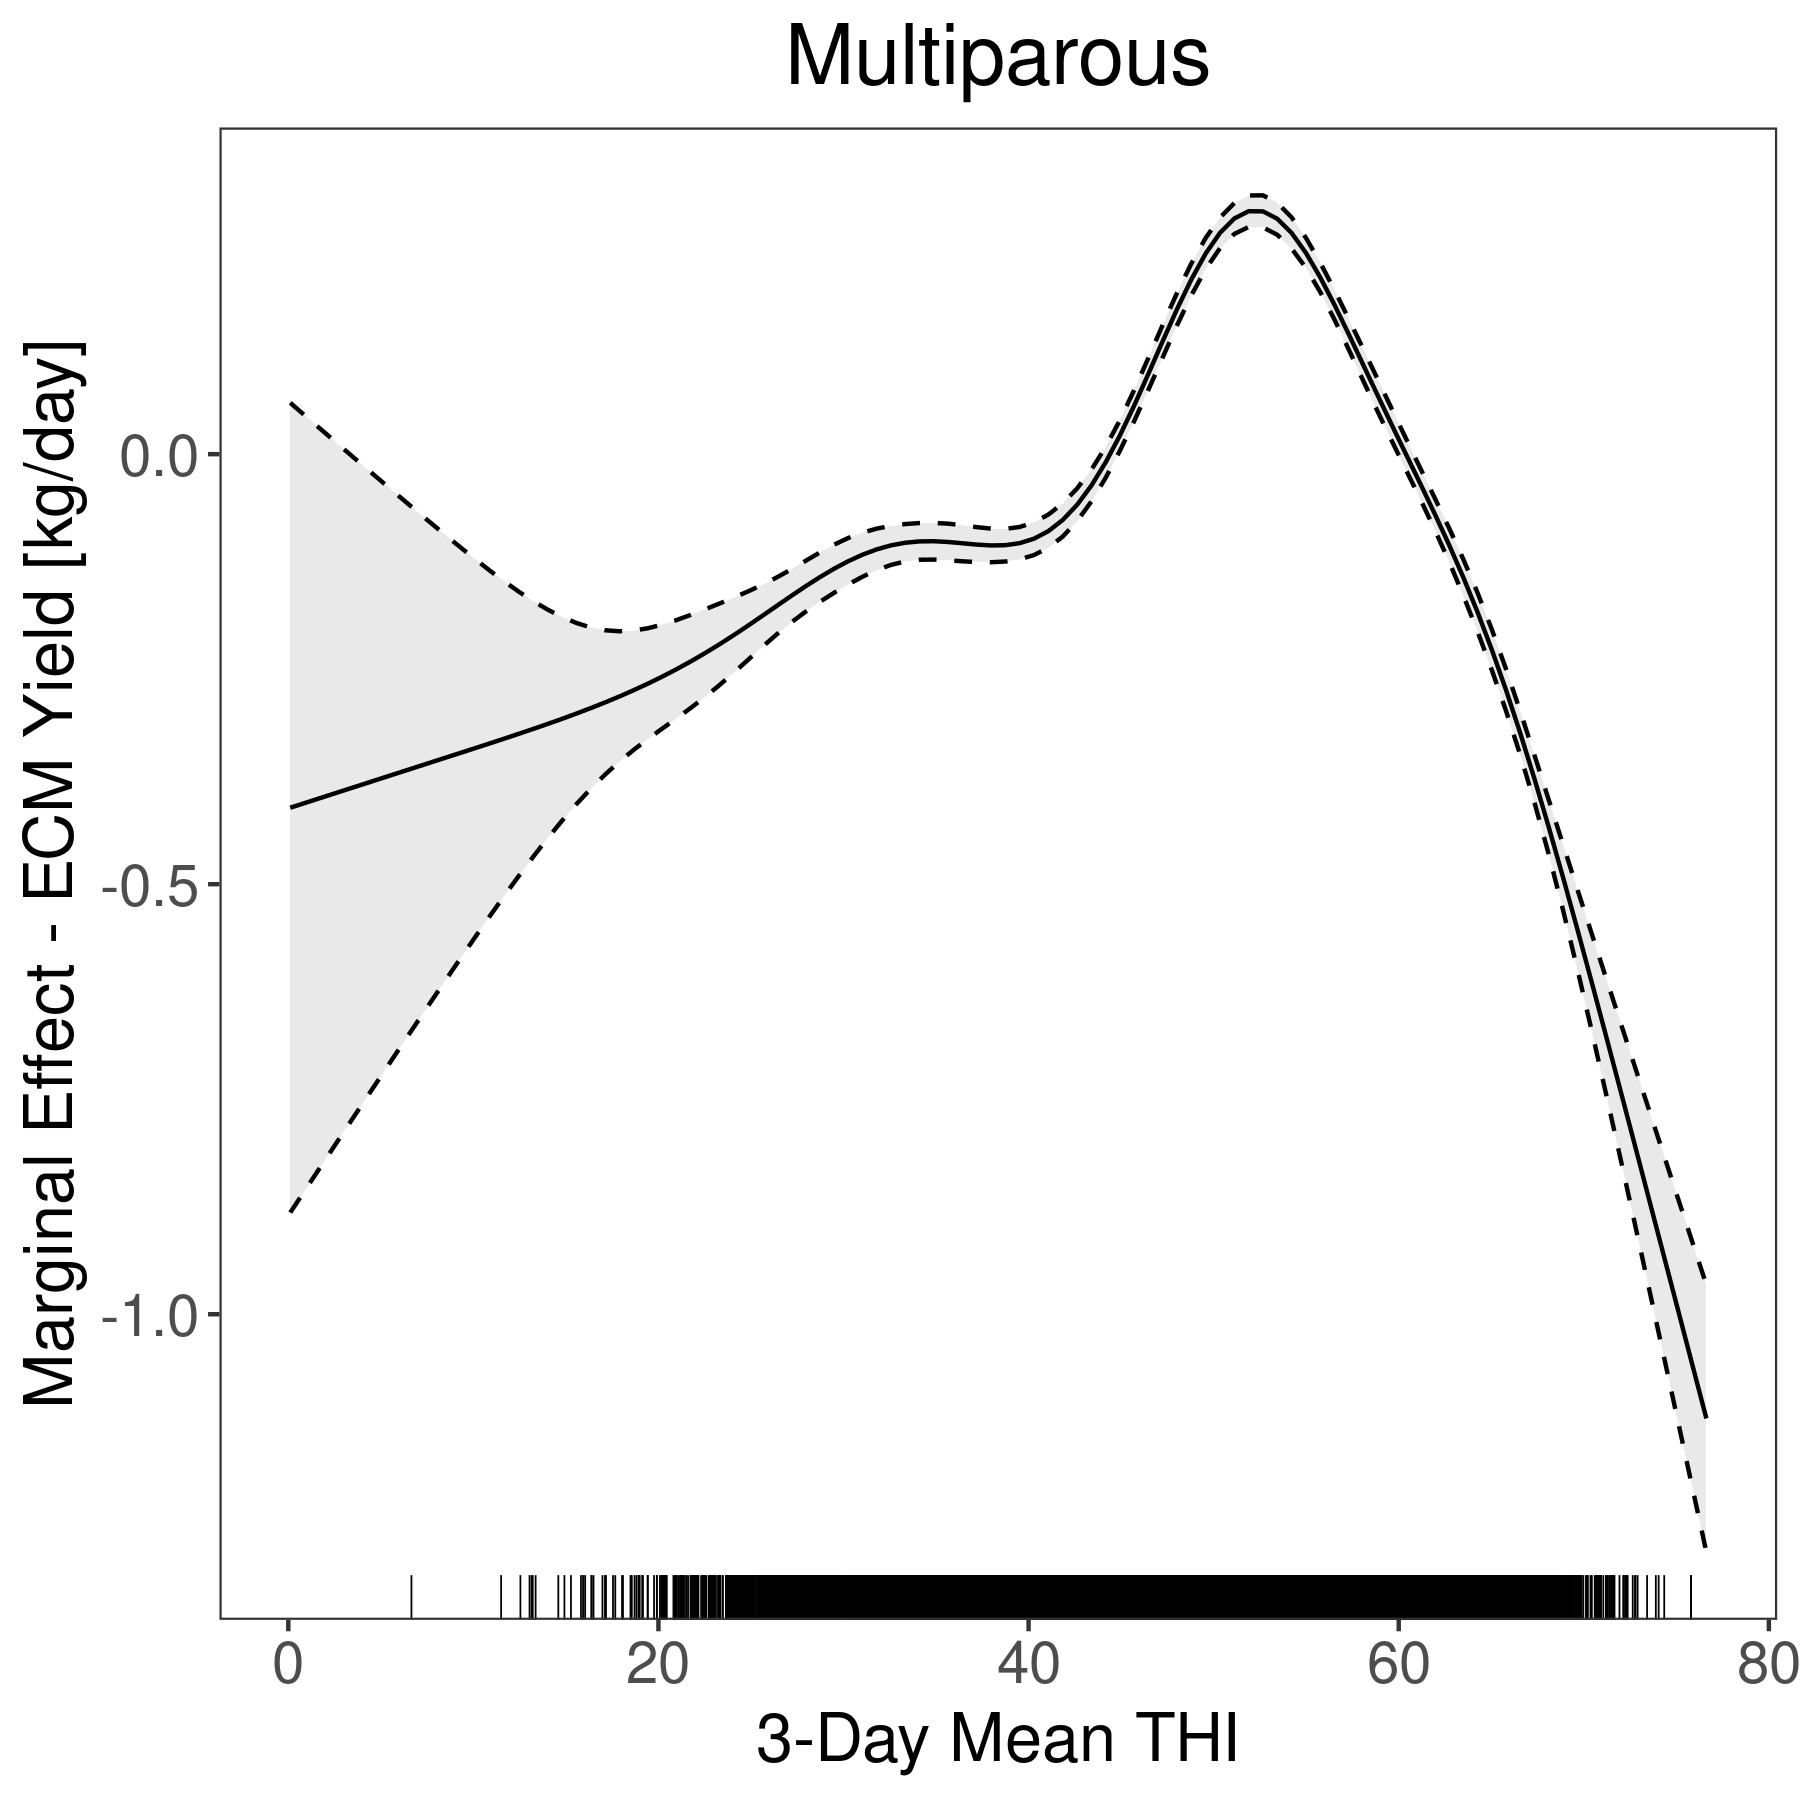
\includegraphics[width=\textwidth]{thesis/figures/models/ecm/full/sf_ecm_full/sf_ecm_full_marginal_thi_milk_multi.png}
    \end{subfigure}
    \hspace{0.05\textwidth} % Optional space between the figures
    \begin{subfigure}[b]{0.45\textwidth}
        \centering
        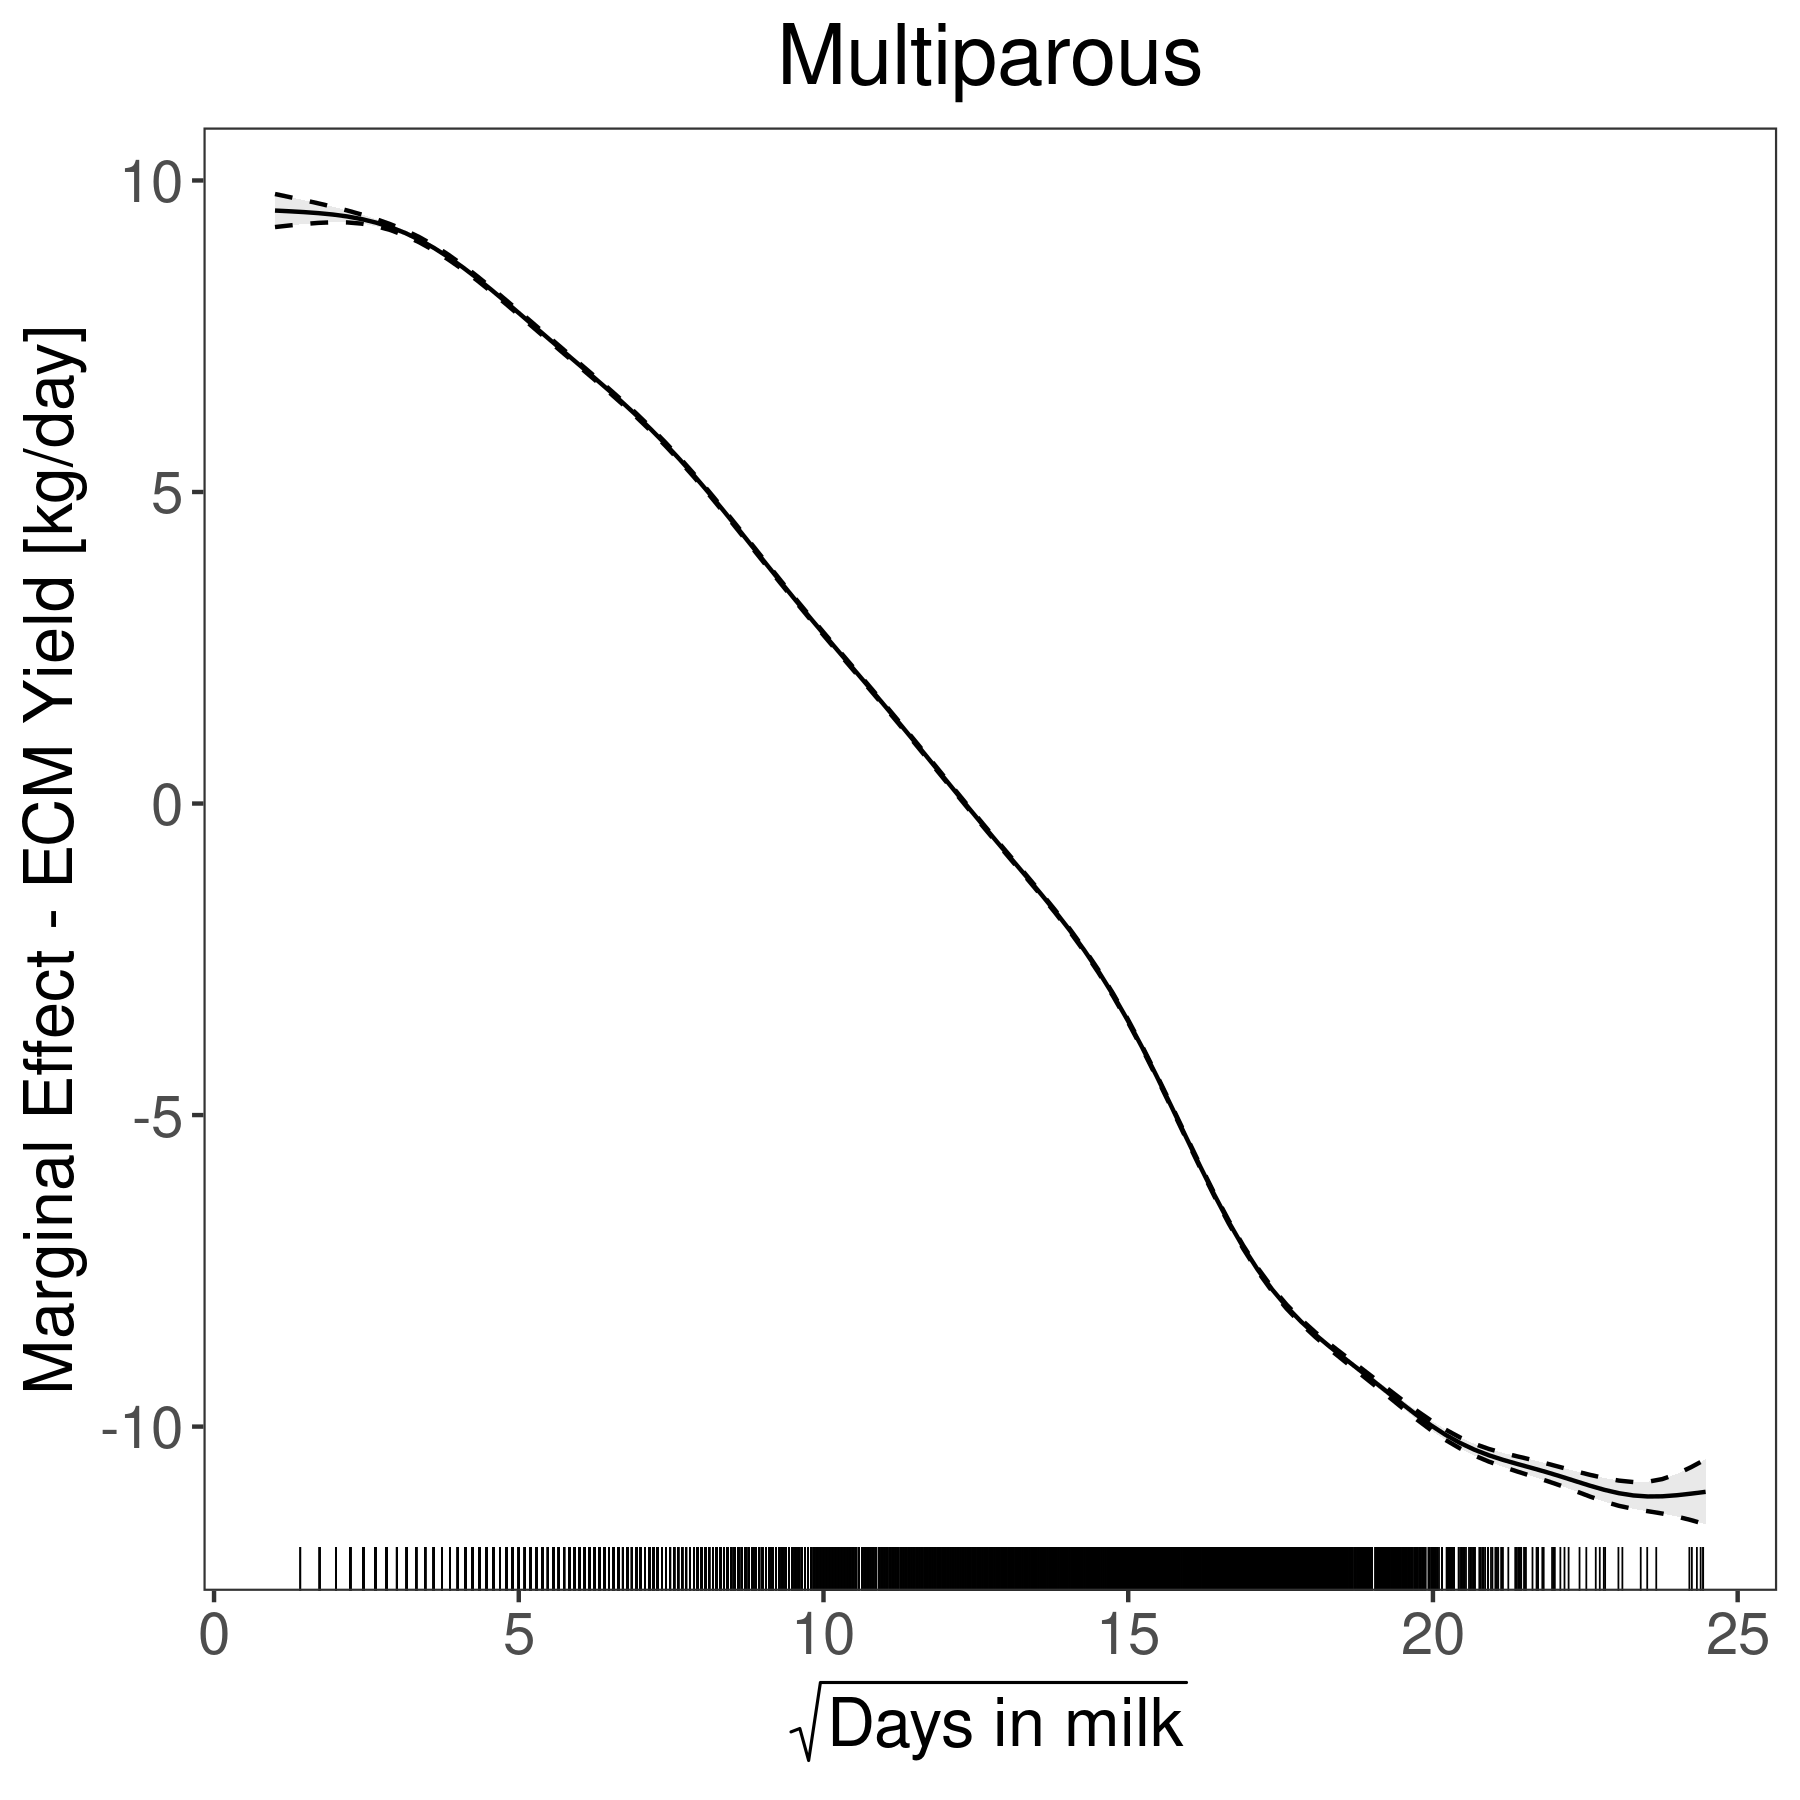
\includegraphics[width=\textwidth]{thesis/figures/models/ecm/full/sf_ecm_full/sf_ecm_full_marginal_dim_milk_multi.png}
    \end{subfigure}
    \caption[]{Swiss Fleckvieh: ECM Yield - 1984 - 2023 - THI Effect and Lactation Curve}
    \label{fig:main}
\end{figure}

\subsection{Split Period: Until 2010 - After 2010}
\addtocontents{toc}{\protect\setcounter{tocdepth}{-1}}
\subsubsection{Split Period: 1984 - 2010}\label{model:sf_ecm_before}

\paragraph{Model Summary} \quad \\

    \begin{table}[H]
    \centering
    \begin{tabular}{lrrrr}
    \textbf{A. parametric coefficients} & Estimate & Std. Error & t-value & p-value \\ 
       \hline
       \hline
      (Intercept) & 18.6574 & 0.3504 & 53.2489 & $<$ 0.0001 \\ 
      parityprimiparous & -3.1387 & 0.0130 & -242.3247 & $<$ 0.0001 \\ 
      year1985 & 0.5924 & 0.1977 & 2.9963 & 0.0027 \\ 
      year1986 & 0.5314 & 0.2944 & 1.8051 & 0.0711 \\ 
      year1987 & 0.2646 & 0.3287 & 0.8049 & 0.4209 \\ 
      year1988 & -0.0889 & 0.3543 & -0.2510 & 0.8018 \\ 
      year1989 & 0.7936 & 0.3810 & 2.0827 & 0.0373 \\ 
      year1990 & 1.2909 & 0.3896 & 3.3139 & 0.0009 \\ 
      year1991 & 1.5349 & 0.3928 & 3.9080 & 0.0001 \\ 
      year1992 & 1.8697 & 0.3991 & 4.6853 & $<$ 0.0001 \\ 
      year1993 & 1.7970 & 0.3757 & 4.7832 & $<$ 0.0001 \\ 
      year1994 & 1.6346 & 0.3831 & 4.2672 & $<$ 0.0001 \\ 
      year1995 & 1.9864 & 0.3616 & 5.4932 & $<$ 0.0001 \\ 
      year1996 & 2.2906 & 0.3599 & 6.3642 & $<$ 0.0001 \\ 
      year1997 & 2.8227 & 0.3546 & 7.9605 & $<$ 0.0001 \\ 
      year1998 & 3.7164 & 0.4462 & 8.3282 & $<$ 0.0001 \\ 
      year1999 & 3.7134 & 0.4226 & 8.7877 & $<$ 0.0001 \\ 
      year2000 & 3.6881 & 0.4271 & 8.6353 & $<$ 0.0001 \\ 
      year2001 & 4.0909 & 0.4333 & 9.4403 & $<$ 0.0001 \\ 
      year2002 & 4.1925 & 0.4333 & 9.6762 & $<$ 0.0001 \\ 
      year2003 & 4.7166 & 0.4412 & 10.6903 & $<$ 0.0001 \\ 
      year2004 & 5.3342 & 0.4443 & 12.0070 & $<$ 0.0001 \\ 
      year2005 & 5.8354 & 0.4797 & 12.1651 & $<$ 0.0001 \\ 
      year2006 & 5.8436 & 0.4795 & 12.1875 & $<$ 0.0001 \\ 
      year2007 & 5.5932 & 0.4985 & 11.2199 & $<$ 0.0001 \\ 
      year2008 & 5.9158 & 0.5046 & 11.7229 & $<$ 0.0001 \\ 
      year2009 & 6.4499 & 0.5281 & 12.2140 & $<$ 0.0001 \\ 
      year2010 & 7.1064 & 0.7553 & 9.4092 & $<$ 0.0001 \\ 
       \hline
    \textbf{B. smooth terms} & edf & Ref.df & F-value & p-value \\ 
    \hline
    \hline
      s(thi\_mean\_t0\_3d):paritymultiparous & 8.6994 & 8.6994 & 314.1151 & $<$ 0.0001 \\ 
      s(thi\_mean\_t0\_3d):parityprimiparous & 7.1424 & 7.1424 & 143.5337 & $<$ 0.0001 \\ 
      s(days\_in\_milk\_t):paritymultiparous & 13.5087 & 13.5087 & 161236.6570 & $<$ 0.0001 \\ 
      s(days\_in\_milk\_t):parityprimiparous & 12.1975 & 12.1975 & 14112.6321 & $<$ 0.0001 \\ 
       \hline
    \end{tabular}
    \caption[]{Swiss Fleckvieh: ECM Yield - 1984-2010 - GAMM model summary without random effect terms.}
    \end{table}

\newpage
\begin{table}[H]
\centering
\begin{tabular}
{l | r | r | r | r}
\textbf{Smooth Term Fixed Effect} & Est. & SE & z & p\\
\hline
\hline
s(thi\_mean\_t0\_3d):multiFx1 & 0.4342 & 0.0866 & 5.01 & $<$ 1e-06\\
s(thi\_mean\_t0\_3d):primiFx1 & 0.4046 & 0.1067 & 3.79 & 0.0002\\
s(days\_in\_milk\_):multiFx1 & -0.5972 & 0.4296 & -1.39 & 0.1645\\
s(days\_in\_milk\_):primiFx1 & -0.5188 & 0.4339 & -1.20 & 0.2319\\
\hline
\textbf{Variance Component} & Estimated $\sigma$ & & & \\
\hline
\hline
$\sigma_\alpha$ & 2.6516 & & & \\
$\sigma_\iota$ & 0.9288 & & & \\
$\sigma_\phi$ & 2.9589 & & & \\
s(thi\_mean\_t0\_3d):multi & 2.5013 & & & \\
s(days\_in\_milk\_):primi & 3.8774 & & & \\
s(days\_in\_milk\_):multi & 7.1478 & & & \\
s(thi\_mean\_t0\_3d):primi & 1.2666 & & & \\
Residual & 3.2839 & & & \\
\end{tabular}
\caption[]{Swiss Fleckvieh: ECM Yield - 1984-2010 - Mixed Model Summary - Smooth Terms and Random Effects.}
\end{table}

\paragraph{Model Diagnostics} \quad \\
\begin{figure}[H]
    \centering
    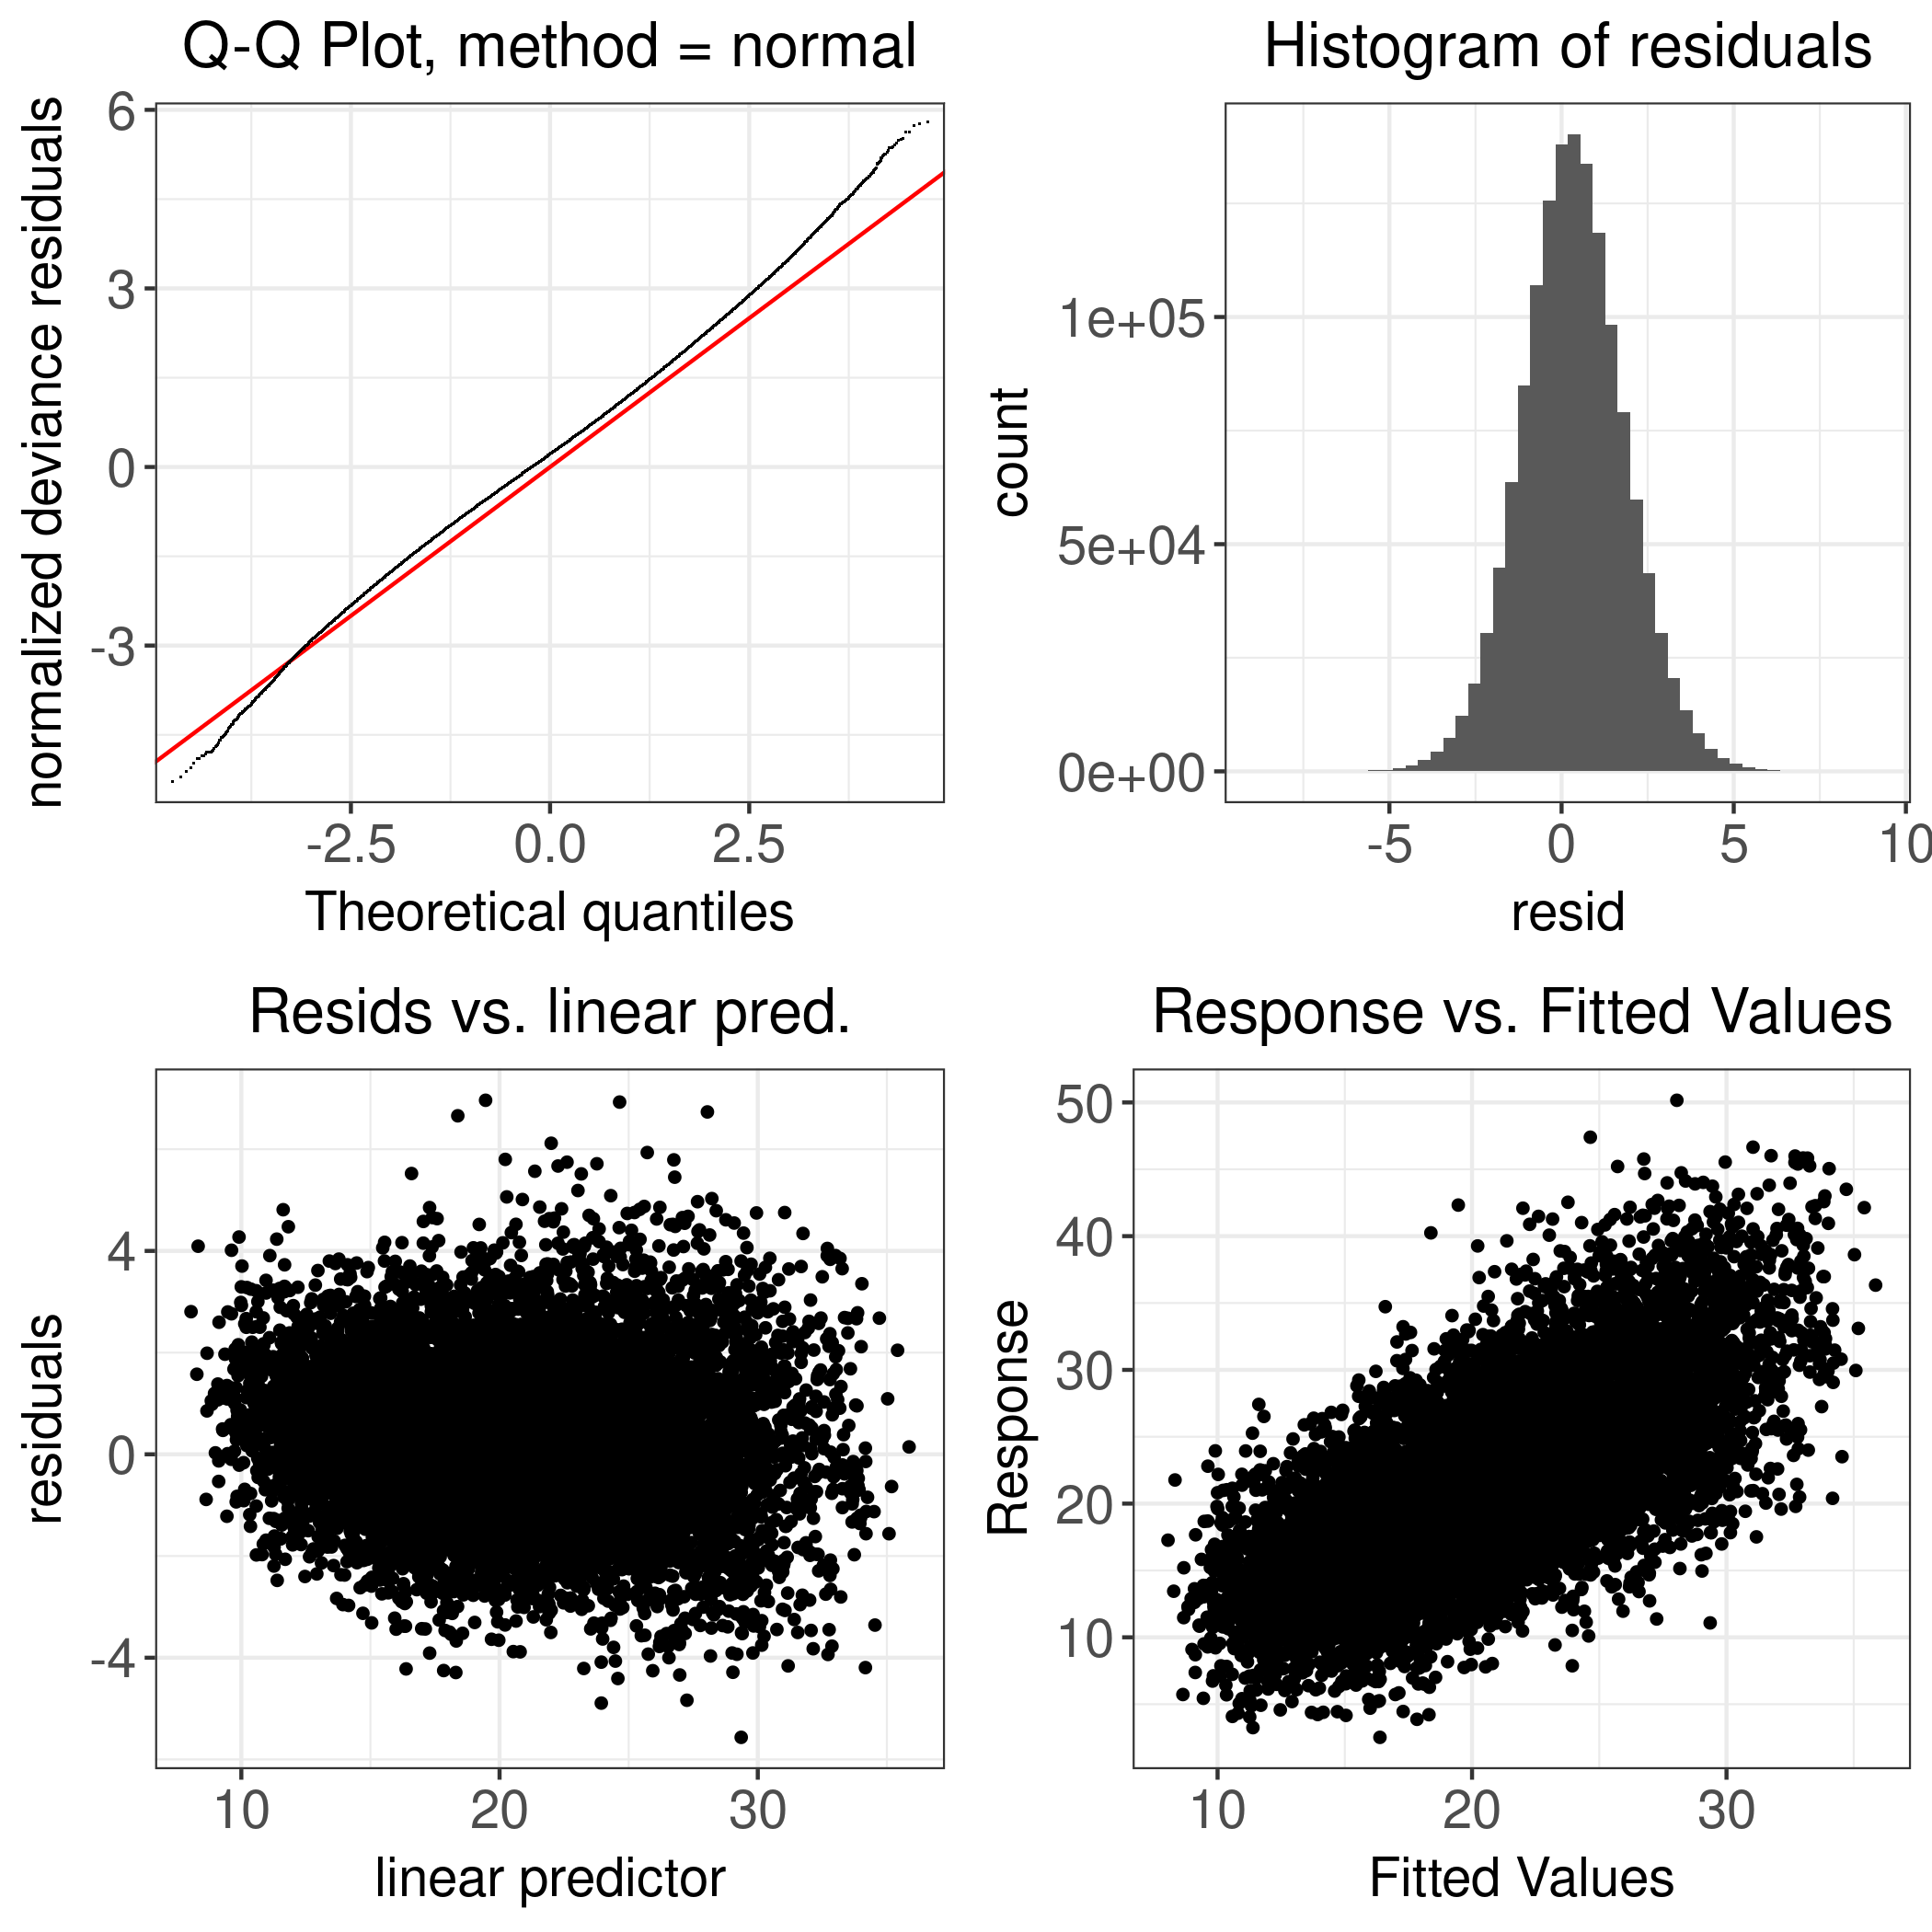
\includegraphics[width=0.6\textwidth]{thesis/figures/models/ecm/before2010/sf_ecm_before2010/sf_ecm_before2010_diagnostics.png}
    \caption[]{Swiss Fleckvieh: ECM Yield - 1984-2010 - Diagnostic Plot}
\end{figure}

\newpage
\paragraph{THI Effect and Lactation Curve} \quad \\
\begin{figure}[H]
    \centering
    \begin{subfigure}[b]{0.45\textwidth}
        \centering
        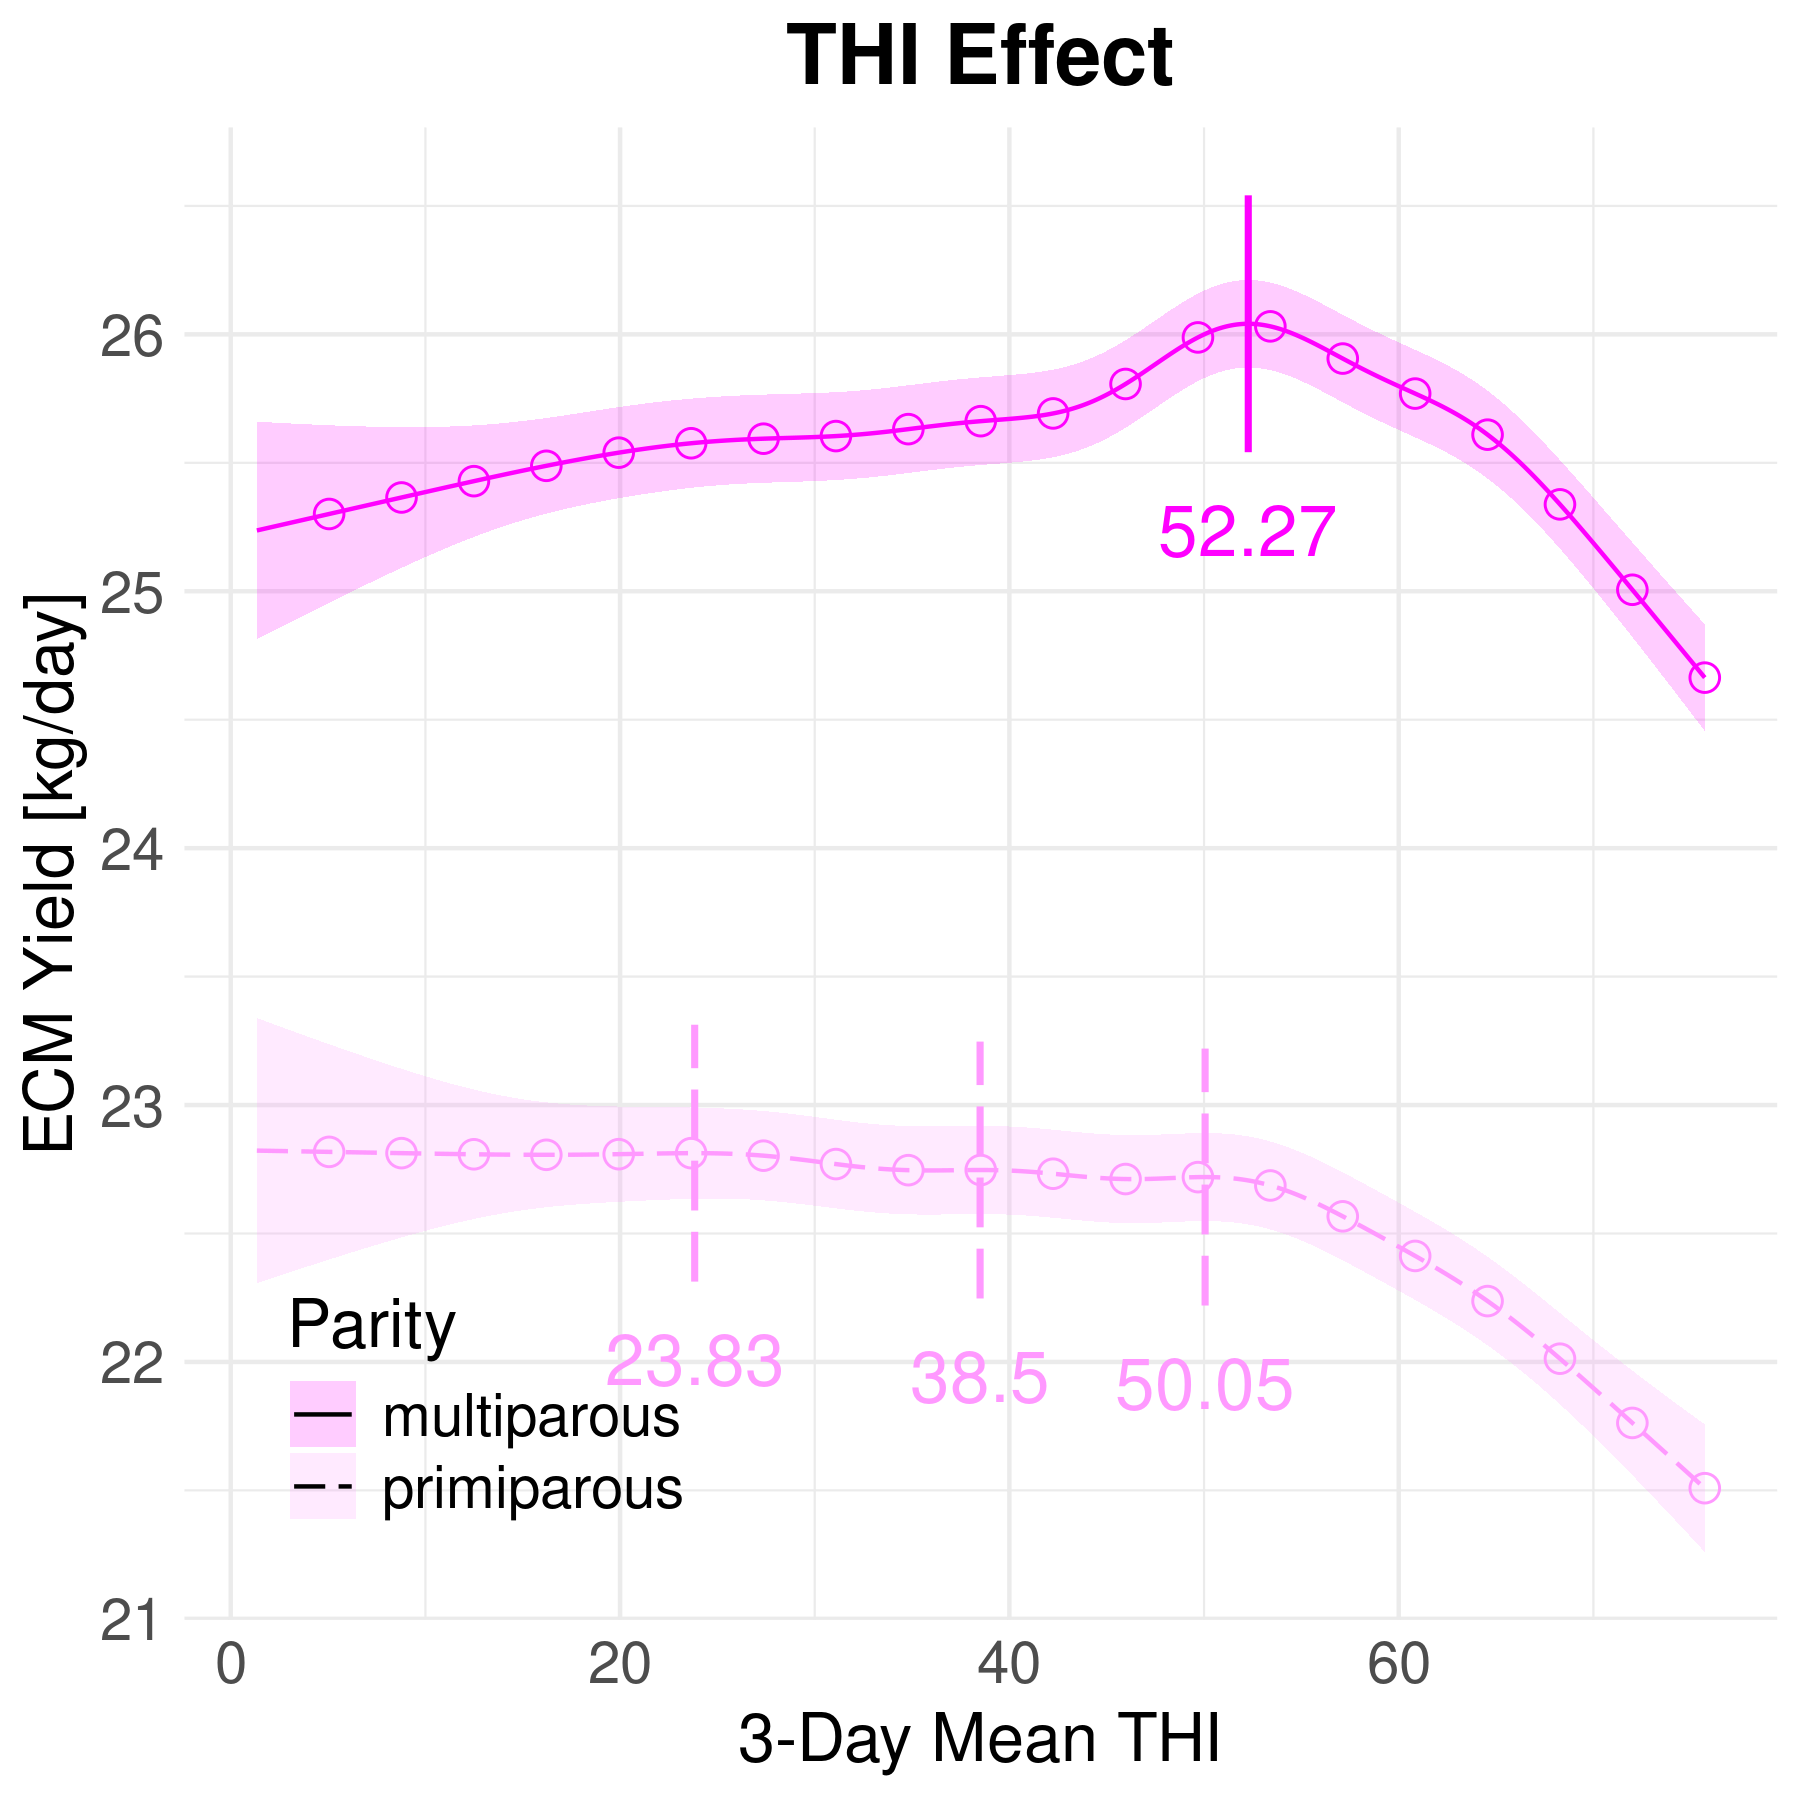
\includegraphics[width=\textwidth]{thesis/figures/models/ecm/before2010/sf_ecm_before2010/sf_ecm_before2010_marginal_thi_milk_combined.png}
    \end{subfigure}
    \hspace{0.05\textwidth} % Optional space between the figures
    \begin{subfigure}[b]{0.45\textwidth}
        \centering
        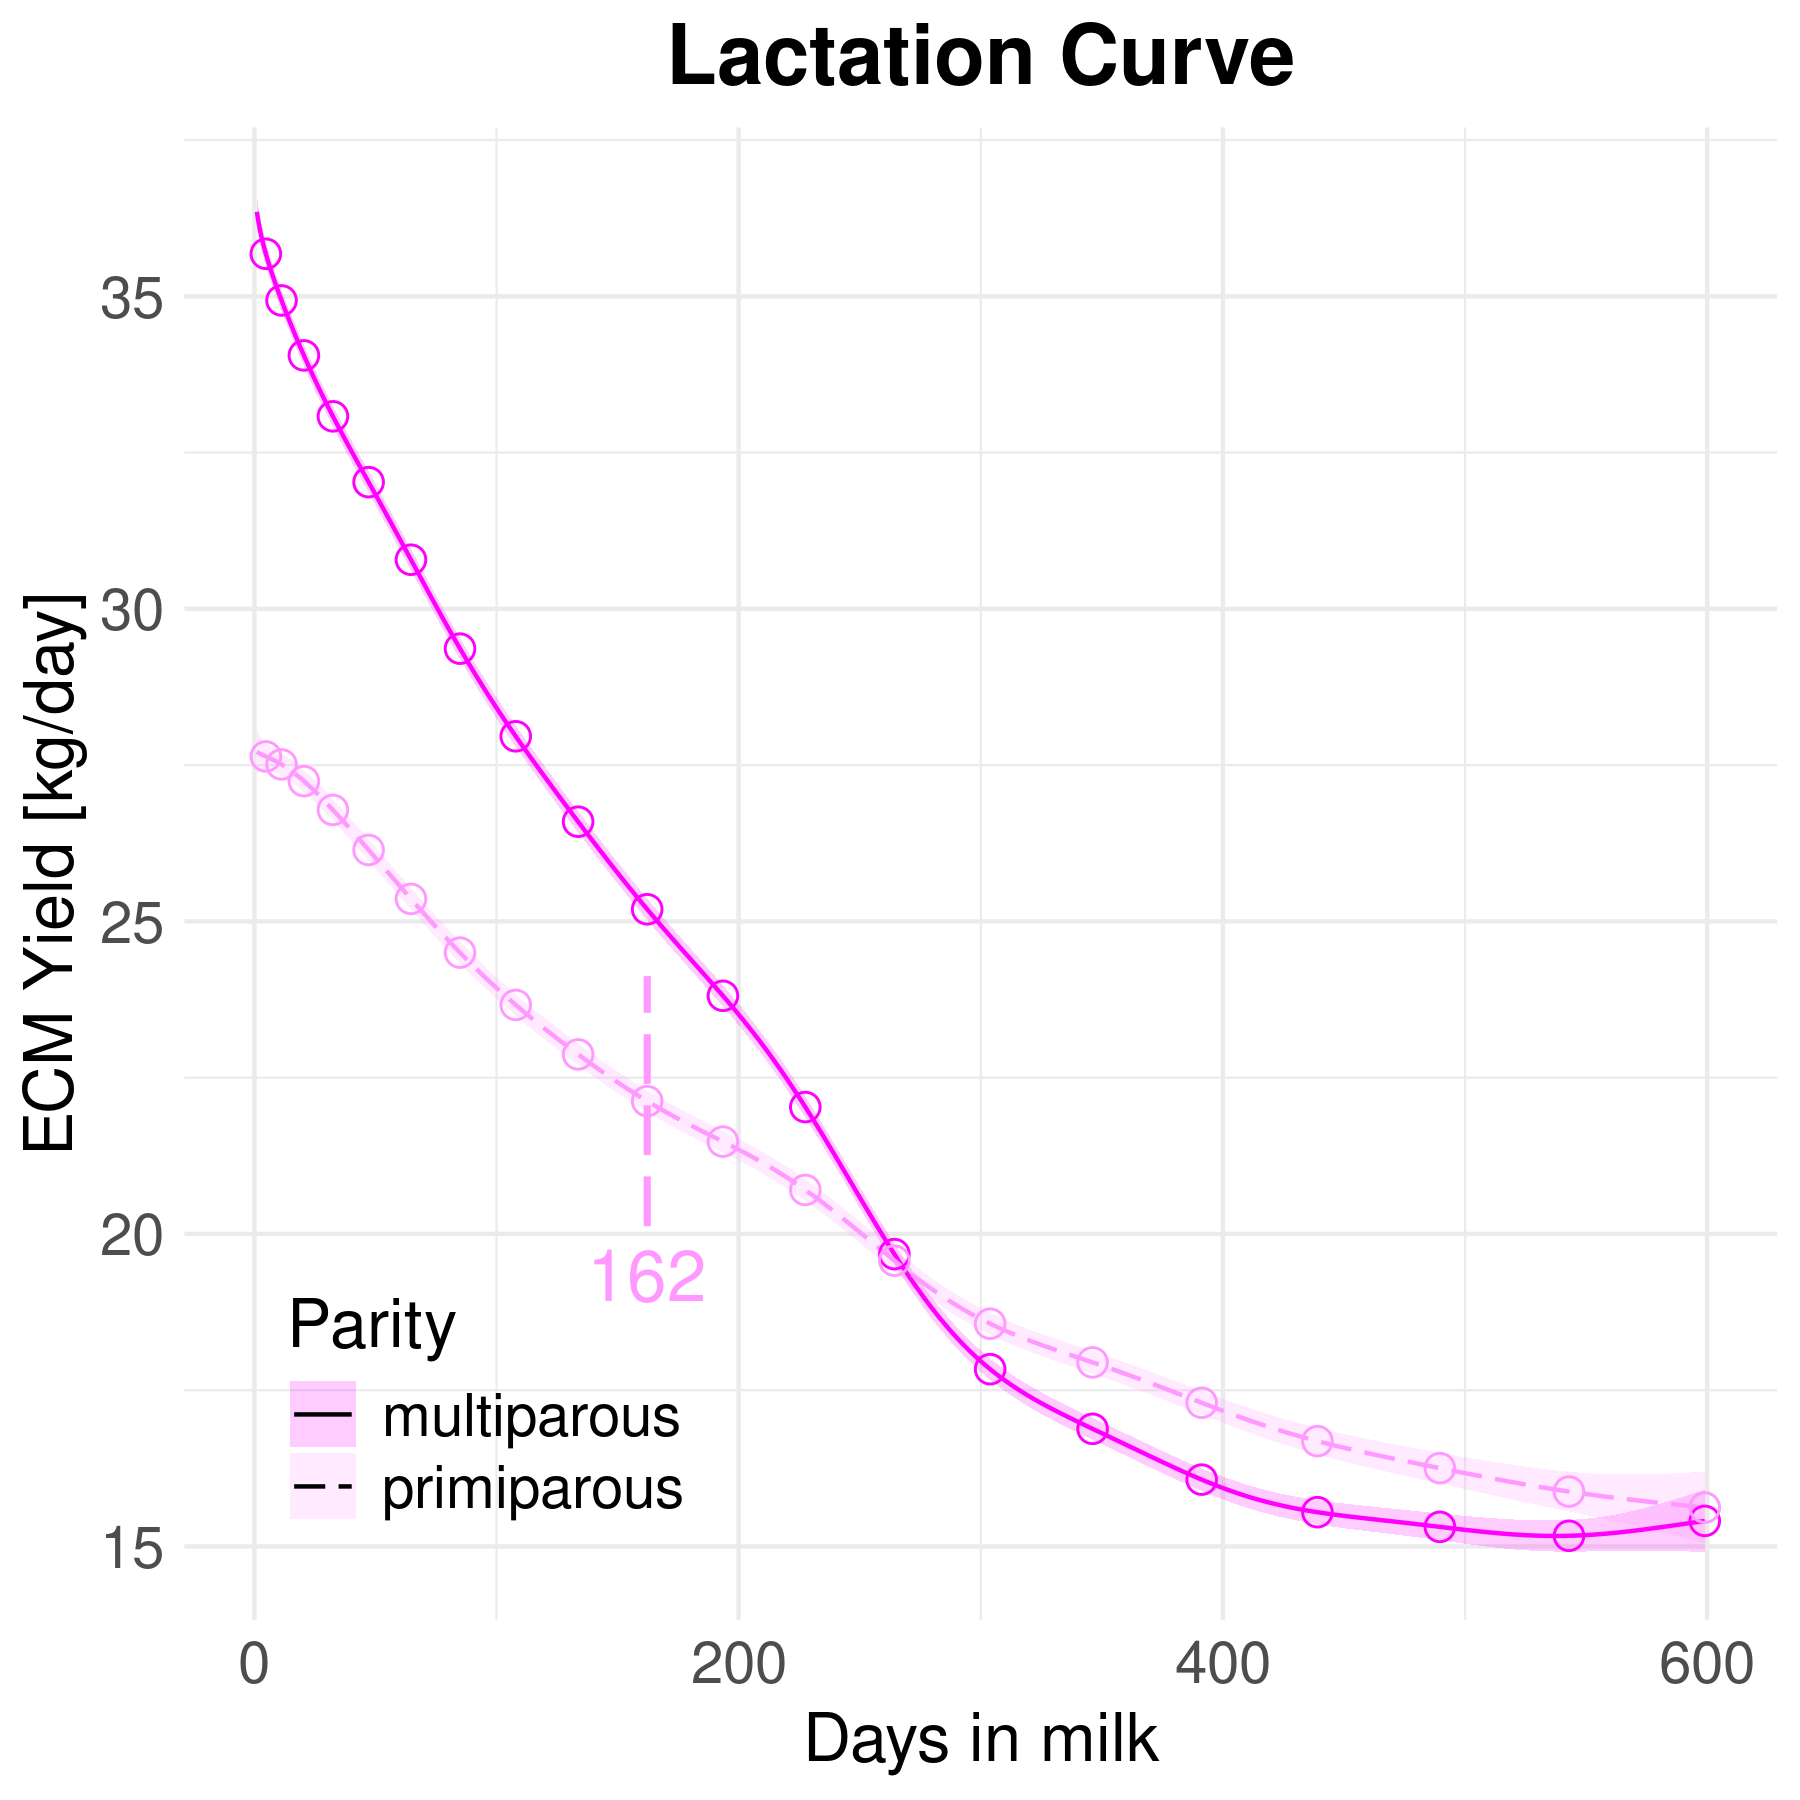
\includegraphics[width=\textwidth]{thesis/figures/models/ecm/before2010/sf_ecm_before2010/sf_ecm_before2010_marginal_dim_milk_combined.png}
    \end{subfigure}
    \begin{subfigure}[b]{0.45\textwidth}
        \centering
        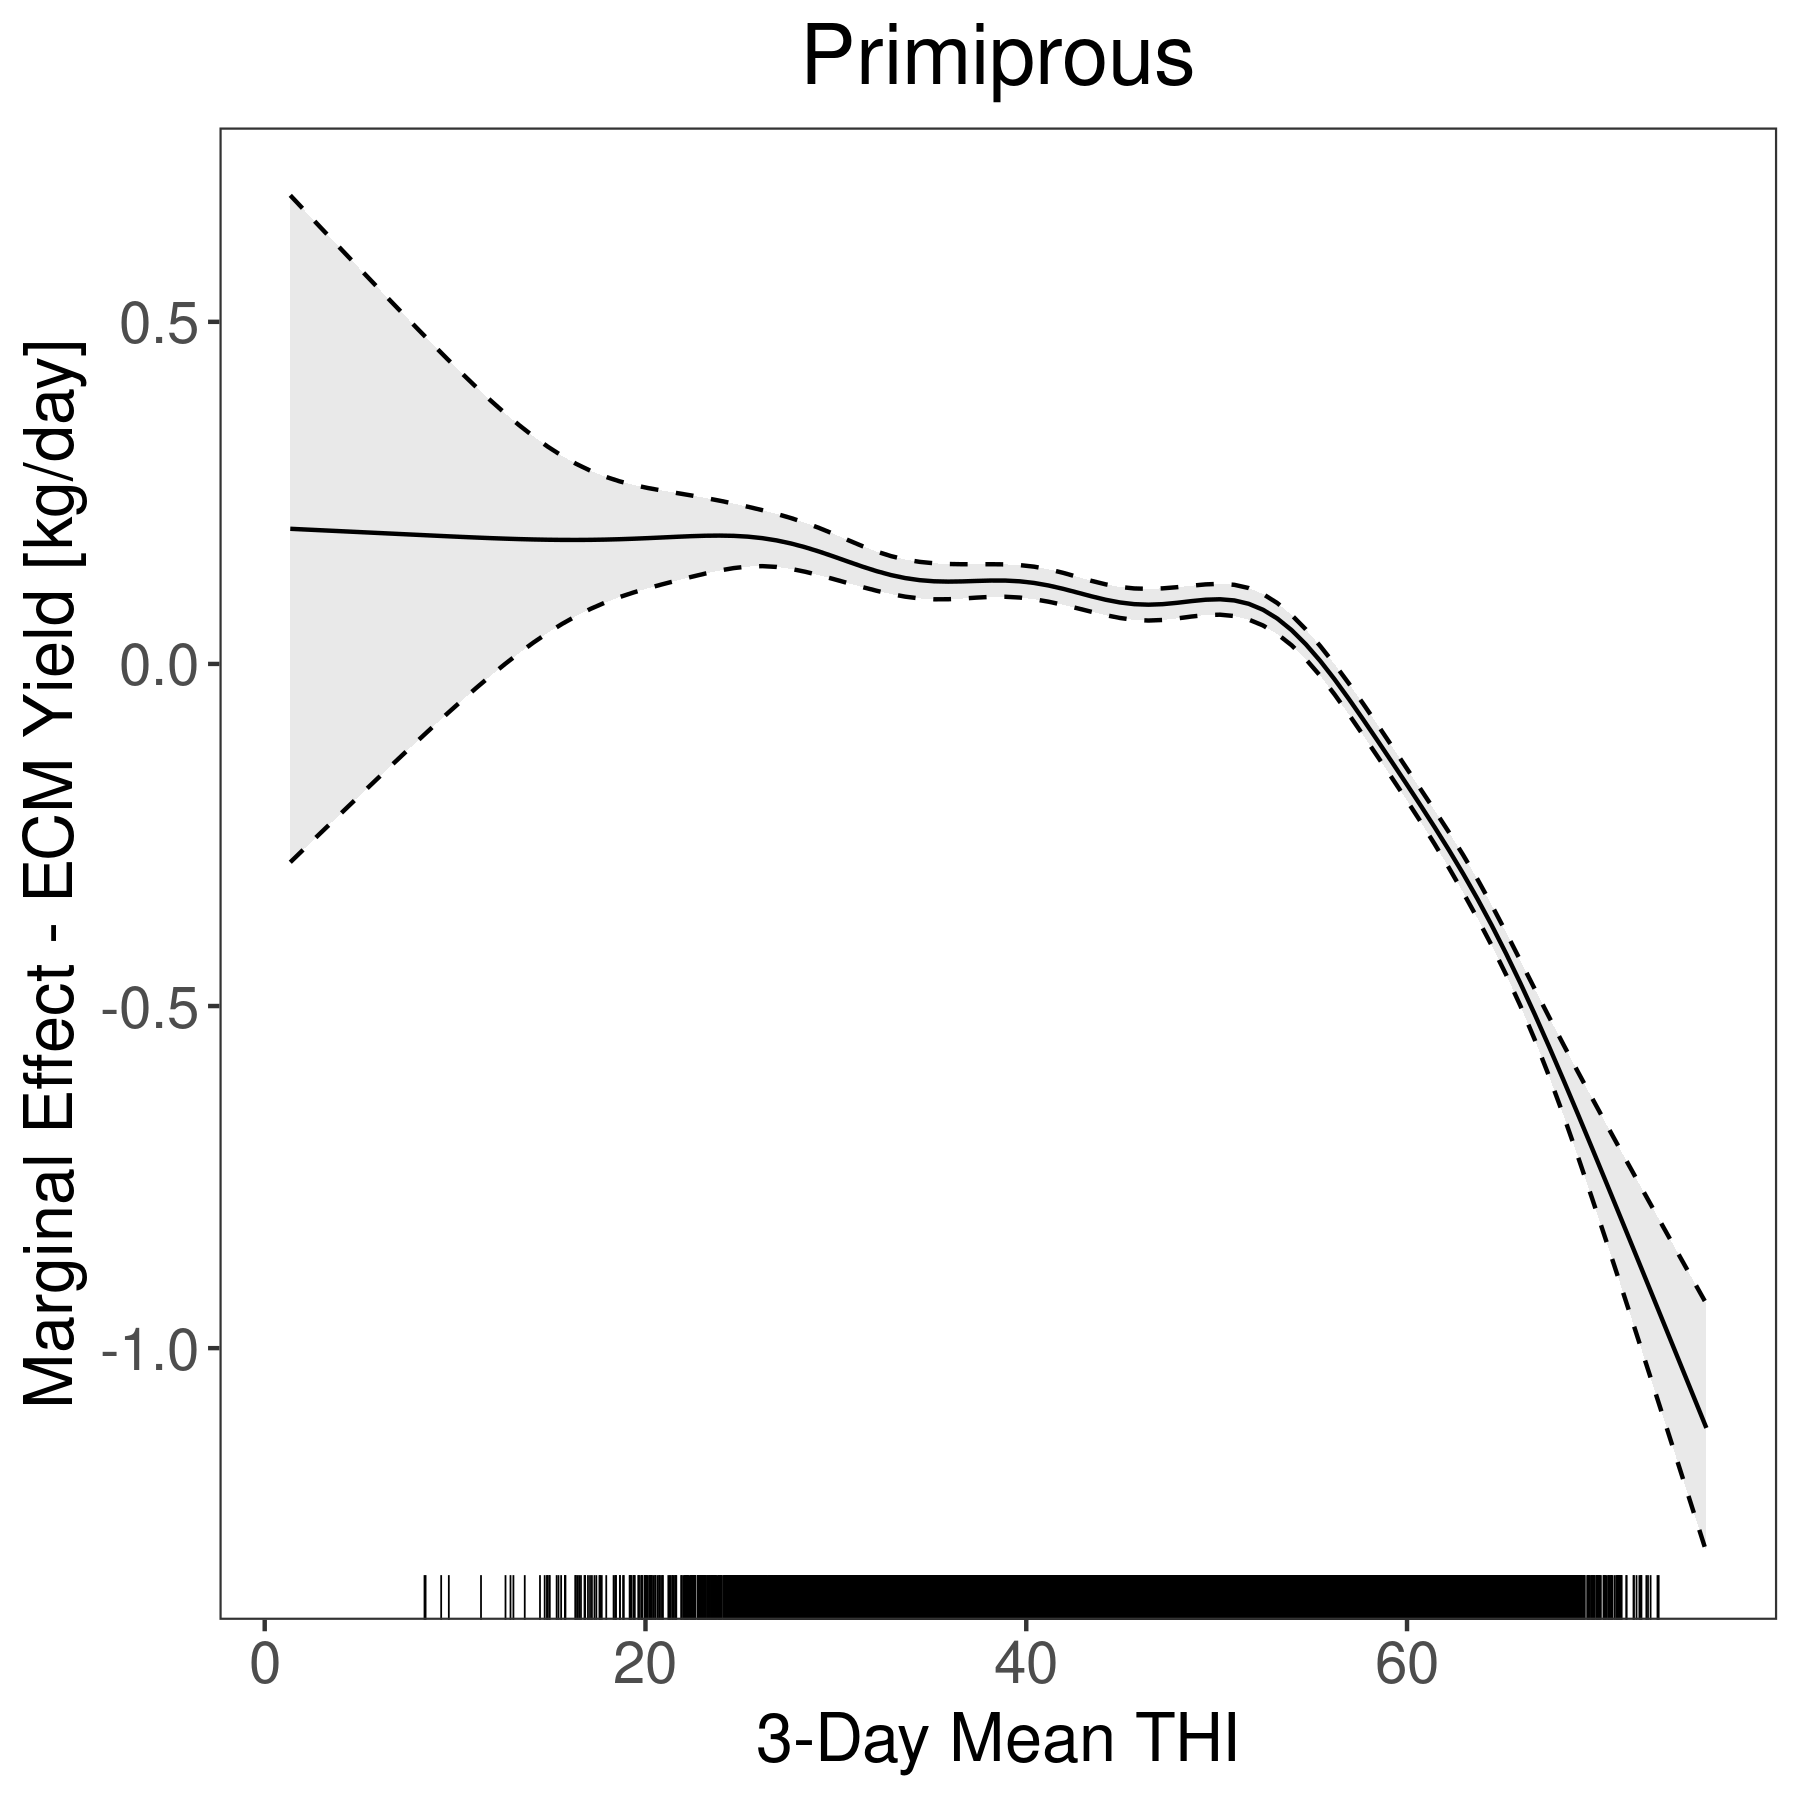
\includegraphics[width=\textwidth]{thesis/figures/models/ecm/before2010/sf_ecm_before2010/sf_ecm_before2010_marginal_thi_milk_primi.png}
    \end{subfigure}
    \hspace{0.05\textwidth} % Optional space between the figures
    \begin{subfigure}[b]{0.45\textwidth}
        \centering
        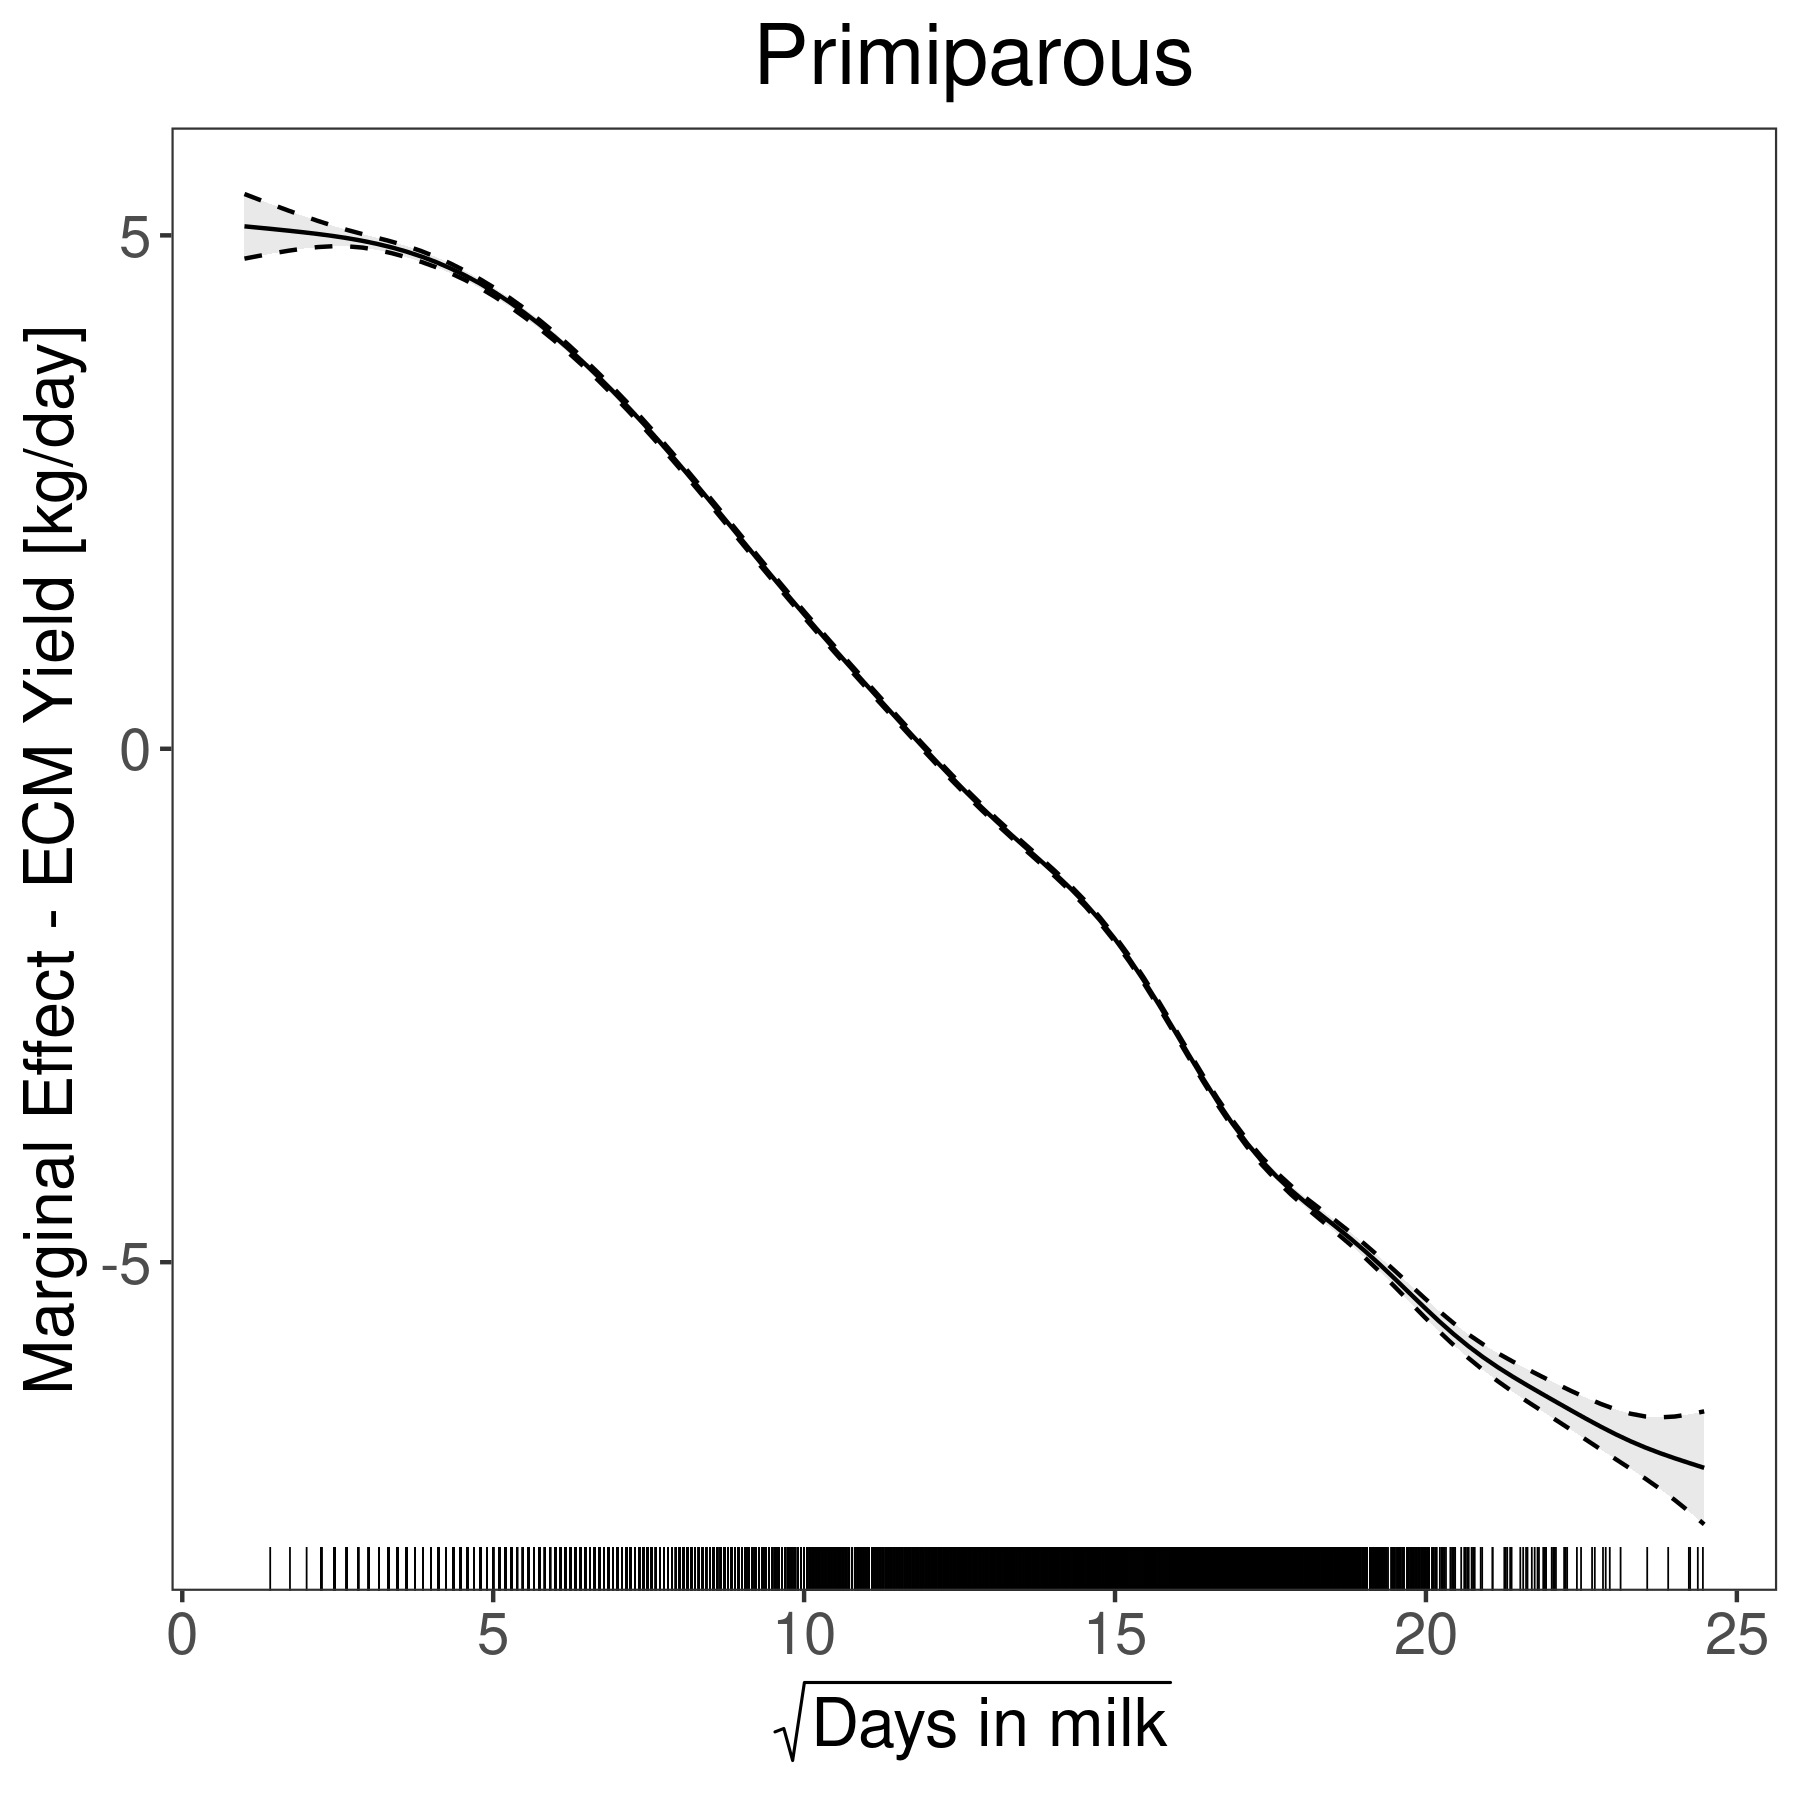
\includegraphics[width=\textwidth]{thesis/figures/models/ecm/before2010/sf_ecm_before2010/sf_ecm_before2010_marginal_dim_milk_primi.png}
    \end{subfigure}
    \begin{subfigure}[b]{0.45\textwidth}
        \centering
        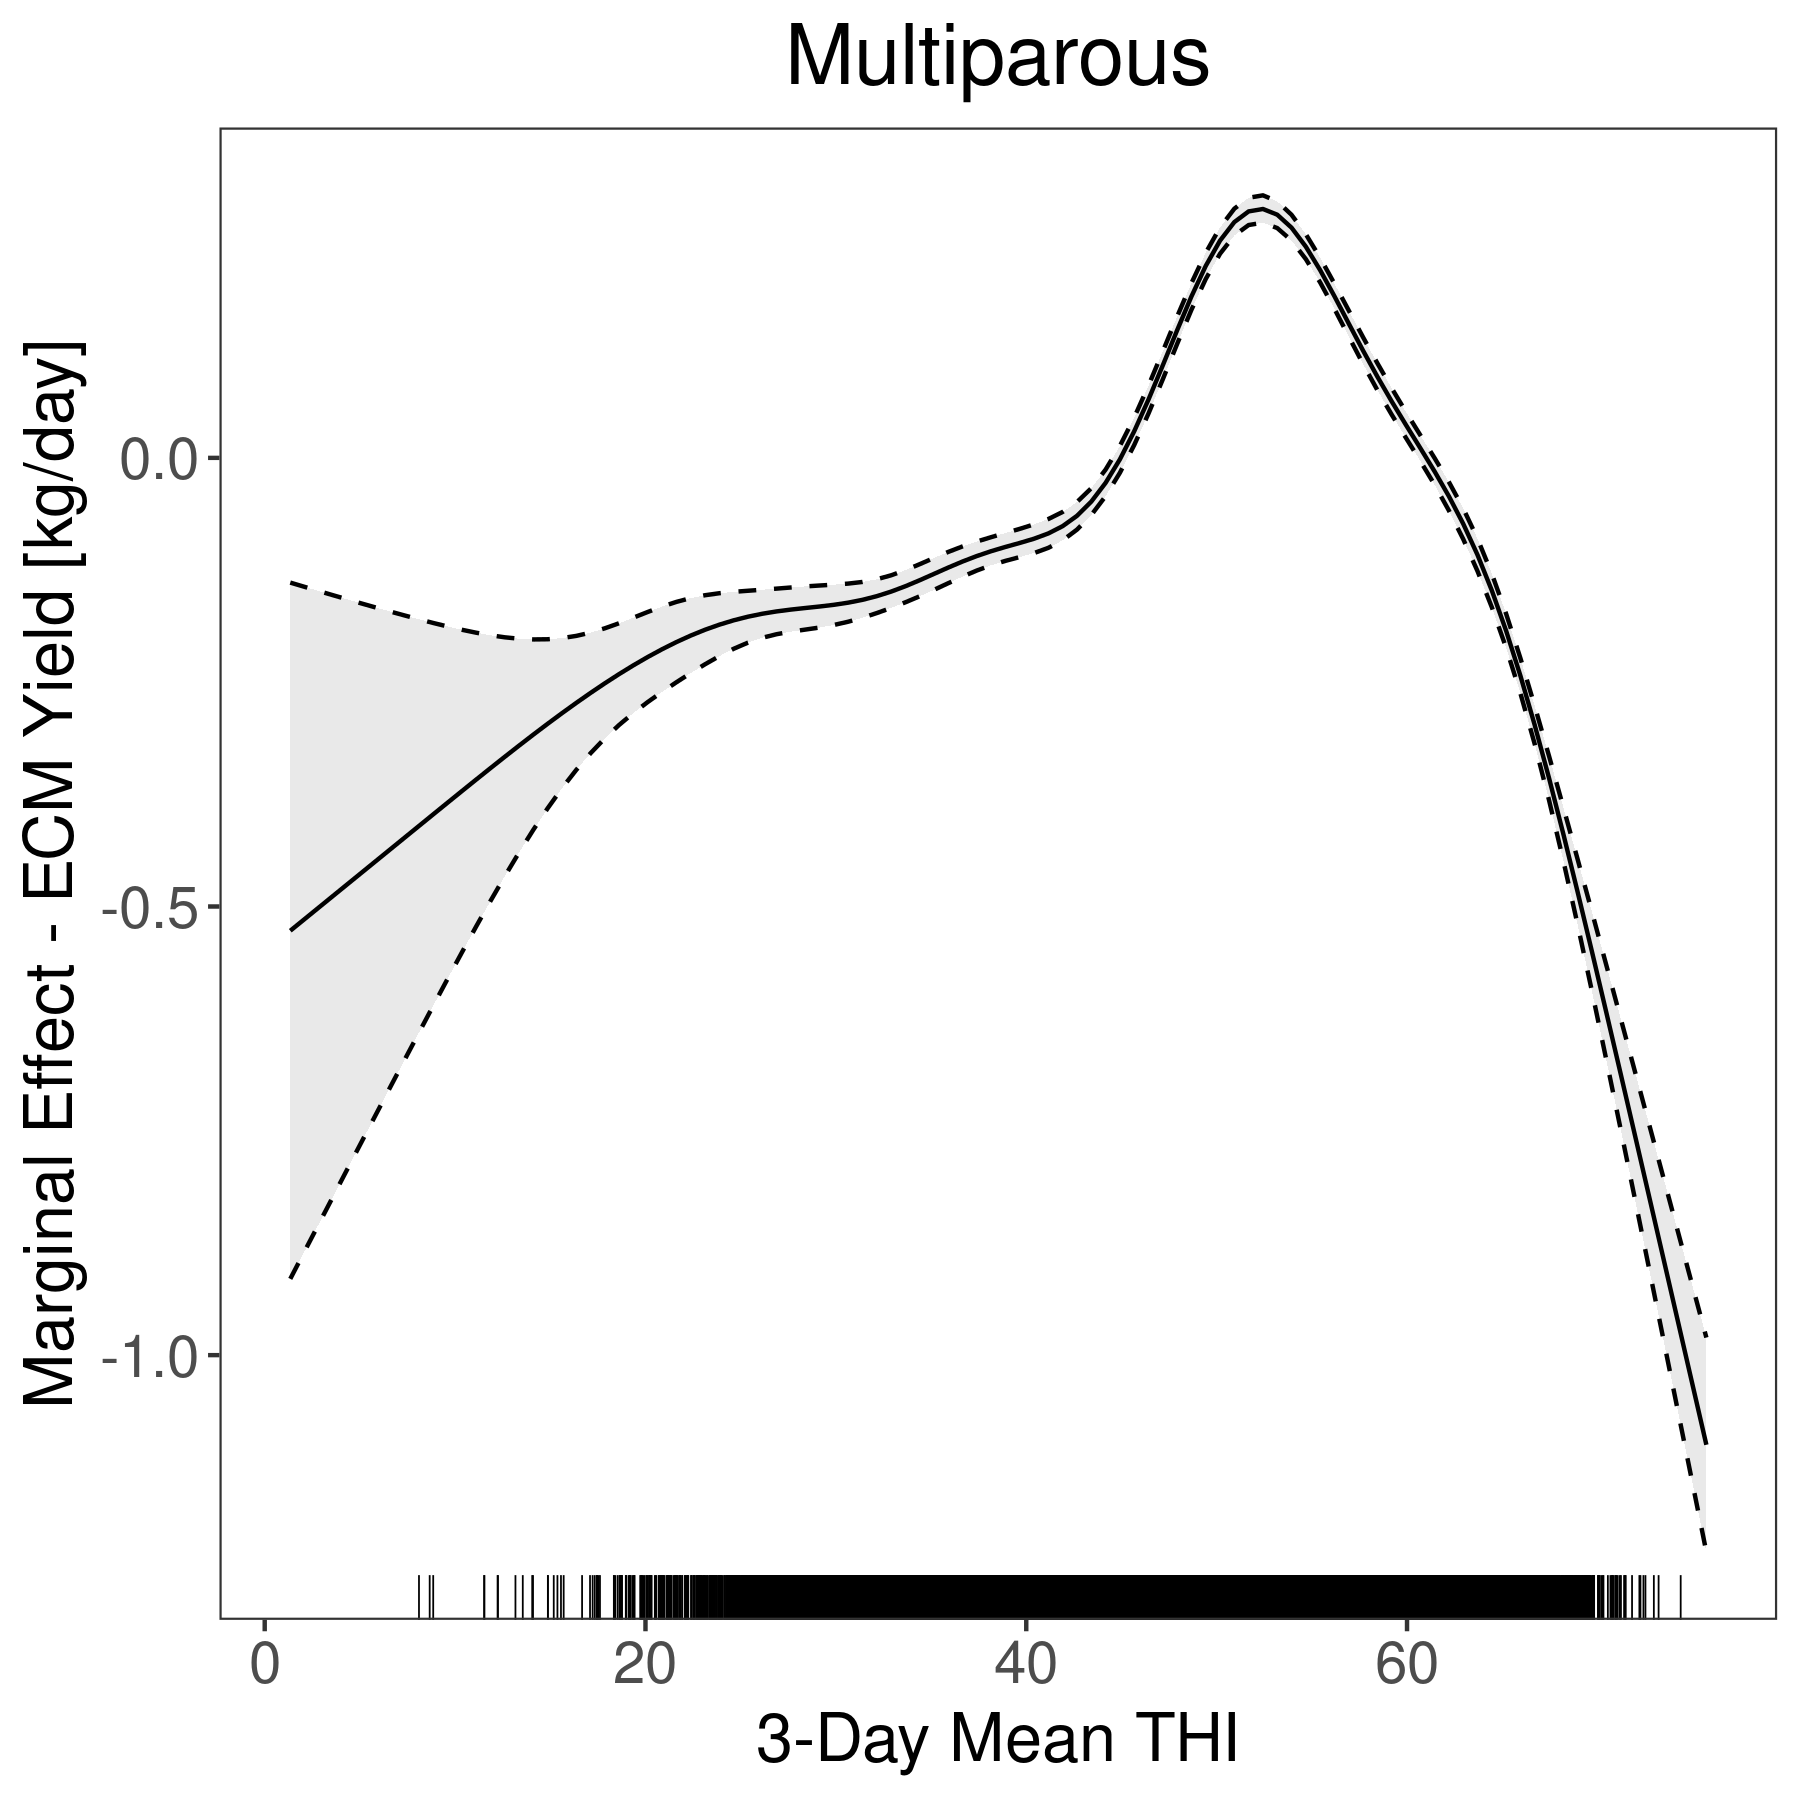
\includegraphics[width=\textwidth]{thesis/figures/models/ecm/before2010/sf_ecm_before2010/sf_ecm_before2010_marginal_thi_milk_multi.png}
    \end{subfigure}
    \hspace{0.05\textwidth} % Optional space between the figures
    \begin{subfigure}[b]{0.45\textwidth}
        \centering
        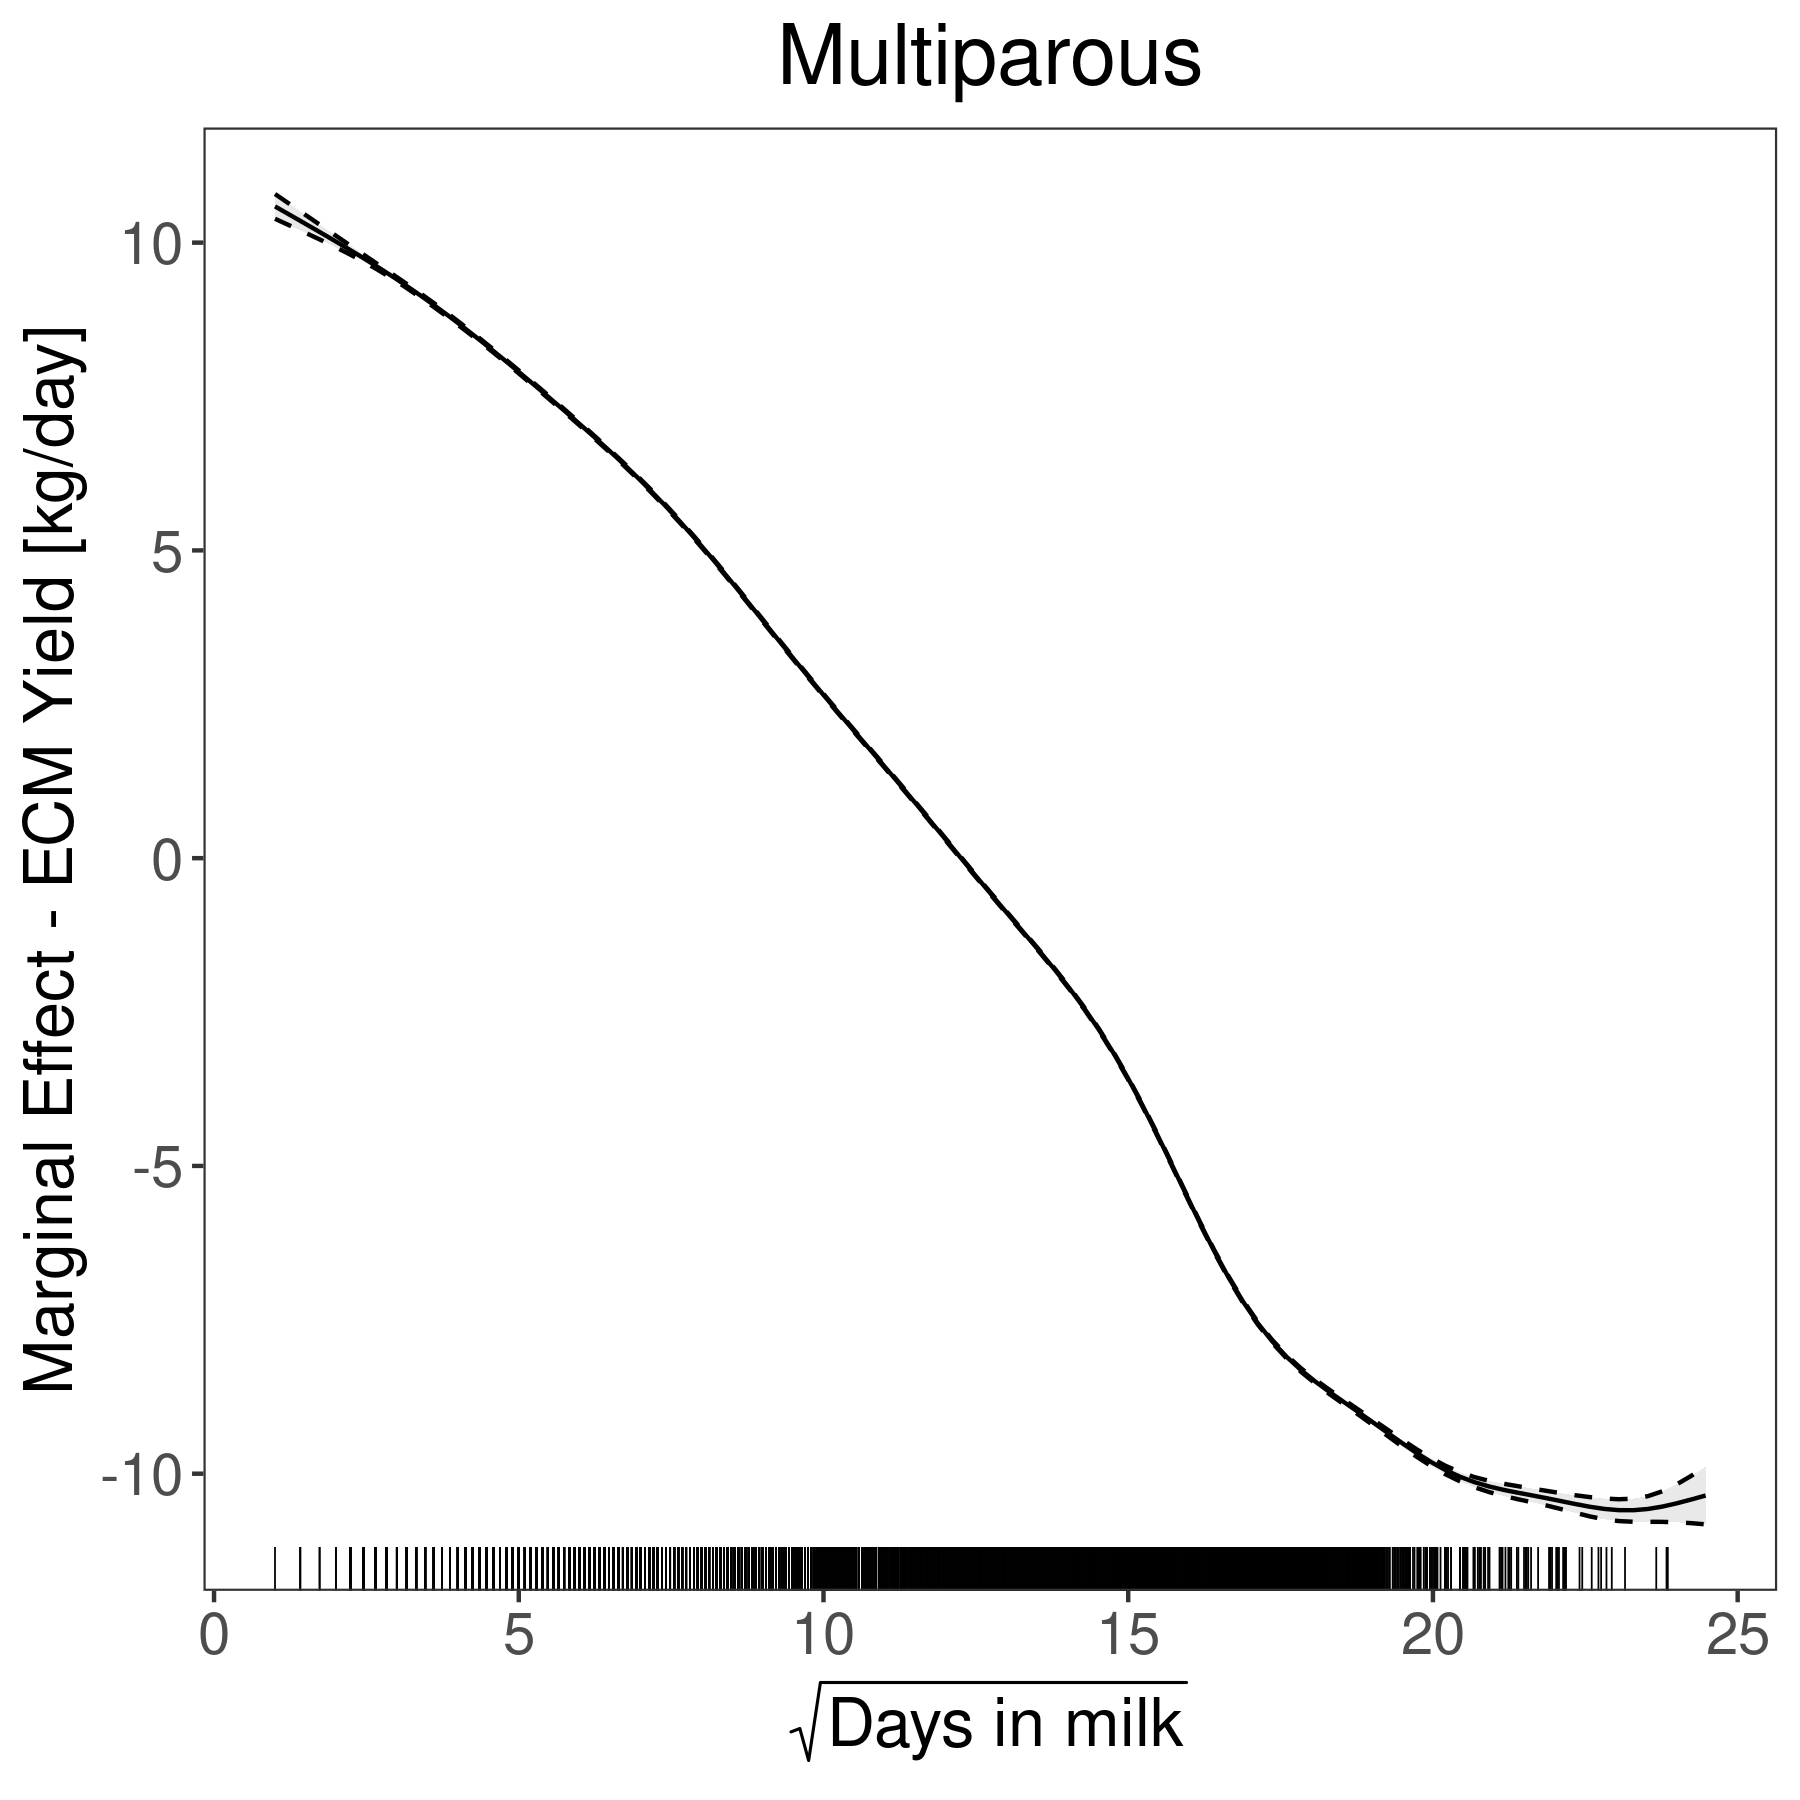
\includegraphics[width=\textwidth]{thesis/figures/models/ecm/before2010/sf_ecm_before2010/sf_ecm_before2010_marginal_dim_milk_multi.png}
    \end{subfigure}
    \caption[]{Swiss Fleckvieh: ECM Yield - 1984 - 2010 - THI Effect and Lactation Curve}
    \label{fig:main}
\end{figure}

\subsubsection{Split Period: 2010 - 2023}\label{model:sf_ecm_after}

\paragraph{Model Summary} \quad \\

    \begin{table}[H]
    \centering
    \begin{tabular}{lrrrr}
    \textbf{A. parametric coefficients} & Estimate & Std. Error & t-value & p-value \\ 
       \hline
       \hline
      (Intercept) & 23.9154 & 0.2931 & 81.5860 & $<$ 0.0001 \\ 
      parityprimiparous & -3.9004 & 0.0167 & -232.8837 & $<$ 0.0001 \\ 
      year2012 & -0.0690 & 0.3447 & -0.2002 & 0.8413 \\ 
      year2013 & -0.3623 & 0.3299 & -1.0981 & 0.2722 \\ 
      year2014 & 0.1886 & 0.3276 & 0.5756 & 0.5649 \\ 
      year2015 & 0.5104 & 0.3329 & 1.5333 & 0.1252 \\ 
      year2016 & 0.9654 & 0.3357 & 2.8755 & 0.0040 \\ 
      year2017 & 1.2575 & 0.3307 & 3.8024 & 0.0001 \\ 
      year2018 & 1.7924 & 0.3342 & 5.3623 & $<$ 0.0001 \\ 
      year2019 & 1.9137 & 0.3315 & 5.7726 & $<$ 0.0001 \\ 
      year2020 & 2.3420 & 0.3412 & 6.8648 & $<$ 0.0001 \\ 
      year2021 & 2.6223 & 0.3210 & 8.1692 & $<$ 0.0001 \\ 
      year2022 & 2.3548 & 0.3389 & 6.9490 & $<$ 0.0001 \\ 
      year2023 & 2.6795 & 0.3323 & 8.0634 & $<$ 0.0001 \\ 
       \hline
    \textbf{B. smooth terms} & edf & Ref.df & F-value & p-value \\ 
    \hline
    \hline
      s(thi\_mean\_t0\_3d):paritymultiparous & 7.9356 & 7.9356 & 208.7322 & $<$ 0.0001 \\ 
      s(thi\_mean\_t0\_3d):parityprimiparous & 6.5668 & 6.5668 & 165.3686 & $<$ 0.0001 \\ 
      s(days\_in\_milk\_t):paritymultiparous & 13.4184 & 13.4184 & 85993.6942 & $<$ 0.0001 \\ 
      s(days\_in\_milk\_t):parityprimiparous & 12.3905 & 12.3905 & 6667.4461 & $<$ 0.0001 \\ 
       \hline
    \end{tabular}
    \caption[]{Swiss Fleckvieh: ECM Yield - 2011-2023 - GAMM model summary without random effect terms.}
    \end{table}

\newpage
\begin{table}[H]
\centering
\begin{tabular}
{l | r | r | r | r}
\textbf{Smooth Term Fixed Effect} & Est. & SE & z & p\\
\hline
\hline
s(thi\_mean\_t0\_3d):multiFx1 & -0.0875 & 0.0974 & -0.90 & 0.3691\\
s(thi\_mean\_t0\_3d):primiFx1 & -0.5661 & 0.1180 & -4.80 & $<$ 1e-05\\
s(days\_in\_milk\_):multiFx1 & -0.3719 & 0.4377 & -0.85 & 0.3955\\
s(days\_in\_milk\_):primiFx1 & 1.7240 & 0.5478 & 3.15 & 0.0017\\
\hline
\textbf{Variance Component} & Estimated $\sigma$ & & & \\
\hline
\hline
$\sigma_\alpha$ & 2.7517 & & & \\
$\sigma_\iota$ & 1.1372 & & & \\
$\sigma_\phi$ & 3.7572 & & & \\
s(thi\_mean\_t0\_3d):multi & 1.7293 & & & \\
s(days\_in\_milk\_):primi & 5.4432 & & & \\
s(days\_in\_milk\_):multi & 7.1565 & & & \\
s(thi\_mean\_t0\_3d):primi & 1.4283 & & & \\
Residual & 3.9215 & & & \\
\end{tabular}
\caption[]{Swiss Fleckvieh: ECM Yield - 2011-2023 - Mixed Model Summary - Smooth Terms and Random Effects.}
\end{table}


\paragraph{Model Diagnostics} \quad \\
\begin{figure}[H]
    \centering
    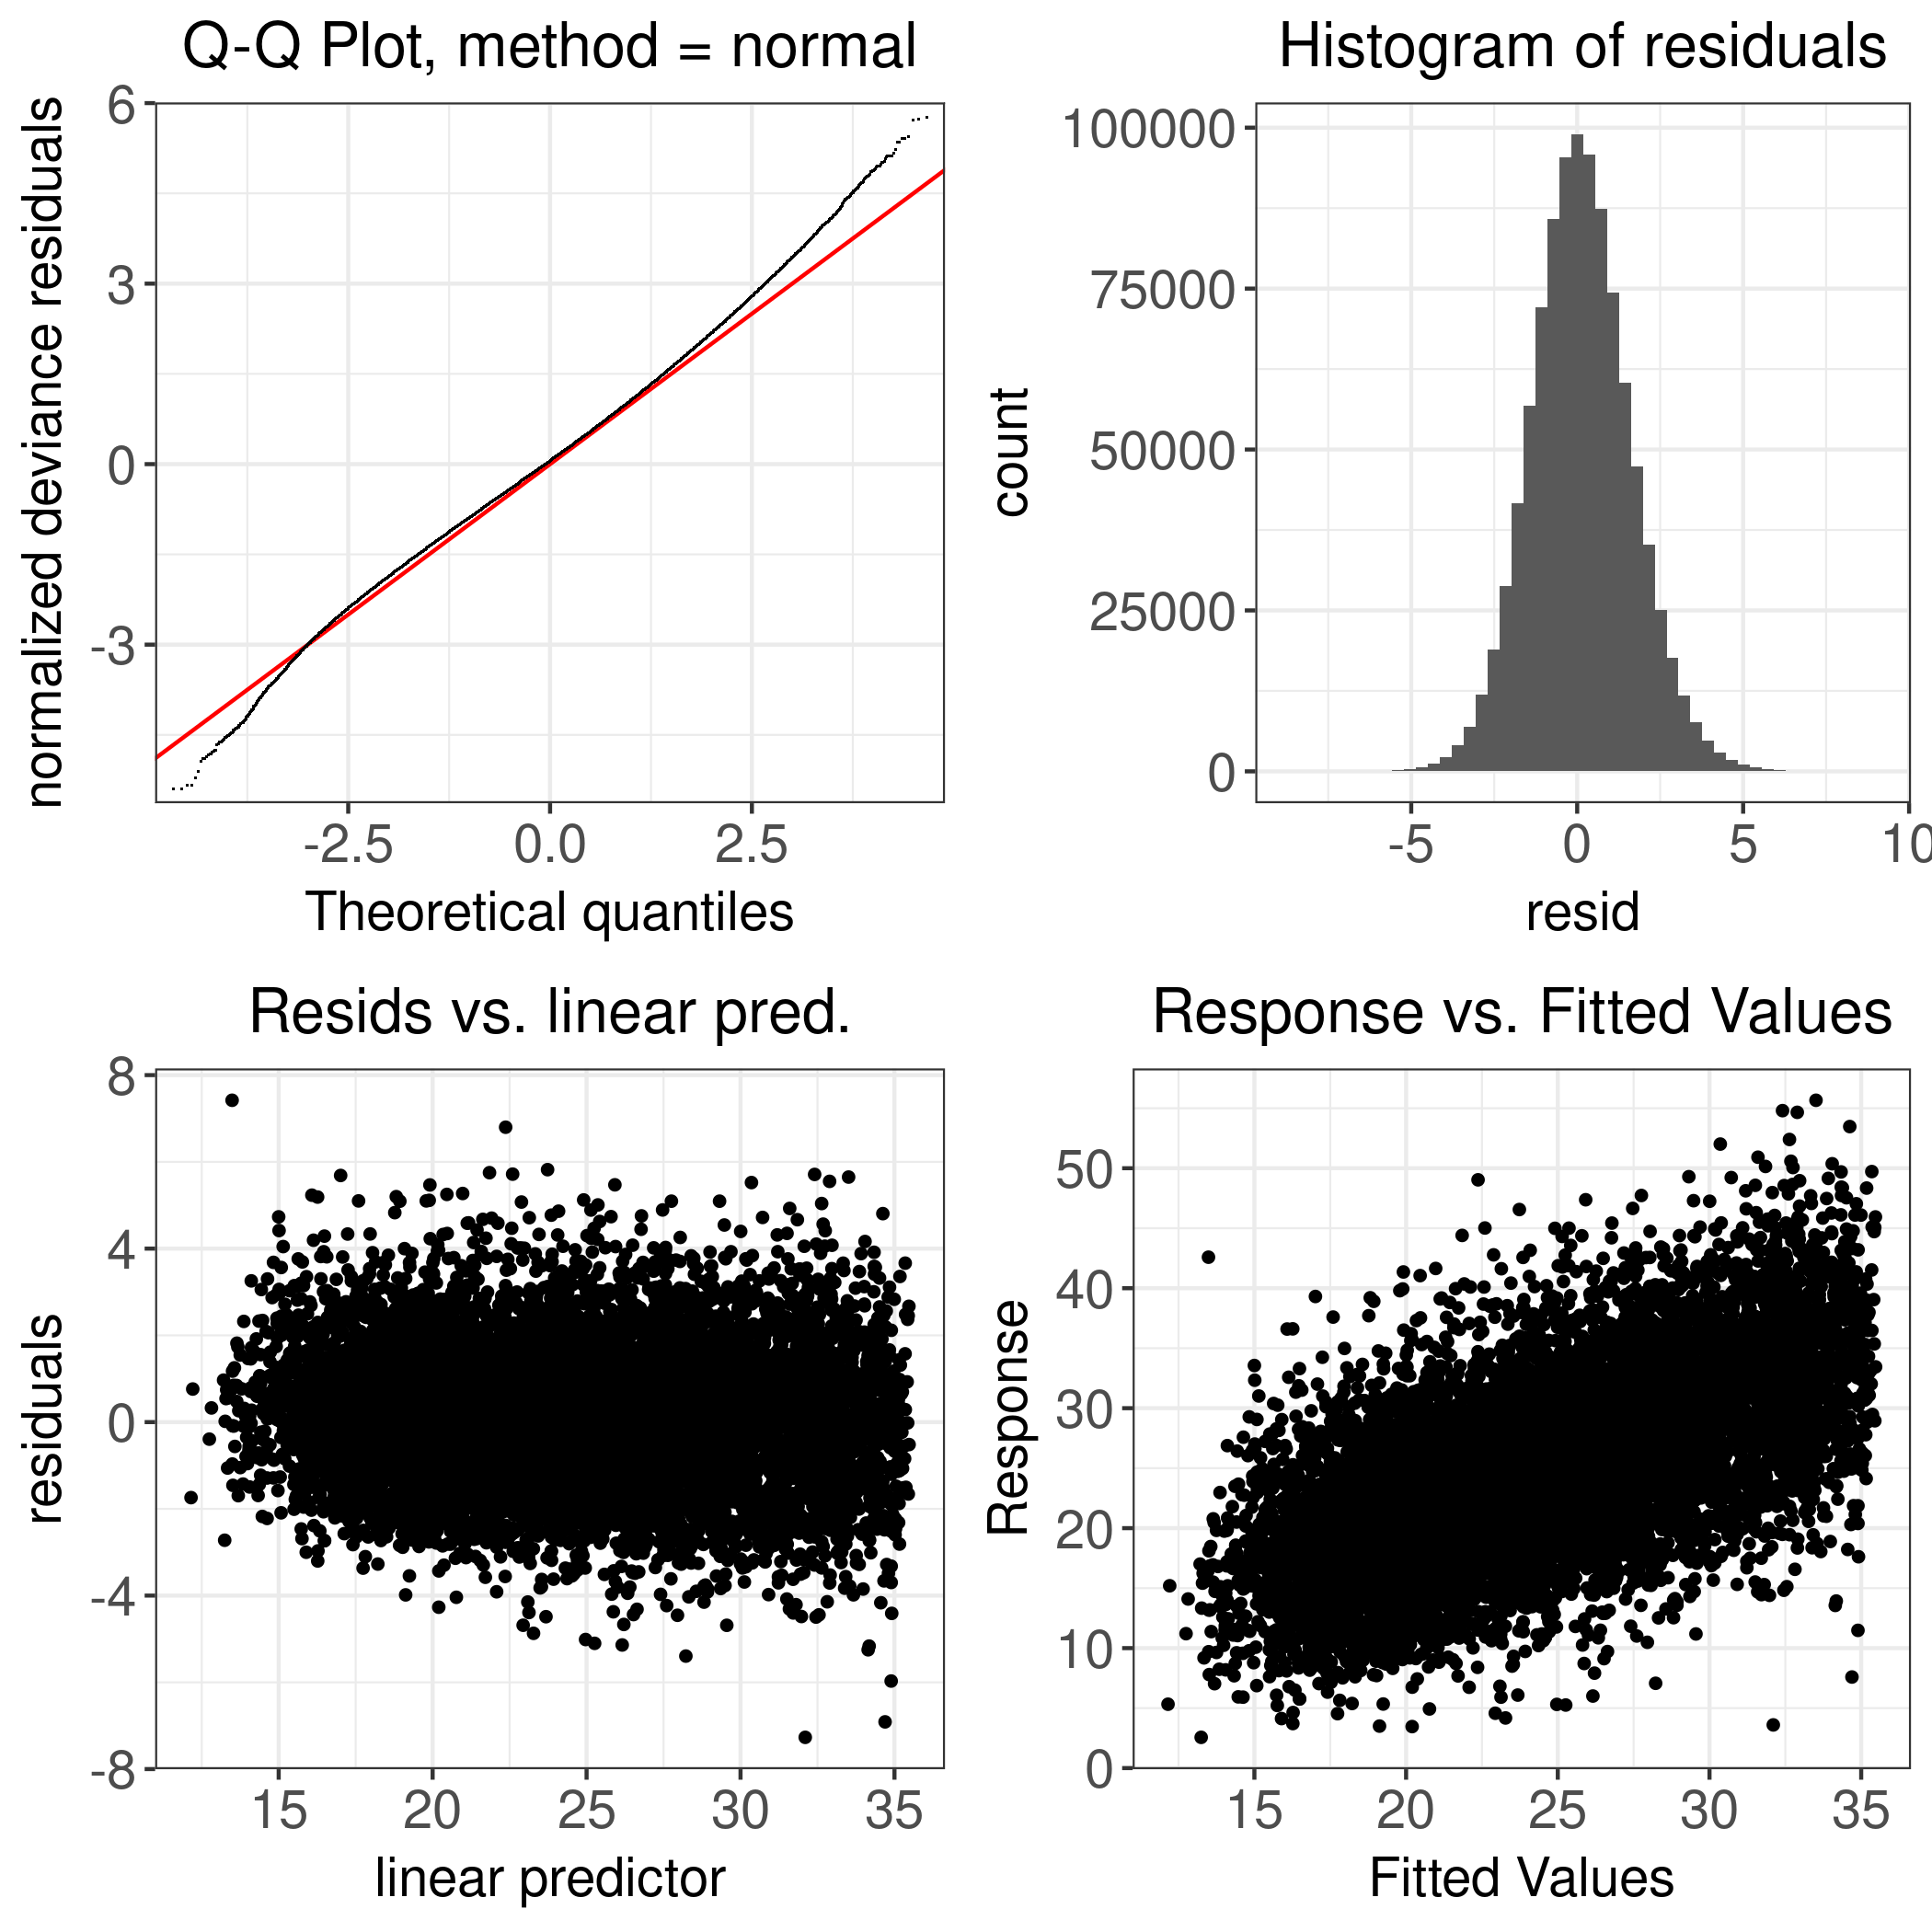
\includegraphics[width=0.6\textwidth]{thesis/figures/models/ecm/after2010/sf_ecm_after2010/sf_ecm_after2010_diagnostics.png}
    \caption[]{Swiss Fleckvieh: ECM Yield - 2011 - 2023 - Diagnostic Plot}
\end{figure}

\newpage
\paragraph{THI Effect and Lactation Curve} \quad \\
\begin{figure}[H]
    \centering
    \begin{subfigure}[b]{0.45\textwidth}
        \centering
        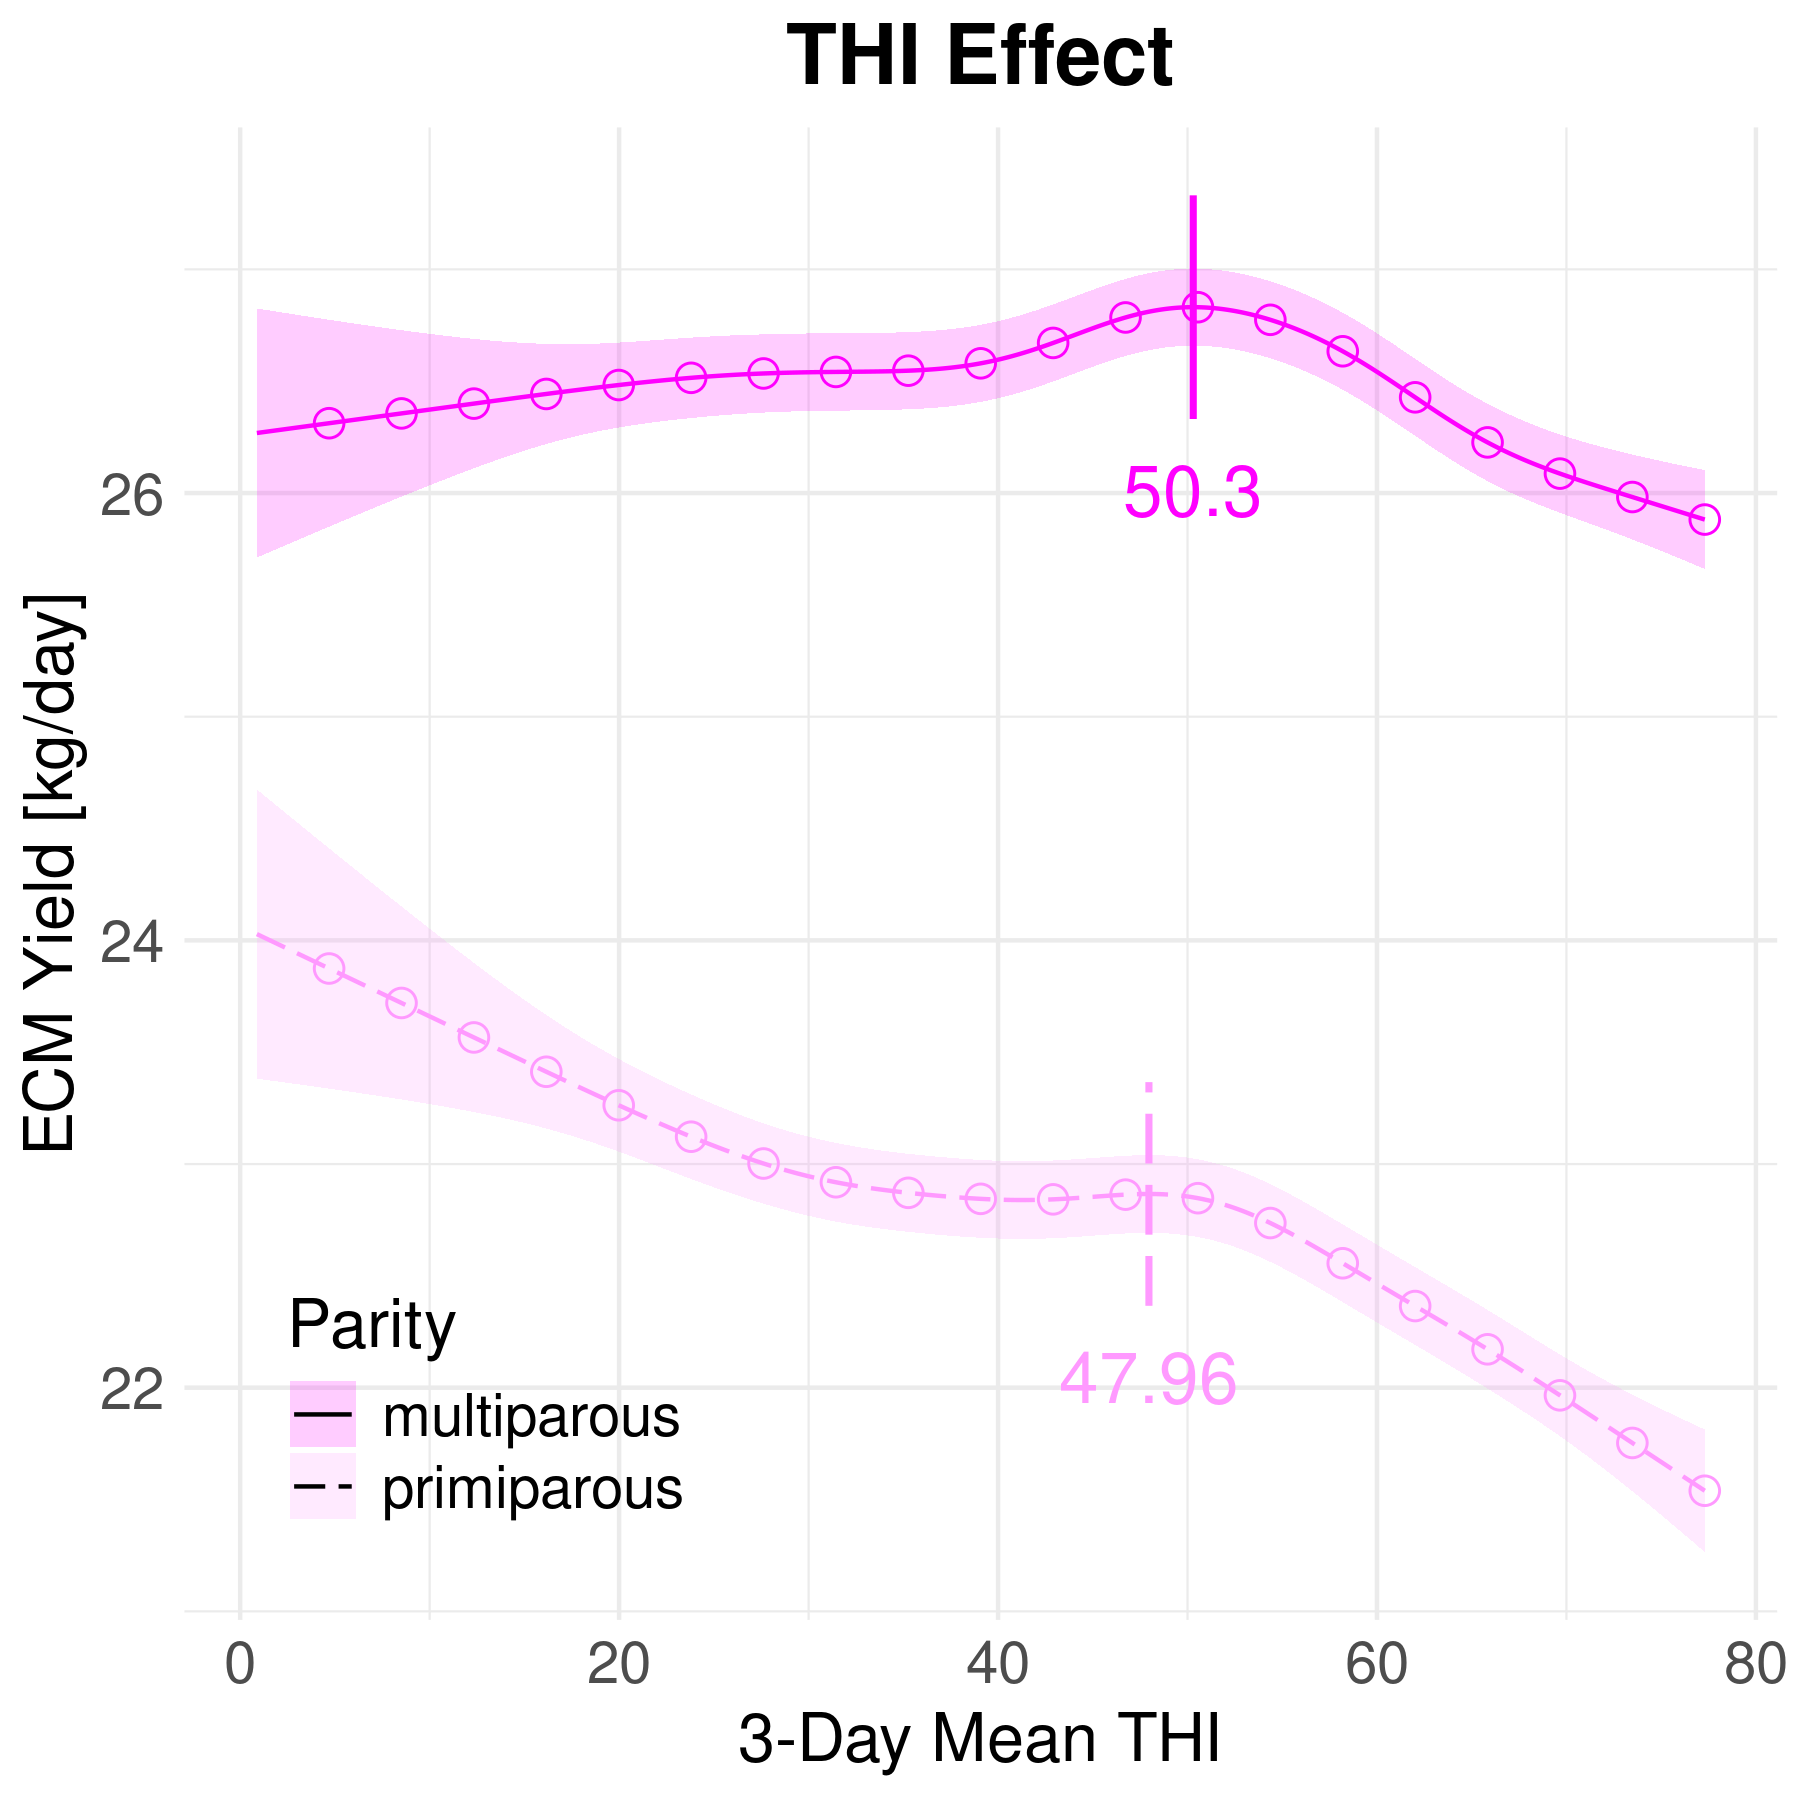
\includegraphics[width=\textwidth]{thesis/figures/models/ecm/after2010/sf_ecm_after2010/sf_ecm_after2010_marginal_thi_milk_combined.png}
    \end{subfigure}
    \hspace{0.05\textwidth} % Optional space between the figures
    \begin{subfigure}[b]{0.45\textwidth}
        \centering
        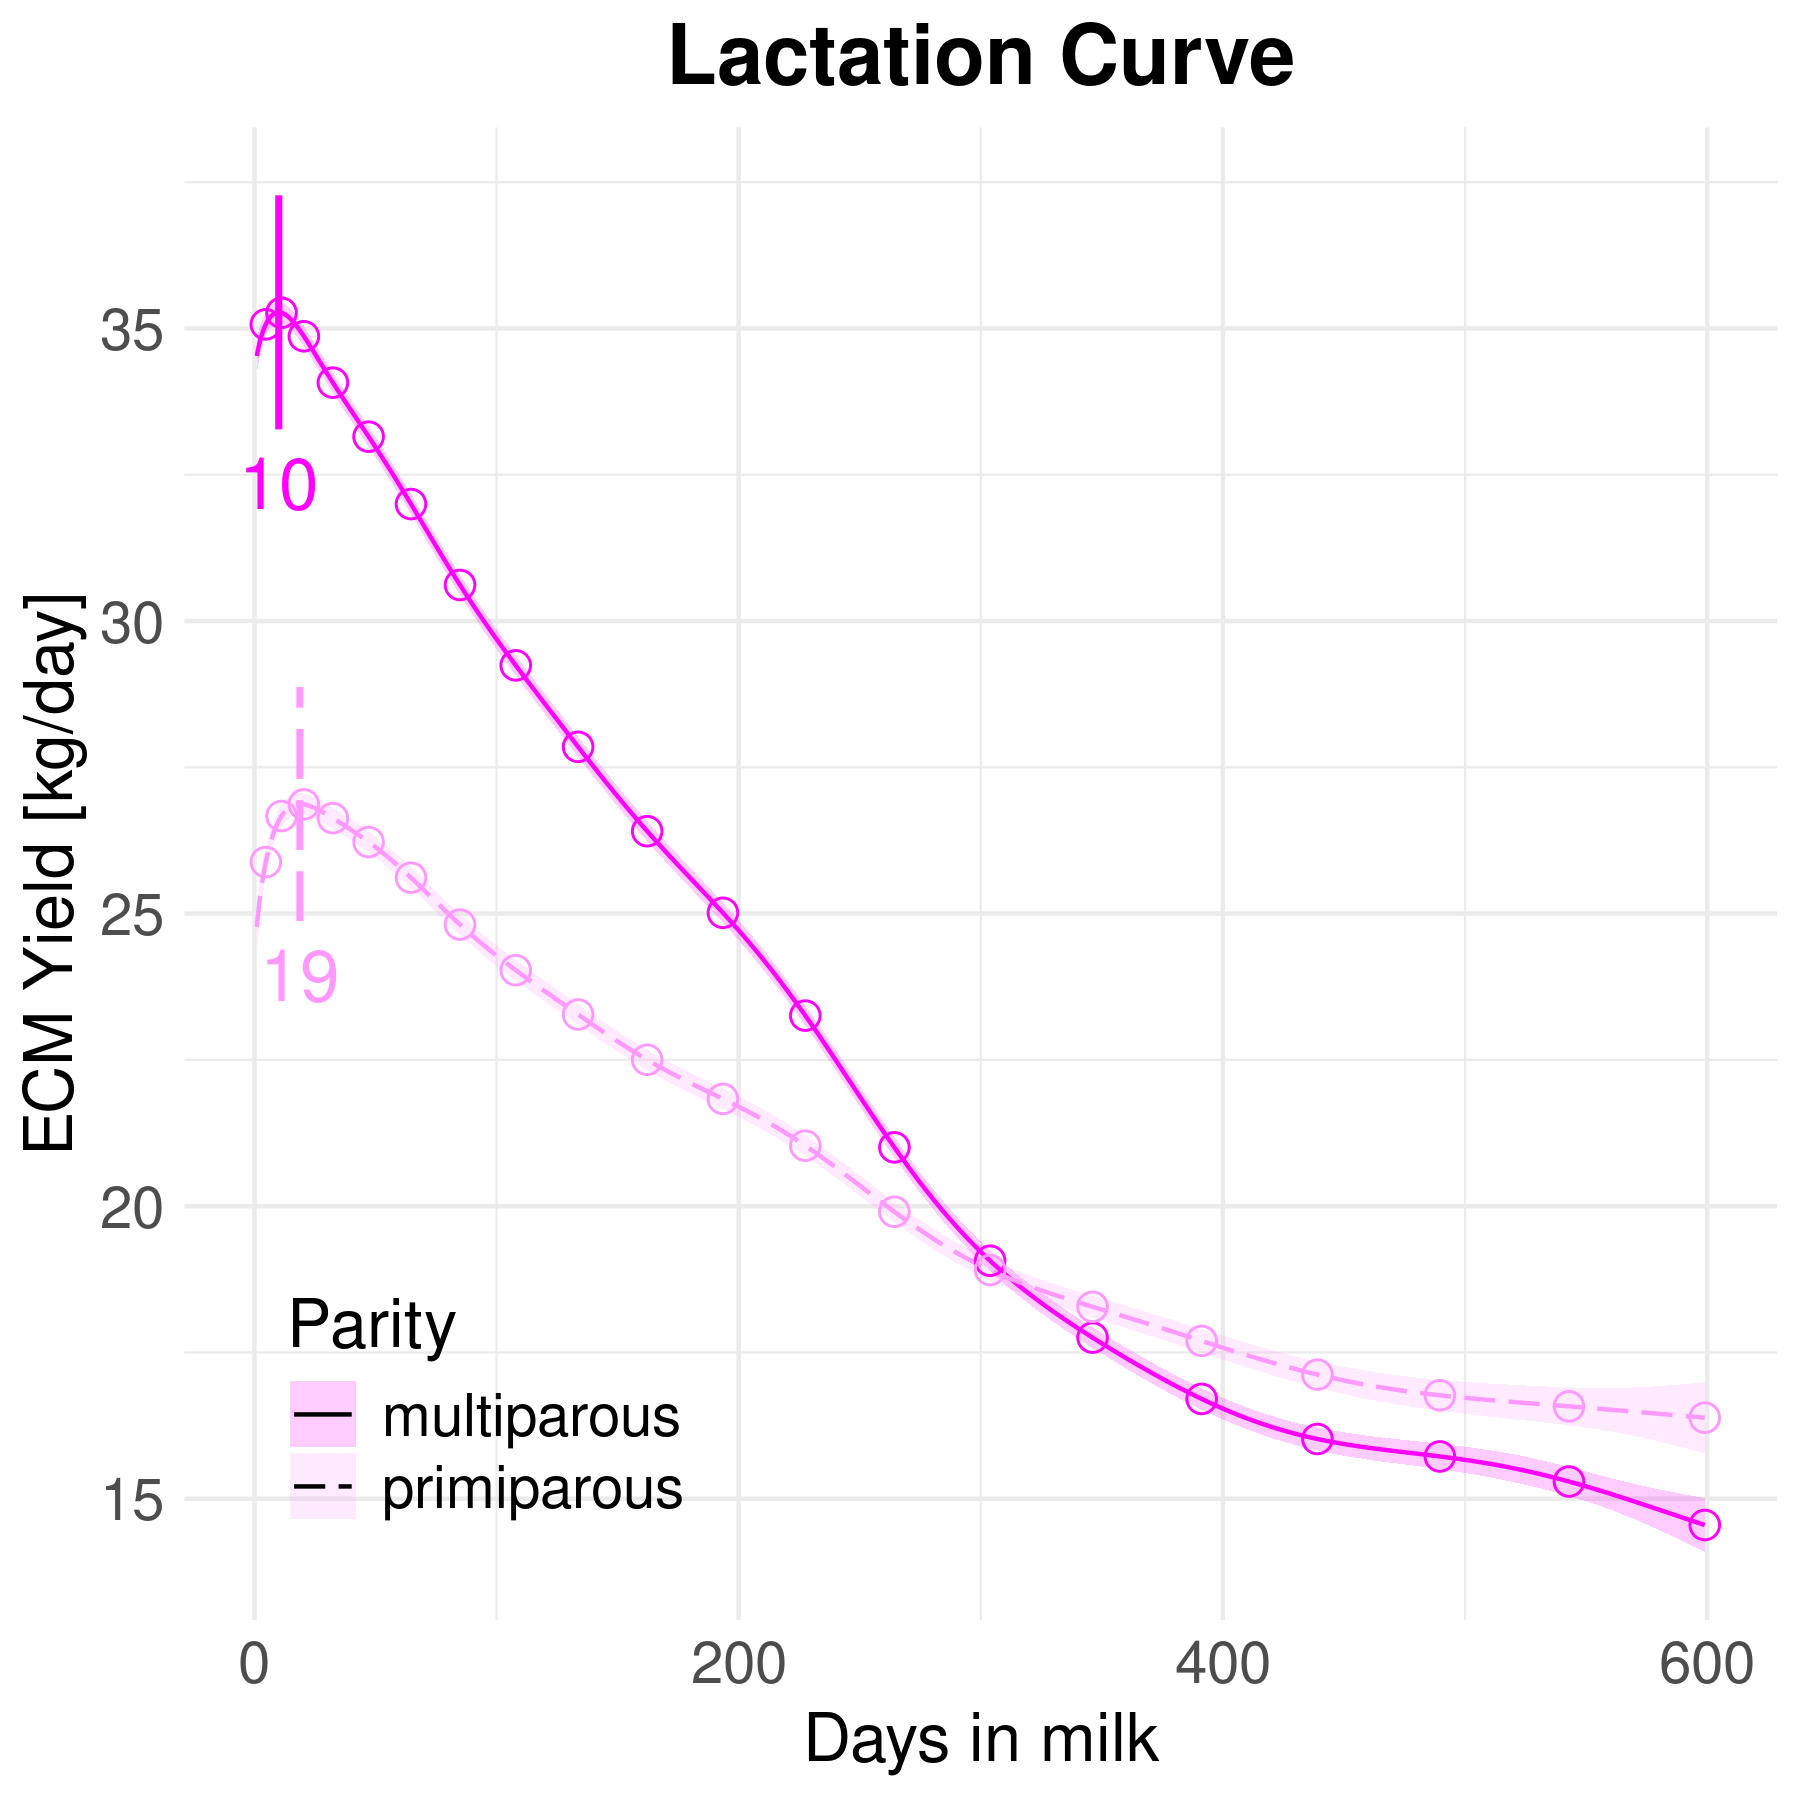
\includegraphics[width=\textwidth]{thesis/figures/models/ecm/after2010/sf_ecm_after2010/sf_ecm_after2010_marginal_dim_milk_combined.png}
    \end{subfigure}
    \begin{subfigure}[b]{0.45\textwidth}
        \centering
        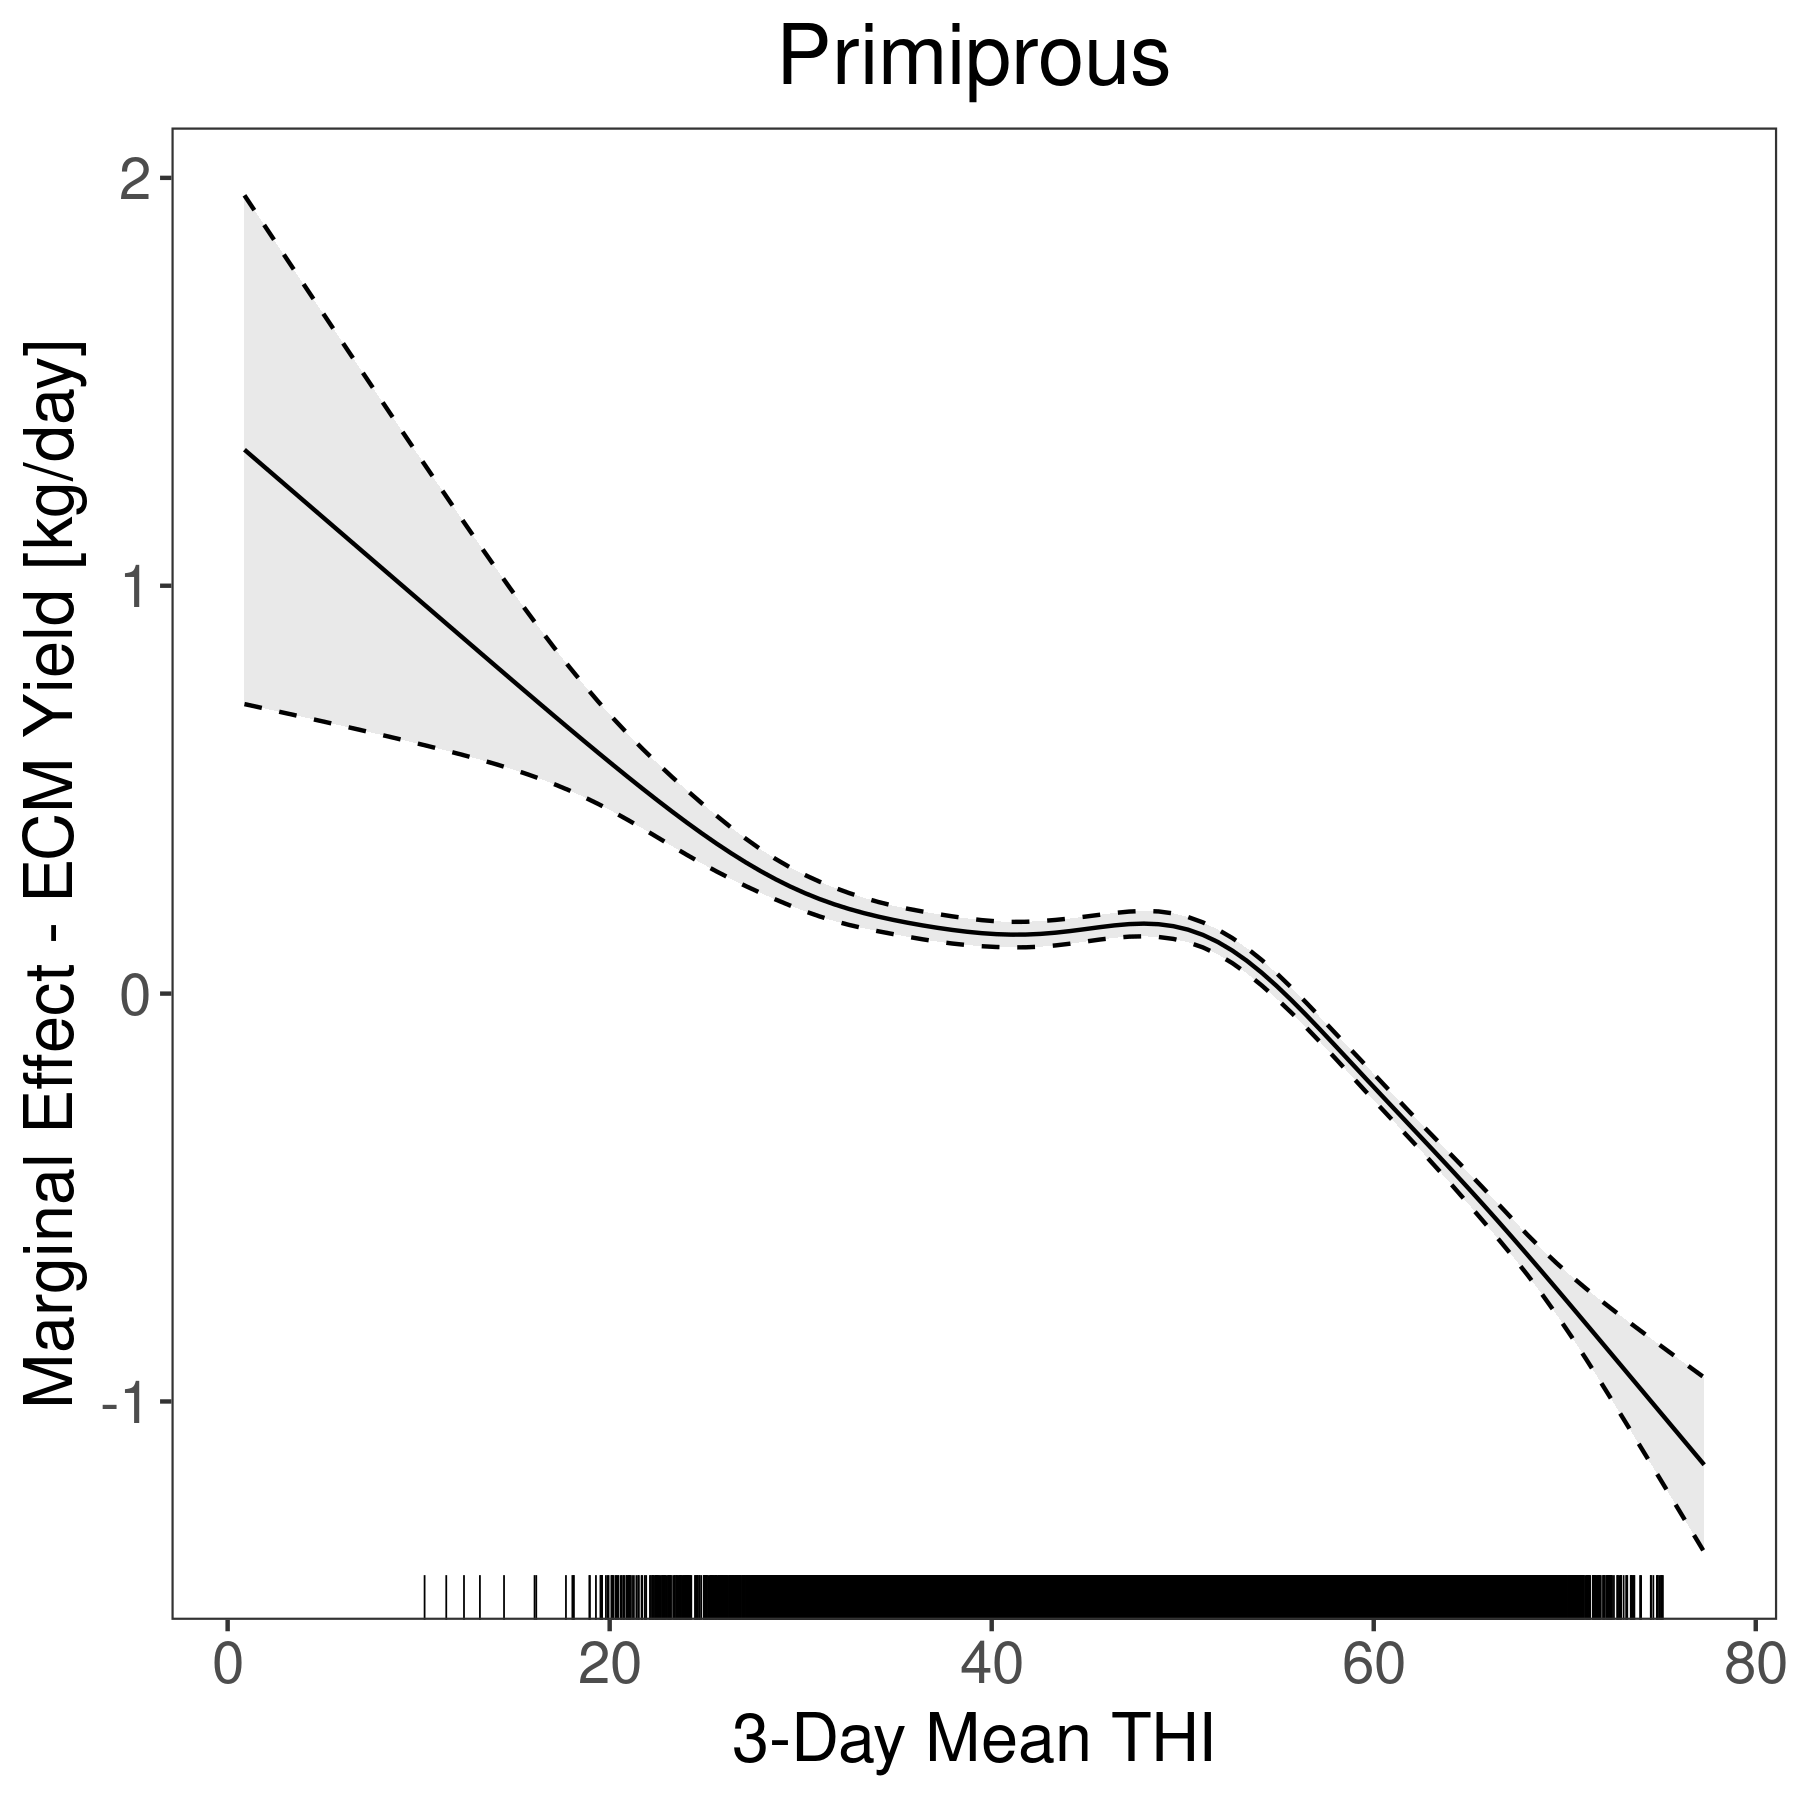
\includegraphics[width=\textwidth]{thesis/figures/models/ecm/after2010/sf_ecm_after2010/sf_ecm_after2010_marginal_thi_milk_primi.png}
    \end{subfigure}
    \hspace{0.05\textwidth} % Optional space between the figures
    \begin{subfigure}[b]{0.45\textwidth}
        \centering
        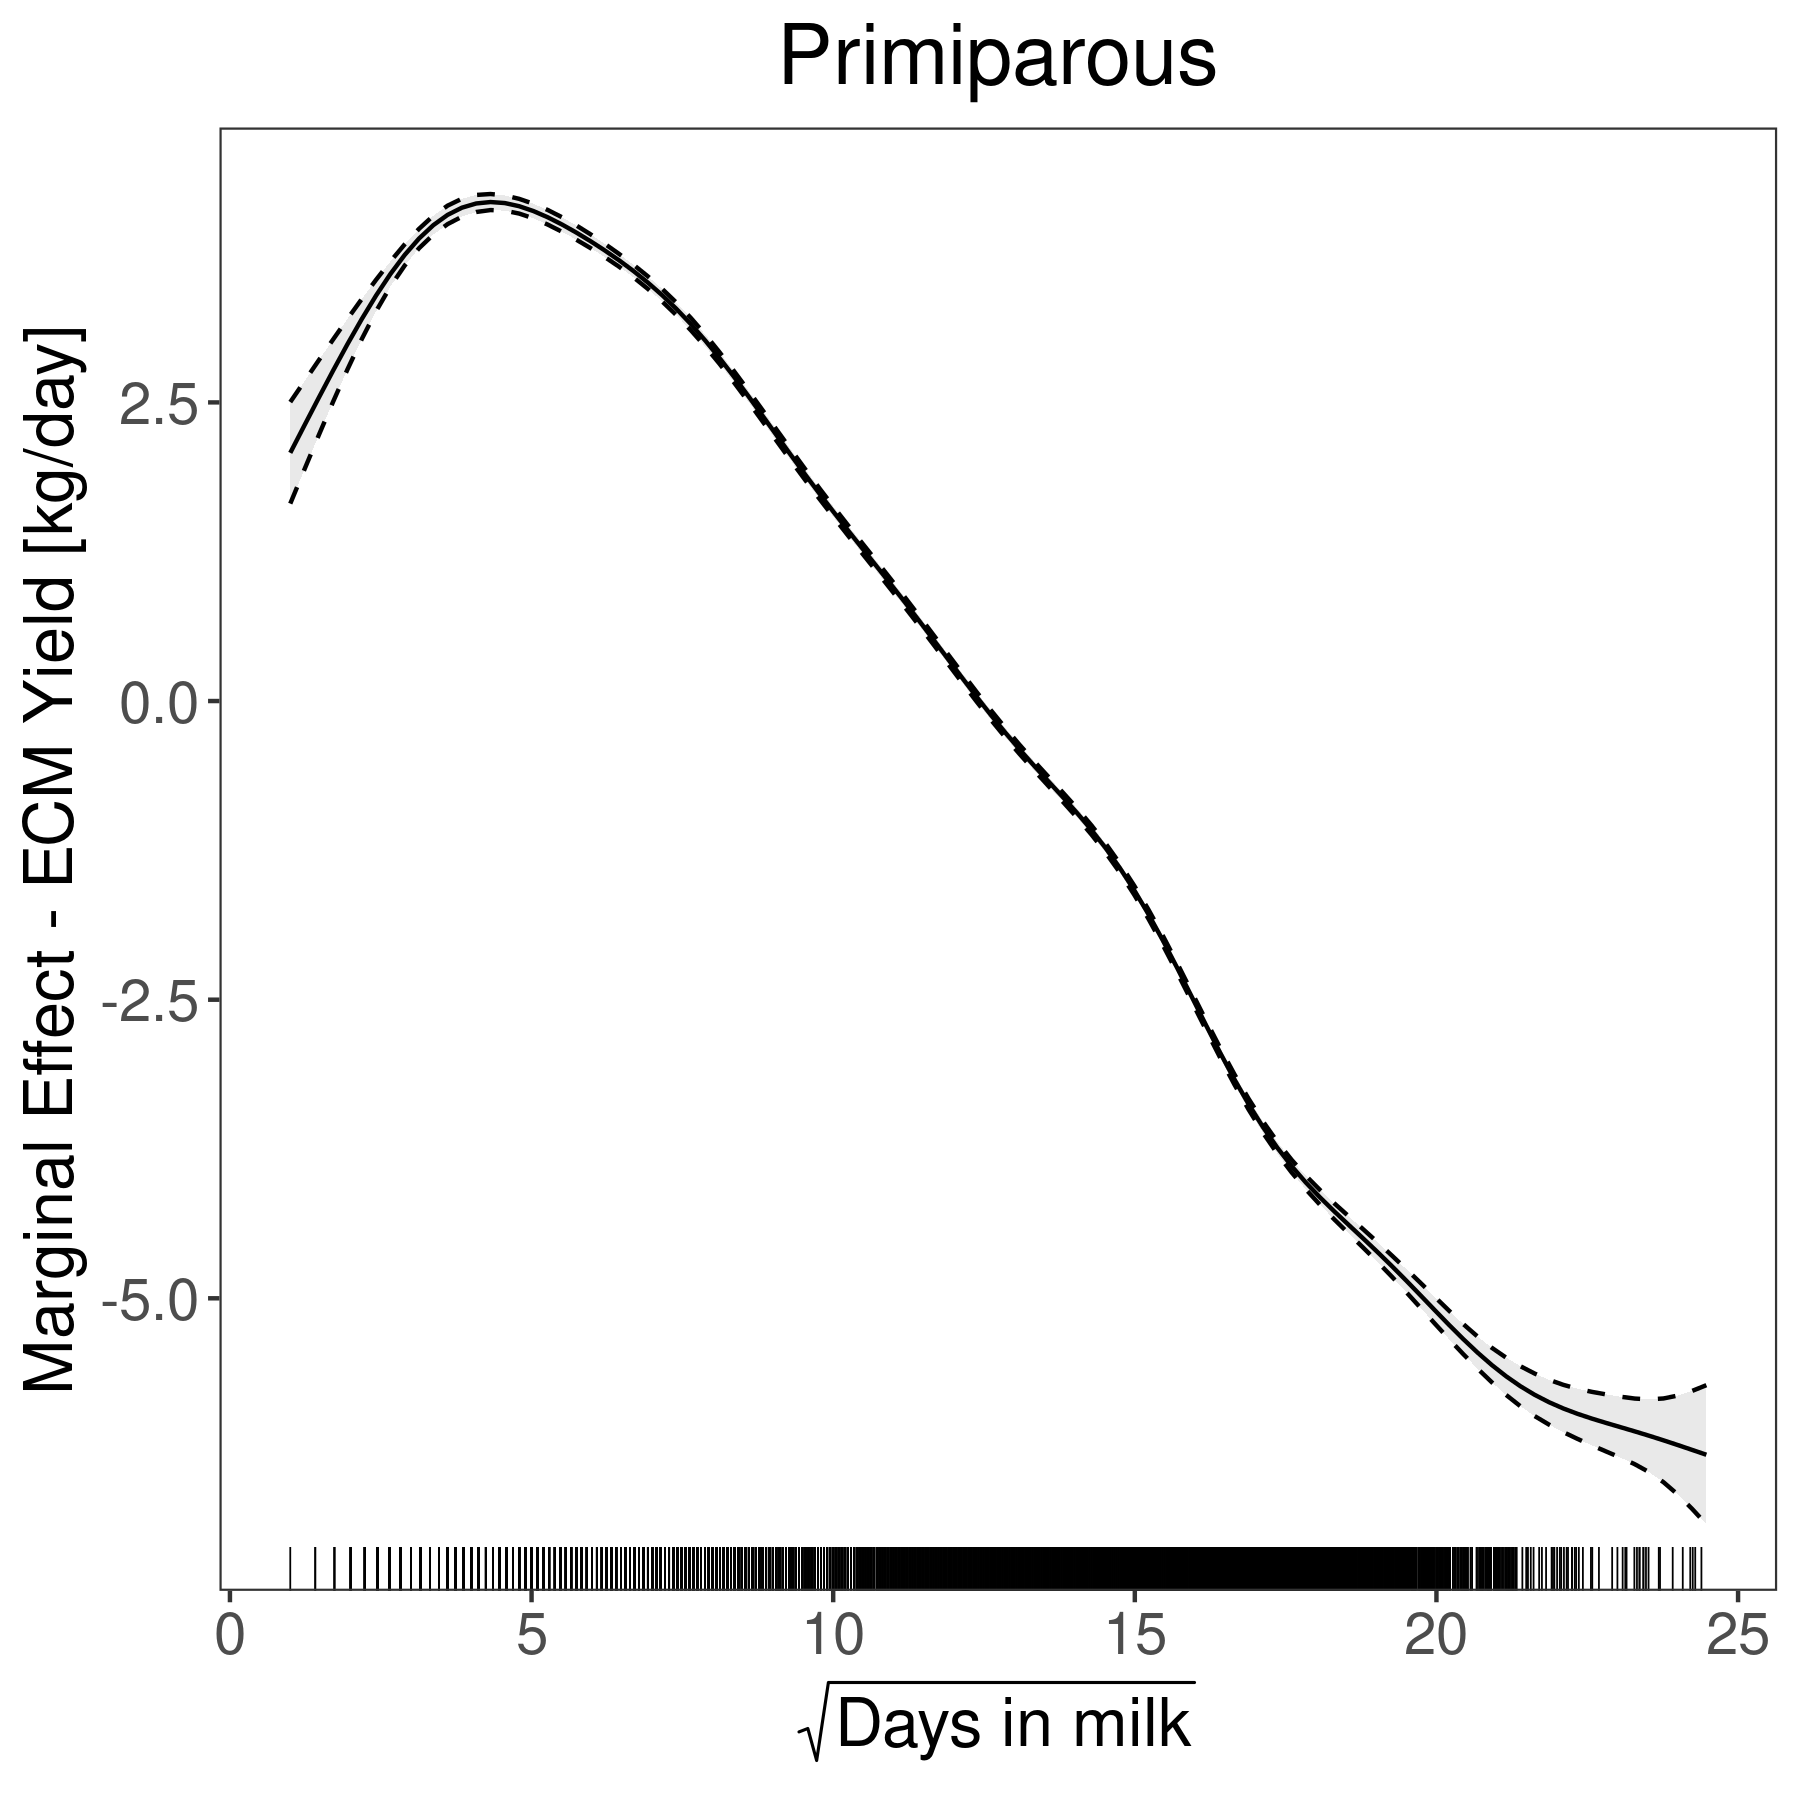
\includegraphics[width=\textwidth]{thesis/figures/models/ecm/after2010/sf_ecm_after2010/sf_ecm_after2010_marginal_dim_milk_primi.png}
    \end{subfigure}
    \begin{subfigure}[b]{0.45\textwidth}
        \centering
        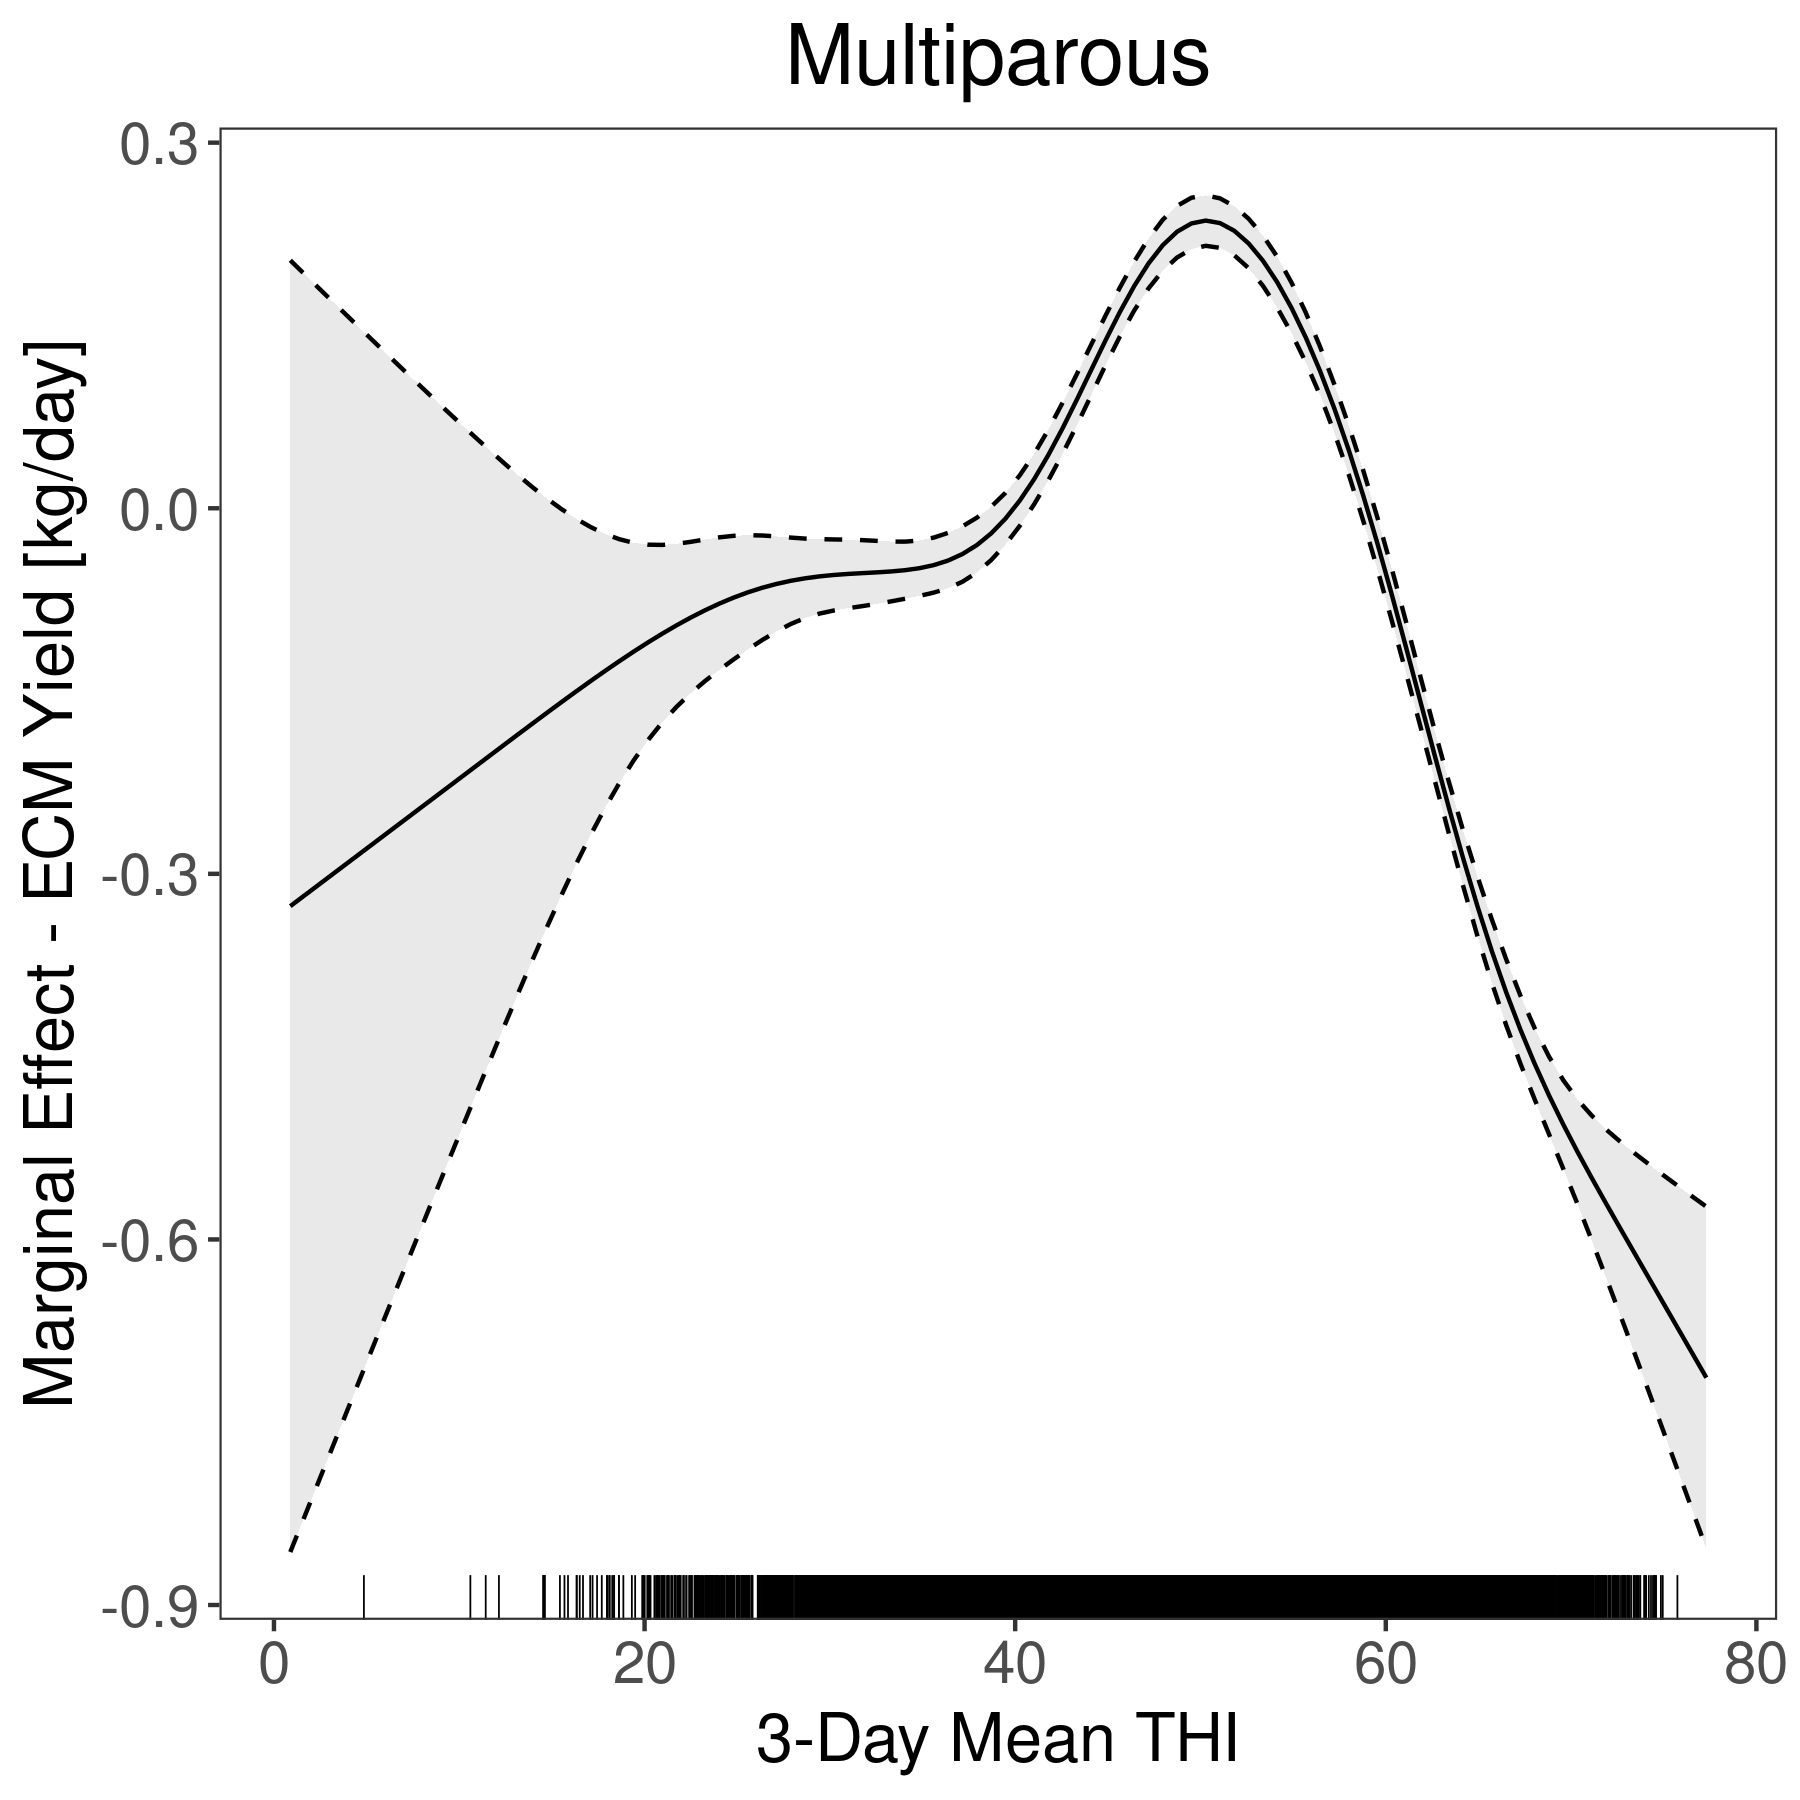
\includegraphics[width=\textwidth]{thesis/figures/models/ecm/after2010/sf_ecm_after2010/sf_ecm_after2010_marginal_thi_milk_multi.png}
    \end{subfigure}
    \hspace{0.05\textwidth} % Optional space between the figures
    \begin{subfigure}[b]{0.45\textwidth}
        \centering
        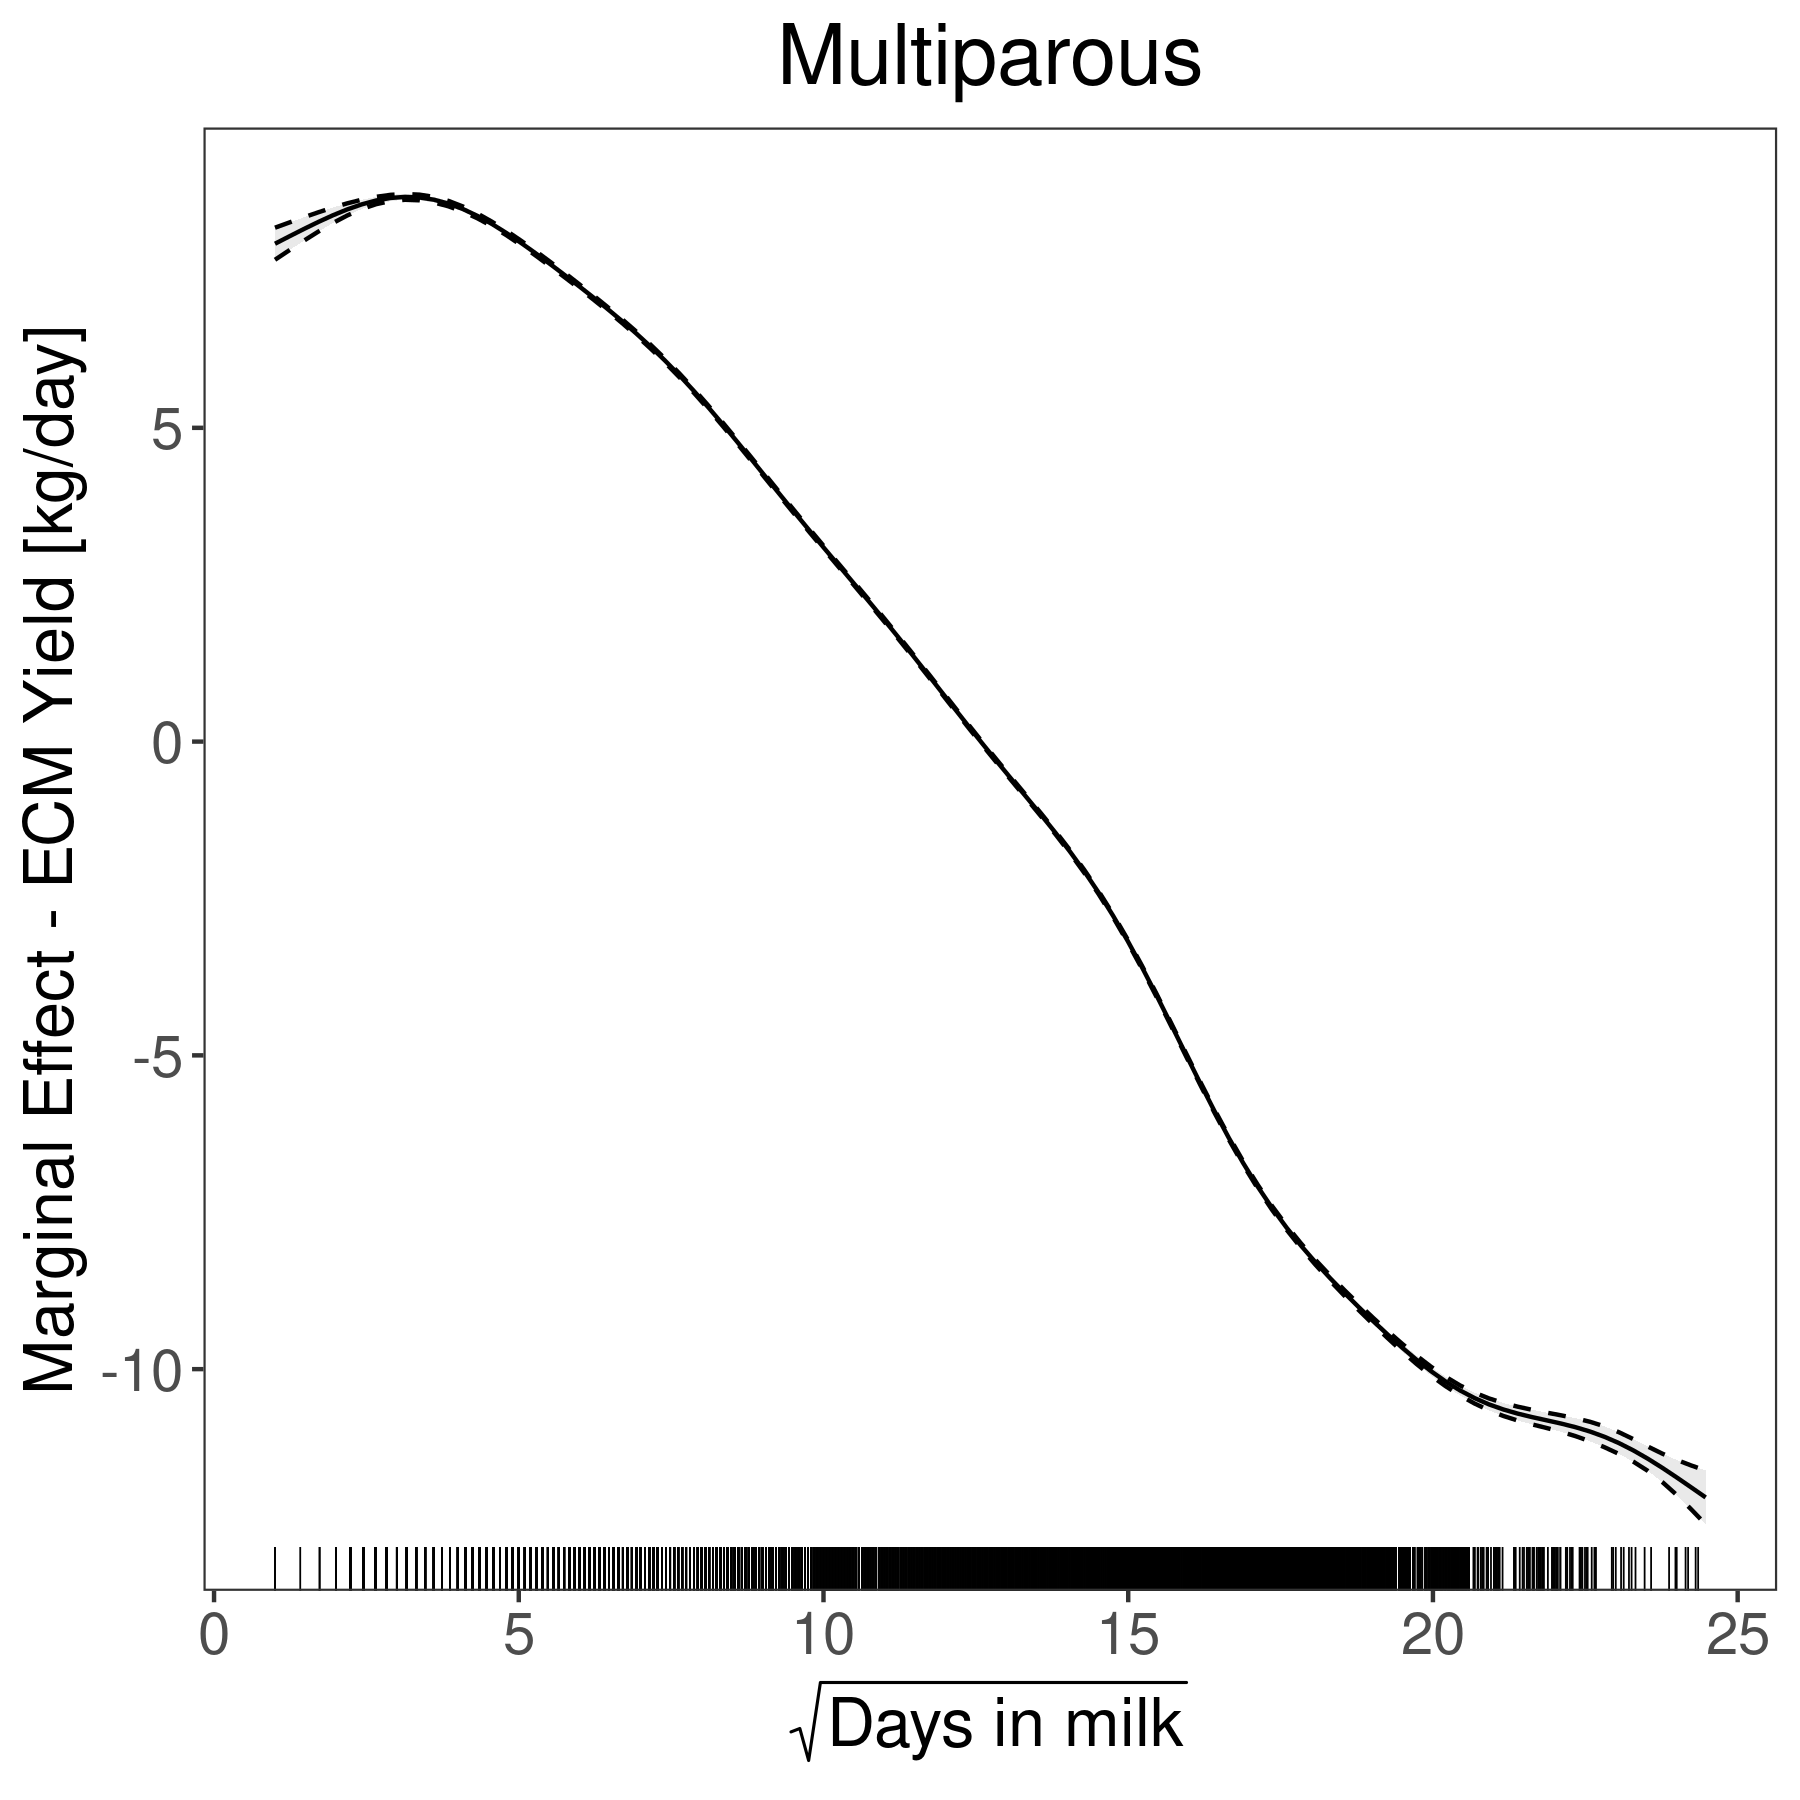
\includegraphics[width=\textwidth]{thesis/figures/models/ecm/after2010/sf_ecm_after2010/sf_ecm_after2010_marginal_dim_milk_multi.png}
    \end{subfigure}
    \caption[]{Swiss Fleckvieh: ECM Yield - 2011 - 2023 - THI Effect and Lactation Curve}
    \label{fig:main}
\end{figure}
\addtocontents{toc}{\protect\setcounter{tocdepth}{2}}